% Options for packages loaded elsewhere
\PassOptionsToPackage{unicode}{hyperref}
\PassOptionsToPackage{hyphens}{url}
%
\documentclass[
]{book}
\usepackage{amsmath,amssymb}
\usepackage{lmodern}
\usepackage{iftex}
\ifPDFTeX
  \usepackage[T1]{fontenc}
  \usepackage[utf8]{inputenc}
  \usepackage{textcomp} % provide euro and other symbols
\else % if luatex or xetex
  \usepackage{unicode-math}
  \defaultfontfeatures{Scale=MatchLowercase}
  \defaultfontfeatures[\rmfamily]{Ligatures=TeX,Scale=1}
\fi
% Use upquote if available, for straight quotes in verbatim environments
\IfFileExists{upquote.sty}{\usepackage{upquote}}{}
\IfFileExists{microtype.sty}{% use microtype if available
  \usepackage[]{microtype}
  \UseMicrotypeSet[protrusion]{basicmath} % disable protrusion for tt fonts
}{}
\makeatletter
\@ifundefined{KOMAClassName}{% if non-KOMA class
  \IfFileExists{parskip.sty}{%
    \usepackage{parskip}
  }{% else
    \setlength{\parindent}{0pt}
    \setlength{\parskip}{6pt plus 2pt minus 1pt}}
}{% if KOMA class
  \KOMAoptions{parskip=half}}
\makeatother
\usepackage{xcolor}
\usepackage{color}
\usepackage{fancyvrb}
\newcommand{\VerbBar}{|}
\newcommand{\VERB}{\Verb[commandchars=\\\{\}]}
\DefineVerbatimEnvironment{Highlighting}{Verbatim}{commandchars=\\\{\}}
% Add ',fontsize=\small' for more characters per line
\usepackage{framed}
\definecolor{shadecolor}{RGB}{248,248,248}
\newenvironment{Shaded}{\begin{snugshade}}{\end{snugshade}}
\newcommand{\AlertTok}[1]{\textcolor[rgb]{0.94,0.16,0.16}{#1}}
\newcommand{\AnnotationTok}[1]{\textcolor[rgb]{0.56,0.35,0.01}{\textbf{\textit{#1}}}}
\newcommand{\AttributeTok}[1]{\textcolor[rgb]{0.77,0.63,0.00}{#1}}
\newcommand{\BaseNTok}[1]{\textcolor[rgb]{0.00,0.00,0.81}{#1}}
\newcommand{\BuiltInTok}[1]{#1}
\newcommand{\CharTok}[1]{\textcolor[rgb]{0.31,0.60,0.02}{#1}}
\newcommand{\CommentTok}[1]{\textcolor[rgb]{0.56,0.35,0.01}{\textit{#1}}}
\newcommand{\CommentVarTok}[1]{\textcolor[rgb]{0.56,0.35,0.01}{\textbf{\textit{#1}}}}
\newcommand{\ConstantTok}[1]{\textcolor[rgb]{0.00,0.00,0.00}{#1}}
\newcommand{\ControlFlowTok}[1]{\textcolor[rgb]{0.13,0.29,0.53}{\textbf{#1}}}
\newcommand{\DataTypeTok}[1]{\textcolor[rgb]{0.13,0.29,0.53}{#1}}
\newcommand{\DecValTok}[1]{\textcolor[rgb]{0.00,0.00,0.81}{#1}}
\newcommand{\DocumentationTok}[1]{\textcolor[rgb]{0.56,0.35,0.01}{\textbf{\textit{#1}}}}
\newcommand{\ErrorTok}[1]{\textcolor[rgb]{0.64,0.00,0.00}{\textbf{#1}}}
\newcommand{\ExtensionTok}[1]{#1}
\newcommand{\FloatTok}[1]{\textcolor[rgb]{0.00,0.00,0.81}{#1}}
\newcommand{\FunctionTok}[1]{\textcolor[rgb]{0.00,0.00,0.00}{#1}}
\newcommand{\ImportTok}[1]{#1}
\newcommand{\InformationTok}[1]{\textcolor[rgb]{0.56,0.35,0.01}{\textbf{\textit{#1}}}}
\newcommand{\KeywordTok}[1]{\textcolor[rgb]{0.13,0.29,0.53}{\textbf{#1}}}
\newcommand{\NormalTok}[1]{#1}
\newcommand{\OperatorTok}[1]{\textcolor[rgb]{0.81,0.36,0.00}{\textbf{#1}}}
\newcommand{\OtherTok}[1]{\textcolor[rgb]{0.56,0.35,0.01}{#1}}
\newcommand{\PreprocessorTok}[1]{\textcolor[rgb]{0.56,0.35,0.01}{\textit{#1}}}
\newcommand{\RegionMarkerTok}[1]{#1}
\newcommand{\SpecialCharTok}[1]{\textcolor[rgb]{0.00,0.00,0.00}{#1}}
\newcommand{\SpecialStringTok}[1]{\textcolor[rgb]{0.31,0.60,0.02}{#1}}
\newcommand{\StringTok}[1]{\textcolor[rgb]{0.31,0.60,0.02}{#1}}
\newcommand{\VariableTok}[1]{\textcolor[rgb]{0.00,0.00,0.00}{#1}}
\newcommand{\VerbatimStringTok}[1]{\textcolor[rgb]{0.31,0.60,0.02}{#1}}
\newcommand{\WarningTok}[1]{\textcolor[rgb]{0.56,0.35,0.01}{\textbf{\textit{#1}}}}
\usepackage{longtable,booktabs,array}
\usepackage{calc} % for calculating minipage widths
% Correct order of tables after \paragraph or \subparagraph
\usepackage{etoolbox}
\makeatletter
\patchcmd\longtable{\par}{\if@noskipsec\mbox{}\fi\par}{}{}
\makeatother
% Allow footnotes in longtable head/foot
\IfFileExists{footnotehyper.sty}{\usepackage{footnotehyper}}{\usepackage{footnote}}
\makesavenoteenv{longtable}
\usepackage{graphicx}
\makeatletter
\def\maxwidth{\ifdim\Gin@nat@width>\linewidth\linewidth\else\Gin@nat@width\fi}
\def\maxheight{\ifdim\Gin@nat@height>\textheight\textheight\else\Gin@nat@height\fi}
\makeatother
% Scale images if necessary, so that they will not overflow the page
% margins by default, and it is still possible to overwrite the defaults
% using explicit options in \includegraphics[width, height, ...]{}
\setkeys{Gin}{width=\maxwidth,height=\maxheight,keepaspectratio}
% Set default figure placement to htbp
\makeatletter
\def\fps@figure{htbp}
\makeatother
\setlength{\emergencystretch}{3em} % prevent overfull lines
\providecommand{\tightlist}{%
  \setlength{\itemsep}{0pt}\setlength{\parskip}{0pt}}
\setcounter{secnumdepth}{5}
\ifLuaTeX
\usepackage[bidi=basic]{babel}
\else
\usepackage[bidi=default]{babel}
\fi
\babelprovide[main,import]{brazilian}
% get rid of language-specific shorthands (see #6817):
\let\LanguageShortHands\languageshorthands
\def\languageshorthands#1{}
\usepackage{booktabs}
\ifLuaTeX
  \usepackage{selnolig}  % disable illegal ligatures
\fi
\usepackage[]{natbib}
\bibliographystyle{plainnat}
\IfFileExists{bookmark.sty}{\usepackage{bookmark}}{\usepackage{hyperref}}
\IfFileExists{xurl.sty}{\usepackage{xurl}}{} % add URL line breaks if available
\urlstyle{same} % disable monospaced font for URLs
\hypersetup{
  pdftitle={Learning R packages},
  pdfauthor={Cristian Villegas},
  pdflang={Pt-Br},
  hidelinks,
  pdfcreator={LaTeX via pandoc}}

\title{Learning R packages}
\author{Cristian Villegas}
\date{2023-05-15}

\begin{document}
\maketitle

{
\setcounter{tocdepth}{1}
\tableofcontents
}
\hypertarget{intro}{%
\chapter{Intro}\label{intro}}

\hypertarget{carrega-pacotes-a-serem-usados}{%
\section{Carrega pacotes a serem usados}\label{carrega-pacotes-a-serem-usados}}

\begin{Shaded}
\begin{Highlighting}[]
\CommentTok{\#install.packages("tidyverse") }
\CommentTok{\#install.packages("dplyr")     }
\CommentTok{\#install.packages("tidyr")     }
\CommentTok{\#install.packages("ggplot2")   }

\FunctionTok{library}\NormalTok{(tidyverse)}
\CommentTok{\# Manipulação de dados}
\CommentTok{\#library(dplyr)}

\CommentTok{\# Visualização de gráficos}
\FunctionTok{library}\NormalTok{(ggplot2)}
\FunctionTok{library}\NormalTok{(gridExtra)}
\FunctionTok{library}\NormalTok{(patchwork)}
\FunctionTok{library}\NormalTok{(plotly)}
\FunctionTok{library}\NormalTok{(esquisse)}

\CommentTok{\# Para dados gráfico de perfis}
\FunctionTok{library}\NormalTok{(nlme)}
\end{Highlighting}
\end{Shaded}

\hypertarget{alguns-atalhos-no-rstudio}{%
\section{Alguns atalhos no Rstudio}\label{alguns-atalhos-no-rstudio}}

Para considerar

\begin{quote}
Operador Pipe (\%\textgreater\%): Ctrl + Shift + M (Windows) ou Cmd + Shift + M (Mac).
\end{quote}

\begin{quote}
Criar novos chunks: Ctrl + Alt + I (Windows) ou Cmd + Option + I (Mac).
\end{quote}

\hypertarget{dplyr-60-minutos}{%
\chapter{dplyr (60 minutos)}\label{dplyr-60-minutos}}

\hypertarget{carrega-pacotes-a-serem-usados-1}{%
\section{Carrega pacotes a serem usados}\label{carrega-pacotes-a-serem-usados-1}}

\begin{Shaded}
\begin{Highlighting}[]
\CommentTok{\#install.packages("tidyverse") }
\CommentTok{\#install.packages("dplyr")     }
\CommentTok{\#install.packages("tidyr")     }
\CommentTok{\#install.packages("ggplot2")   }

\FunctionTok{library}\NormalTok{(tidyverse)}
\CommentTok{\# Manipulação de dados}
\CommentTok{\#library(dplyr)}

\CommentTok{\# Visualização de gráficos}
\FunctionTok{library}\NormalTok{(ggplot2)}
\FunctionTok{library}\NormalTok{(gridExtra)}
\FunctionTok{library}\NormalTok{(patchwork)}
\FunctionTok{library}\NormalTok{(plotly)}
\FunctionTok{library}\NormalTok{(esquisse)}

\CommentTok{\# Para dados gráfico de perfis}
\FunctionTok{library}\NormalTok{(nlme)}
\end{Highlighting}
\end{Shaded}

\hypertarget{descriuxe7uxe3o-dos-dados-mpg}{%
\section{\texorpdfstring{Descrição dos dados \texttt{mpg}}{Descrição dos dados mpg}}\label{descriuxe7uxe3o-dos-dados-mpg}}

Dados de economia de combustível de 1999 a 2008 para \emph{38 modelos populares de carros}. Este conjunto de dados contém um subconjunto dos dados de economia de combustível que a EPA disponibiliza em \emph{\url{https://fueleconomy.gov/}}. Ele contém apenas modelos que tiveram um novo lançamento a cada ano entre 1999 e 2008 - isso foi usado como um substituto para a popularidade do carro. Um \emph{data frame} com 234 linhas e 11 variáveis:

\begin{itemize}
\item
  \emph{manufacturer} nome do fabricante
\item
  \emph{model} nome do modelo
\item
  \emph{displ} cilindrada do motor, em litros
\item
  \emph{year} ano de fabricação
\item
  \emph{cyl} número de cilindros
\item
  \emph{trans} tipo de transmissão
\item
  \emph{drv} o tipo de trem de força, onde \textbf{f = tração dianteira}, \textbf{r = tração traseira} e \textbf{4 = 4wd}
\item
  \emph{cty} milhas urbanas por galão
\item
  \emph{hwy} milhas rodoviárias por galão
\item
  \emph{fl} tipo de combustível
\item
  \emph{class} ``tipo'' de carro
\end{itemize}

\begin{Shaded}
\begin{Highlighting}[]
\CommentTok{\#help("mpg")}
\FunctionTok{library}\NormalTok{(tidyverse)}
\NormalTok{dados }\OtherTok{\textless{}{-}}\NormalTok{ mpg}
\FunctionTok{glimpse}\NormalTok{(dados)}
\end{Highlighting}
\end{Shaded}

\begin{verbatim}
## Rows: 234
## Columns: 11
## $ manufacturer <chr> "audi", "audi", "audi", "audi", "audi", "audi", "audi", "~
## $ model        <chr> "a4", "a4", "a4", "a4", "a4", "a4", "a4", "a4 quattro", "~
## $ displ        <dbl> 1.8, 1.8, 2.0, 2.0, 2.8, 2.8, 3.1, 1.8, 1.8, 2.0, 2.0, 2.~
## $ year         <int> 1999, 1999, 2008, 2008, 1999, 1999, 2008, 1999, 1999, 200~
## $ cyl          <int> 4, 4, 4, 4, 6, 6, 6, 4, 4, 4, 4, 6, 6, 6, 6, 6, 6, 8, 8, ~
## $ trans        <chr> "auto(l5)", "manual(m5)", "manual(m6)", "auto(av)", "auto~
## $ drv          <chr> "f", "f", "f", "f", "f", "f", "f", "4", "4", "4", "4", "4~
## $ cty          <int> 18, 21, 20, 21, 16, 18, 18, 18, 16, 20, 19, 15, 17, 17, 1~
## $ hwy          <int> 29, 29, 31, 30, 26, 26, 27, 26, 25, 28, 27, 25, 25, 25, 2~
## $ fl           <chr> "p", "p", "p", "p", "p", "p", "p", "p", "p", "p", "p", "p~
## $ class        <chr> "compact", "compact", "compact", "compact", "compact", "c~
\end{verbatim}

\begin{Shaded}
\begin{Highlighting}[]
\NormalTok{dados }\OtherTok{\textless{}{-}} \FunctionTok{mutate}\NormalTok{(}\AttributeTok{.data =}\NormalTok{ dados, }
                \FunctionTok{across}\NormalTok{(}\FunctionTok{where}\NormalTok{(is.character), }
\NormalTok{                as.factor))}
\CommentTok{\#View(df) }
\FunctionTok{glimpse}\NormalTok{(dados)}
\end{Highlighting}
\end{Shaded}

\begin{verbatim}
## Rows: 234
## Columns: 11
## $ manufacturer <fct> audi, audi, audi, audi, audi, audi, audi, audi, audi, aud~
## $ model        <fct> a4, a4, a4, a4, a4, a4, a4, a4 quattro, a4 quattro, a4 qu~
## $ displ        <dbl> 1.8, 1.8, 2.0, 2.0, 2.8, 2.8, 3.1, 1.8, 1.8, 2.0, 2.0, 2.~
## $ year         <int> 1999, 1999, 2008, 2008, 1999, 1999, 2008, 1999, 1999, 200~
## $ cyl          <int> 4, 4, 4, 4, 6, 6, 6, 4, 4, 4, 4, 6, 6, 6, 6, 6, 6, 8, 8, ~
## $ trans        <fct> auto(l5), manual(m5), manual(m6), auto(av), auto(l5), man~
## $ drv          <fct> f, f, f, f, f, f, f, 4, 4, 4, 4, 4, 4, 4, 4, 4, 4, 4, r, ~
## $ cty          <int> 18, 21, 20, 21, 16, 18, 18, 18, 16, 20, 19, 15, 17, 17, 1~
## $ hwy          <int> 29, 29, 31, 30, 26, 26, 27, 26, 25, 28, 27, 25, 25, 25, 2~
## $ fl           <fct> p, p, p, p, p, p, p, p, p, p, p, p, p, p, p, p, p, p, r, ~
## $ class        <fct> compact, compact, compact, compact, compact, compact, com~
\end{verbatim}

\hypertarget{lista-de-funuxe7uxf5es-do-pacote-dplyr}{%
\section{Lista de funções do pacote dplyr}\label{lista-de-funuxe7uxf5es-do-pacote-dplyr}}

\begin{Shaded}
\begin{Highlighting}[]
\FunctionTok{ls}\NormalTok{(}\StringTok{"package:dplyr"}\NormalTok{)}
\end{Highlighting}
\end{Shaded}

\begin{verbatim}
##   [1] "%>%"                   "across"                "add_count"            
##   [4] "add_count_"            "add_row"               "add_rownames"         
##   [7] "add_tally"             "add_tally_"            "all_equal"            
##  [10] "all_of"                "all_vars"              "anti_join"            
##  [13] "any_of"                "any_vars"              "arrange"              
##  [16] "arrange_"              "arrange_all"           "arrange_at"           
##  [19] "arrange_if"            "as.tbl"                "as_data_frame"        
##  [22] "as_label"              "as_tibble"             "auto_copy"            
##  [25] "band_instruments"      "band_instruments2"     "band_members"         
##  [28] "bench_tbls"            "between"               "bind_cols"            
##  [31] "bind_rows"             "c_across"              "case_match"           
##  [34] "case_when"             "changes"               "check_dbplyr"         
##  [37] "coalesce"              "collapse"              "collect"              
##  [40] "combine"               "common_by"             "compare_tbls"         
##  [43] "compare_tbls2"         "compute"               "consecutive_id"       
##  [46] "contains"              "copy_to"               "count"                
##  [49] "count_"                "cross_join"            "cumall"               
##  [52] "cumany"                "cume_dist"             "cummean"              
##  [55] "cur_column"            "cur_data"              "cur_data_all"         
##  [58] "cur_group"             "cur_group_id"          "cur_group_rows"       
##  [61] "current_vars"          "data_frame"            "db_analyze"           
##  [64] "db_begin"              "db_commit"             "db_create_index"      
##  [67] "db_create_indexes"     "db_create_table"       "db_data_type"         
##  [70] "db_desc"               "db_drop_table"         "db_explain"           
##  [73] "db_has_table"          "db_insert_into"        "db_list_tables"       
##  [76] "db_query_fields"       "db_query_rows"         "db_rollback"          
##  [79] "db_save_query"         "db_write_table"        "dense_rank"           
##  [82] "desc"                  "dim_desc"              "distinct"             
##  [85] "distinct_"             "distinct_all"          "distinct_at"          
##  [88] "distinct_if"           "distinct_prepare"      "do"                   
##  [91] "do_"                   "dplyr_col_modify"      "dplyr_reconstruct"    
##  [94] "dplyr_row_slice"       "ends_with"             "enexpr"               
##  [97] "enexprs"               "enquo"                 "enquos"               
## [100] "ensym"                 "ensyms"                "eval_tbls"            
## [103] "eval_tbls2"            "everything"            "explain"              
## [106] "expr"                  "failwith"              "filter"               
## [109] "filter_"               "filter_all"            "filter_at"            
## [112] "filter_if"             "first"                 "full_join"            
## [115] "funs"                  "funs_"                 "glimpse"              
## [118] "group_by"              "group_by_"             "group_by_all"         
## [121] "group_by_at"           "group_by_drop_default" "group_by_if"          
## [124] "group_by_prepare"      "group_cols"            "group_data"           
## [127] "group_indices"         "group_indices_"        "group_keys"           
## [130] "group_map"             "group_modify"          "group_nest"           
## [133] "group_rows"            "group_size"            "group_split"          
## [136] "group_trim"            "group_vars"            "group_walk"           
## [139] "grouped_df"            "groups"                "id"                   
## [142] "ident"                 "if_all"                "if_any"               
## [145] "if_else"               "inner_join"            "intersect"            
## [148] "is.grouped_df"         "is.src"                "is.tbl"               
## [151] "is_grouped_df"         "join_by"               "lag"                  
## [154] "last"                  "last_col"              "last_dplyr_warnings"  
## [157] "lead"                  "left_join"             "location"             
## [160] "lst"                   "make_tbl"              "matches"              
## [163] "min_rank"              "mutate"                "mutate_"              
## [166] "mutate_all"            "mutate_at"             "mutate_each"          
## [169] "mutate_each_"          "mutate_if"             "n"                    
## [172] "n_distinct"            "n_groups"              "na_if"                
## [175] "near"                  "nest_by"               "nest_join"            
## [178] "new_grouped_df"        "new_rowwise_df"        "nth"                  
## [181] "ntile"                 "num_range"             "one_of"               
## [184] "order_by"              "percent_rank"          "pick"                 
## [187] "progress_estimated"    "pull"                  "quo"                  
## [190] "quo_name"              "quos"                  "recode"               
## [193] "recode_factor"         "reframe"               "relocate"             
## [196] "rename"                "rename_"               "rename_all"           
## [199] "rename_at"             "rename_if"             "rename_vars"          
## [202] "rename_vars_"          "rename_with"           "right_join"           
## [205] "row_number"            "rows_append"           "rows_delete"          
## [208] "rows_insert"           "rows_patch"            "rows_update"          
## [211] "rows_upsert"           "rowwise"               "same_src"             
## [214] "sample_frac"           "sample_n"              "select"               
## [217] "select_"               "select_all"            "select_at"            
## [220] "select_if"             "select_var"            "select_vars"          
## [223] "select_vars_"          "semi_join"             "setdiff"              
## [226] "setequal"              "show_query"            "slice"                
## [229] "slice_"                "slice_head"            "slice_max"            
## [232] "slice_min"             "slice_sample"          "slice_tail"           
## [235] "sql"                   "sql_escape_ident"      "sql_escape_string"    
## [238] "sql_join"              "sql_select"            "sql_semi_join"        
## [241] "sql_set_op"            "sql_subquery"          "sql_translate_env"    
## [244] "src"                   "src_df"                "src_local"            
## [247] "src_mysql"             "src_postgres"          "src_sqlite"           
## [250] "src_tbls"              "starts_with"           "starwars"             
## [253] "storms"                "summarise"             "summarise_"           
## [256] "summarise_all"         "summarise_at"          "summarise_each"       
## [259] "summarise_each_"       "summarise_if"          "summarize"            
## [262] "summarize_"            "summarize_all"         "summarize_at"         
## [265] "summarize_each"        "summarize_each_"       "summarize_if"         
## [268] "sym"                   "symdiff"               "syms"                 
## [271] "tally"                 "tally_"                "tbl"                  
## [274] "tbl_df"                "tbl_nongroup_vars"     "tbl_ptype"            
## [277] "tbl_vars"              "tibble"                "top_frac"             
## [280] "top_n"                 "transmute"             "transmute_"           
## [283] "transmute_all"         "transmute_at"          "transmute_if"         
## [286] "tribble"               "type_sum"              "ungroup"              
## [289] "union"                 "union_all"             "validate_grouped_df"  
## [292] "validate_rowwise_df"   "vars"                  "where"                
## [295] "with_groups"           "with_order"            "wrap_dbplyr_obj"
\end{verbatim}

\hypertarget{operador-pipe}{%
\section{Operador Pipe}\label{operador-pipe}}

\begin{Shaded}
\begin{Highlighting}[]
\FunctionTok{sqrt}\NormalTok{(}\FunctionTok{log}\NormalTok{(}\DecValTok{44}\NormalTok{))}
\end{Highlighting}
\end{Shaded}

\begin{verbatim}
## [1] 1.945299
\end{verbatim}

\begin{Shaded}
\begin{Highlighting}[]
\DecValTok{44} \SpecialCharTok{\%\textgreater{}\%}\NormalTok{ log }\SpecialCharTok{\%\textgreater{}\%}\NormalTok{ sqrt}
\end{Highlighting}
\end{Shaded}

\begin{verbatim}
## [1] 1.945299
\end{verbatim}

\hypertarget{select-para-colunas}{%
\section{select() para colunas}\label{select-para-colunas}}

\begin{Shaded}
\begin{Highlighting}[]
\FunctionTok{select}\NormalTok{(dados, manufacturer, model, year)}
\end{Highlighting}
\end{Shaded}

\begin{verbatim}
## # A tibble: 234 x 3
##    manufacturer model       year
##    <fct>        <fct>      <int>
##  1 audi         a4          1999
##  2 audi         a4          1999
##  3 audi         a4          2008
##  4 audi         a4          2008
##  5 audi         a4          1999
##  6 audi         a4          1999
##  7 audi         a4          2008
##  8 audi         a4 quattro  1999
##  9 audi         a4 quattro  1999
## 10 audi         a4 quattro  2008
## # ... with 224 more rows
\end{verbatim}

\begin{Shaded}
\begin{Highlighting}[]
\FunctionTok{select}\NormalTok{(dados, }\FunctionTok{starts\_with}\NormalTok{(}\StringTok{"m"}\NormalTok{))}
\end{Highlighting}
\end{Shaded}

\begin{verbatim}
## # A tibble: 234 x 2
##    manufacturer model     
##    <fct>        <fct>     
##  1 audi         a4        
##  2 audi         a4        
##  3 audi         a4        
##  4 audi         a4        
##  5 audi         a4        
##  6 audi         a4        
##  7 audi         a4        
##  8 audi         a4 quattro
##  9 audi         a4 quattro
## 10 audi         a4 quattro
## # ... with 224 more rows
\end{verbatim}

\begin{Shaded}
\begin{Highlighting}[]
\FunctionTok{select}\NormalTok{(dados, }\FunctionTok{contains}\NormalTok{(}\StringTok{"r"}\NormalTok{))}
\end{Highlighting}
\end{Shaded}

\begin{verbatim}
## # A tibble: 234 x 4
##    manufacturer  year trans      drv  
##    <fct>        <int> <fct>      <fct>
##  1 audi          1999 auto(l5)   f    
##  2 audi          1999 manual(m5) f    
##  3 audi          2008 manual(m6) f    
##  4 audi          2008 auto(av)   f    
##  5 audi          1999 auto(l5)   f    
##  6 audi          1999 manual(m5) f    
##  7 audi          2008 auto(av)   f    
##  8 audi          1999 manual(m5) 4    
##  9 audi          1999 auto(l5)   4    
## 10 audi          2008 manual(m6) 4    
## # ... with 224 more rows
\end{verbatim}

\begin{Shaded}
\begin{Highlighting}[]
\FunctionTok{select}\NormalTok{(dados, }\FunctionTok{ends\_with}\NormalTok{(}\StringTok{"y"}\NormalTok{))}
\end{Highlighting}
\end{Shaded}

\begin{verbatim}
## # A tibble: 234 x 2
##      cty   hwy
##    <int> <int>
##  1    18    29
##  2    21    29
##  3    20    31
##  4    21    30
##  5    16    26
##  6    18    26
##  7    18    27
##  8    18    26
##  9    16    25
## 10    20    28
## # ... with 224 more rows
\end{verbatim}

\begin{Shaded}
\begin{Highlighting}[]
\FunctionTok{select}\NormalTok{(dados, }\FunctionTok{matches}\NormalTok{(}\StringTok{"[abc]"}\NormalTok{))}
\end{Highlighting}
\end{Shaded}

\begin{verbatim}
## # A tibble: 234 x 6
##    manufacturer  year   cyl trans        cty class  
##    <fct>        <int> <int> <fct>      <int> <fct>  
##  1 audi          1999     4 auto(l5)      18 compact
##  2 audi          1999     4 manual(m5)    21 compact
##  3 audi          2008     4 manual(m6)    20 compact
##  4 audi          2008     4 auto(av)      21 compact
##  5 audi          1999     6 auto(l5)      16 compact
##  6 audi          1999     6 manual(m5)    18 compact
##  7 audi          2008     6 auto(av)      18 compact
##  8 audi          1999     4 manual(m5)    18 compact
##  9 audi          1999     4 auto(l5)      16 compact
## 10 audi          2008     4 manual(m6)    20 compact
## # ... with 224 more rows
\end{verbatim}

\begin{Shaded}
\begin{Highlighting}[]
\FunctionTok{select}\NormalTok{(dados, }\FunctionTok{starts\_with}\NormalTok{(}\StringTok{"m"}\NormalTok{), }\FunctionTok{starts\_with}\NormalTok{(}\StringTok{"c"}\NormalTok{)) }
\end{Highlighting}
\end{Shaded}

\begin{verbatim}
## # A tibble: 234 x 5
##    manufacturer model        cyl   cty class  
##    <fct>        <fct>      <int> <int> <fct>  
##  1 audi         a4             4    18 compact
##  2 audi         a4             4    21 compact
##  3 audi         a4             4    20 compact
##  4 audi         a4             4    21 compact
##  5 audi         a4             6    16 compact
##  6 audi         a4             6    18 compact
##  7 audi         a4             6    18 compact
##  8 audi         a4 quattro     4    18 compact
##  9 audi         a4 quattro     4    16 compact
## 10 audi         a4 quattro     4    20 compact
## # ... with 224 more rows
\end{verbatim}

\begin{Shaded}
\begin{Highlighting}[]
\FunctionTok{select}\NormalTok{(dados, }\FunctionTok{ends\_with}\NormalTok{(}\StringTok{"l"}\NormalTok{), }\FunctionTok{ends\_with}\NormalTok{(}\StringTok{"s"}\NormalTok{)) }
\end{Highlighting}
\end{Shaded}

\begin{verbatim}
## # A tibble: 234 x 6
##    model      displ   cyl fl    trans      class  
##    <fct>      <dbl> <int> <fct> <fct>      <fct>  
##  1 a4           1.8     4 p     auto(l5)   compact
##  2 a4           1.8     4 p     manual(m5) compact
##  3 a4           2       4 p     manual(m6) compact
##  4 a4           2       4 p     auto(av)   compact
##  5 a4           2.8     6 p     auto(l5)   compact
##  6 a4           2.8     6 p     manual(m5) compact
##  7 a4           3.1     6 p     auto(av)   compact
##  8 a4 quattro   1.8     4 p     manual(m5) compact
##  9 a4 quattro   1.8     4 p     auto(l5)   compact
## 10 a4 quattro   2       4 p     manual(m6) compact
## # ... with 224 more rows
\end{verbatim}

\begin{Shaded}
\begin{Highlighting}[]
\FunctionTok{select}\NormalTok{(dados, }\DecValTok{1}\SpecialCharTok{:}\DecValTok{3}\NormalTok{)      }
\end{Highlighting}
\end{Shaded}

\begin{verbatim}
## # A tibble: 234 x 3
##    manufacturer model      displ
##    <fct>        <fct>      <dbl>
##  1 audi         a4           1.8
##  2 audi         a4           1.8
##  3 audi         a4           2  
##  4 audi         a4           2  
##  5 audi         a4           2.8
##  6 audi         a4           2.8
##  7 audi         a4           3.1
##  8 audi         a4 quattro   1.8
##  9 audi         a4 quattro   1.8
## 10 audi         a4 quattro   2  
## # ... with 224 more rows
\end{verbatim}

\begin{Shaded}
\begin{Highlighting}[]
\FunctionTok{select}\NormalTok{(dados, }\FunctionTok{c}\NormalTok{(}\DecValTok{2}\NormalTok{,}\DecValTok{5}\NormalTok{,}\DecValTok{7}\NormalTok{)) }
\end{Highlighting}
\end{Shaded}

\begin{verbatim}
## # A tibble: 234 x 3
##    model        cyl drv  
##    <fct>      <int> <fct>
##  1 a4             4 f    
##  2 a4             4 f    
##  3 a4             4 f    
##  4 a4             4 f    
##  5 a4             6 f    
##  6 a4             6 f    
##  7 a4             6 f    
##  8 a4 quattro     4 4    
##  9 a4 quattro     4 4    
## 10 a4 quattro     4 4    
## # ... with 224 more rows
\end{verbatim}

\begin{Shaded}
\begin{Highlighting}[]
\FunctionTok{select}\NormalTok{(dados, manufacturer}\SpecialCharTok{:}\NormalTok{cyl) }
\end{Highlighting}
\end{Shaded}

\begin{verbatim}
## # A tibble: 234 x 5
##    manufacturer model      displ  year   cyl
##    <fct>        <fct>      <dbl> <int> <int>
##  1 audi         a4           1.8  1999     4
##  2 audi         a4           1.8  1999     4
##  3 audi         a4           2    2008     4
##  4 audi         a4           2    2008     4
##  5 audi         a4           2.8  1999     6
##  6 audi         a4           2.8  1999     6
##  7 audi         a4           3.1  2008     6
##  8 audi         a4 quattro   1.8  1999     4
##  9 audi         a4 quattro   1.8  1999     4
## 10 audi         a4 quattro   2    2008     4
## # ... with 224 more rows
\end{verbatim}

\begin{Shaded}
\begin{Highlighting}[]
\FunctionTok{select}\NormalTok{(dados,}\SpecialCharTok{{-}}\NormalTok{(manufacturer}\SpecialCharTok{:}\NormalTok{cyl))}
\end{Highlighting}
\end{Shaded}

\begin{verbatim}
## # A tibble: 234 x 6
##    trans      drv     cty   hwy fl    class  
##    <fct>      <fct> <int> <int> <fct> <fct>  
##  1 auto(l5)   f        18    29 p     compact
##  2 manual(m5) f        21    29 p     compact
##  3 manual(m6) f        20    31 p     compact
##  4 auto(av)   f        21    30 p     compact
##  5 auto(l5)   f        16    26 p     compact
##  6 manual(m5) f        18    26 p     compact
##  7 auto(av)   f        18    27 p     compact
##  8 manual(m5) 4        18    26 p     compact
##  9 auto(l5)   4        16    25 p     compact
## 10 manual(m6) 4        20    28 p     compact
## # ... with 224 more rows
\end{verbatim}

\hypertarget{rename}{%
\section{rename()}\label{rename}}

\begin{Shaded}
\begin{Highlighting}[]
\NormalTok{dados1 }\OtherTok{\textless{}{-}} \FunctionTok{rename}\NormalTok{(dados, }
              \AttributeTok{mnfc =}\NormalTok{ manufacturer,}
              \AttributeTok{mod =}\NormalTok{ model)}
\NormalTok{dados1}
\end{Highlighting}
\end{Shaded}

\begin{verbatim}
## # A tibble: 234 x 11
##    mnfc  mod        displ  year   cyl trans      drv     cty   hwy fl    class  
##    <fct> <fct>      <dbl> <int> <int> <fct>      <fct> <int> <int> <fct> <fct>  
##  1 audi  a4           1.8  1999     4 auto(l5)   f        18    29 p     compact
##  2 audi  a4           1.8  1999     4 manual(m5) f        21    29 p     compact
##  3 audi  a4           2    2008     4 manual(m6) f        20    31 p     compact
##  4 audi  a4           2    2008     4 auto(av)   f        21    30 p     compact
##  5 audi  a4           2.8  1999     6 auto(l5)   f        16    26 p     compact
##  6 audi  a4           2.8  1999     6 manual(m5) f        18    26 p     compact
##  7 audi  a4           3.1  2008     6 auto(av)   f        18    27 p     compact
##  8 audi  a4 quattro   1.8  1999     4 manual(m5) 4        18    26 p     compact
##  9 audi  a4 quattro   1.8  1999     4 auto(l5)   4        16    25 p     compact
## 10 audi  a4 quattro   2    2008     4 manual(m6) 4        20    28 p     compact
## # ... with 224 more rows
\end{verbatim}

\begin{Shaded}
\begin{Highlighting}[]
\FunctionTok{select}\NormalTok{(dados,}
       \AttributeTok{mnfc =}\NormalTok{ manufacturer,}
       \AttributeTok{mod =}\NormalTok{ model)}
\end{Highlighting}
\end{Shaded}

\begin{verbatim}
## # A tibble: 234 x 2
##    mnfc  mod       
##    <fct> <fct>     
##  1 audi  a4        
##  2 audi  a4        
##  3 audi  a4        
##  4 audi  a4        
##  5 audi  a4        
##  6 audi  a4        
##  7 audi  a4        
##  8 audi  a4 quattro
##  9 audi  a4 quattro
## 10 audi  a4 quattro
## # ... with 224 more rows
\end{verbatim}

\begin{Shaded}
\begin{Highlighting}[]
\FunctionTok{select}\NormalTok{(dados,}
       \AttributeTok{mnfc =}\NormalTok{ manufacturer,}
       \AttributeTok{mod =}\NormalTok{ model,}
       \FunctionTok{everything}\NormalTok{())}
\end{Highlighting}
\end{Shaded}

\begin{verbatim}
## # A tibble: 234 x 11
##    mnfc  mod        displ  year   cyl trans      drv     cty   hwy fl    class  
##    <fct> <fct>      <dbl> <int> <int> <fct>      <fct> <int> <int> <fct> <fct>  
##  1 audi  a4           1.8  1999     4 auto(l5)   f        18    29 p     compact
##  2 audi  a4           1.8  1999     4 manual(m5) f        21    29 p     compact
##  3 audi  a4           2    2008     4 manual(m6) f        20    31 p     compact
##  4 audi  a4           2    2008     4 auto(av)   f        21    30 p     compact
##  5 audi  a4           2.8  1999     6 auto(l5)   f        16    26 p     compact
##  6 audi  a4           2.8  1999     6 manual(m5) f        18    26 p     compact
##  7 audi  a4           3.1  2008     6 auto(av)   f        18    27 p     compact
##  8 audi  a4 quattro   1.8  1999     4 manual(m5) 4        18    26 p     compact
##  9 audi  a4 quattro   1.8  1999     4 auto(l5)   4        16    25 p     compact
## 10 audi  a4 quattro   2    2008     4 manual(m6) 4        20    28 p     compact
## # ... with 224 more rows
\end{verbatim}

\hypertarget{mutate-para-colunas}{%
\section{mutate() para colunas}\label{mutate-para-colunas}}

\begin{Shaded}
\begin{Highlighting}[]
\FunctionTok{mutate}\NormalTok{(dados, }\AttributeTok{sqrt\_cty =} \FunctionTok{sqrt}\NormalTok{(cty))}
\end{Highlighting}
\end{Shaded}

\begin{verbatim}
## # A tibble: 234 x 12
##    manufac~1 model displ  year   cyl trans drv     cty   hwy fl    class sqrt_~2
##    <fct>     <fct> <dbl> <int> <int> <fct> <fct> <int> <int> <fct> <fct>   <dbl>
##  1 audi      a4      1.8  1999     4 auto~ f        18    29 p     comp~    4.24
##  2 audi      a4      1.8  1999     4 manu~ f        21    29 p     comp~    4.58
##  3 audi      a4      2    2008     4 manu~ f        20    31 p     comp~    4.47
##  4 audi      a4      2    2008     4 auto~ f        21    30 p     comp~    4.58
##  5 audi      a4      2.8  1999     6 auto~ f        16    26 p     comp~    4   
##  6 audi      a4      2.8  1999     6 manu~ f        18    26 p     comp~    4.24
##  7 audi      a4      3.1  2008     6 auto~ f        18    27 p     comp~    4.24
##  8 audi      a4 q~   1.8  1999     4 manu~ 4        18    26 p     comp~    4.24
##  9 audi      a4 q~   1.8  1999     4 auto~ 4        16    25 p     comp~    4   
## 10 audi      a4 q~   2    2008     4 manu~ 4        20    28 p     comp~    4.47
## # ... with 224 more rows, and abbreviated variable names 1: manufacturer,
## #   2: sqrt_cty
\end{verbatim}

\begin{Shaded}
\begin{Highlighting}[]
\FunctionTok{names}\NormalTok{(dados)}
\end{Highlighting}
\end{Shaded}

\begin{verbatim}
##  [1] "manufacturer" "model"        "displ"        "year"         "cyl"         
##  [6] "trans"        "drv"          "cty"          "hwy"          "fl"          
## [11] "class"
\end{verbatim}

\begin{Shaded}
\begin{Highlighting}[]
\NormalTok{dados}\OtherTok{\textless{}{-}} \FunctionTok{mutate}\NormalTok{(dados, }\AttributeTok{sqrt\_cty =} \FunctionTok{sqrt}\NormalTok{(cty))}
\FunctionTok{names}\NormalTok{(dados)}
\end{Highlighting}
\end{Shaded}

\begin{verbatim}
##  [1] "manufacturer" "model"        "displ"        "year"         "cyl"         
##  [6] "trans"        "drv"          "cty"          "hwy"          "fl"          
## [11] "class"        "sqrt_cty"
\end{verbatim}

\begin{Shaded}
\begin{Highlighting}[]
\NormalTok{dados }\OtherTok{\textless{}{-}} \FunctionTok{mutate}\NormalTok{(dados,}
\StringTok{\textasciigrave{}}\AttributeTok{soma de variáveis}\StringTok{\textasciigrave{}} \OtherTok{=}\NormalTok{ (cty }\SpecialCharTok{+}\NormalTok{ hwy) }\SpecialCharTok{/} \DecValTok{2}\NormalTok{)}
\FunctionTok{names}\NormalTok{(dados)}
\end{Highlighting}
\end{Shaded}

\begin{verbatim}
##  [1] "manufacturer"      "model"             "displ"            
##  [4] "year"              "cyl"               "trans"            
##  [7] "drv"               "cty"               "hwy"              
## [10] "fl"                "class"             "sqrt_cty"         
## [13] "soma de variáveis"
\end{verbatim}

\begin{Shaded}
\begin{Highlighting}[]
\NormalTok{dados }\OtherTok{\textless{}{-}} \FunctionTok{mutate}\NormalTok{(dados,}
             \AttributeTok{car =} \FunctionTok{paste}\NormalTok{(manufacturer, model, }\AttributeTok{sep =} \StringTok{" "}\NormalTok{),}
             \StringTok{\textasciigrave{}}\AttributeTok{cyl / trans}\StringTok{\textasciigrave{}} \OtherTok{=} \FunctionTok{paste}\NormalTok{(cyl, }\StringTok{" cylinders"}\NormalTok{, }\StringTok{" / "}\NormalTok{, trans, }\StringTok{" transmission"}\NormalTok{, }\AttributeTok{sep =} \StringTok{""}\NormalTok{))}
\NormalTok{dados}
\end{Highlighting}
\end{Shaded}

\begin{verbatim}
## # A tibble: 234 x 15
##    manufac~1 model displ  year   cyl trans drv     cty   hwy fl    class sqrt_~2
##    <fct>     <fct> <dbl> <int> <int> <fct> <fct> <int> <int> <fct> <fct>   <dbl>
##  1 audi      a4      1.8  1999     4 auto~ f        18    29 p     comp~    4.24
##  2 audi      a4      1.8  1999     4 manu~ f        21    29 p     comp~    4.58
##  3 audi      a4      2    2008     4 manu~ f        20    31 p     comp~    4.47
##  4 audi      a4      2    2008     4 auto~ f        21    30 p     comp~    4.58
##  5 audi      a4      2.8  1999     6 auto~ f        16    26 p     comp~    4   
##  6 audi      a4      2.8  1999     6 manu~ f        18    26 p     comp~    4.24
##  7 audi      a4      3.1  2008     6 auto~ f        18    27 p     comp~    4.24
##  8 audi      a4 q~   1.8  1999     4 manu~ 4        18    26 p     comp~    4.24
##  9 audi      a4 q~   1.8  1999     4 auto~ 4        16    25 p     comp~    4   
## 10 audi      a4 q~   2    2008     4 manu~ 4        20    28 p     comp~    4.47
## # ... with 224 more rows, 3 more variables: `soma de variáveis` <dbl>,
## #   car <chr>, `cyl / trans` <chr>, and abbreviated variable names
## #   1: manufacturer, 2: sqrt_cty
\end{verbatim}

\hypertarget{transmute}{%
\section{transmute()}\label{transmute}}

\begin{Shaded}
\begin{Highlighting}[]
\FunctionTok{transmute}\NormalTok{(dados,}
          \StringTok{\textasciigrave{}}\AttributeTok{avg miles per gallon}\StringTok{\textasciigrave{}} \OtherTok{=}\NormalTok{ (cty }\SpecialCharTok{+}\NormalTok{ hwy) }\SpecialCharTok{/} \DecValTok{2}\NormalTok{)}
\end{Highlighting}
\end{Shaded}

\begin{verbatim}
## # A tibble: 234 x 1
##    `avg miles per gallon`
##                     <dbl>
##  1                   23.5
##  2                   25  
##  3                   25.5
##  4                   25.5
##  5                   21  
##  6                   22  
##  7                   22.5
##  8                   22  
##  9                   20.5
## 10                   24  
## # ... with 224 more rows
\end{verbatim}

\begin{Shaded}
\begin{Highlighting}[]
\FunctionTok{transmute}\NormalTok{(dados,}
          \AttributeTok{car =} \FunctionTok{paste}\NormalTok{(manufacturer, model, }\AttributeTok{sep =} \StringTok{" "}\NormalTok{),}
          \StringTok{\textasciigrave{}}\AttributeTok{cyl / trans}\StringTok{\textasciigrave{}} \OtherTok{=} \FunctionTok{paste}\NormalTok{(cyl, }\StringTok{" cylinders"}\NormalTok{, }\StringTok{" / "}\NormalTok{, trans, }\StringTok{" transmission"}\NormalTok{, }\AttributeTok{sep =} \StringTok{""}\NormalTok{))}
\end{Highlighting}
\end{Shaded}

\begin{verbatim}
## # A tibble: 234 x 2
##    car             `cyl / trans`                        
##    <chr>           <chr>                                
##  1 audi a4         4 cylinders / auto(l5) transmission  
##  2 audi a4         4 cylinders / manual(m5) transmission
##  3 audi a4         4 cylinders / manual(m6) transmission
##  4 audi a4         4 cylinders / auto(av) transmission  
##  5 audi a4         6 cylinders / auto(l5) transmission  
##  6 audi a4         6 cylinders / manual(m5) transmission
##  7 audi a4         6 cylinders / auto(av) transmission  
##  8 audi a4 quattro 4 cylinders / manual(m5) transmission
##  9 audi a4 quattro 4 cylinders / auto(l5) transmission  
## 10 audi a4 quattro 4 cylinders / manual(m6) transmission
## # ... with 224 more rows
\end{verbatim}

\hypertarget{filter-para-linhas}{%
\section{filter() para linhas}\label{filter-para-linhas}}

\begin{Shaded}
\begin{Highlighting}[]
\FunctionTok{filter}\NormalTok{(dados, manufacturer }\SpecialCharTok{==} \StringTok{"audi"}\NormalTok{) }
\end{Highlighting}
\end{Shaded}

\begin{verbatim}
## # A tibble: 18 x 15
##    manufac~1 model displ  year   cyl trans drv     cty   hwy fl    class sqrt_~2
##    <fct>     <fct> <dbl> <int> <int> <fct> <fct> <int> <int> <fct> <fct>   <dbl>
##  1 audi      a4      1.8  1999     4 auto~ f        18    29 p     comp~    4.24
##  2 audi      a4      1.8  1999     4 manu~ f        21    29 p     comp~    4.58
##  3 audi      a4      2    2008     4 manu~ f        20    31 p     comp~    4.47
##  4 audi      a4      2    2008     4 auto~ f        21    30 p     comp~    4.58
##  5 audi      a4      2.8  1999     6 auto~ f        16    26 p     comp~    4   
##  6 audi      a4      2.8  1999     6 manu~ f        18    26 p     comp~    4.24
##  7 audi      a4      3.1  2008     6 auto~ f        18    27 p     comp~    4.24
##  8 audi      a4 q~   1.8  1999     4 manu~ 4        18    26 p     comp~    4.24
##  9 audi      a4 q~   1.8  1999     4 auto~ 4        16    25 p     comp~    4   
## 10 audi      a4 q~   2    2008     4 manu~ 4        20    28 p     comp~    4.47
## 11 audi      a4 q~   2    2008     4 auto~ 4        19    27 p     comp~    4.36
## 12 audi      a4 q~   2.8  1999     6 auto~ 4        15    25 p     comp~    3.87
## 13 audi      a4 q~   2.8  1999     6 manu~ 4        17    25 p     comp~    4.12
## 14 audi      a4 q~   3.1  2008     6 auto~ 4        17    25 p     comp~    4.12
## 15 audi      a4 q~   3.1  2008     6 manu~ 4        15    25 p     comp~    3.87
## 16 audi      a6 q~   2.8  1999     6 auto~ 4        15    24 p     mids~    3.87
## 17 audi      a6 q~   3.1  2008     6 auto~ 4        17    25 p     mids~    4.12
## 18 audi      a6 q~   4.2  2008     8 auto~ 4        16    23 p     mids~    4   
## # ... with 3 more variables: `soma de variáveis` <dbl>, car <chr>,
## #   `cyl / trans` <chr>, and abbreviated variable names 1: manufacturer,
## #   2: sqrt_cty
\end{verbatim}

\begin{Shaded}
\begin{Highlighting}[]
\FunctionTok{filter}\NormalTok{(dados, manufacturer }\SpecialCharTok{==} \StringTok{"audi"} \SpecialCharTok{\&}\NormalTok{ year }\SpecialCharTok{==} \StringTok{"1999"}\NormalTok{) }
\end{Highlighting}
\end{Shaded}

\begin{verbatim}
## # A tibble: 9 x 15
##   manufact~1 model displ  year   cyl trans drv     cty   hwy fl    class sqrt_~2
##   <fct>      <fct> <dbl> <int> <int> <fct> <fct> <int> <int> <fct> <fct>   <dbl>
## 1 audi       a4      1.8  1999     4 auto~ f        18    29 p     comp~    4.24
## 2 audi       a4      1.8  1999     4 manu~ f        21    29 p     comp~    4.58
## 3 audi       a4      2.8  1999     6 auto~ f        16    26 p     comp~    4   
## 4 audi       a4      2.8  1999     6 manu~ f        18    26 p     comp~    4.24
## 5 audi       a4 q~   1.8  1999     4 manu~ 4        18    26 p     comp~    4.24
## 6 audi       a4 q~   1.8  1999     4 auto~ 4        16    25 p     comp~    4   
## 7 audi       a4 q~   2.8  1999     6 auto~ 4        15    25 p     comp~    3.87
## 8 audi       a4 q~   2.8  1999     6 manu~ 4        17    25 p     comp~    4.12
## 9 audi       a6 q~   2.8  1999     6 auto~ 4        15    24 p     mids~    3.87
## # ... with 3 more variables: `soma de variáveis` <dbl>, car <chr>,
## #   `cyl / trans` <chr>, and abbreviated variable names 1: manufacturer,
## #   2: sqrt_cty
\end{verbatim}

\begin{Shaded}
\begin{Highlighting}[]
\FunctionTok{filter}\NormalTok{(dados, manufacturer }\SpecialCharTok{==} \StringTok{"audi"}\NormalTok{, year }\SpecialCharTok{==} \DecValTok{1999}\NormalTok{) }
\end{Highlighting}
\end{Shaded}

\begin{verbatim}
## # A tibble: 9 x 15
##   manufact~1 model displ  year   cyl trans drv     cty   hwy fl    class sqrt_~2
##   <fct>      <fct> <dbl> <int> <int> <fct> <fct> <int> <int> <fct> <fct>   <dbl>
## 1 audi       a4      1.8  1999     4 auto~ f        18    29 p     comp~    4.24
## 2 audi       a4      1.8  1999     4 manu~ f        21    29 p     comp~    4.58
## 3 audi       a4      2.8  1999     6 auto~ f        16    26 p     comp~    4   
## 4 audi       a4      2.8  1999     6 manu~ f        18    26 p     comp~    4.24
## 5 audi       a4 q~   1.8  1999     4 manu~ 4        18    26 p     comp~    4.24
## 6 audi       a4 q~   1.8  1999     4 auto~ 4        16    25 p     comp~    4   
## 7 audi       a4 q~   2.8  1999     6 auto~ 4        15    25 p     comp~    3.87
## 8 audi       a4 q~   2.8  1999     6 manu~ 4        17    25 p     comp~    4.12
## 9 audi       a6 q~   2.8  1999     6 auto~ 4        15    24 p     mids~    3.87
## # ... with 3 more variables: `soma de variáveis` <dbl>, car <chr>,
## #   `cyl / trans` <chr>, and abbreviated variable names 1: manufacturer,
## #   2: sqrt_cty
\end{verbatim}

\begin{Shaded}
\begin{Highlighting}[]
\FunctionTok{filter}\NormalTok{(dados, manufacturer }\SpecialCharTok{==} \StringTok{"audi"} \SpecialCharTok{|}\NormalTok{ manufacturer }\SpecialCharTok{==} \StringTok{"dodge"}\NormalTok{) }\SpecialCharTok{\%\textgreater{}\%}
  \FunctionTok{print}\NormalTok{(}\AttributeTok{n =} \DecValTok{20}\NormalTok{)}
\end{Highlighting}
\end{Shaded}

\begin{verbatim}
## # A tibble: 55 x 15
##    manufac~1 model displ  year   cyl trans drv     cty   hwy fl    class sqrt_~2
##    <fct>     <fct> <dbl> <int> <int> <fct> <fct> <int> <int> <fct> <fct>   <dbl>
##  1 audi      a4      1.8  1999     4 auto~ f        18    29 p     comp~    4.24
##  2 audi      a4      1.8  1999     4 manu~ f        21    29 p     comp~    4.58
##  3 audi      a4      2    2008     4 manu~ f        20    31 p     comp~    4.47
##  4 audi      a4      2    2008     4 auto~ f        21    30 p     comp~    4.58
##  5 audi      a4      2.8  1999     6 auto~ f        16    26 p     comp~    4   
##  6 audi      a4      2.8  1999     6 manu~ f        18    26 p     comp~    4.24
##  7 audi      a4      3.1  2008     6 auto~ f        18    27 p     comp~    4.24
##  8 audi      a4 q~   1.8  1999     4 manu~ 4        18    26 p     comp~    4.24
##  9 audi      a4 q~   1.8  1999     4 auto~ 4        16    25 p     comp~    4   
## 10 audi      a4 q~   2    2008     4 manu~ 4        20    28 p     comp~    4.47
## 11 audi      a4 q~   2    2008     4 auto~ 4        19    27 p     comp~    4.36
## 12 audi      a4 q~   2.8  1999     6 auto~ 4        15    25 p     comp~    3.87
## 13 audi      a4 q~   2.8  1999     6 manu~ 4        17    25 p     comp~    4.12
## 14 audi      a4 q~   3.1  2008     6 auto~ 4        17    25 p     comp~    4.12
## 15 audi      a4 q~   3.1  2008     6 manu~ 4        15    25 p     comp~    3.87
## 16 audi      a6 q~   2.8  1999     6 auto~ 4        15    24 p     mids~    3.87
## 17 audi      a6 q~   3.1  2008     6 auto~ 4        17    25 p     mids~    4.12
## 18 audi      a6 q~   4.2  2008     8 auto~ 4        16    23 p     mids~    4   
## 19 dodge     cara~   2.4  1999     4 auto~ f        18    24 r     mini~    4.24
## 20 dodge     cara~   3    1999     6 auto~ f        17    24 r     mini~    4.12
## # ... with 35 more rows, 3 more variables: `soma de variáveis` <dbl>,
## #   car <chr>, `cyl / trans` <chr>, and abbreviated variable names
## #   1: manufacturer, 2: sqrt_cty
\end{verbatim}

\begin{Shaded}
\begin{Highlighting}[]
\FunctionTok{filter}\NormalTok{(dados, manufacturer }\SpecialCharTok{\%in\%} \FunctionTok{c}\NormalTok{(}\StringTok{"audi"}\NormalTok{, }\StringTok{"dodge"}\NormalTok{)) }\SpecialCharTok{\%\textgreater{}\%}
  \FunctionTok{print}\NormalTok{(}\AttributeTok{n =} \DecValTok{20}\NormalTok{)}
\end{Highlighting}
\end{Shaded}

\begin{verbatim}
## # A tibble: 55 x 15
##    manufac~1 model displ  year   cyl trans drv     cty   hwy fl    class sqrt_~2
##    <fct>     <fct> <dbl> <int> <int> <fct> <fct> <int> <int> <fct> <fct>   <dbl>
##  1 audi      a4      1.8  1999     4 auto~ f        18    29 p     comp~    4.24
##  2 audi      a4      1.8  1999     4 manu~ f        21    29 p     comp~    4.58
##  3 audi      a4      2    2008     4 manu~ f        20    31 p     comp~    4.47
##  4 audi      a4      2    2008     4 auto~ f        21    30 p     comp~    4.58
##  5 audi      a4      2.8  1999     6 auto~ f        16    26 p     comp~    4   
##  6 audi      a4      2.8  1999     6 manu~ f        18    26 p     comp~    4.24
##  7 audi      a4      3.1  2008     6 auto~ f        18    27 p     comp~    4.24
##  8 audi      a4 q~   1.8  1999     4 manu~ 4        18    26 p     comp~    4.24
##  9 audi      a4 q~   1.8  1999     4 auto~ 4        16    25 p     comp~    4   
## 10 audi      a4 q~   2    2008     4 manu~ 4        20    28 p     comp~    4.47
## 11 audi      a4 q~   2    2008     4 auto~ 4        19    27 p     comp~    4.36
## 12 audi      a4 q~   2.8  1999     6 auto~ 4        15    25 p     comp~    3.87
## 13 audi      a4 q~   2.8  1999     6 manu~ 4        17    25 p     comp~    4.12
## 14 audi      a4 q~   3.1  2008     6 auto~ 4        17    25 p     comp~    4.12
## 15 audi      a4 q~   3.1  2008     6 manu~ 4        15    25 p     comp~    3.87
## 16 audi      a6 q~   2.8  1999     6 auto~ 4        15    24 p     mids~    3.87
## 17 audi      a6 q~   3.1  2008     6 auto~ 4        17    25 p     mids~    4.12
## 18 audi      a6 q~   4.2  2008     8 auto~ 4        16    23 p     mids~    4   
## 19 dodge     cara~   2.4  1999     4 auto~ f        18    24 r     mini~    4.24
## 20 dodge     cara~   3    1999     6 auto~ f        17    24 r     mini~    4.12
## # ... with 35 more rows, 3 more variables: `soma de variáveis` <dbl>,
## #   car <chr>, `cyl / trans` <chr>, and abbreviated variable names
## #   1: manufacturer, 2: sqrt_cty
\end{verbatim}

\begin{Shaded}
\begin{Highlighting}[]
\FunctionTok{filter}\NormalTok{(dados, hwy }\SpecialCharTok{\textgreater{}=} \DecValTok{30}\NormalTok{) }\SpecialCharTok{\%\textgreater{}\%} 
  \FunctionTok{select}\NormalTok{(hwy) }\SpecialCharTok{\%\textgreater{}\%}
  \FunctionTok{print}\NormalTok{(}\AttributeTok{n =} \DecValTok{26}\NormalTok{)}
\end{Highlighting}
\end{Shaded}

\begin{verbatim}
## # A tibble: 26 x 1
##      hwy
##    <int>
##  1    31
##  2    30
##  3    30
##  4    33
##  5    32
##  6    32
##  7    32
##  8    34
##  9    36
## 10    36
## 11    30
## 12    31
## 13    31
## 14    32
## 15    31
## 16    31
## 17    31
## 18    31
## 19    30
## 20    33
## 21    35
## 22    37
## 23    35
## 24    44
## 25    44
## 26    41
\end{verbatim}

\begin{Shaded}
\begin{Highlighting}[]
\FunctionTok{filter}\NormalTok{(dados, year }\SpecialCharTok{!=} \DecValTok{1999}\NormalTok{) }\SpecialCharTok{\%\textgreater{}\%} 
  \FunctionTok{select}\NormalTok{(year) }\SpecialCharTok{\%\textgreater{}\%}
  \FunctionTok{print}\NormalTok{(}\AttributeTok{n =} \DecValTok{30}\NormalTok{)}
\end{Highlighting}
\end{Shaded}

\begin{verbatim}
## # A tibble: 117 x 1
##     year
##    <int>
##  1  2008
##  2  2008
##  3  2008
##  4  2008
##  5  2008
##  6  2008
##  7  2008
##  8  2008
##  9  2008
## 10  2008
## 11  2008
## 12  2008
## 13  2008
## 14  2008
## 15  2008
## 16  2008
## 17  2008
## 18  2008
## 19  2008
## 20  2008
## 21  2008
## 22  2008
## 23  2008
## 24  2008
## 25  2008
## 26  2008
## 27  2008
## 28  2008
## 29  2008
## 30  2008
## # ... with 87 more rows
\end{verbatim}

\begin{Shaded}
\begin{Highlighting}[]
\FunctionTok{filter}\NormalTok{(dados, }\FunctionTok{between}\NormalTok{(cty,}\DecValTok{15}\NormalTok{, }\DecValTok{22}\NormalTok{)) }
\end{Highlighting}
\end{Shaded}

\begin{verbatim}
## # A tibble: 143 x 15
##    manufac~1 model displ  year   cyl trans drv     cty   hwy fl    class sqrt_~2
##    <fct>     <fct> <dbl> <int> <int> <fct> <fct> <int> <int> <fct> <fct>   <dbl>
##  1 audi      a4      1.8  1999     4 auto~ f        18    29 p     comp~    4.24
##  2 audi      a4      1.8  1999     4 manu~ f        21    29 p     comp~    4.58
##  3 audi      a4      2    2008     4 manu~ f        20    31 p     comp~    4.47
##  4 audi      a4      2    2008     4 auto~ f        21    30 p     comp~    4.58
##  5 audi      a4      2.8  1999     6 auto~ f        16    26 p     comp~    4   
##  6 audi      a4      2.8  1999     6 manu~ f        18    26 p     comp~    4.24
##  7 audi      a4      3.1  2008     6 auto~ f        18    27 p     comp~    4.24
##  8 audi      a4 q~   1.8  1999     4 manu~ 4        18    26 p     comp~    4.24
##  9 audi      a4 q~   1.8  1999     4 auto~ 4        16    25 p     comp~    4   
## 10 audi      a4 q~   2    2008     4 manu~ 4        20    28 p     comp~    4.47
## # ... with 133 more rows, 3 more variables: `soma de variáveis` <dbl>,
## #   car <chr>, `cyl / trans` <chr>, and abbreviated variable names
## #   1: manufacturer, 2: sqrt_cty
\end{verbatim}

\hypertarget{slice-para-linhas}{%
\section{slice() para linhas}\label{slice-para-linhas}}

\begin{Shaded}
\begin{Highlighting}[]
\FunctionTok{slice}\NormalTok{(dados, }\DecValTok{1}\SpecialCharTok{:}\DecValTok{5}\NormalTok{)}
\end{Highlighting}
\end{Shaded}

\begin{verbatim}
## # A tibble: 5 x 15
##   manufact~1 model displ  year   cyl trans drv     cty   hwy fl    class sqrt_~2
##   <fct>      <fct> <dbl> <int> <int> <fct> <fct> <int> <int> <fct> <fct>   <dbl>
## 1 audi       a4      1.8  1999     4 auto~ f        18    29 p     comp~    4.24
## 2 audi       a4      1.8  1999     4 manu~ f        21    29 p     comp~    4.58
## 3 audi       a4      2    2008     4 manu~ f        20    31 p     comp~    4.47
## 4 audi       a4      2    2008     4 auto~ f        21    30 p     comp~    4.58
## 5 audi       a4      2.8  1999     6 auto~ f        16    26 p     comp~    4   
## # ... with 3 more variables: `soma de variáveis` <dbl>, car <chr>,
## #   `cyl / trans` <chr>, and abbreviated variable names 1: manufacturer,
## #   2: sqrt_cty
\end{verbatim}

\begin{Shaded}
\begin{Highlighting}[]
\CommentTok{\# dados[1:5,]}

\FunctionTok{slice}\NormalTok{(dados, }\DecValTok{20}\SpecialCharTok{:}\DecValTok{30}\NormalTok{)}
\end{Highlighting}
\end{Shaded}

\begin{verbatim}
## # A tibble: 11 x 15
##    manufac~1 model displ  year   cyl trans drv     cty   hwy fl    class sqrt_~2
##    <fct>     <fct> <dbl> <int> <int> <fct> <fct> <int> <int> <fct> <fct>   <dbl>
##  1 chevrolet c150~   5.3  2008     8 auto~ r        11    15 e     suv      3.32
##  2 chevrolet c150~   5.3  2008     8 auto~ r        14    20 r     suv      3.74
##  3 chevrolet c150~   5.7  1999     8 auto~ r        13    17 r     suv      3.61
##  4 chevrolet c150~   6    2008     8 auto~ r        12    17 r     suv      3.46
##  5 chevrolet corv~   5.7  1999     8 manu~ r        16    26 p     2sea~    4   
##  6 chevrolet corv~   5.7  1999     8 auto~ r        15    23 p     2sea~    3.87
##  7 chevrolet corv~   6.2  2008     8 manu~ r        16    26 p     2sea~    4   
##  8 chevrolet corv~   6.2  2008     8 auto~ r        15    25 p     2sea~    3.87
##  9 chevrolet corv~   7    2008     8 manu~ r        15    24 p     2sea~    3.87
## 10 chevrolet k150~   5.3  2008     8 auto~ 4        14    19 r     suv      3.74
## 11 chevrolet k150~   5.3  2008     8 auto~ 4        11    14 e     suv      3.32
## # ... with 3 more variables: `soma de variáveis` <dbl>, car <chr>,
## #   `cyl / trans` <chr>, and abbreviated variable names 1: manufacturer,
## #   2: sqrt_cty
\end{verbatim}

\begin{Shaded}
\begin{Highlighting}[]
\CommentTok{\# dados[20:30,]}
\end{Highlighting}
\end{Shaded}

\hypertarget{arrange-para-linhas}{%
\section{arrange() para linhas}\label{arrange-para-linhas}}

\begin{Shaded}
\begin{Highlighting}[]
\CommentTok{\# ordenar "displ" de menor a maior}
\FunctionTok{arrange}\NormalTok{(dados, displ)}
\end{Highlighting}
\end{Shaded}

\begin{verbatim}
## # A tibble: 234 x 15
##    manufac~1 model displ  year   cyl trans drv     cty   hwy fl    class sqrt_~2
##    <fct>     <fct> <dbl> <int> <int> <fct> <fct> <int> <int> <fct> <fct>   <dbl>
##  1 honda     civic   1.6  1999     4 manu~ f        28    33 r     subc~    5.29
##  2 honda     civic   1.6  1999     4 auto~ f        24    32 r     subc~    4.90
##  3 honda     civic   1.6  1999     4 manu~ f        25    32 r     subc~    5   
##  4 honda     civic   1.6  1999     4 manu~ f        23    29 p     subc~    4.80
##  5 honda     civic   1.6  1999     4 auto~ f        24    32 r     subc~    4.90
##  6 audi      a4      1.8  1999     4 auto~ f        18    29 p     comp~    4.24
##  7 audi      a4      1.8  1999     4 manu~ f        21    29 p     comp~    4.58
##  8 audi      a4 q~   1.8  1999     4 manu~ 4        18    26 p     comp~    4.24
##  9 audi      a4 q~   1.8  1999     4 auto~ 4        16    25 p     comp~    4   
## 10 honda     civic   1.8  2008     4 manu~ f        26    34 r     subc~    5.10
## # ... with 224 more rows, 3 more variables: `soma de variáveis` <dbl>,
## #   car <chr>, `cyl / trans` <chr>, and abbreviated variable names
## #   1: manufacturer, 2: sqrt_cty
\end{verbatim}

\begin{Shaded}
\begin{Highlighting}[]
\FunctionTok{arrange}\NormalTok{(dados, displ) }\SpecialCharTok{\%\textgreater{}\%} 
  \FunctionTok{print}\NormalTok{(}\AttributeTok{n=}\DecValTok{20}\NormalTok{)}
\end{Highlighting}
\end{Shaded}

\begin{verbatim}
## # A tibble: 234 x 15
##    manufac~1 model displ  year   cyl trans drv     cty   hwy fl    class sqrt_~2
##    <fct>     <fct> <dbl> <int> <int> <fct> <fct> <int> <int> <fct> <fct>   <dbl>
##  1 honda     civic   1.6  1999     4 manu~ f        28    33 r     subc~    5.29
##  2 honda     civic   1.6  1999     4 auto~ f        24    32 r     subc~    4.90
##  3 honda     civic   1.6  1999     4 manu~ f        25    32 r     subc~    5   
##  4 honda     civic   1.6  1999     4 manu~ f        23    29 p     subc~    4.80
##  5 honda     civic   1.6  1999     4 auto~ f        24    32 r     subc~    4.90
##  6 audi      a4      1.8  1999     4 auto~ f        18    29 p     comp~    4.24
##  7 audi      a4      1.8  1999     4 manu~ f        21    29 p     comp~    4.58
##  8 audi      a4 q~   1.8  1999     4 manu~ 4        18    26 p     comp~    4.24
##  9 audi      a4 q~   1.8  1999     4 auto~ 4        16    25 p     comp~    4   
## 10 honda     civic   1.8  2008     4 manu~ f        26    34 r     subc~    5.10
## 11 honda     civic   1.8  2008     4 auto~ f        25    36 r     subc~    5   
## 12 honda     civic   1.8  2008     4 auto~ f        24    36 c     subc~    4.90
## 13 toyota    coro~   1.8  1999     4 auto~ f        24    30 r     comp~    4.90
## 14 toyota    coro~   1.8  1999     4 auto~ f        24    33 r     comp~    4.90
## 15 toyota    coro~   1.8  1999     4 manu~ f        26    35 r     comp~    5.10
## 16 toyota    coro~   1.8  2008     4 manu~ f        28    37 r     comp~    5.29
## 17 toyota    coro~   1.8  2008     4 auto~ f        26    35 r     comp~    5.10
## 18 volkswag~ pass~   1.8  1999     4 manu~ f        21    29 p     mids~    4.58
## 19 volkswag~ pass~   1.8  1999     4 auto~ f        18    29 p     mids~    4.24
## 20 volkswag~ jetta   1.9  1999     4 manu~ f        33    44 d     comp~    5.74
## # ... with 214 more rows, 3 more variables: `soma de variáveis` <dbl>,
## #   car <chr>, `cyl / trans` <chr>, and abbreviated variable names
## #   1: manufacturer, 2: sqrt_cty
\end{verbatim}

\begin{Shaded}
\begin{Highlighting}[]
\CommentTok{\# ordenar "displ" de maior a  menor}
\FunctionTok{arrange}\NormalTok{(dados, }\FunctionTok{desc}\NormalTok{(displ))}
\end{Highlighting}
\end{Shaded}

\begin{verbatim}
## # A tibble: 234 x 15
##    manufac~1 model displ  year   cyl trans drv     cty   hwy fl    class sqrt_~2
##    <fct>     <fct> <dbl> <int> <int> <fct> <fct> <int> <int> <fct> <fct>   <dbl>
##  1 chevrolet corv~   7    2008     8 manu~ r        15    24 p     2sea~    3.87
##  2 chevrolet k150~   6.5  1999     8 auto~ 4        14    17 d     suv      3.74
##  3 chevrolet corv~   6.2  2008     8 manu~ r        16    26 p     2sea~    4   
##  4 chevrolet corv~   6.2  2008     8 auto~ r        15    25 p     2sea~    3.87
##  5 jeep      gran~   6.1  2008     8 auto~ 4        11    14 p     suv      3.32
##  6 chevrolet c150~   6    2008     8 auto~ r        12    17 r     suv      3.46
##  7 dodge     dura~   5.9  1999     8 auto~ 4        11    15 r     suv      3.32
##  8 dodge     ram ~   5.9  1999     8 auto~ 4        11    15 r     pick~    3.32
##  9 chevrolet c150~   5.7  1999     8 auto~ r        13    17 r     suv      3.61
## 10 chevrolet corv~   5.7  1999     8 manu~ r        16    26 p     2sea~    4   
## # ... with 224 more rows, 3 more variables: `soma de variáveis` <dbl>,
## #   car <chr>, `cyl / trans` <chr>, and abbreviated variable names
## #   1: manufacturer, 2: sqrt_cty
\end{verbatim}

\begin{Shaded}
\begin{Highlighting}[]
\FunctionTok{arrange}\NormalTok{(dados, }\FunctionTok{desc}\NormalTok{(displ)) }\SpecialCharTok{\%\textgreater{}\%} 
  \FunctionTok{print}\NormalTok{(}\AttributeTok{n=}\DecValTok{20}\NormalTok{)}
\end{Highlighting}
\end{Shaded}

\begin{verbatim}
## # A tibble: 234 x 15
##    manufac~1 model displ  year   cyl trans drv     cty   hwy fl    class sqrt_~2
##    <fct>     <fct> <dbl> <int> <int> <fct> <fct> <int> <int> <fct> <fct>   <dbl>
##  1 chevrolet corv~   7    2008     8 manu~ r        15    24 p     2sea~    3.87
##  2 chevrolet k150~   6.5  1999     8 auto~ 4        14    17 d     suv      3.74
##  3 chevrolet corv~   6.2  2008     8 manu~ r        16    26 p     2sea~    4   
##  4 chevrolet corv~   6.2  2008     8 auto~ r        15    25 p     2sea~    3.87
##  5 jeep      gran~   6.1  2008     8 auto~ 4        11    14 p     suv      3.32
##  6 chevrolet c150~   6    2008     8 auto~ r        12    17 r     suv      3.46
##  7 dodge     dura~   5.9  1999     8 auto~ 4        11    15 r     suv      3.32
##  8 dodge     ram ~   5.9  1999     8 auto~ 4        11    15 r     pick~    3.32
##  9 chevrolet c150~   5.7  1999     8 auto~ r        13    17 r     suv      3.61
## 10 chevrolet corv~   5.7  1999     8 manu~ r        16    26 p     2sea~    4   
## 11 chevrolet corv~   5.7  1999     8 auto~ r        15    23 p     2sea~    3.87
## 12 chevrolet k150~   5.7  1999     8 auto~ 4        11    15 r     suv      3.32
## 13 dodge     dura~   5.7  2008     8 auto~ 4        13    18 r     suv      3.61
## 14 dodge     ram ~   5.7  2008     8 auto~ 4        13    17 r     pick~    3.61
## 15 jeep      gran~   5.7  2008     8 auto~ 4        13    18 r     suv      3.61
## 16 toyota    land~   5.7  2008     8 auto~ 4        13    18 r     suv      3.61
## 17 nissan    path~   5.6  2008     8 auto~ 4        12    18 p     suv      3.46
## 18 ford      expe~   5.4  1999     8 auto~ r        11    17 r     suv      3.32
## 19 ford      expe~   5.4  2008     8 auto~ r        12    18 r     suv      3.46
## 20 ford      f150~   5.4  1999     8 auto~ 4        11    15 r     pick~    3.32
## # ... with 214 more rows, 3 more variables: `soma de variáveis` <dbl>,
## #   car <chr>, `cyl / trans` <chr>, and abbreviated variable names
## #   1: manufacturer, 2: sqrt_cty
\end{verbatim}

\begin{Shaded}
\begin{Highlighting}[]
\FunctionTok{select}\NormalTok{(dados, displ, cty) }\SpecialCharTok{\%\textgreater{}\%} 
  \FunctionTok{arrange}\NormalTok{(displ, cty) }\SpecialCharTok{\%\textgreater{}\%} 
  \FunctionTok{print}\NormalTok{(}\AttributeTok{n =} \DecValTok{20}\NormalTok{)}
\end{Highlighting}
\end{Shaded}

\begin{verbatim}
## # A tibble: 234 x 2
##    displ   cty
##    <dbl> <int>
##  1   1.6    23
##  2   1.6    24
##  3   1.6    24
##  4   1.6    25
##  5   1.6    28
##  6   1.8    16
##  7   1.8    18
##  8   1.8    18
##  9   1.8    18
## 10   1.8    21
## 11   1.8    21
## 12   1.8    24
## 13   1.8    24
## 14   1.8    24
## 15   1.8    25
## 16   1.8    26
## 17   1.8    26
## 18   1.8    26
## 19   1.8    28
## 20   1.9    29
## # ... with 214 more rows
\end{verbatim}

\begin{Shaded}
\begin{Highlighting}[]
\FunctionTok{select}\NormalTok{(dados, displ, cty) }\SpecialCharTok{\%\textgreater{}\%} 
  \FunctionTok{arrange}\NormalTok{(displ, }\FunctionTok{desc}\NormalTok{(cty)) }\SpecialCharTok{\%\textgreater{}\%} 
  \FunctionTok{print}\NormalTok{(}\AttributeTok{n =} \DecValTok{20}\NormalTok{)}
\end{Highlighting}
\end{Shaded}

\begin{verbatim}
## # A tibble: 234 x 2
##    displ   cty
##    <dbl> <int>
##  1   1.6    28
##  2   1.6    25
##  3   1.6    24
##  4   1.6    24
##  5   1.6    23
##  6   1.8    28
##  7   1.8    26
##  8   1.8    26
##  9   1.8    26
## 10   1.8    25
## 11   1.8    24
## 12   1.8    24
## 13   1.8    24
## 14   1.8    21
## 15   1.8    21
## 16   1.8    18
## 17   1.8    18
## 18   1.8    18
## 19   1.8    16
## 20   1.9    35
## # ... with 214 more rows
\end{verbatim}

\hypertarget{distinct-para-linhas}{%
\section{distinct() para linhas}\label{distinct-para-linhas}}

\begin{Shaded}
\begin{Highlighting}[]
\NormalTok{dados\_exemplo }\OtherTok{\textless{}{-}} \FunctionTok{data.frame}\NormalTok{(}\AttributeTok{id =} \DecValTok{1}\SpecialCharTok{:}\DecValTok{3}\NormalTok{,}
                         \AttributeTok{name =} \FunctionTok{c}\NormalTok{(}\StringTok{"John"}\NormalTok{, }\StringTok{"Max"}\NormalTok{, }\StringTok{"Julia"}\NormalTok{))}
\NormalTok{dados\_exemplo}
\end{Highlighting}
\end{Shaded}

\begin{verbatim}
##   id  name
## 1  1  John
## 2  2   Max
## 3  3 Julia
\end{verbatim}

\begin{Shaded}
\begin{Highlighting}[]
\CommentTok{\# bind\_rows == rbind()}
\NormalTok{dados\_exemplo}\OtherTok{\textless{}{-}} \FunctionTok{bind\_rows}\NormalTok{(dados\_exemplo, }\FunctionTok{slice}\NormalTok{(dados\_exemplo, }\DecValTok{2}\NormalTok{)) }
\NormalTok{dados\_exemplo}
\end{Highlighting}
\end{Shaded}

\begin{verbatim}
##   id  name
## 1  1  John
## 2  2   Max
## 3  3 Julia
## 4  2   Max
\end{verbatim}

\begin{Shaded}
\begin{Highlighting}[]
\FunctionTok{distinct}\NormalTok{(dados\_exemplo)}
\end{Highlighting}
\end{Shaded}

\begin{verbatim}
##   id  name
## 1  1  John
## 2  2   Max
## 3  3 Julia
\end{verbatim}

\begin{Shaded}
\begin{Highlighting}[]
\NormalTok{dados\_exemplo2 }\OtherTok{\textless{}{-}} \FunctionTok{data.frame}\NormalTok{(}\AttributeTok{id =} \FunctionTok{c}\NormalTok{(}\DecValTok{1}\NormalTok{,}\DecValTok{1}\NormalTok{,}\DecValTok{2}\NormalTok{),}
                         \AttributeTok{name =} \FunctionTok{c}\NormalTok{(}\StringTok{"John"}\NormalTok{, }\StringTok{"Max"}\NormalTok{, }\StringTok{"Julia"}\NormalTok{))}
\NormalTok{dados\_exemplo2}
\end{Highlighting}
\end{Shaded}

\begin{verbatim}
##   id  name
## 1  1  John
## 2  1   Max
## 3  2 Julia
\end{verbatim}

\begin{Shaded}
\begin{Highlighting}[]
\FunctionTok{distinct}\NormalTok{(dados\_exemplo2)}
\end{Highlighting}
\end{Shaded}

\begin{verbatim}
##   id  name
## 1  1  John
## 2  1   Max
## 3  2 Julia
\end{verbatim}

\begin{Shaded}
\begin{Highlighting}[]
\NormalTok{dados\_duplicados }\OtherTok{\textless{}{-}} \FunctionTok{select}\NormalTok{(dados, manufacturer, model)}
\NormalTok{dados\_duplicados}
\end{Highlighting}
\end{Shaded}

\begin{verbatim}
## # A tibble: 234 x 2
##    manufacturer model     
##    <fct>        <fct>     
##  1 audi         a4        
##  2 audi         a4        
##  3 audi         a4        
##  4 audi         a4        
##  5 audi         a4        
##  6 audi         a4        
##  7 audi         a4        
##  8 audi         a4 quattro
##  9 audi         a4 quattro
## 10 audi         a4 quattro
## # ... with 224 more rows
\end{verbatim}

\begin{Shaded}
\begin{Highlighting}[]
\NormalTok{dados\_nao\_duplicados }\OtherTok{\textless{}{-}} \FunctionTok{distinct}\NormalTok{(dados\_duplicados)}
\NormalTok{dados\_nao\_duplicados}
\end{Highlighting}
\end{Shaded}

\begin{verbatim}
## # A tibble: 38 x 2
##    manufacturer model             
##    <fct>        <fct>             
##  1 audi         a4                
##  2 audi         a4 quattro        
##  3 audi         a6 quattro        
##  4 chevrolet    c1500 suburban 2wd
##  5 chevrolet    corvette          
##  6 chevrolet    k1500 tahoe 4wd   
##  7 chevrolet    malibu            
##  8 dodge        caravan 2wd       
##  9 dodge        dakota pickup 4wd 
## 10 dodge        durango 4wd       
## # ... with 28 more rows
\end{verbatim}

\hypertarget{summarise}{%
\section{summarise()}\label{summarise}}

\begin{Shaded}
\begin{Highlighting}[]
\FunctionTok{summarise}\NormalTok{(dados, }\StringTok{\textasciigrave{}}\AttributeTok{média hwy}\StringTok{\textasciigrave{}} \OtherTok{=} \FunctionTok{mean}\NormalTok{(hwy))}
\end{Highlighting}
\end{Shaded}

\begin{verbatim}
## # A tibble: 1 x 1
##   `média hwy`
##         <dbl>
## 1        23.4
\end{verbatim}

\begin{Shaded}
\begin{Highlighting}[]
\FunctionTok{summarise}\NormalTok{(dados, }
          \StringTok{\textasciigrave{}}\AttributeTok{num. de dados}\StringTok{\textasciigrave{}} \OtherTok{=} \FunctionTok{n}\NormalTok{(),}
          \StringTok{\textasciigrave{}}\AttributeTok{num. modelos}\StringTok{\textasciigrave{}} \OtherTok{=} \FunctionTok{n\_distinct}\NormalTok{(model))}
\end{Highlighting}
\end{Shaded}

\begin{verbatim}
## # A tibble: 1 x 2
##   `num. de dados` `num. modelos`
##             <int>          <int>
## 1             234             38
\end{verbatim}

\begin{Shaded}
\begin{Highlighting}[]
\CommentTok{\# levels(dados$model)}
\FunctionTok{summarise}\NormalTok{(dados, }
          \StringTok{\textasciigrave{}}\AttributeTok{mín. hwy}\StringTok{\textasciigrave{}} \OtherTok{=} \FunctionTok{min}\NormalTok{(hwy, }\AttributeTok{na.rm =} \ConstantTok{TRUE}\NormalTok{),}
          \StringTok{\textasciigrave{}}\AttributeTok{mín. cty}\StringTok{\textasciigrave{}} \OtherTok{=} \FunctionTok{min}\NormalTok{(cty, }\AttributeTok{na.rm =} \ConstantTok{TRUE}\NormalTok{),}
          \StringTok{\textasciigrave{}}\AttributeTok{máx. hwy}\StringTok{\textasciigrave{}} \OtherTok{=} \FunctionTok{max}\NormalTok{(hwy, }\AttributeTok{na.rm =} \ConstantTok{TRUE}\NormalTok{),}
          \StringTok{\textasciigrave{}}\AttributeTok{máx. cty}\StringTok{\textasciigrave{}} \OtherTok{=} \FunctionTok{max}\NormalTok{(cty, }\AttributeTok{na.rm =} \ConstantTok{TRUE}\NormalTok{))}
\end{Highlighting}
\end{Shaded}

\begin{verbatim}
## # A tibble: 1 x 4
##   `mín. hwy` `mín. cty` `máx. hwy` `máx. cty`
##        <int>      <int>      <int>      <int>
## 1         12          9         44         35
\end{verbatim}

\begin{Shaded}
\begin{Highlighting}[]
\NormalTok{dados }\SpecialCharTok{\%\textgreater{}\%}
  \FunctionTok{summarise\_at}\NormalTok{(}\FunctionTok{c}\NormalTok{(}\StringTok{"hwy"}\NormalTok{, }\StringTok{"cty"}\NormalTok{), }\FunctionTok{list}\NormalTok{(min, max), }\AttributeTok{na.rm =} \ConstantTok{TRUE}\NormalTok{)}
\end{Highlighting}
\end{Shaded}

\begin{verbatim}
## # A tibble: 1 x 4
##   hwy_fn1 cty_fn1 hwy_fn2 cty_fn2
##     <int>   <int>   <int>   <int>
## 1      12       9      44      35
\end{verbatim}

\begin{Shaded}
\begin{Highlighting}[]
\NormalTok{dados }\SpecialCharTok{\%\textgreater{}\%}
  \FunctionTok{summarise\_if}\NormalTok{(is.numeric, }\FunctionTok{list}\NormalTok{(min, max), }\AttributeTok{na.rm =} \ConstantTok{TRUE}\NormalTok{) }
\end{Highlighting}
\end{Shaded}

\begin{verbatim}
## # A tibble: 1 x 14
##   displ_fn1 year_fn1 cyl_fn1 cty_fn1 hwy_fn1 sqrt_cty_~1 soma ~2 displ~3 year_~4
##       <dbl>    <int>   <int>   <int>   <int>       <dbl>   <dbl>   <dbl>   <int>
## 1       1.6     1999       4       9      12           3    10.5       7    2008
## # ... with 5 more variables: cyl_fn2 <int>, cty_fn2 <int>, hwy_fn2 <int>,
## #   sqrt_cty_fn2 <dbl>, `soma de variáveis_fn2` <dbl>, and abbreviated variable
## #   names 1: sqrt_cty_fn1, 2: `soma de variáveis_fn1`, 3: displ_fn2,
## #   4: year_fn2
\end{verbatim}

\begin{Shaded}
\begin{Highlighting}[]
\NormalTok{dados }\SpecialCharTok{\%\textgreater{}\%}
  \FunctionTok{summarise\_if}\NormalTok{(is.numeric, min, }\AttributeTok{na.rm =} \ConstantTok{TRUE}\NormalTok{) }
\end{Highlighting}
\end{Shaded}

\begin{verbatim}
## # A tibble: 1 x 7
##   displ  year   cyl   cty   hwy sqrt_cty `soma de variáveis`
##   <dbl> <int> <int> <int> <int>    <dbl>               <dbl>
## 1   1.6  1999     4     9    12        3                10.5
\end{verbatim}

\begin{Shaded}
\begin{Highlighting}[]
\NormalTok{dados }\SpecialCharTok{\%\textgreater{}\%}
  \FunctionTok{summarise\_if}\NormalTok{(is.numeric, max, }\AttributeTok{na.rm =} \ConstantTok{TRUE}\NormalTok{) }
\end{Highlighting}
\end{Shaded}

\begin{verbatim}
## # A tibble: 1 x 7
##   displ  year   cyl   cty   hwy sqrt_cty `soma de variáveis`
##   <dbl> <int> <int> <int> <int>    <dbl>               <dbl>
## 1     7  2008     8    35    44     5.92                39.5
\end{verbatim}

\begin{Shaded}
\begin{Highlighting}[]
\NormalTok{Tiago}\OtherTok{\textless{}{-}} \ControlFlowTok{function}\NormalTok{(dados)\{}
  \FunctionTok{sd}\NormalTok{(dados)}\SpecialCharTok{/}\FunctionTok{mean}\NormalTok{(dados)}
\NormalTok{\}}

\NormalTok{dados }\SpecialCharTok{\%\textgreater{}\%}
  \FunctionTok{summarise\_if}\NormalTok{(is.numeric, Tiago) }
\end{Highlighting}
\end{Shaded}

\begin{verbatim}
## # A tibble: 1 x 7
##   displ    year   cyl   cty   hwy sqrt_cty `soma de variáveis`
##   <dbl>   <dbl> <dbl> <dbl> <dbl>    <dbl>               <dbl>
## 1 0.372 0.00225 0.274 0.252 0.254    0.125               0.251
\end{verbatim}

\hypertarget{group_by}{%
\section{group\_by()}\label{group_by}}

\begin{Shaded}
\begin{Highlighting}[]
\FunctionTok{group\_by}\NormalTok{(dados, manufacturer)}
\end{Highlighting}
\end{Shaded}

\begin{verbatim}
## # A tibble: 234 x 15
## # Groups:   manufacturer [15]
##    manufac~1 model displ  year   cyl trans drv     cty   hwy fl    class sqrt_~2
##    <fct>     <fct> <dbl> <int> <int> <fct> <fct> <int> <int> <fct> <fct>   <dbl>
##  1 audi      a4      1.8  1999     4 auto~ f        18    29 p     comp~    4.24
##  2 audi      a4      1.8  1999     4 manu~ f        21    29 p     comp~    4.58
##  3 audi      a4      2    2008     4 manu~ f        20    31 p     comp~    4.47
##  4 audi      a4      2    2008     4 auto~ f        21    30 p     comp~    4.58
##  5 audi      a4      2.8  1999     6 auto~ f        16    26 p     comp~    4   
##  6 audi      a4      2.8  1999     6 manu~ f        18    26 p     comp~    4.24
##  7 audi      a4      3.1  2008     6 auto~ f        18    27 p     comp~    4.24
##  8 audi      a4 q~   1.8  1999     4 manu~ 4        18    26 p     comp~    4.24
##  9 audi      a4 q~   1.8  1999     4 auto~ 4        16    25 p     comp~    4   
## 10 audi      a4 q~   2    2008     4 manu~ 4        20    28 p     comp~    4.47
## # ... with 224 more rows, 3 more variables: `soma de variáveis` <dbl>,
## #   car <chr>, `cyl / trans` <chr>, and abbreviated variable names
## #   1: manufacturer, 2: sqrt_cty
\end{verbatim}

\begin{Shaded}
\begin{Highlighting}[]
\NormalTok{dados }\SpecialCharTok{\%\textgreater{}\%} 
  \FunctionTok{group\_by}\NormalTok{(manufacturer) }\SpecialCharTok{\%\textgreater{}\%}
  \FunctionTok{summarise}\NormalTok{(}\StringTok{\textasciigrave{}}\AttributeTok{num. carros}\StringTok{\textasciigrave{}} \OtherTok{=} \FunctionTok{n}\NormalTok{())}
\end{Highlighting}
\end{Shaded}

\begin{verbatim}
## # A tibble: 15 x 2
##    manufacturer `num. carros`
##    <fct>                <int>
##  1 audi                    18
##  2 chevrolet               19
##  3 dodge                   37
##  4 ford                    25
##  5 honda                    9
##  6 hyundai                 14
##  7 jeep                     8
##  8 land rover               4
##  9 lincoln                  3
## 10 mercury                  4
## 11 nissan                  13
## 12 pontiac                  5
## 13 subaru                  14
## 14 toyota                  34
## 15 volkswagen              27
\end{verbatim}

\begin{Shaded}
\begin{Highlighting}[]
\NormalTok{dados }\SpecialCharTok{\%\textgreater{}\%} 
  \FunctionTok{group\_by}\NormalTok{(model) }\SpecialCharTok{\%\textgreater{}\%}
  \FunctionTok{summarise}\NormalTok{(}\StringTok{\textasciigrave{}}\AttributeTok{média hwy}\StringTok{\textasciigrave{}} \OtherTok{=} \FunctionTok{mean}\NormalTok{(hwy),}
          \StringTok{\textasciigrave{}}\AttributeTok{min. hwy}\StringTok{\textasciigrave{}} \OtherTok{=} \FunctionTok{min}\NormalTok{(hwy),}
          \StringTok{\textasciigrave{}}\AttributeTok{max. hwy}\StringTok{\textasciigrave{}} \OtherTok{=} \FunctionTok{max}\NormalTok{(hwy))}
\end{Highlighting}
\end{Shaded}

\begin{verbatim}
## # A tibble: 38 x 4
##    model              `média hwy` `min. hwy` `max. hwy`
##    <fct>                    <dbl>      <int>      <int>
##  1 4runner 4wd               18.8         17         20
##  2 a4                        28.3         26         31
##  3 a4 quattro                25.8         25         28
##  4 a6 quattro                24           23         25
##  5 altima                    28.7         26         32
##  6 c1500 suburban 2wd        17.8         15         20
##  7 camry                     28.3         26         31
##  8 camry solara              28.1         26         31
##  9 caravan 2wd               22.4         17         24
## 10 civic                     32.6         29         36
## # ... with 28 more rows
\end{verbatim}

\hypertarget{count}{%
\section{count()}\label{count}}

\begin{Shaded}
\begin{Highlighting}[]
\FunctionTok{count}\NormalTok{(dados)}
\end{Highlighting}
\end{Shaded}

\begin{verbatim}
## # A tibble: 1 x 1
##       n
##   <int>
## 1   234
\end{verbatim}

\begin{Shaded}
\begin{Highlighting}[]
\NormalTok{dados }\SpecialCharTok{\%\textgreater{}\%} 
  \FunctionTok{group\_by}\NormalTok{(manufacturer) }\SpecialCharTok{\%\textgreater{}\%}
  \FunctionTok{count}\NormalTok{()}
\end{Highlighting}
\end{Shaded}

\begin{verbatim}
## # A tibble: 15 x 2
## # Groups:   manufacturer [15]
##    manufacturer     n
##    <fct>        <int>
##  1 audi            18
##  2 chevrolet       19
##  3 dodge           37
##  4 ford            25
##  5 honda            9
##  6 hyundai         14
##  7 jeep             8
##  8 land rover       4
##  9 lincoln          3
## 10 mercury          4
## 11 nissan          13
## 12 pontiac          5
## 13 subaru          14
## 14 toyota          34
## 15 volkswagen      27
\end{verbatim}

\begin{Shaded}
\begin{Highlighting}[]
\CommentTok{\# Equivalente com o código anterior}
\NormalTok{dados }\SpecialCharTok{\%\textgreater{}\%} 
  \FunctionTok{group\_by}\NormalTok{(manufacturer) }\SpecialCharTok{\%\textgreater{}\%}
  \FunctionTok{summarise}\NormalTok{(}\AttributeTok{cars =} \FunctionTok{n}\NormalTok{())}
\end{Highlighting}
\end{Shaded}

\begin{verbatim}
## # A tibble: 15 x 2
##    manufacturer  cars
##    <fct>        <int>
##  1 audi            18
##  2 chevrolet       19
##  3 dodge           37
##  4 ford            25
##  5 honda            9
##  6 hyundai         14
##  7 jeep             8
##  8 land rover       4
##  9 lincoln          3
## 10 mercury          4
## 11 nissan          13
## 12 pontiac          5
## 13 subaru          14
## 14 toyota          34
## 15 volkswagen      27
\end{verbatim}

\hypertarget{sample_n}{%
\section{sample\_n()}\label{sample_n}}

\begin{Shaded}
\begin{Highlighting}[]
\FunctionTok{set.seed}\NormalTok{(}\DecValTok{567}\NormalTok{)}
\FunctionTok{sample\_n}\NormalTok{(dados, }\AttributeTok{size =} \DecValTok{10}\NormalTok{, }\AttributeTok{replace =}\NormalTok{ F)}
\end{Highlighting}
\end{Shaded}

\begin{verbatim}
## # A tibble: 10 x 15
##    manufac~1 model displ  year   cyl trans drv     cty   hwy fl    class sqrt_~2
##    <fct>     <fct> <dbl> <int> <int> <fct> <fct> <int> <int> <fct> <fct>   <dbl>
##  1 mercury   moun~   5    1999     8 auto~ 4        13    17 r     suv      3.61
##  2 chevrolet corv~   7    2008     8 manu~ r        15    24 p     2sea~    3.87
##  3 dodge     ram ~   4.7  2008     8 manu~ 4        12    16 r     pick~    3.46
##  4 toyota    land~   4.7  1999     8 auto~ 4        11    15 r     suv      3.32
##  5 volkswag~ jetta   2    1999     4 auto~ f        19    26 r     comp~    4.36
##  6 dodge     cara~   3.8  1999     6 auto~ f        15    21 r     mini~    3.87
##  7 honda     civic   1.8  2008     4 auto~ f        25    36 r     subc~    5   
##  8 ford      must~   4.6  1999     8 auto~ r        15    21 r     subc~    3.87
##  9 chevrolet c150~   5.3  2008     8 auto~ r        14    20 r     suv      3.74
## 10 ford      expe~   5.4  1999     8 auto~ r        11    17 r     suv      3.32
## # ... with 3 more variables: `soma de variáveis` <dbl>, car <chr>,
## #   `cyl / trans` <chr>, and abbreviated variable names 1: manufacturer,
## #   2: sqrt_cty
\end{verbatim}

\begin{Shaded}
\begin{Highlighting}[]
\FunctionTok{sample\_n}\NormalTok{(dados, }\AttributeTok{size =} \DecValTok{10}\NormalTok{, }\AttributeTok{replace =}\NormalTok{ T)}
\end{Highlighting}
\end{Shaded}

\begin{verbatim}
## # A tibble: 10 x 15
##    manufac~1 model displ  year   cyl trans drv     cty   hwy fl    class sqrt_~2
##    <fct>     <fct> <dbl> <int> <int> <fct> <fct> <int> <int> <fct> <fct>   <dbl>
##  1 chevrolet c150~   5.3  2008     8 auto~ r        11    15 e     suv      3.32
##  2 volkswag~ gti     2    2008     4 auto~ f        22    29 p     comp~    4.69
##  3 dodge     dako~   4.7  2008     8 auto~ 4        14    19 r     pick~    3.74
##  4 ford      expl~   4.6  2008     8 auto~ 4        13    19 r     suv      3.61
##  5 dodge     cara~   3.8  2008     6 auto~ f        16    23 r     mini~    4   
##  6 chevrolet k150~   5.3  2008     8 auto~ 4        14    19 r     suv      3.74
##  7 dodge     dura~   5.2  1999     8 auto~ 4        11    16 r     suv      3.32
##  8 toyota    camry   2.4  2008     4 manu~ f        21    31 r     mids~    4.58
##  9 toyota    camry   3    1999     6 manu~ f        18    26 r     mids~    4.24
## 10 subaru    impr~   2.2  1999     4 auto~ 4        21    26 r     subc~    4.58
## # ... with 3 more variables: `soma de variáveis` <dbl>, car <chr>,
## #   `cyl / trans` <chr>, and abbreviated variable names 1: manufacturer,
## #   2: sqrt_cty
\end{verbatim}

\hypertarget{sample_frac}{%
\section{sample\_frac()}\label{sample_frac}}

\begin{Shaded}
\begin{Highlighting}[]
\FunctionTok{sample\_frac}\NormalTok{(dados, }\AttributeTok{size =} \FloatTok{0.1}\NormalTok{, }\AttributeTok{replace =}\NormalTok{ F)}
\end{Highlighting}
\end{Shaded}

\begin{verbatim}
## # A tibble: 23 x 15
##    manufac~1 model displ  year   cyl trans drv     cty   hwy fl    class sqrt_~2
##    <fct>     <fct> <dbl> <int> <int> <fct> <fct> <int> <int> <fct> <fct>   <dbl>
##  1 toyota    coro~   1.8  2008     4 manu~ f        28    37 r     comp~    5.29
##  2 lincoln   navi~   5.4  1999     8 auto~ r        11    17 r     suv      3.32
##  3 honda     civic   1.6  1999     4 auto~ f        24    32 r     subc~    4.90
##  4 audi      a6 q~   2.8  1999     6 auto~ 4        15    24 p     mids~    3.87
##  5 nissan    path~   4    2008     6 auto~ 4        14    20 p     suv      3.74
##  6 toyota    camry   3.5  2008     6 auto~ f        19    28 r     mids~    4.36
##  7 subaru    impr~   2.5  2008     4 auto~ 4        20    25 p     comp~    4.47
##  8 toyota    toyo~   3.4  1999     6 auto~ 4        15    19 r     pick~    3.87
##  9 audi      a4 q~   3.1  2008     6 manu~ 4        15    25 p     comp~    3.87
## 10 toyota    coro~   1.8  1999     4 manu~ f        26    35 r     comp~    5.10
## # ... with 13 more rows, 3 more variables: `soma de variáveis` <dbl>,
## #   car <chr>, `cyl / trans` <chr>, and abbreviated variable names
## #   1: manufacturer, 2: sqrt_cty
\end{verbatim}

\hypertarget{ggplot2-60-minutos}{%
\chapter{ggplot2 (60 minutos)}\label{ggplot2-60-minutos}}

\hypertarget{carrega-pacotes-a-serem-usados-2}{%
\section{Carrega pacotes a serem usados}\label{carrega-pacotes-a-serem-usados-2}}

\begin{Shaded}
\begin{Highlighting}[]
\CommentTok{\#install.packages("tidyverse") }
\CommentTok{\#install.packages("dplyr")     }
\CommentTok{\#install.packages("tidyr")     }
\CommentTok{\#install.packages("ggplot2")   }

\FunctionTok{library}\NormalTok{(tidyverse)}
\CommentTok{\# Manipulação de dados}
\CommentTok{\#library(dplyr)}

\CommentTok{\# Visualização de gráficos}
\FunctionTok{library}\NormalTok{(ggplot2)}
\FunctionTok{library}\NormalTok{(gridExtra)}
\FunctionTok{library}\NormalTok{(patchwork)}
\FunctionTok{library}\NormalTok{(plotly)}
\FunctionTok{library}\NormalTok{(esquisse)}

\CommentTok{\# Para dados gráfico de perfis}
\FunctionTok{library}\NormalTok{(nlme)}
\end{Highlighting}
\end{Shaded}

Alguns links

\href{https://r-graph-gallery.com/}{The R Graph Gallery}

\href{https://exts.ggplot2.tidyverse.org/gallery/}{120 registered extensions available to explore}

\href{https://patchwork.data-imaginist.com/articles/guides/assembly.html}{link 1: patchwork}

\href{https://patchwork.data-imaginist.com/articles/patchwork.html}{link 2: patchwork}

\hypertarget{lista-de-funuxe7uxf5es-do-pacote-ggplot2}{%
\section{Lista de funções do pacote ggplot2}\label{lista-de-funuxe7uxf5es-do-pacote-ggplot2}}

\begin{Shaded}
\begin{Highlighting}[]
\FunctionTok{ls}\NormalTok{(}\StringTok{"package:ggplot2"}\NormalTok{)}
\end{Highlighting}
\end{Shaded}

\hypertarget{primeiros-passos-usando-geom_point}{%
\section{Primeiros passos usando geom\_point}\label{primeiros-passos-usando-geom_point}}

\begin{Shaded}
\begin{Highlighting}[]
\NormalTok{dados }\OtherTok{\textless{}{-}}\NormalTok{ mpg}
\FunctionTok{ggplot}\NormalTok{(dados)}
\end{Highlighting}
\end{Shaded}


\includegraphics{02_ggplot2_files/figure-latex/unnamed-chunk-3-1.pdf}

\begin{Shaded}
\begin{Highlighting}[]
\FunctionTok{ggplot}\NormalTok{(dados, }\FunctionTok{aes}\NormalTok{(}\AttributeTok{x =}\NormalTok{ cty, }\AttributeTok{y =}\NormalTok{ hwy))}
\end{Highlighting}
\end{Shaded}

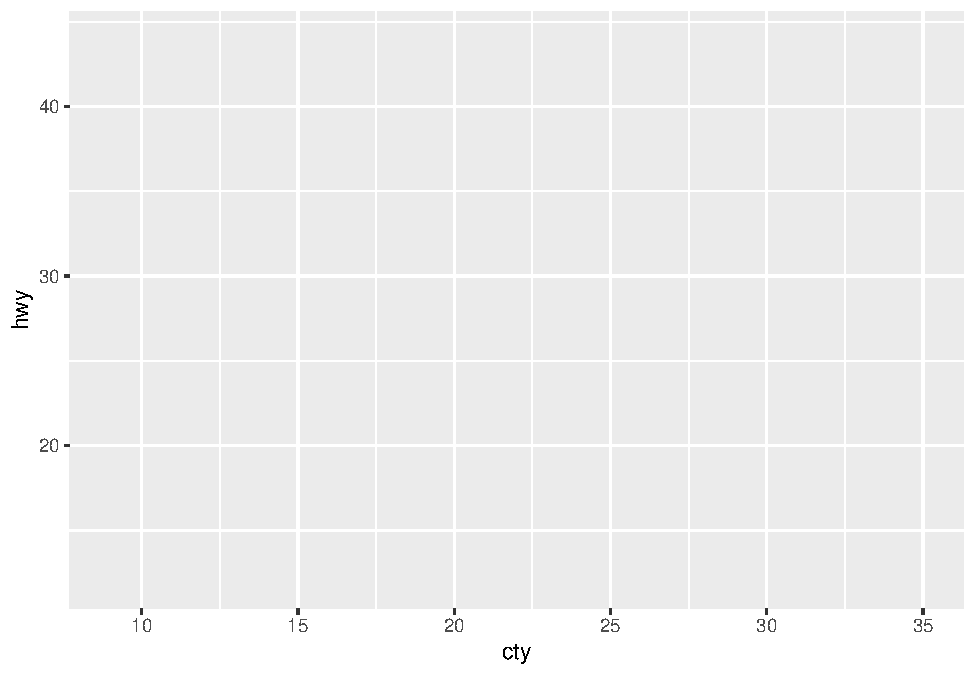
\includegraphics{02_ggplot2_files/figure-latex/unnamed-chunk-3-2.pdf}

\begin{Shaded}
\begin{Highlighting}[]
\CommentTok{\# Alternativas}
\FunctionTok{ggplot}\NormalTok{(dados, }\FunctionTok{aes}\NormalTok{(}\AttributeTok{x =}\NormalTok{ cty, }\AttributeTok{y =}\NormalTok{ hwy)) }\SpecialCharTok{+} 
  \FunctionTok{geom\_point}\NormalTok{()}
\end{Highlighting}
\end{Shaded}

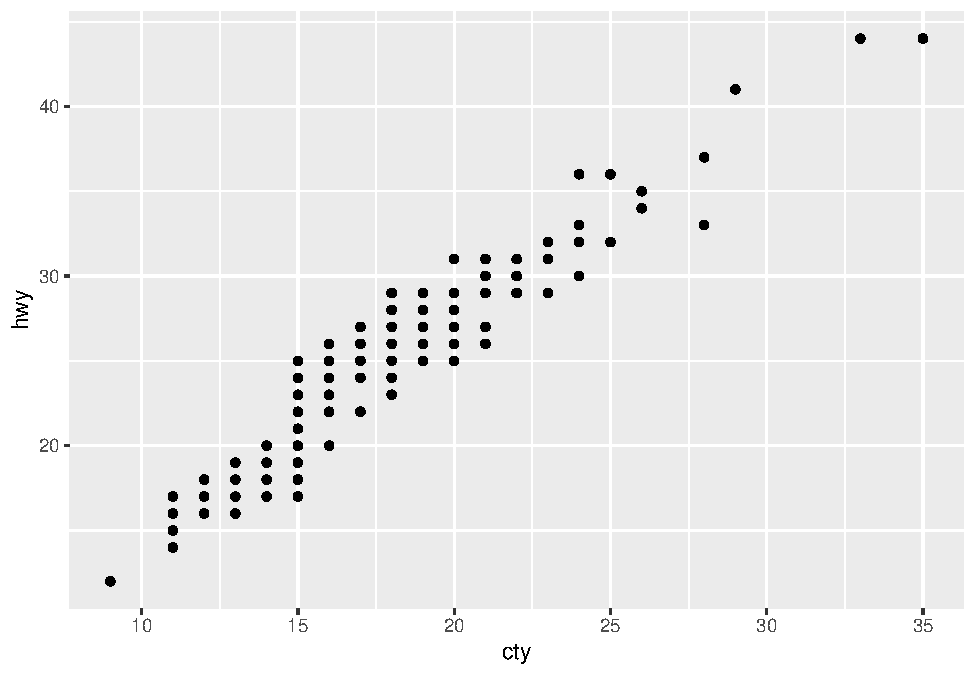
\includegraphics{02_ggplot2_files/figure-latex/unnamed-chunk-3-3.pdf}

\begin{Shaded}
\begin{Highlighting}[]
\FunctionTok{ggplot}\NormalTok{(dados) }\SpecialCharTok{+} 
  \FunctionTok{geom\_point}\NormalTok{(}\FunctionTok{aes}\NormalTok{(}\AttributeTok{x =}\NormalTok{ cty, }\AttributeTok{y =}\NormalTok{ hwy))}
\end{Highlighting}
\end{Shaded}

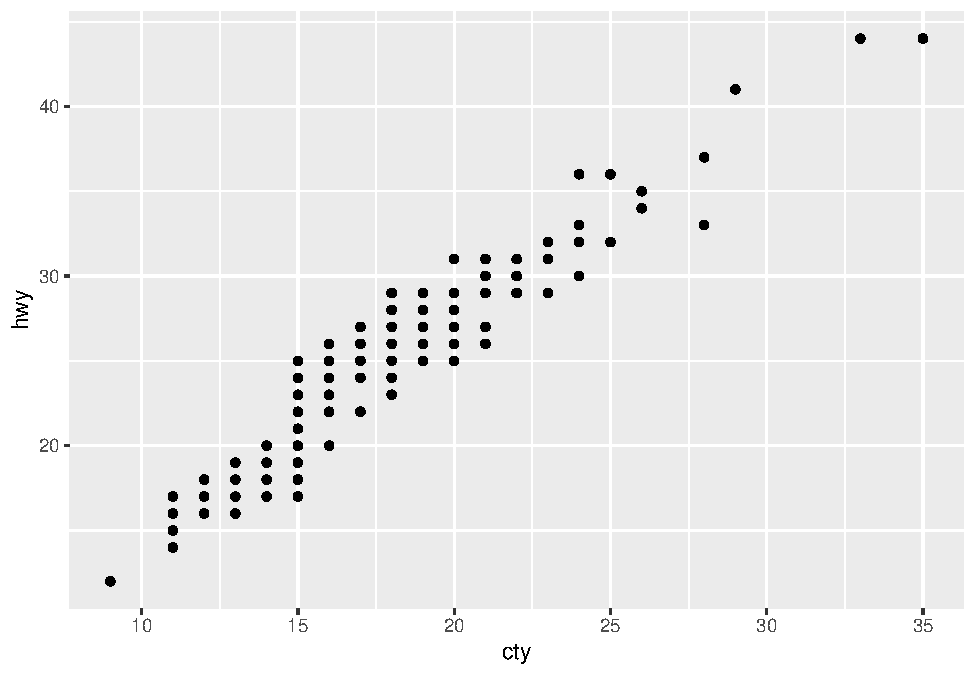
\includegraphics{02_ggplot2_files/figure-latex/unnamed-chunk-3-4.pdf}

\begin{Shaded}
\begin{Highlighting}[]
\FunctionTok{ggplot}\NormalTok{() }\SpecialCharTok{+} 
  \FunctionTok{geom\_point}\NormalTok{(}\AttributeTok{data =}\NormalTok{ dados, }\FunctionTok{aes}\NormalTok{(}\AttributeTok{x =}\NormalTok{ cty, }\AttributeTok{y =}\NormalTok{ hwy))}
\end{Highlighting}
\end{Shaded}

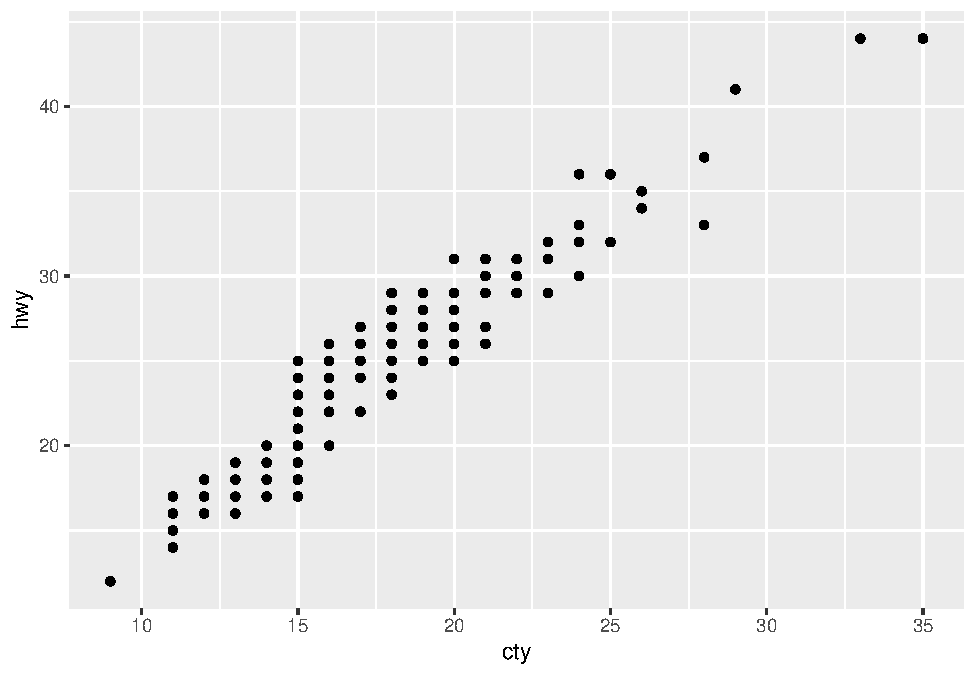
\includegraphics{02_ggplot2_files/figure-latex/unnamed-chunk-3-5.pdf}

\begin{Shaded}
\begin{Highlighting}[]
\CommentTok{\# Fim }

\FunctionTok{ggplot}\NormalTok{(dados, }\FunctionTok{aes}\NormalTok{(}\AttributeTok{x =}\NormalTok{ cty, }\AttributeTok{y =}\NormalTok{ hwy)) }\SpecialCharTok{+} 
  \FunctionTok{geom\_point}\NormalTok{(}\AttributeTok{colour =} \StringTok{"red"}\NormalTok{)}
\end{Highlighting}
\end{Shaded}

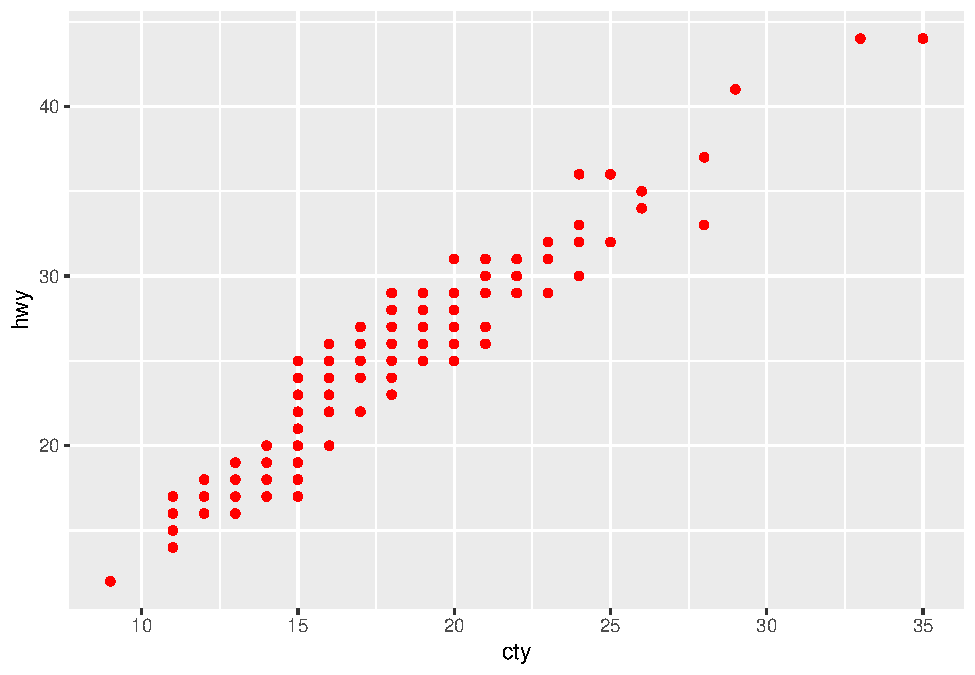
\includegraphics{02_ggplot2_files/figure-latex/unnamed-chunk-3-6.pdf}

\begin{Shaded}
\begin{Highlighting}[]
\FunctionTok{ggplot}\NormalTok{(dados, }\FunctionTok{aes}\NormalTok{(}\AttributeTok{x =}\NormalTok{ cty, }\AttributeTok{y =}\NormalTok{ hwy)) }\SpecialCharTok{+} 
  \FunctionTok{geom\_point}\NormalTok{(}\AttributeTok{colour =} \StringTok{"red"}\NormalTok{, }\AttributeTok{size =} \DecValTok{6}\NormalTok{)}
\end{Highlighting}
\end{Shaded}

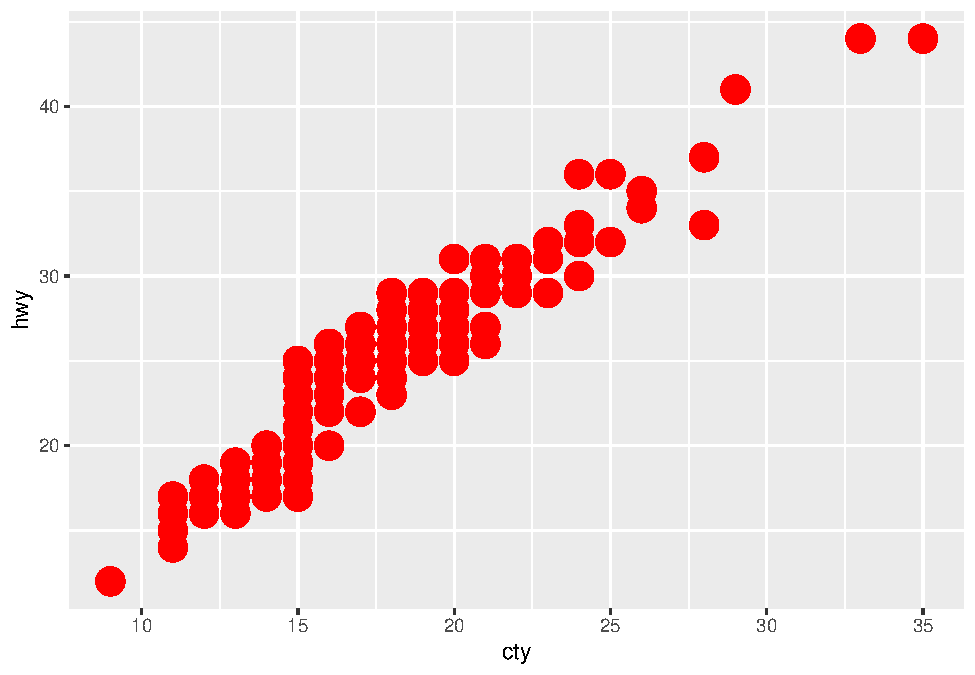
\includegraphics{02_ggplot2_files/figure-latex/unnamed-chunk-3-7.pdf}

\begin{Shaded}
\begin{Highlighting}[]
\FunctionTok{ggplot}\NormalTok{(dados, }\FunctionTok{aes}\NormalTok{(}\AttributeTok{x =}\NormalTok{ cty, }\AttributeTok{y =}\NormalTok{ hwy)) }\SpecialCharTok{+} 
  \FunctionTok{geom\_point}\NormalTok{(}\AttributeTok{colour =} \StringTok{"red"}\NormalTok{, }\AttributeTok{size =} \DecValTok{6}\NormalTok{, }\AttributeTok{shape =} \DecValTok{10}\NormalTok{)}
\end{Highlighting}
\end{Shaded}

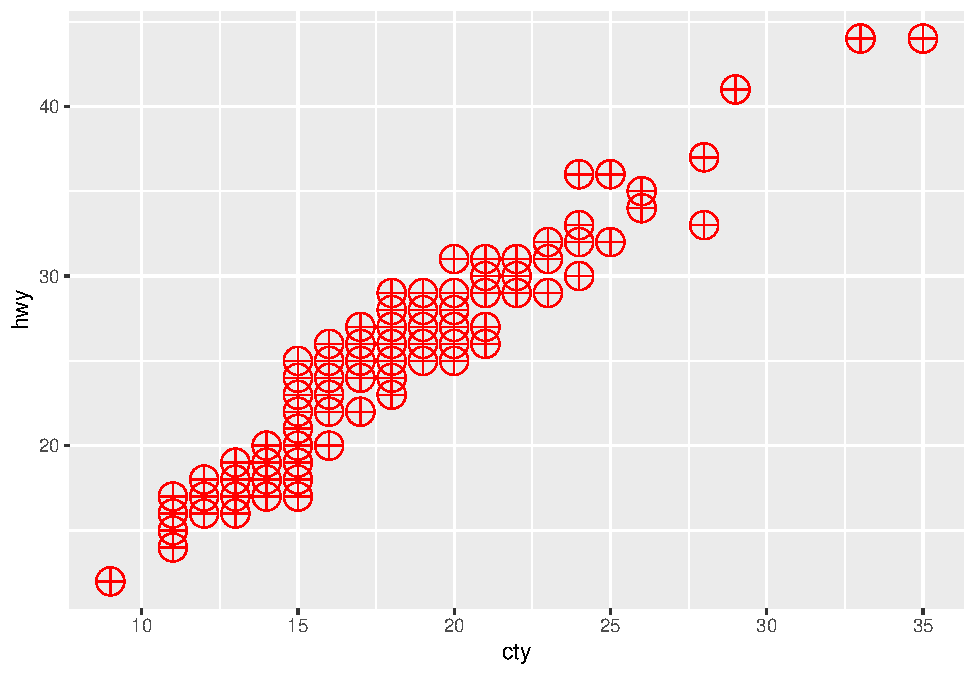
\includegraphics{02_ggplot2_files/figure-latex/unnamed-chunk-3-8.pdf}

\begin{Shaded}
\begin{Highlighting}[]
\CommentTok{\# Alternativa}
\FunctionTok{ggplot}\NormalTok{(dados, }\FunctionTok{aes}\NormalTok{(}\AttributeTok{x =}\NormalTok{ cty, }\AttributeTok{y =}\NormalTok{ hwy)) }\SpecialCharTok{+} 
  \FunctionTok{geom\_point}\NormalTok{(}\AttributeTok{colour =} \StringTok{"red"}\NormalTok{, }\AttributeTok{size =} \DecValTok{6}\NormalTok{, }\AttributeTok{shape =} \StringTok{"circle plus"}\NormalTok{)}
\end{Highlighting}
\end{Shaded}

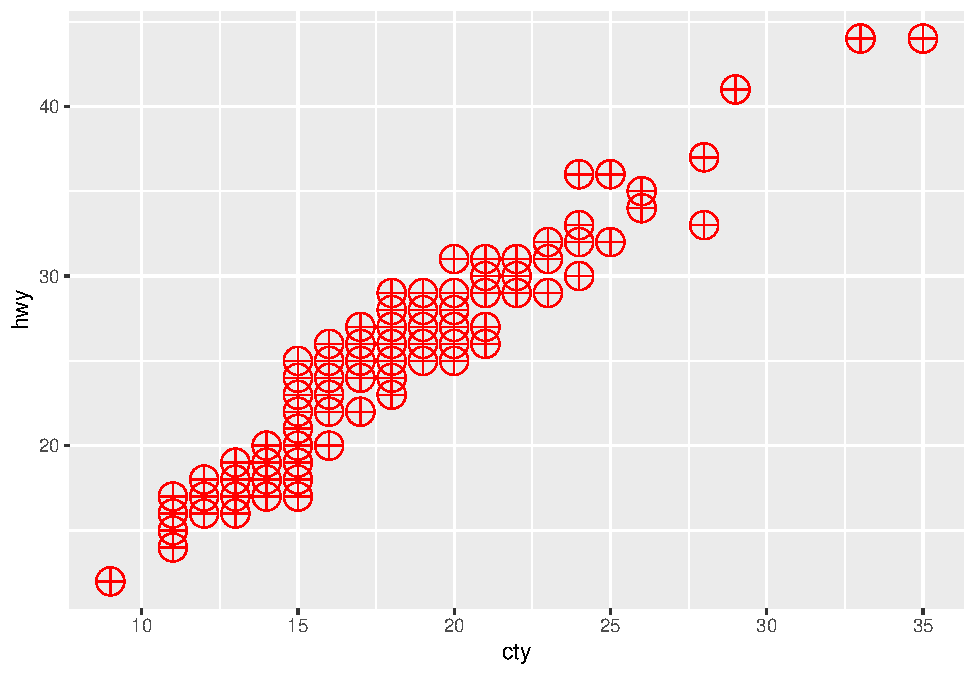
\includegraphics{02_ggplot2_files/figure-latex/unnamed-chunk-3-9.pdf}

\begin{Shaded}
\begin{Highlighting}[]
\FunctionTok{ggplot}\NormalTok{(dados, }\FunctionTok{aes}\NormalTok{(}\AttributeTok{x =}\NormalTok{ cty, }\AttributeTok{y =}\NormalTok{ hwy)) }\SpecialCharTok{+} 
  \FunctionTok{geom\_point}\NormalTok{(}\AttributeTok{colour =} \StringTok{"red"}\NormalTok{, }\AttributeTok{size =} \DecValTok{6}\NormalTok{, }\AttributeTok{shape =} \DecValTok{10}\NormalTok{)}\SpecialCharTok{+}
  \FunctionTok{labs}\NormalTok{(}\AttributeTok{x =} \StringTok{"cty (city miles per gallon hwy)"}\NormalTok{, }
       \AttributeTok{y =} \StringTok{"hwy (highway miles per gallon)"}\NormalTok{, }
       \AttributeTok{title =} \StringTok{"Pensar em algum título..."}\NormalTok{, }
       \AttributeTok{subtitle =} \StringTok{"Escrever alguma coisa"}\NormalTok{)}
\end{Highlighting}
\end{Shaded}

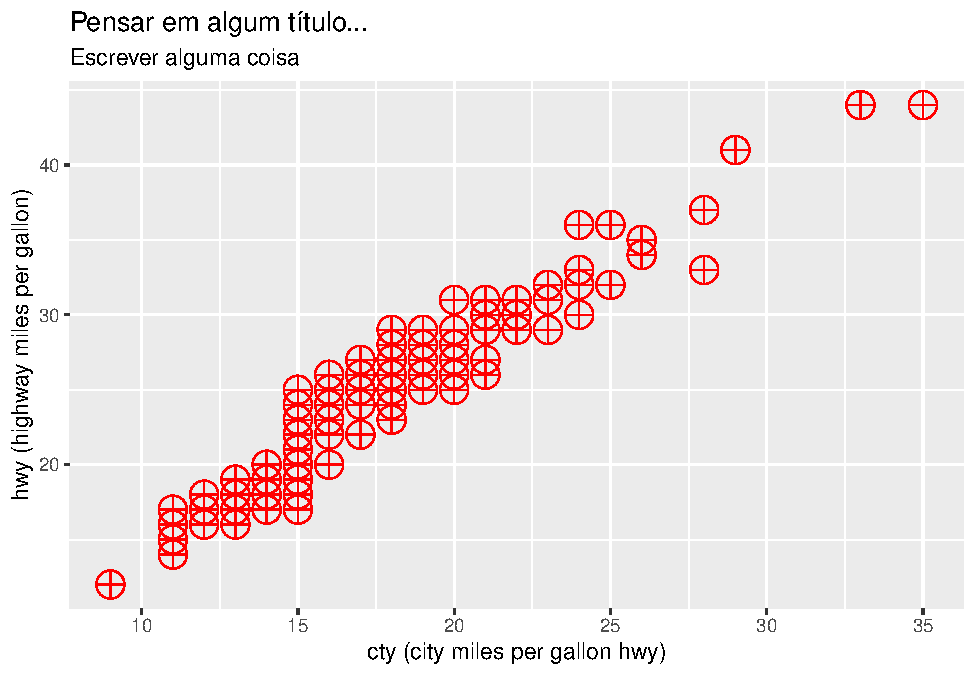
\includegraphics{02_ggplot2_files/figure-latex/unnamed-chunk-3-10.pdf}

\hypertarget{mais-detalhes-sobre-geom_point}{%
\subsection{Mais detalhes sobre geom\_point}\label{mais-detalhes-sobre-geom_point}}

\begin{quote}
geom\_point() understands the following aesthetics (required aesthetics are in bold):
\end{quote}

\begin{itemize}
\item
  x
\item
  y
\item
  alpha
\item
  colour
\item
  fill
\item
  group
\item
  shape
\item
  size
\item
  stroke
\end{itemize}

\begin{Shaded}
\begin{Highlighting}[]
\FunctionTok{ggplot}\NormalTok{(dados, }\FunctionTok{aes}\NormalTok{(}\AttributeTok{x =}\NormalTok{ cty, }\AttributeTok{y =}\NormalTok{ hwy)) }\SpecialCharTok{+} 
  \FunctionTok{geom\_point}\NormalTok{()}
\end{Highlighting}
\end{Shaded}

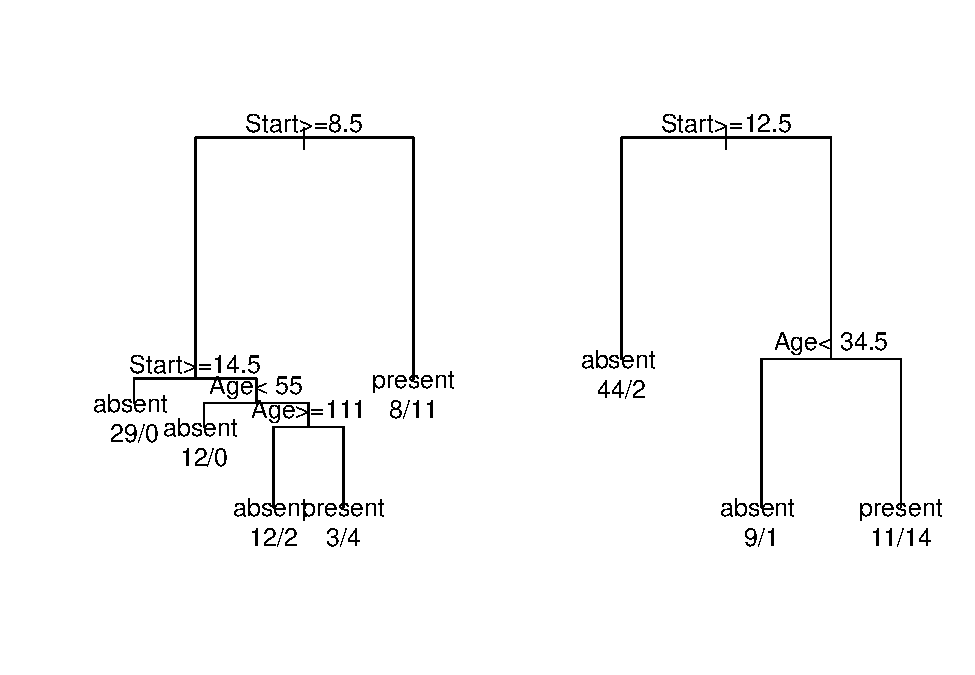
\includegraphics{02_ggplot2_files/figure-latex/unnamed-chunk-4-1.pdf}

\begin{Shaded}
\begin{Highlighting}[]
\FunctionTok{ggplot}\NormalTok{(dados, }\FunctionTok{aes}\NormalTok{(}\AttributeTok{x =}\NormalTok{ cty, }\AttributeTok{y =}\NormalTok{ hwy, }\AttributeTok{col =} \FunctionTok{factor}\NormalTok{(year))) }\SpecialCharTok{+} 
  \FunctionTok{geom\_point}\NormalTok{() }\SpecialCharTok{+} 
  \FunctionTok{labs}\NormalTok{(}\AttributeTok{col =} \StringTok{"year"}\NormalTok{)}
\end{Highlighting}
\end{Shaded}

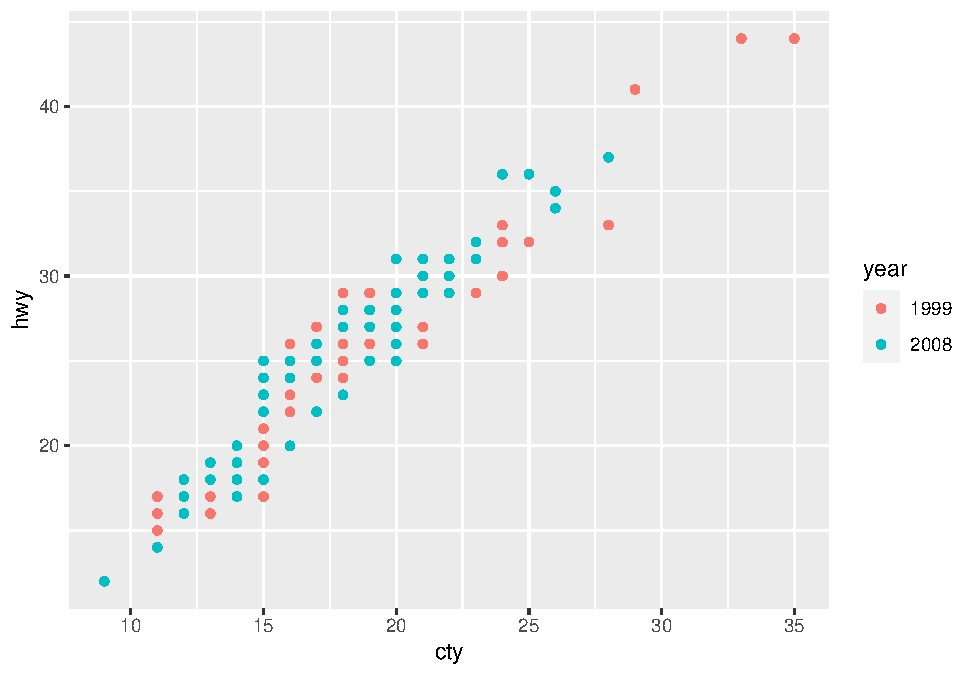
\includegraphics{02_ggplot2_files/figure-latex/unnamed-chunk-4-2.pdf}

\begin{Shaded}
\begin{Highlighting}[]
\CommentTok{\# Alternativa}
\FunctionTok{ggplot}\NormalTok{(dados, }\FunctionTok{aes}\NormalTok{(}\AttributeTok{x =}\NormalTok{ cty, }\AttributeTok{y =}\NormalTok{ hwy, }\AttributeTok{col =} \FunctionTok{factor}\NormalTok{(class))) }\SpecialCharTok{+} 
  \FunctionTok{geom\_point}\NormalTok{() }\SpecialCharTok{+} 
  \FunctionTok{labs}\NormalTok{(}\AttributeTok{col =} \StringTok{"class"}\NormalTok{)}\SpecialCharTok{+}
  \FunctionTok{scale\_color\_brewer}\NormalTok{(}\AttributeTok{type =} \StringTok{"qual"}\NormalTok{)}
\end{Highlighting}
\end{Shaded}

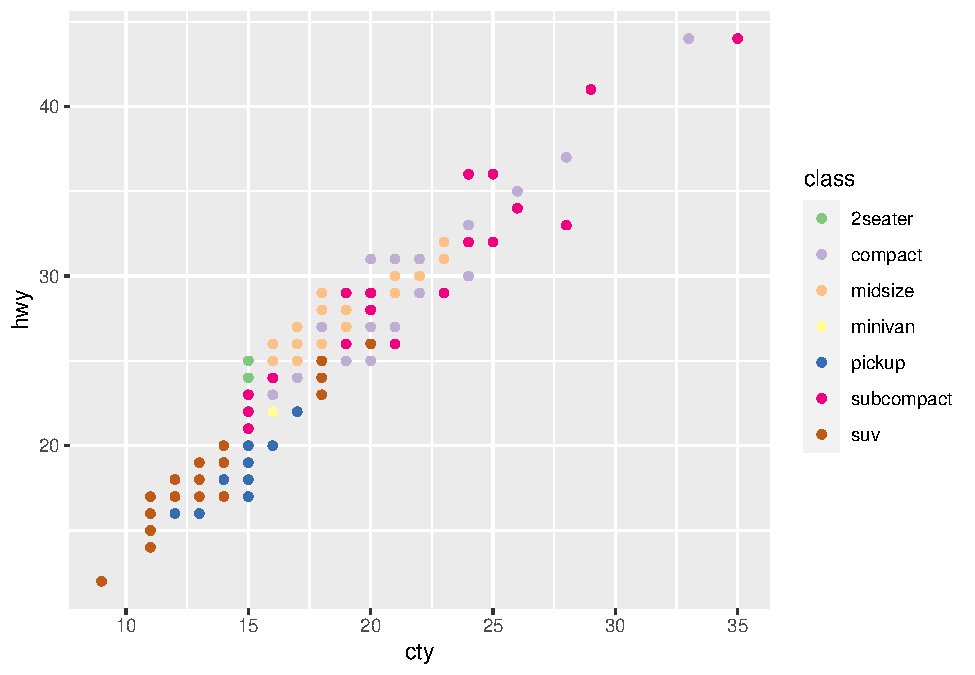
\includegraphics{02_ggplot2_files/figure-latex/unnamed-chunk-4-3.pdf}

\begin{Shaded}
\begin{Highlighting}[]
\FunctionTok{ggplot}\NormalTok{(dados, }\FunctionTok{aes}\NormalTok{(}\AttributeTok{x =}\NormalTok{ cty, }\AttributeTok{y =}\NormalTok{ hwy, }\AttributeTok{col =} \FunctionTok{factor}\NormalTok{(class))) }\SpecialCharTok{+} 
  \FunctionTok{geom\_point}\NormalTok{() }\SpecialCharTok{+} 
  \FunctionTok{labs}\NormalTok{(}\AttributeTok{col =} \StringTok{"class"}\NormalTok{)}\SpecialCharTok{+}
  \FunctionTok{scale\_color\_brewer}\NormalTok{(}\AttributeTok{type =} \StringTok{"div"}\NormalTok{)}
\end{Highlighting}
\end{Shaded}

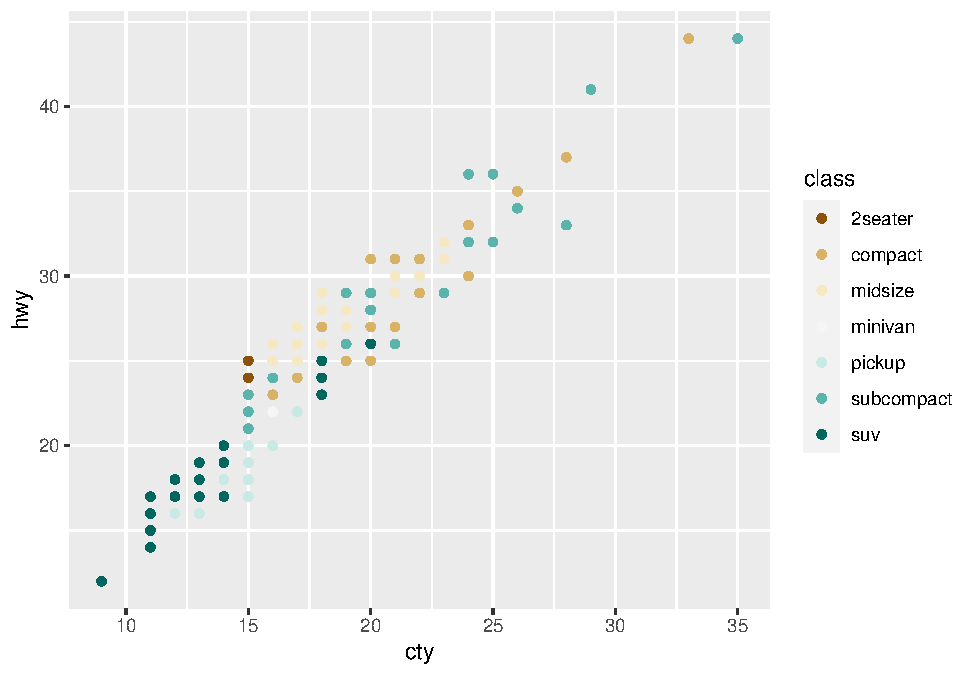
\includegraphics{02_ggplot2_files/figure-latex/unnamed-chunk-4-4.pdf}

\begin{Shaded}
\begin{Highlighting}[]
\FunctionTok{ggplot}\NormalTok{(dados, }\FunctionTok{aes}\NormalTok{(}\AttributeTok{x =}\NormalTok{ cty, }\AttributeTok{y =}\NormalTok{ hwy, }\AttributeTok{col =} \FunctionTok{factor}\NormalTok{(class))) }\SpecialCharTok{+} 
  \FunctionTok{geom\_point}\NormalTok{() }\SpecialCharTok{+} 
  \FunctionTok{labs}\NormalTok{(}\AttributeTok{col =} \StringTok{"class"}\NormalTok{)}\SpecialCharTok{+}
  \FunctionTok{scale\_color\_brewer}\NormalTok{(}\AttributeTok{palette =} \StringTok{"Set1"}\NormalTok{, }\AttributeTok{name =} \StringTok{"Tipo de carro"}\NormalTok{)}\SpecialCharTok{+}
  \FunctionTok{scale\_y\_continuous}\NormalTok{(}\AttributeTok{breaks =} \FunctionTok{seq}\NormalTok{(}\DecValTok{10}\NormalTok{,}\DecValTok{60}\NormalTok{,}\DecValTok{3}\NormalTok{))}\SpecialCharTok{+}
  \FunctionTok{scale\_x\_continuous}\NormalTok{(}\AttributeTok{breaks =} \FunctionTok{seq}\NormalTok{(}\DecValTok{10}\NormalTok{,}\DecValTok{40}\NormalTok{,}\DecValTok{3}\NormalTok{))}\SpecialCharTok{+}
  \FunctionTok{theme\_minimal}\NormalTok{()}
\end{Highlighting}
\end{Shaded}

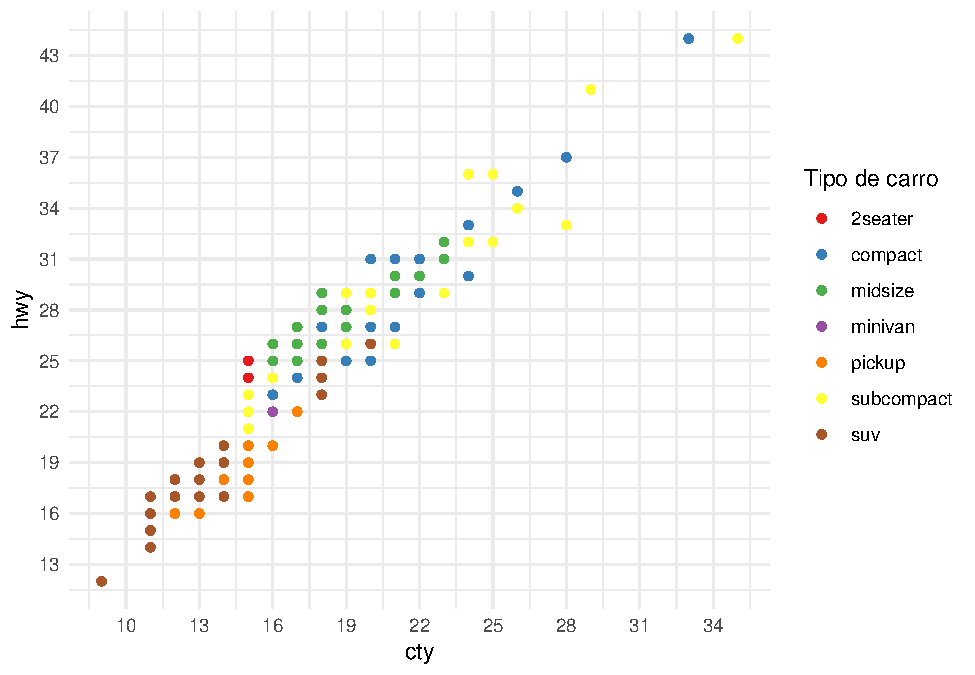
\includegraphics{02_ggplot2_files/figure-latex/unnamed-chunk-4-5.pdf}

\begin{Shaded}
\begin{Highlighting}[]
\FunctionTok{ggplot}\NormalTok{(dados, }\FunctionTok{aes}\NormalTok{(}\AttributeTok{x =}\NormalTok{ cty, }\AttributeTok{y =}\NormalTok{ hwy, }\AttributeTok{alpha =} \FunctionTok{factor}\NormalTok{(year))) }\SpecialCharTok{+} 
  \FunctionTok{geom\_point}\NormalTok{() }\SpecialCharTok{+} 
  \FunctionTok{labs}\NormalTok{(}\AttributeTok{alpha =} \StringTok{"year"}\NormalTok{)}
\end{Highlighting}
\end{Shaded}

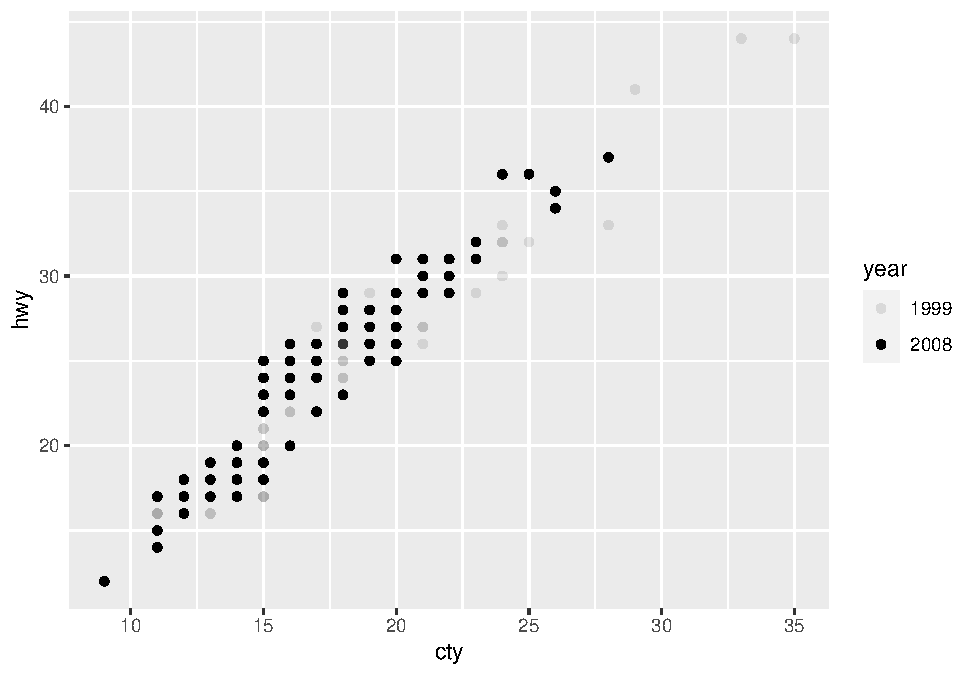
\includegraphics{02_ggplot2_files/figure-latex/unnamed-chunk-4-6.pdf}

\begin{Shaded}
\begin{Highlighting}[]
\FunctionTok{ggplot}\NormalTok{(dados, }\FunctionTok{aes}\NormalTok{(}\AttributeTok{x =}\NormalTok{ cty, }\AttributeTok{y =}\NormalTok{ hwy, }\AttributeTok{size =} \FunctionTok{factor}\NormalTok{(year))) }\SpecialCharTok{+} 
  \FunctionTok{geom\_point}\NormalTok{() }\SpecialCharTok{+} 
  \FunctionTok{labs}\NormalTok{(}\AttributeTok{size =} \StringTok{"year"}\NormalTok{)}
\end{Highlighting}
\end{Shaded}

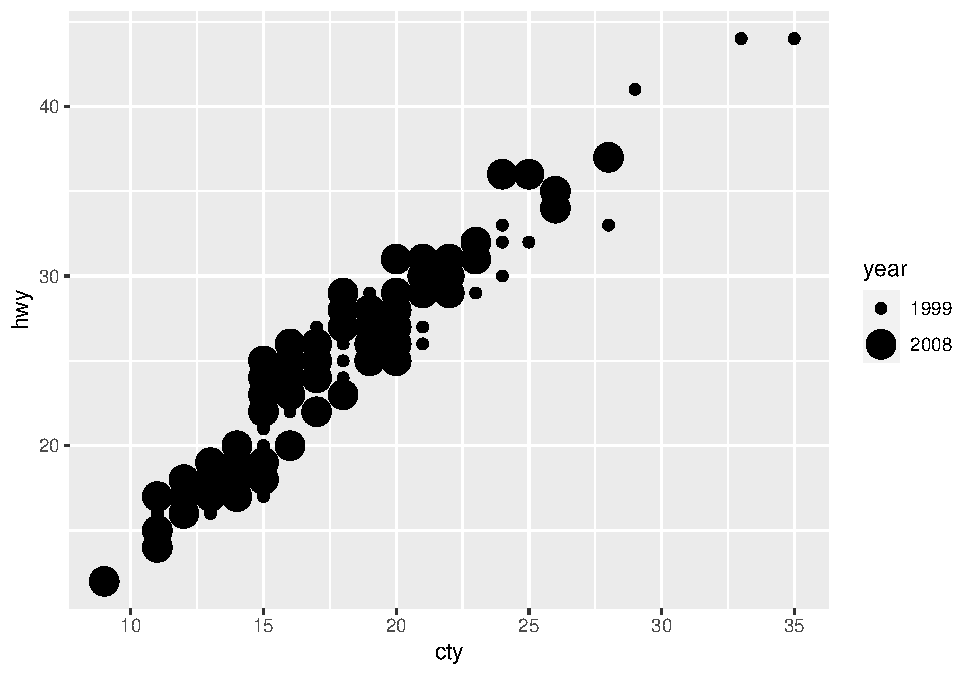
\includegraphics{02_ggplot2_files/figure-latex/unnamed-chunk-4-7.pdf}

\begin{Shaded}
\begin{Highlighting}[]
\CommentTok{\# Alternativa}
\FunctionTok{ggplot}\NormalTok{(dados, }\FunctionTok{aes}\NormalTok{(}\AttributeTok{x =}\NormalTok{ cty, }\AttributeTok{y =}\NormalTok{ hwy, }\AttributeTok{col =}\NormalTok{ cty }\SpecialCharTok{\textless{}=} \DecValTok{20}\NormalTok{)) }\SpecialCharTok{+} 
  \FunctionTok{geom\_point}\NormalTok{() }\SpecialCharTok{+} 
  \FunctionTok{geom\_vline}\NormalTok{(}\AttributeTok{xintercept =} \DecValTok{20}\NormalTok{)}\SpecialCharTok{+}
  \FunctionTok{labs}\NormalTok{(}\AttributeTok{col =} \StringTok{"year"}\NormalTok{)}
\end{Highlighting}
\end{Shaded}

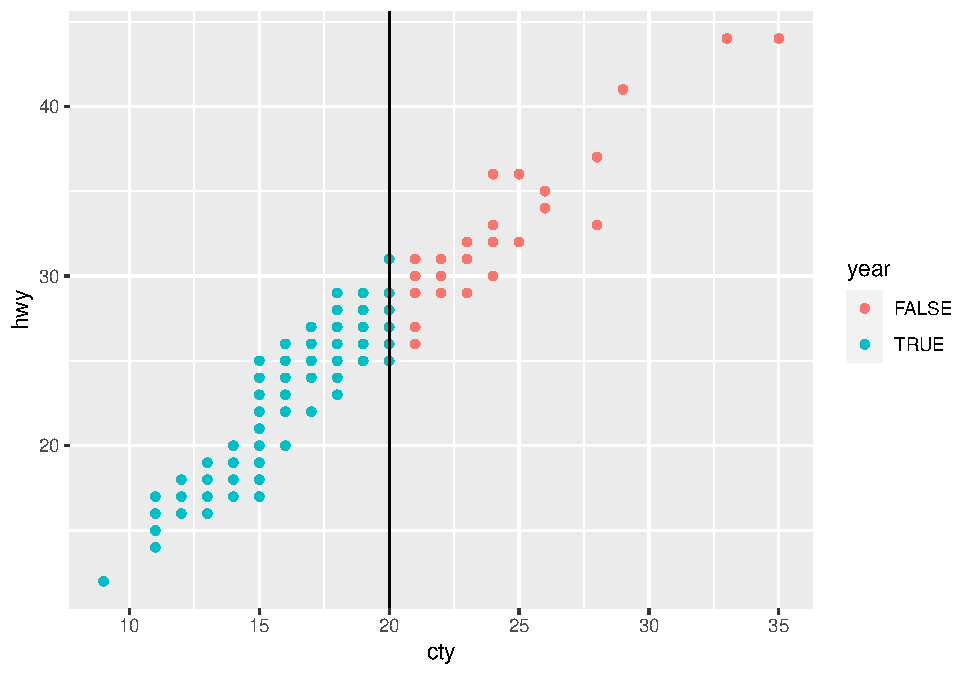
\includegraphics{02_ggplot2_files/figure-latex/unnamed-chunk-4-8.pdf}

\begin{Shaded}
\begin{Highlighting}[]
\CommentTok{\# Erro comum}
\FunctionTok{ggplot}\NormalTok{(dados, }\FunctionTok{aes}\NormalTok{(}\AttributeTok{x =}\NormalTok{ cty, }\AttributeTok{y =}\NormalTok{ hwy, }\AttributeTok{col =} \StringTok{"red"}\NormalTok{)) }\SpecialCharTok{+} 
  \FunctionTok{geom\_point}\NormalTok{()}\SpecialCharTok{+}
  \FunctionTok{labs}\NormalTok{(}\AttributeTok{col =} \StringTok{"year"}\NormalTok{)}
\end{Highlighting}
\end{Shaded}

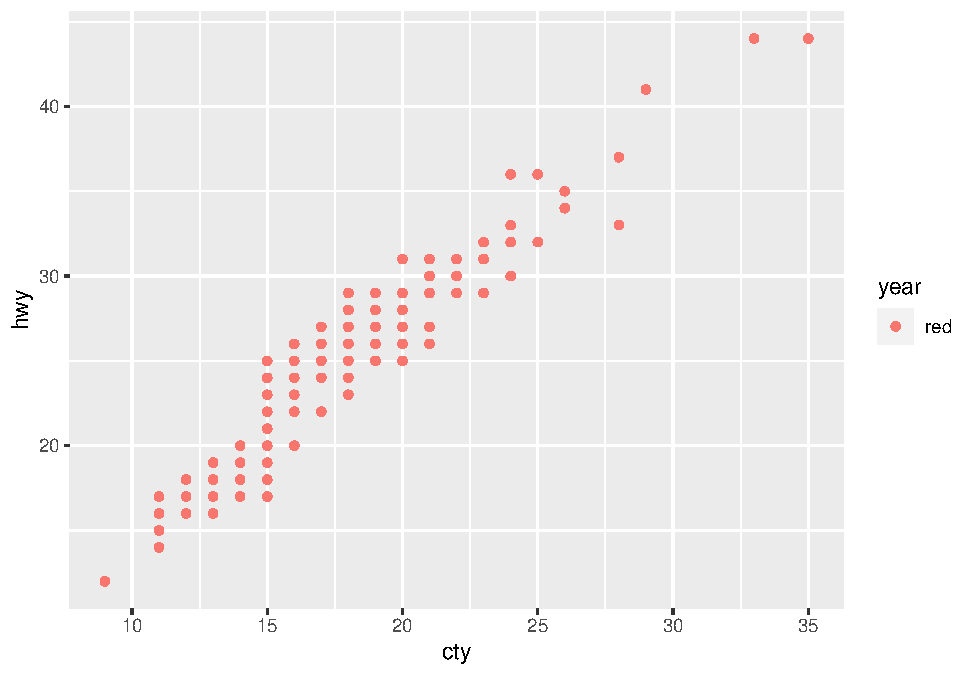
\includegraphics{02_ggplot2_files/figure-latex/unnamed-chunk-4-9.pdf}

\begin{Shaded}
\begin{Highlighting}[]
\FunctionTok{ggplot}\NormalTok{(dados, }\FunctionTok{aes}\NormalTok{(}\AttributeTok{x =}\NormalTok{ cty, }\AttributeTok{y =}\NormalTok{ hwy)) }\SpecialCharTok{+} 
  \FunctionTok{geom\_point}\NormalTok{(}\AttributeTok{col =} \StringTok{"red"}\NormalTok{)}\SpecialCharTok{+}
  \FunctionTok{labs}\NormalTok{(}\AttributeTok{col =} \StringTok{"year"}\NormalTok{)}
\end{Highlighting}
\end{Shaded}

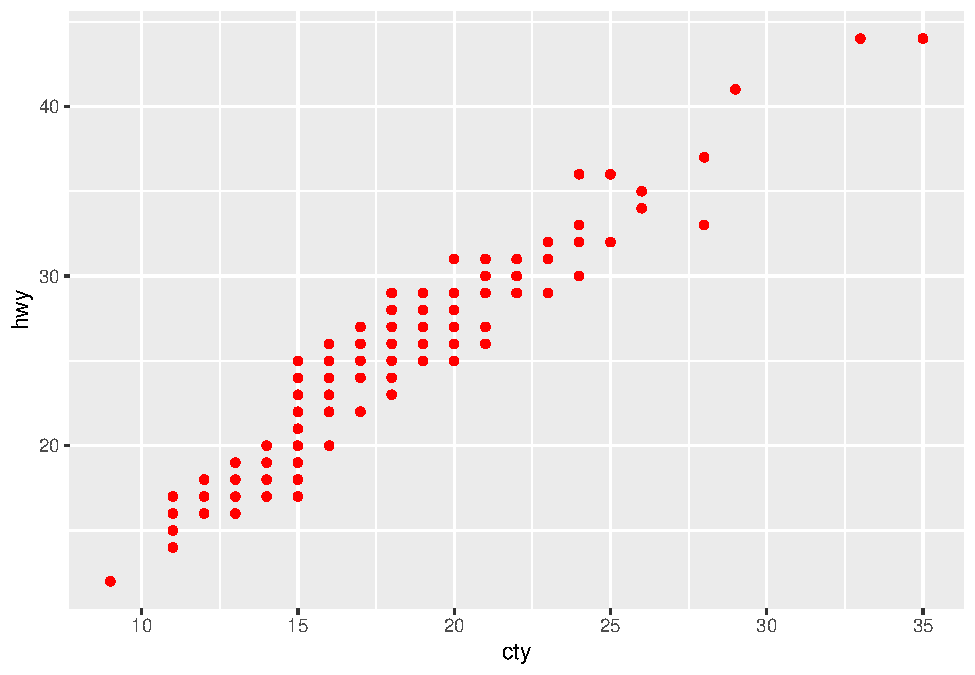
\includegraphics{02_ggplot2_files/figure-latex/unnamed-chunk-4-10.pdf}

\begin{Shaded}
\begin{Highlighting}[]
\CommentTok{\# Fim  Erro comum}

\FunctionTok{ggplot}\NormalTok{(dados, }\FunctionTok{aes}\NormalTok{(}\AttributeTok{x =}\NormalTok{ cty, }\AttributeTok{y =}\NormalTok{ hwy, }\AttributeTok{shape =} \FunctionTok{factor}\NormalTok{(year))) }\SpecialCharTok{+} 
  \FunctionTok{geom\_point}\NormalTok{(}\AttributeTok{col =} \StringTok{"red"}\NormalTok{) }\SpecialCharTok{+} 
  \FunctionTok{labs}\NormalTok{(}\AttributeTok{shape =} \StringTok{"year"}\NormalTok{)}
\end{Highlighting}
\end{Shaded}

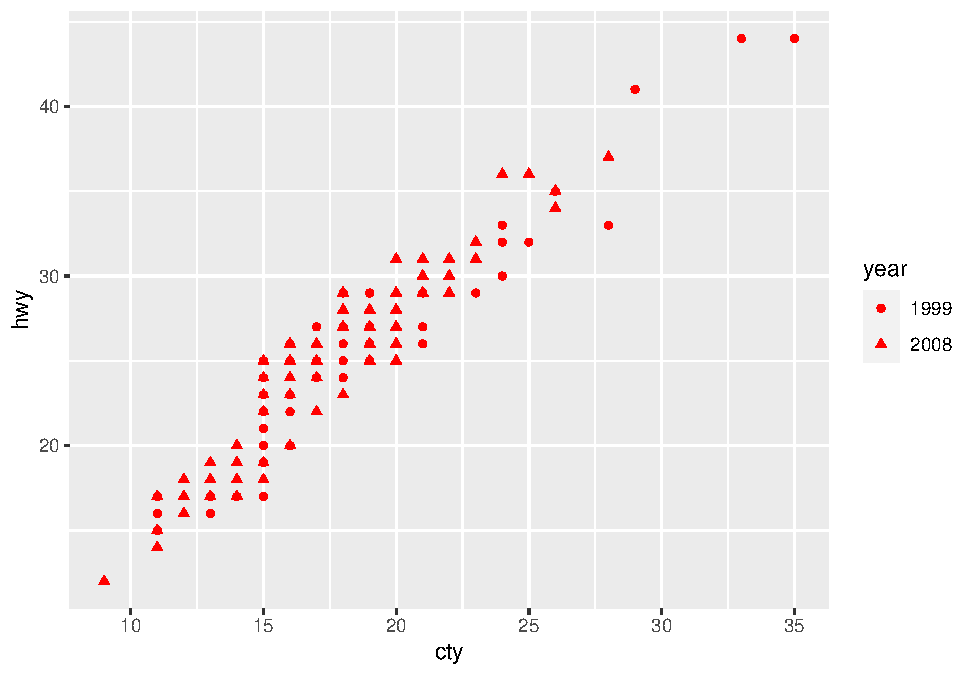
\includegraphics{02_ggplot2_files/figure-latex/unnamed-chunk-4-11.pdf}

\begin{Shaded}
\begin{Highlighting}[]
\FunctionTok{ggplot}\NormalTok{(dados, }\FunctionTok{aes}\NormalTok{(}\AttributeTok{x =}\NormalTok{ cty, }\AttributeTok{y =}\NormalTok{ hwy, }\AttributeTok{size =}\NormalTok{ class)) }\SpecialCharTok{+} 
  \FunctionTok{geom\_point}\NormalTok{() }\SpecialCharTok{+} 
  \FunctionTok{labs}\NormalTok{(}\AttributeTok{size =} \StringTok{"class"}\NormalTok{)}
\end{Highlighting}
\end{Shaded}

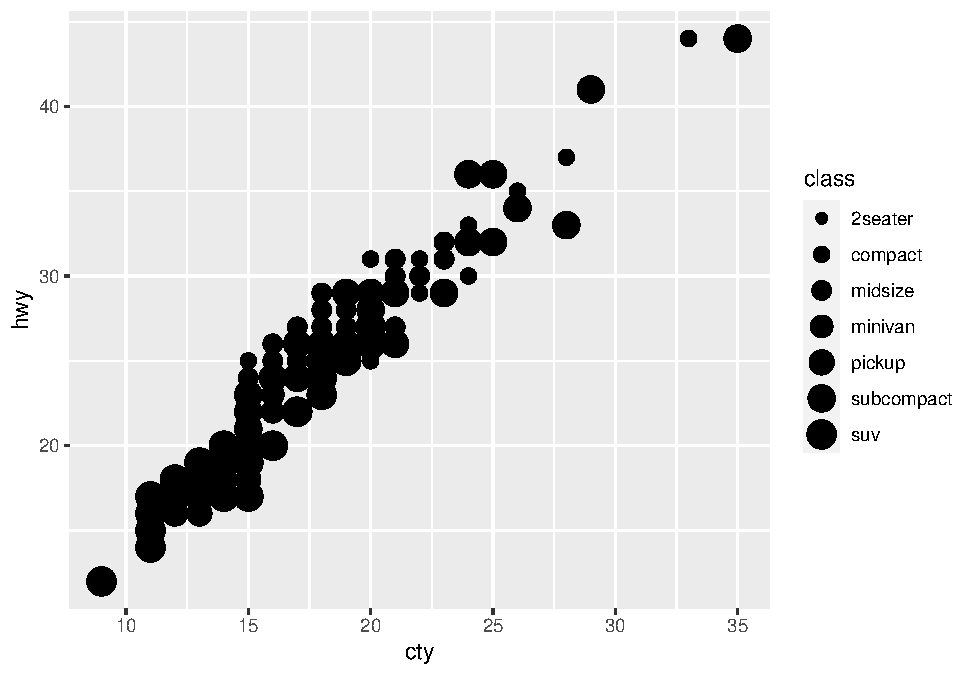
\includegraphics{02_ggplot2_files/figure-latex/unnamed-chunk-4-12.pdf}

\begin{Shaded}
\begin{Highlighting}[]
\FunctionTok{ggplot}\NormalTok{(dados, }\FunctionTok{aes}\NormalTok{(}\AttributeTok{x =}\NormalTok{ cty, }\AttributeTok{y =}\NormalTok{ hwy, }
                  \AttributeTok{size =}\NormalTok{ class, }
                  \AttributeTok{col =}\NormalTok{ class)) }\SpecialCharTok{+} 
  \FunctionTok{geom\_point}\NormalTok{() }\SpecialCharTok{+} 
  \FunctionTok{guides}\NormalTok{(}\AttributeTok{colour =} \FunctionTok{guide\_legend}\NormalTok{(}\StringTok{"Tipo de carro (color)"}\NormalTok{),}
         \AttributeTok{size =} \FunctionTok{guide\_legend}\NormalTok{(}\StringTok{"Tipo de carro (size)"}\NormalTok{))}
\end{Highlighting}
\end{Shaded}

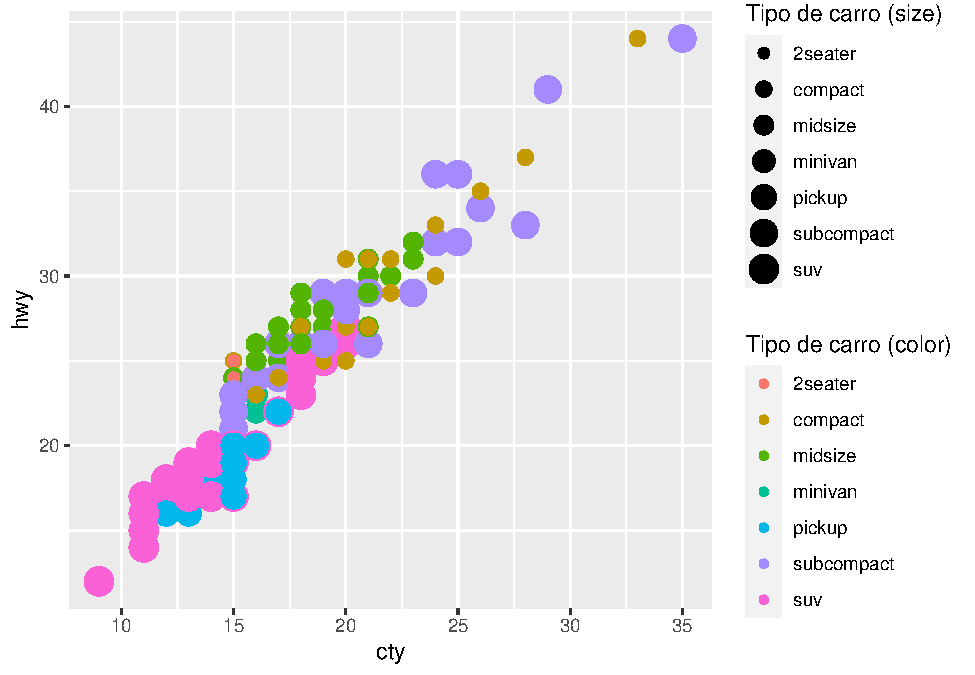
\includegraphics{02_ggplot2_files/figure-latex/unnamed-chunk-4-13.pdf}

\begin{Shaded}
\begin{Highlighting}[]
\FunctionTok{ggplot}\NormalTok{(dados, }\FunctionTok{aes}\NormalTok{(}\AttributeTok{x =}\NormalTok{ cty, }\AttributeTok{y =}\NormalTok{ hwy, }
                  \AttributeTok{size =}\NormalTok{ class, }
                  \AttributeTok{col =}\NormalTok{ class)) }\SpecialCharTok{+} 
  \FunctionTok{geom\_point}\NormalTok{() }\SpecialCharTok{+} 
  \FunctionTok{labs}\NormalTok{(}\AttributeTok{col =} \StringTok{"Tipo de Carro"}\NormalTok{, }\AttributeTok{size =} \StringTok{"Tipo de Carro"}\NormalTok{)}\SpecialCharTok{+}
  \FunctionTok{guides}\NormalTok{(}\AttributeTok{col =} \StringTok{"legend"}\NormalTok{)}
\end{Highlighting}
\end{Shaded}

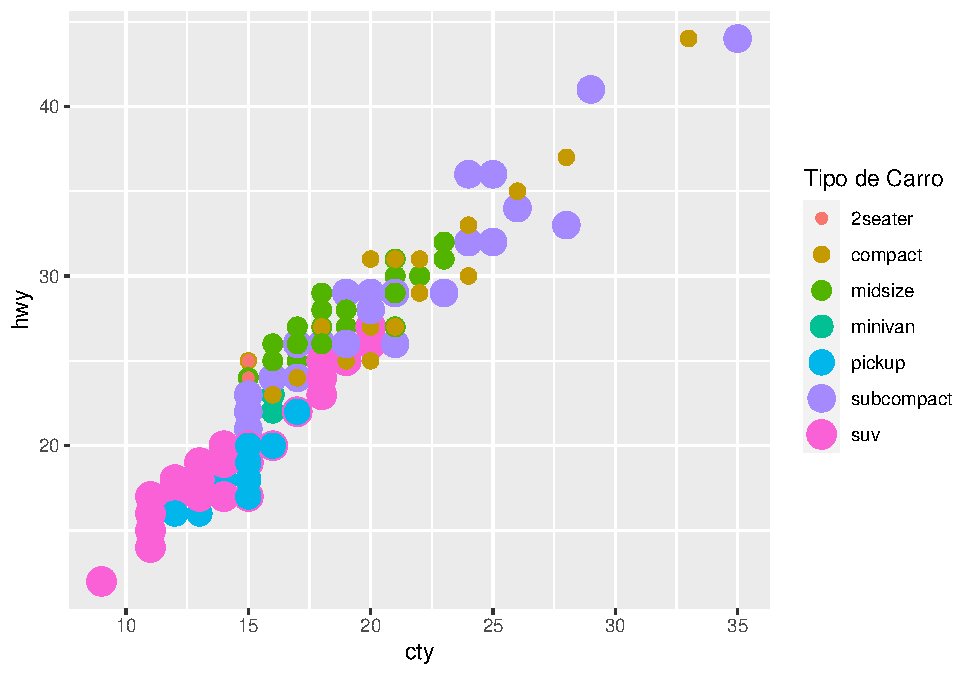
\includegraphics{02_ggplot2_files/figure-latex/unnamed-chunk-4-14.pdf}

\hypertarget{smooth-boxplot-histogram}{%
\section{smooth, boxplot, histogram}\label{smooth-boxplot-histogram}}

\begin{Shaded}
\begin{Highlighting}[]
\NormalTok{v1}\OtherTok{\textless{}{-}} \FunctionTok{ggplot}\NormalTok{(dados, }\FunctionTok{aes}\NormalTok{(}\AttributeTok{x =}\NormalTok{ cty, }\AttributeTok{y =}\NormalTok{ hwy)) }\SpecialCharTok{+} 
  \FunctionTok{geom\_point}\NormalTok{(}\AttributeTok{col =} \StringTok{"blue"}\NormalTok{)}\SpecialCharTok{+}
  \FunctionTok{geom\_smooth}\NormalTok{(}\AttributeTok{method =}\NormalTok{ mgcv}\SpecialCharTok{::}\NormalTok{gam,}
              \AttributeTok{formula =}\NormalTok{ y }\SpecialCharTok{\textasciitilde{}} \FunctionTok{s}\NormalTok{(x, }\AttributeTok{bs =} \StringTok{"cs"}\NormalTok{) ,}
              \AttributeTok{col =} \StringTok{"red"}\NormalTok{, }
              \AttributeTok{se =} \ConstantTok{FALSE}\NormalTok{)}
\NormalTok{v1}
\end{Highlighting}
\end{Shaded}

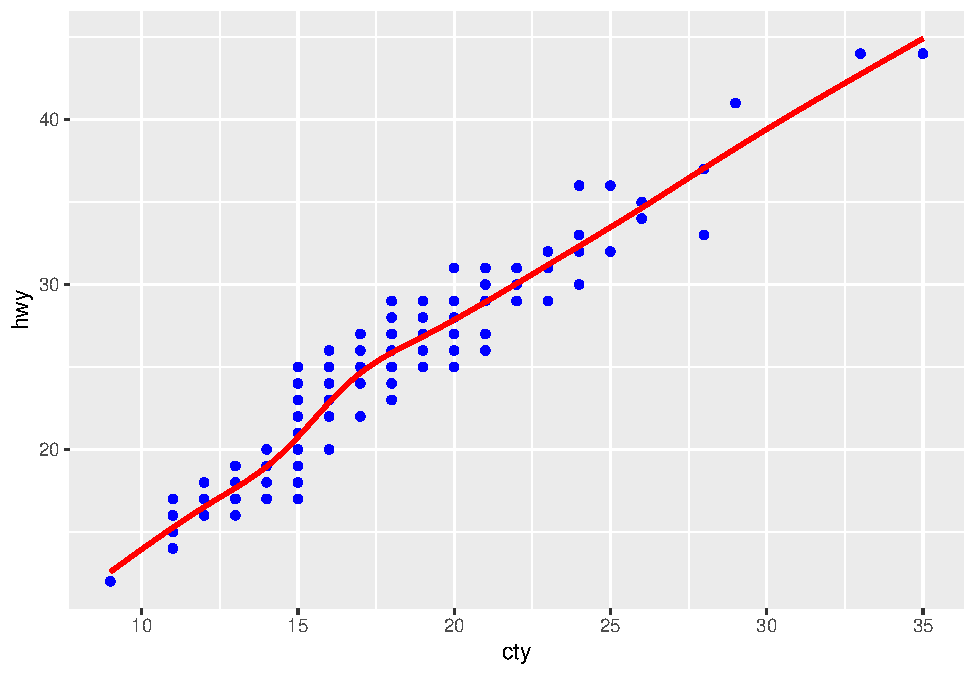
\includegraphics{02_ggplot2_files/figure-latex/unnamed-chunk-5-1.pdf}

\begin{Shaded}
\begin{Highlighting}[]
\NormalTok{v2 }\OtherTok{\textless{}{-}} \FunctionTok{ggplot}\NormalTok{(dados, }\FunctionTok{aes}\NormalTok{(}\AttributeTok{x =}\NormalTok{ cty)) }\SpecialCharTok{+} 
  \FunctionTok{geom\_boxplot}\NormalTok{(}\AttributeTok{fill =} \StringTok{"red"}\NormalTok{)}
\NormalTok{v2}
\end{Highlighting}
\end{Shaded}

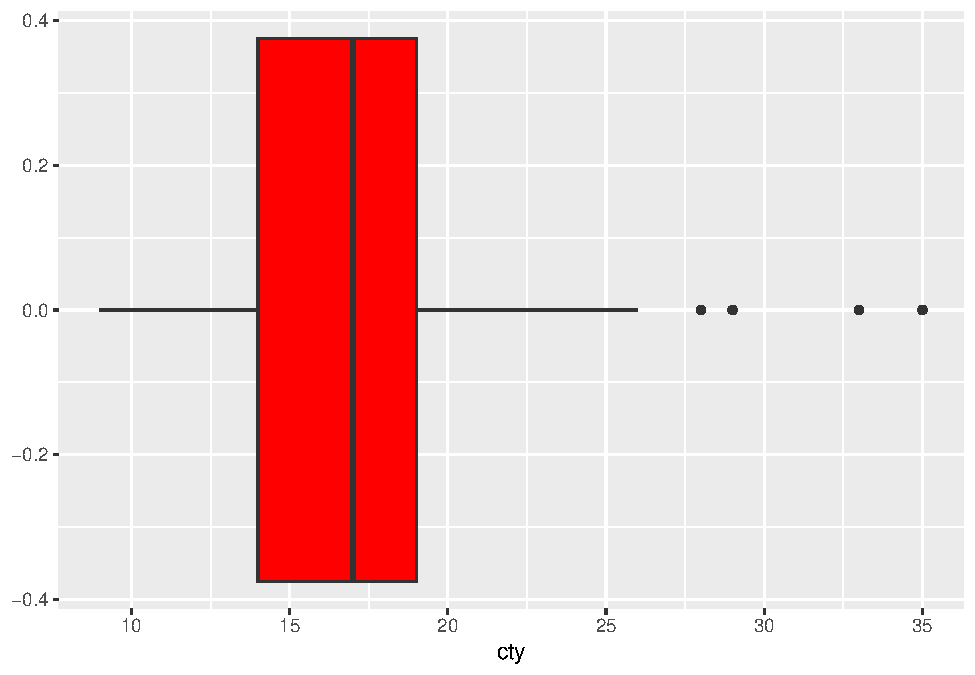
\includegraphics{02_ggplot2_files/figure-latex/unnamed-chunk-5-2.pdf}

\begin{Shaded}
\begin{Highlighting}[]
\NormalTok{v3 }\OtherTok{\textless{}{-}} \FunctionTok{ggplot}\NormalTok{(dados, }\FunctionTok{aes}\NormalTok{(}\AttributeTok{x =}\NormalTok{ cty)) }\SpecialCharTok{+} 
  \FunctionTok{geom\_histogram}\NormalTok{(}\AttributeTok{bins =} \DecValTok{10}\NormalTok{, }\AttributeTok{fill =} \StringTok{"red"}\NormalTok{, }\AttributeTok{col =} \StringTok{"blue"}\NormalTok{, }\AttributeTok{lwd=}\DecValTok{2}\NormalTok{)}
\NormalTok{v3}
\end{Highlighting}
\end{Shaded}

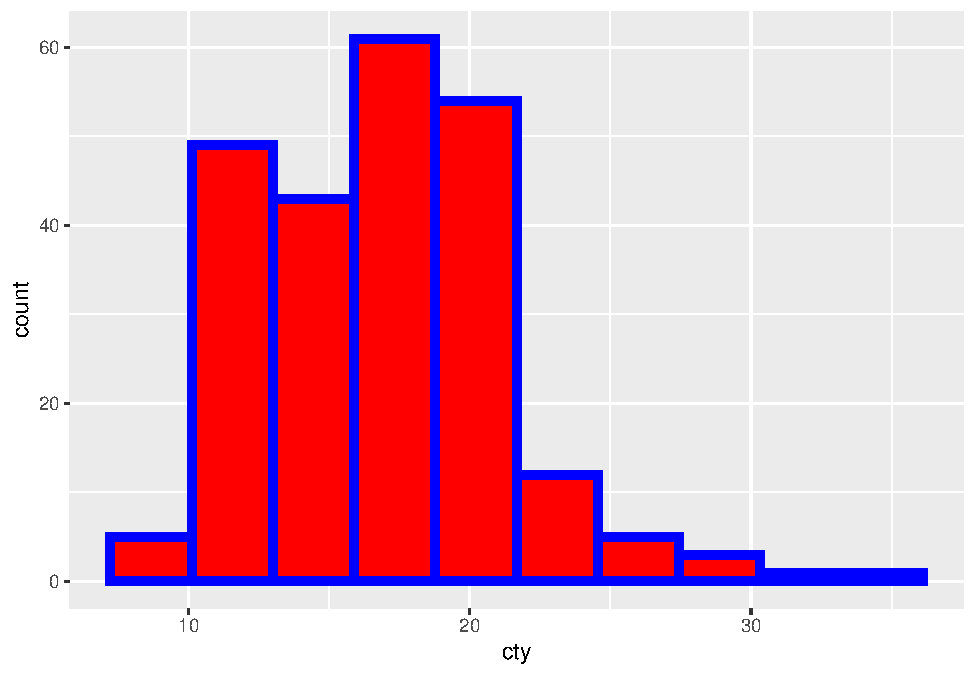
\includegraphics{02_ggplot2_files/figure-latex/unnamed-chunk-5-3.pdf}

\begin{Shaded}
\begin{Highlighting}[]
\NormalTok{v4}\OtherTok{\textless{}{-}} \FunctionTok{ggplot}\NormalTok{(dados, }\FunctionTok{aes}\NormalTok{(}\AttributeTok{x =}\NormalTok{ cty)) }\SpecialCharTok{+} 
  \FunctionTok{geom\_histogram}\NormalTok{(}\FunctionTok{aes}\NormalTok{(}\AttributeTok{y =} \FunctionTok{after\_stat}\NormalTok{(density)),}
                 \AttributeTok{bins =} \DecValTok{10}\NormalTok{, }\AttributeTok{fill =} \StringTok{"yellow"}\NormalTok{, }\AttributeTok{col =} \StringTok{"red"}\NormalTok{) }\SpecialCharTok{+}
  \FunctionTok{geom\_density}\NormalTok{(}\AttributeTok{col =} \StringTok{"blue"}\NormalTok{, }\AttributeTok{lwd =}\DecValTok{3}\NormalTok{)}
\NormalTok{v4}
\end{Highlighting}
\end{Shaded}

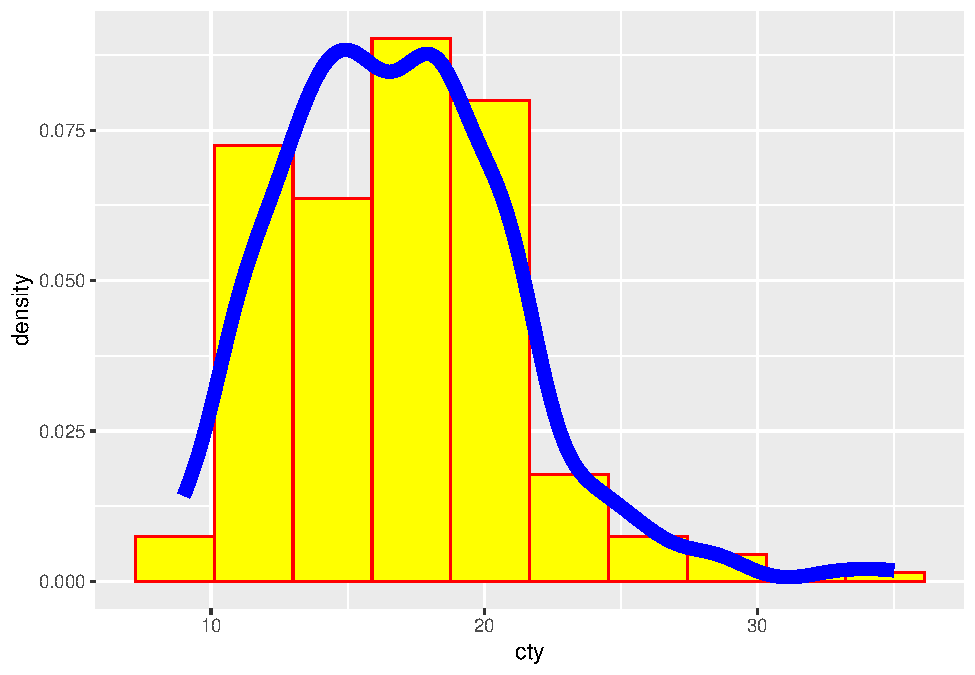
\includegraphics{02_ggplot2_files/figure-latex/unnamed-chunk-5-4.pdf}

\begin{Shaded}
\begin{Highlighting}[]
\CommentTok{\# Adicional (estatístic experimental)}
\FunctionTok{ggplot}\NormalTok{(dados, }\FunctionTok{aes}\NormalTok{(}\AttributeTok{x =}\NormalTok{ drv, }\AttributeTok{y =}\NormalTok{ cty, }\AttributeTok{col =}\NormalTok{ drv)) }\SpecialCharTok{+} 
  \FunctionTok{geom\_boxplot}\NormalTok{()}\SpecialCharTok{+}
  \FunctionTok{theme\_bw}\NormalTok{()}\SpecialCharTok{+}
  \FunctionTok{theme}\NormalTok{(}\AttributeTok{legend.position =} \StringTok{"none"}\NormalTok{)}
\end{Highlighting}
\end{Shaded}

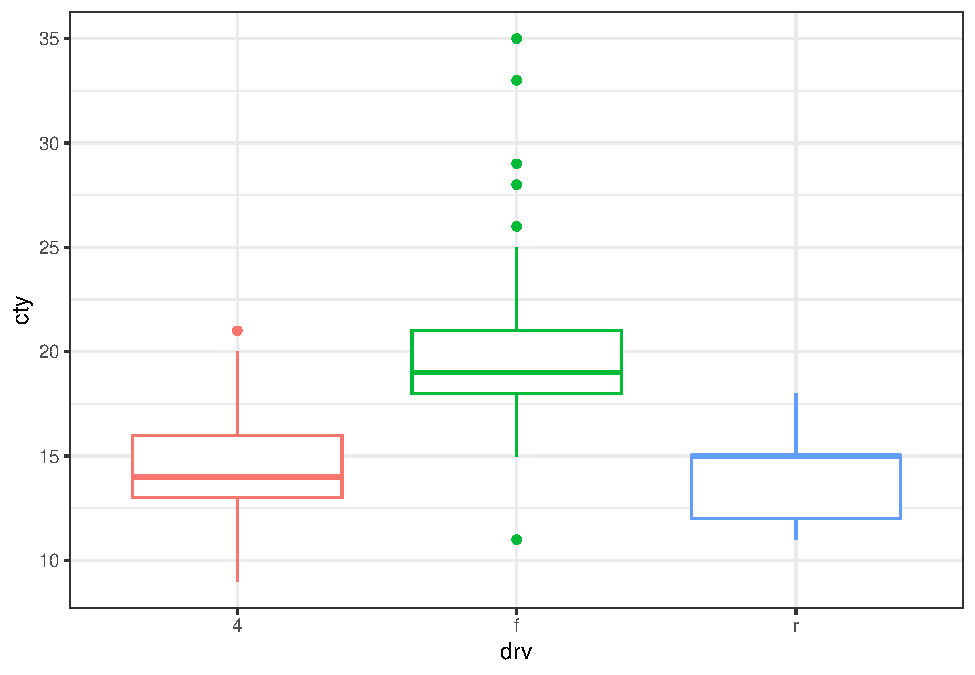
\includegraphics{02_ggplot2_files/figure-latex/unnamed-chunk-5-5.pdf}

\hypertarget{gridextra-e-patchwork}{%
\section{gridExtra e patchwork}\label{gridextra-e-patchwork}}

Alguns links

\href{https://patchwork.data-imaginist.com/articles/guides/assembly.html}{link 1: patchwork}

\href{https://patchwork.data-imaginist.com/articles/patchwork.html}{link 2: patchwork}

\begin{Shaded}
\begin{Highlighting}[]
\CommentTok{\# gridExtra}
\FunctionTok{grid.arrange}\NormalTok{(v1, v2, v3, v4) }
\end{Highlighting}
\end{Shaded}

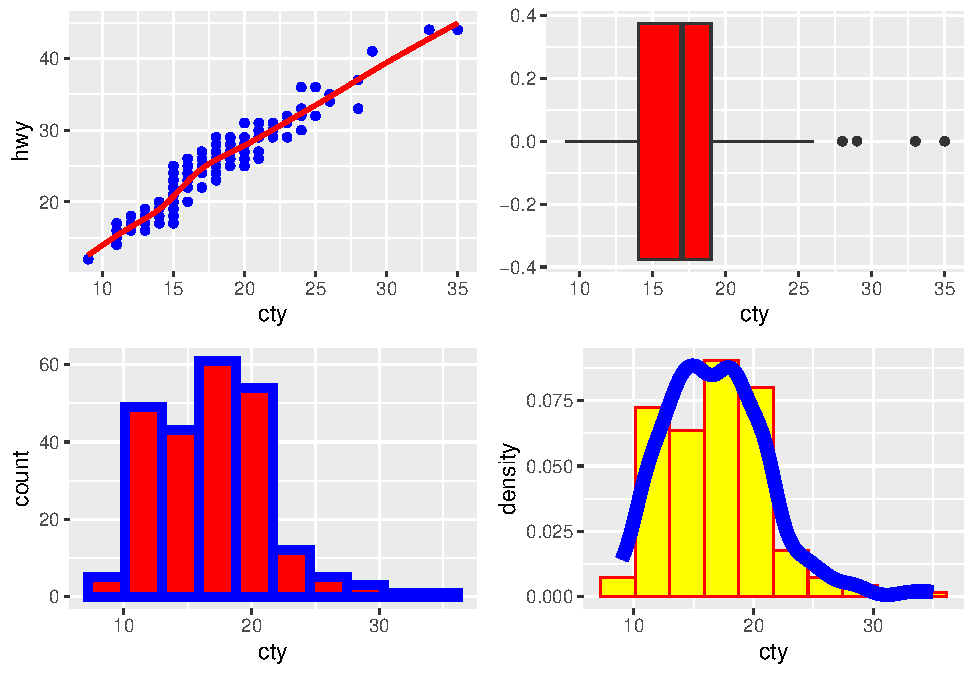
\includegraphics{02_ggplot2_files/figure-latex/unnamed-chunk-6-1.pdf}

\begin{Shaded}
\begin{Highlighting}[]
\CommentTok{\# patchwork}
\NormalTok{v1 }\SpecialCharTok{+}\NormalTok{ v2}
\end{Highlighting}
\end{Shaded}

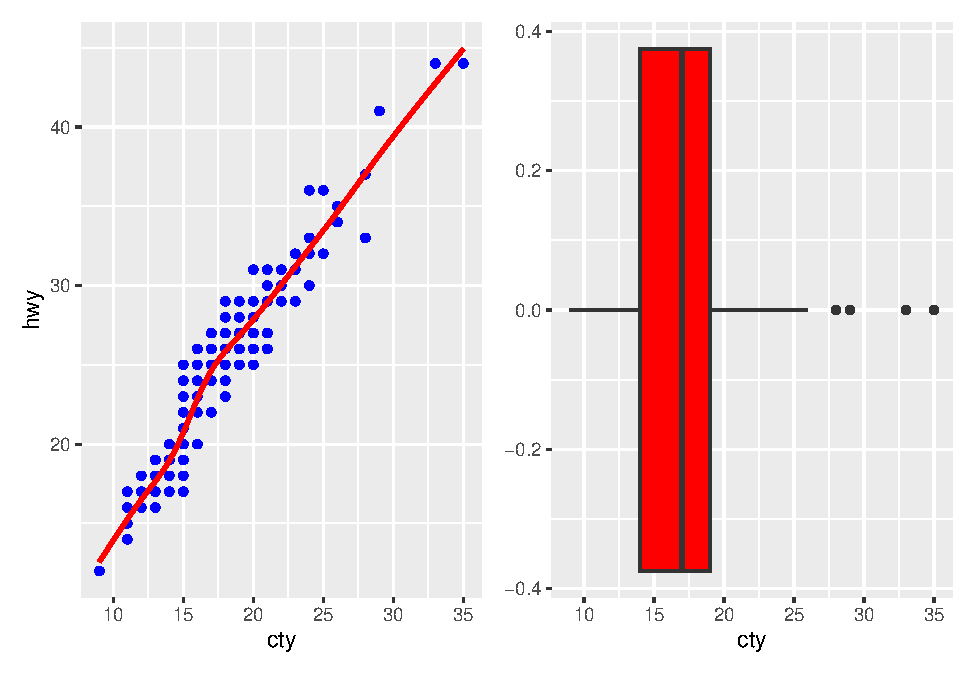
\includegraphics{02_ggplot2_files/figure-latex/unnamed-chunk-6-2.pdf}

\begin{Shaded}
\begin{Highlighting}[]
\NormalTok{v1 }\SpecialCharTok{|}\NormalTok{ v2}
\end{Highlighting}
\end{Shaded}

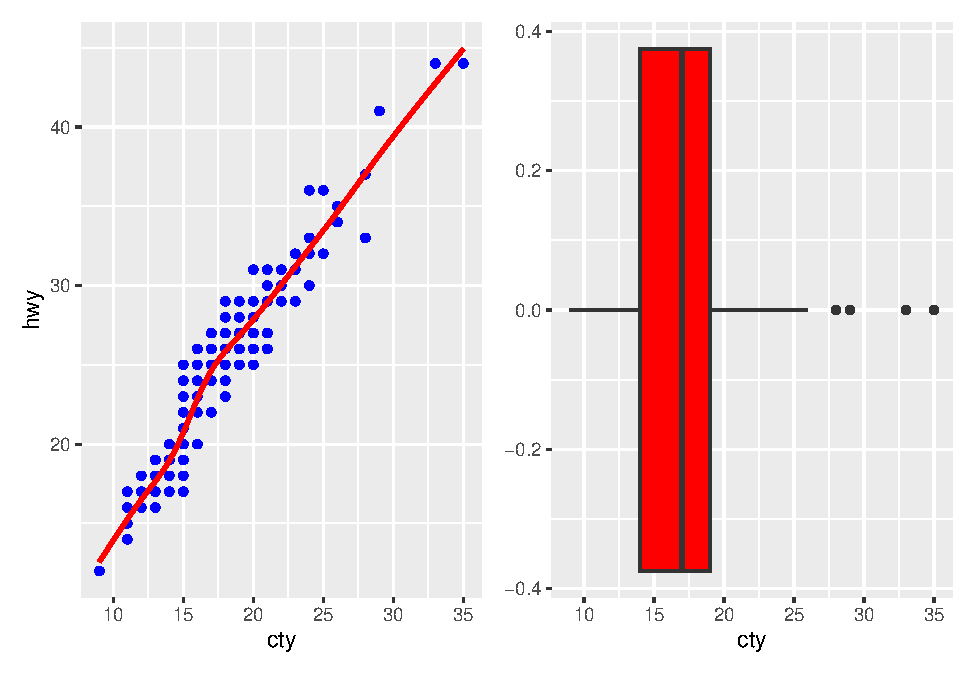
\includegraphics{02_ggplot2_files/figure-latex/unnamed-chunk-6-3.pdf}

\begin{Shaded}
\begin{Highlighting}[]
\NormalTok{v1 }\SpecialCharTok{/}\NormalTok{ v2}
\end{Highlighting}
\end{Shaded}

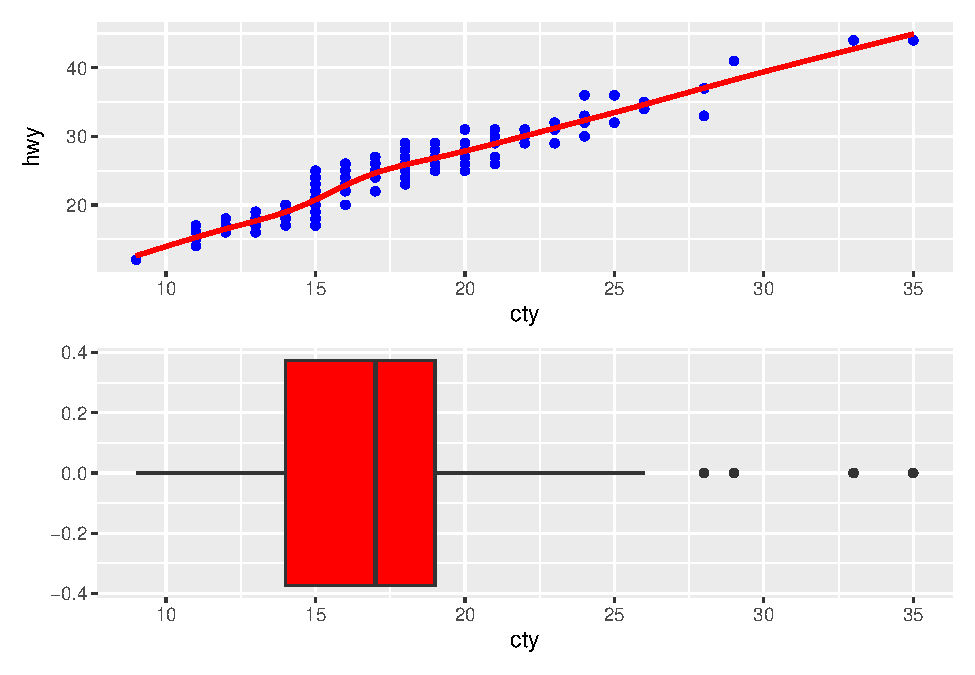
\includegraphics{02_ggplot2_files/figure-latex/unnamed-chunk-6-4.pdf}

\begin{Shaded}
\begin{Highlighting}[]
\NormalTok{v1 }\SpecialCharTok{+}\NormalTok{ v2 }\SpecialCharTok{+}\NormalTok{ v3}
\end{Highlighting}
\end{Shaded}

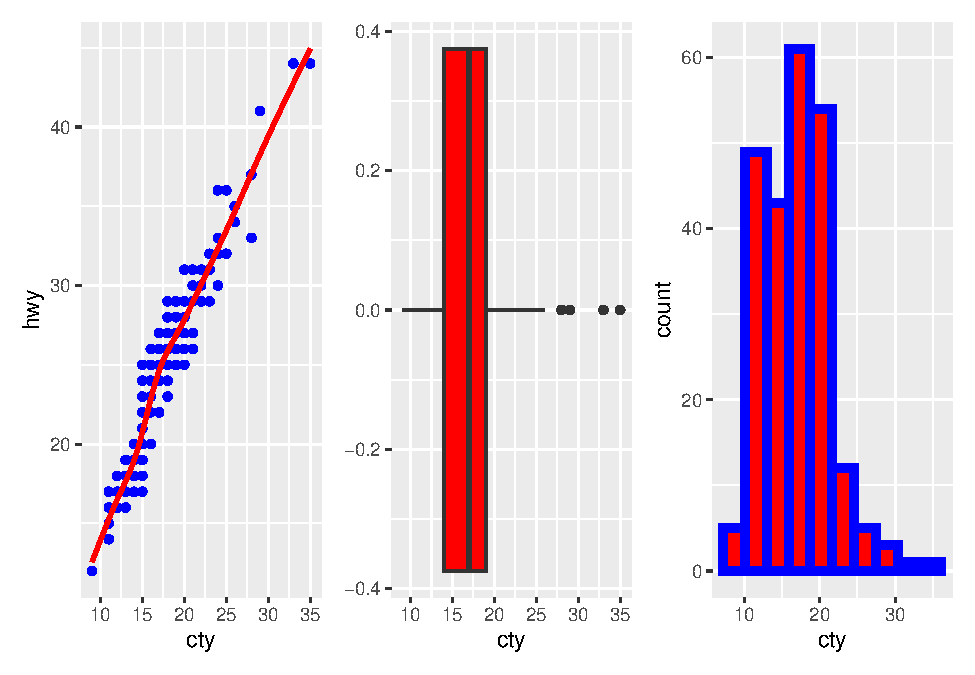
\includegraphics{02_ggplot2_files/figure-latex/unnamed-chunk-6-5.pdf}

\begin{Shaded}
\begin{Highlighting}[]
\NormalTok{v1 }\SpecialCharTok{+}\NormalTok{ (v2 }\SpecialCharTok{+}\NormalTok{ v3)}
\end{Highlighting}
\end{Shaded}

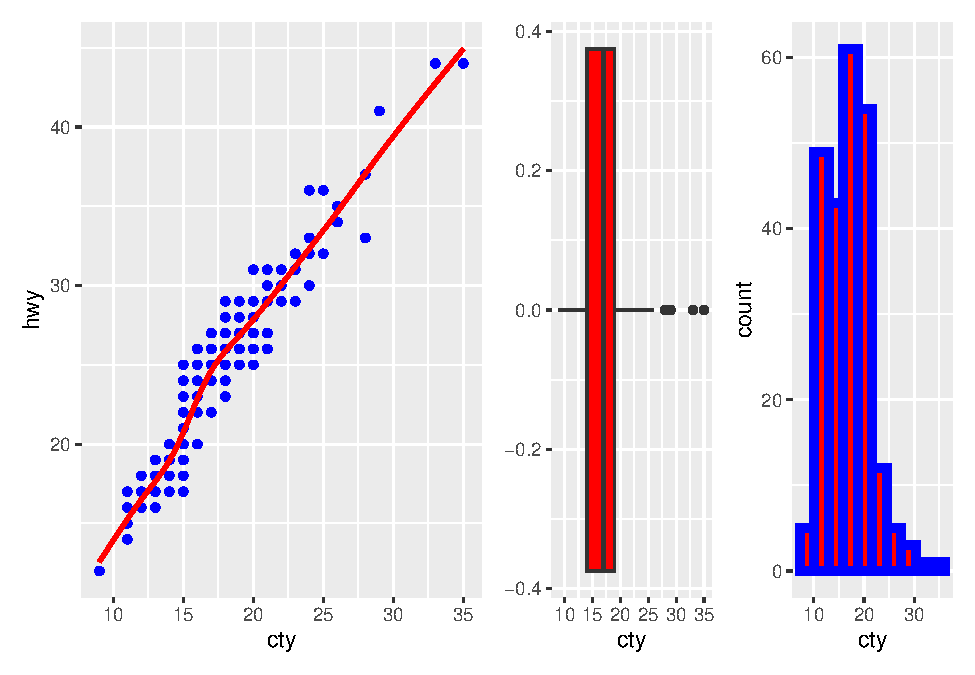
\includegraphics{02_ggplot2_files/figure-latex/unnamed-chunk-6-6.pdf}

\begin{Shaded}
\begin{Highlighting}[]
\NormalTok{v1 }\SpecialCharTok{|}\NormalTok{ (v2 }\SpecialCharTok{/}\NormalTok{ v3)}
\end{Highlighting}
\end{Shaded}

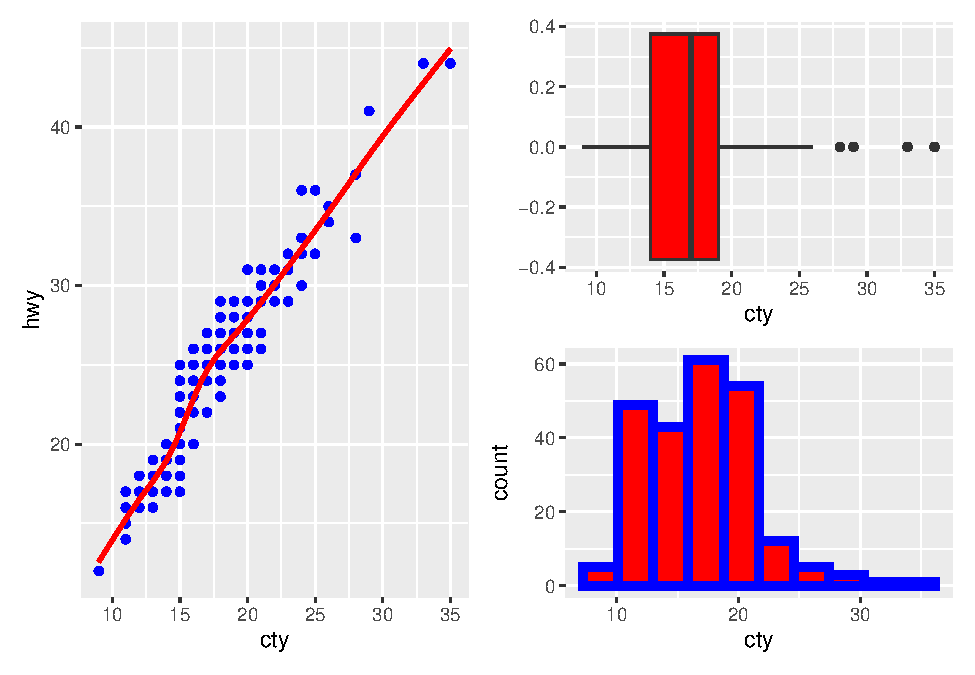
\includegraphics{02_ggplot2_files/figure-latex/unnamed-chunk-6-7.pdf}

\begin{Shaded}
\begin{Highlighting}[]
\NormalTok{v1 }\SpecialCharTok{/}\NormalTok{ (v2 }\SpecialCharTok{+}\NormalTok{ v3)}
\end{Highlighting}
\end{Shaded}

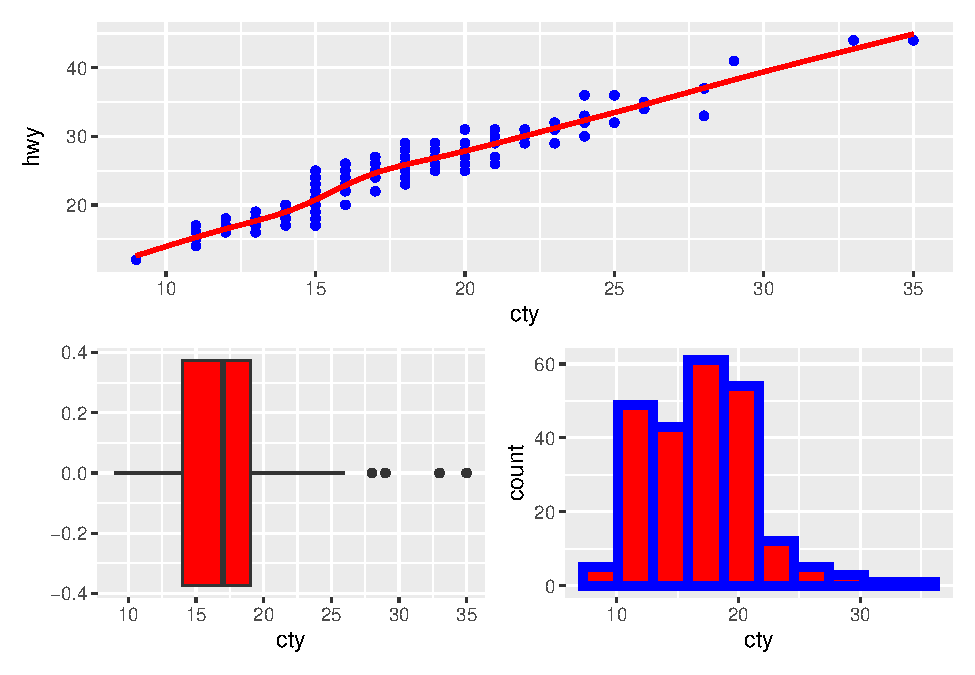
\includegraphics{02_ggplot2_files/figure-latex/unnamed-chunk-6-8.pdf}

\begin{Shaded}
\begin{Highlighting}[]
\NormalTok{v1 }\SpecialCharTok{+}\NormalTok{ v2 }\SpecialCharTok{+}\NormalTok{ v3 }\SpecialCharTok{+}\NormalTok{ v4 }
\end{Highlighting}
\end{Shaded}

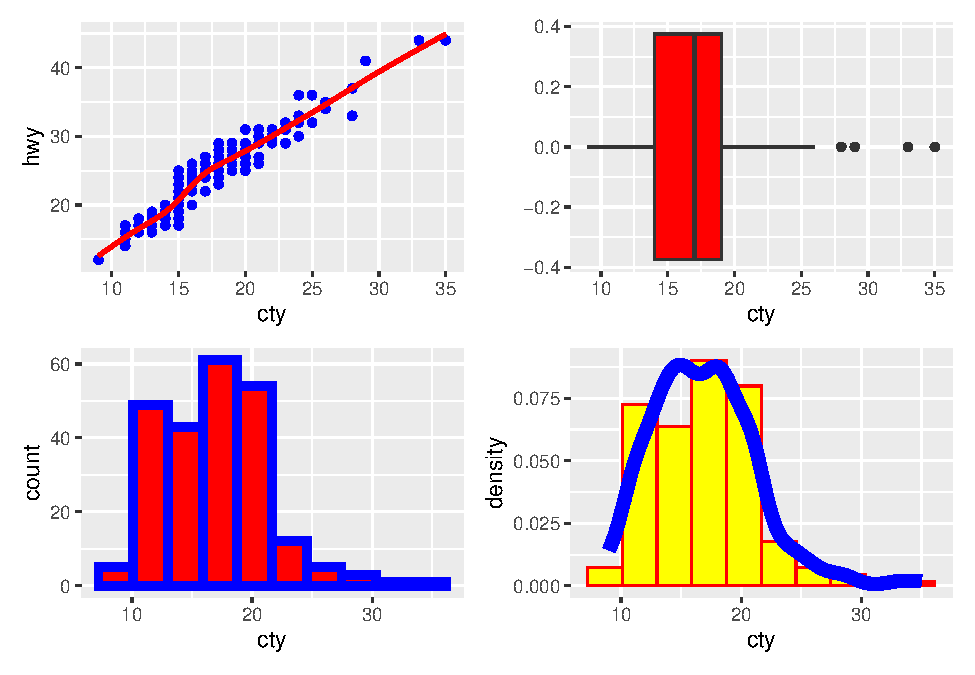
\includegraphics{02_ggplot2_files/figure-latex/unnamed-chunk-6-9.pdf}

\begin{Shaded}
\begin{Highlighting}[]
\NormalTok{v1}\SpecialCharTok{/}\NormalTok{(v2}\SpecialCharTok{+}\NormalTok{v3}\SpecialCharTok{+}\NormalTok{v4)}
\end{Highlighting}
\end{Shaded}

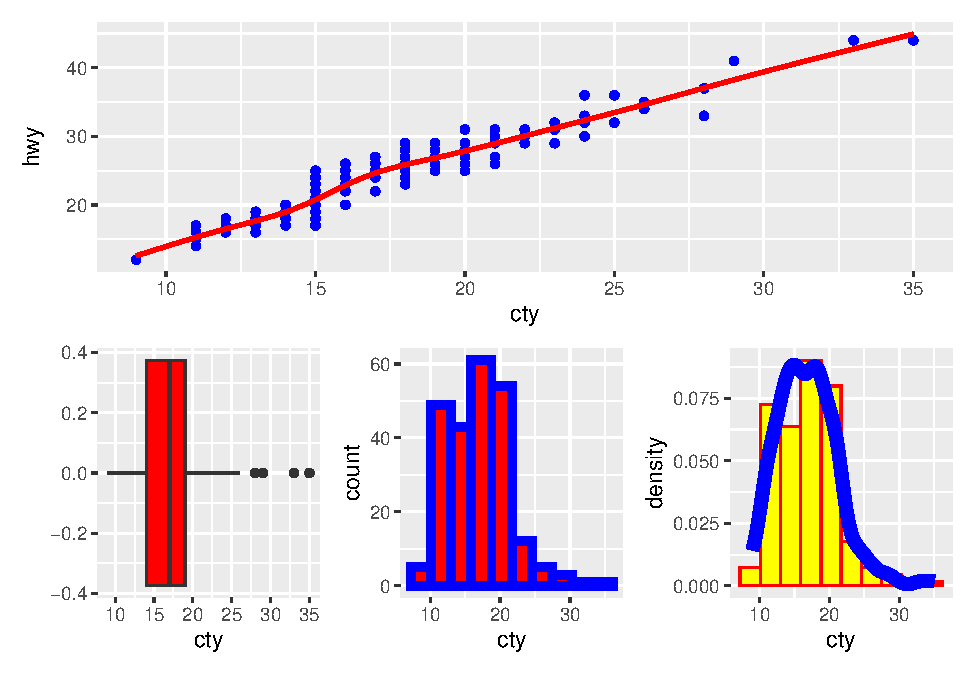
\includegraphics{02_ggplot2_files/figure-latex/unnamed-chunk-6-10.pdf}

\begin{Shaded}
\begin{Highlighting}[]
\NormalTok{v1  }\SpecialCharTok{+}\NormalTok{ (v2 }\SpecialCharTok{+}\NormalTok{ v3 }\SpecialCharTok{+}\NormalTok{ v4)}
\end{Highlighting}
\end{Shaded}

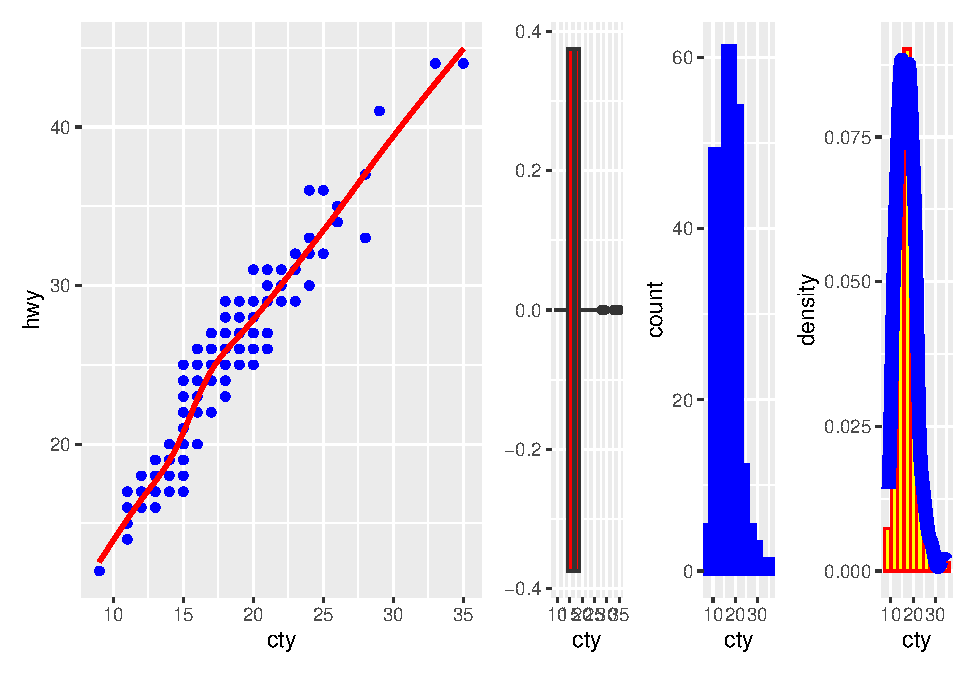
\includegraphics{02_ggplot2_files/figure-latex/unnamed-chunk-6-11.pdf}

\begin{Shaded}
\begin{Highlighting}[]
\NormalTok{v1  }\SpecialCharTok{+}\NormalTok{ v2 }\SpecialCharTok{+}\NormalTok{ (v3 }\SpecialCharTok{+}\NormalTok{ v4)}
\end{Highlighting}
\end{Shaded}

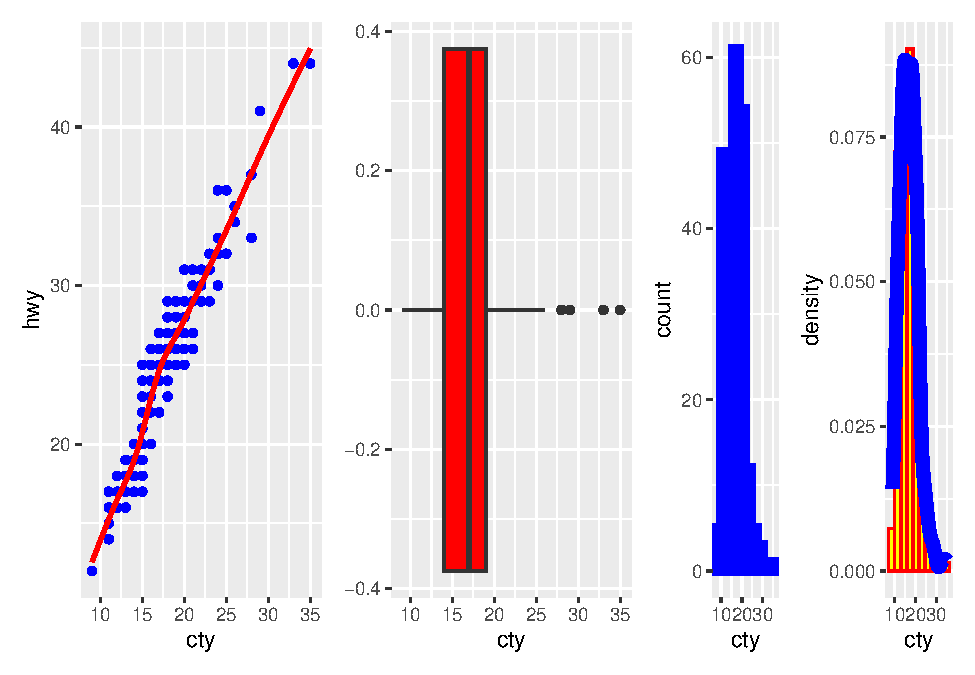
\includegraphics{02_ggplot2_files/figure-latex/unnamed-chunk-6-12.pdf}

\begin{Shaded}
\begin{Highlighting}[]
\NormalTok{(v1 }\SpecialCharTok{|}\NormalTok{ v2 }\SpecialCharTok{|}\NormalTok{ v3) }\SpecialCharTok{/}\NormalTok{ v4}
\end{Highlighting}
\end{Shaded}

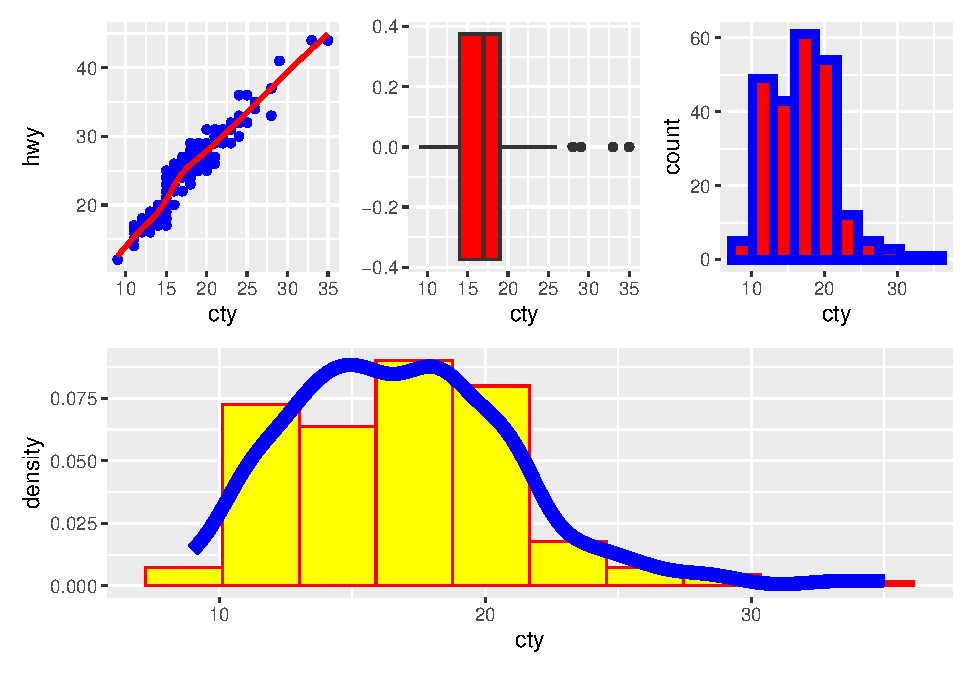
\includegraphics{02_ggplot2_files/figure-latex/unnamed-chunk-6-13.pdf}

\hypertarget{bar-col-density-density2d}{%
\section{bar, col, density, density2d}\label{bar-col-density-density2d}}

\begin{Shaded}
\begin{Highlighting}[]
\NormalTok{v5 }\OtherTok{\textless{}{-}} \FunctionTok{ggplot}\NormalTok{(dados , }\FunctionTok{aes}\NormalTok{(}\AttributeTok{x =}\NormalTok{ manufacturer)) }\SpecialCharTok{+} 
  \FunctionTok{geom\_bar}\NormalTok{()}\SpecialCharTok{+} 
  \FunctionTok{theme}\NormalTok{(}\AttributeTok{axis.text.x =} \FunctionTok{element\_text}\NormalTok{(}\AttributeTok{angle =} \DecValTok{45}\NormalTok{))}
\NormalTok{v5}
\end{Highlighting}
\end{Shaded}

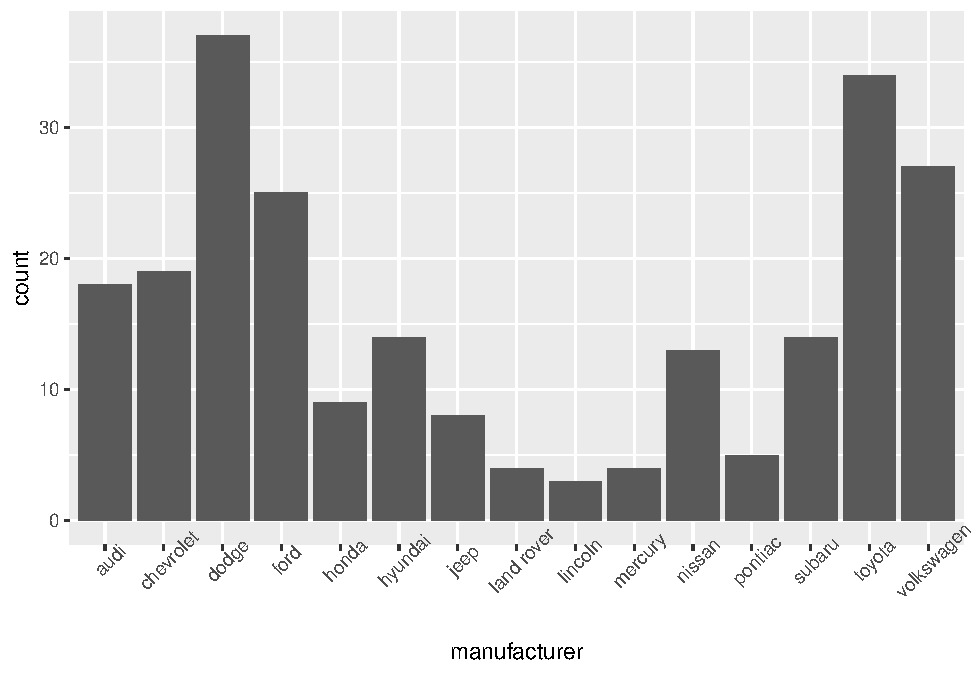
\includegraphics{02_ggplot2_files/figure-latex/unnamed-chunk-7-1.pdf}

\begin{Shaded}
\begin{Highlighting}[]
\CommentTok{\# Dúvidas no geom\_col}
\NormalTok{v6 }\OtherTok{\textless{}{-}} \FunctionTok{ggplot}\NormalTok{(dados , }\FunctionTok{aes}\NormalTok{(}\AttributeTok{x =}\NormalTok{ manufacturer, }\AttributeTok{y =}\NormalTok{ cty)) }\SpecialCharTok{+} 
  \FunctionTok{geom\_col}\NormalTok{()}\SpecialCharTok{+}
  \FunctionTok{theme}\NormalTok{(}\AttributeTok{axis.text.x =} \FunctionTok{element\_text}\NormalTok{(}\AttributeTok{angle =} \DecValTok{45}\NormalTok{))}
\NormalTok{v6}
\end{Highlighting}
\end{Shaded}

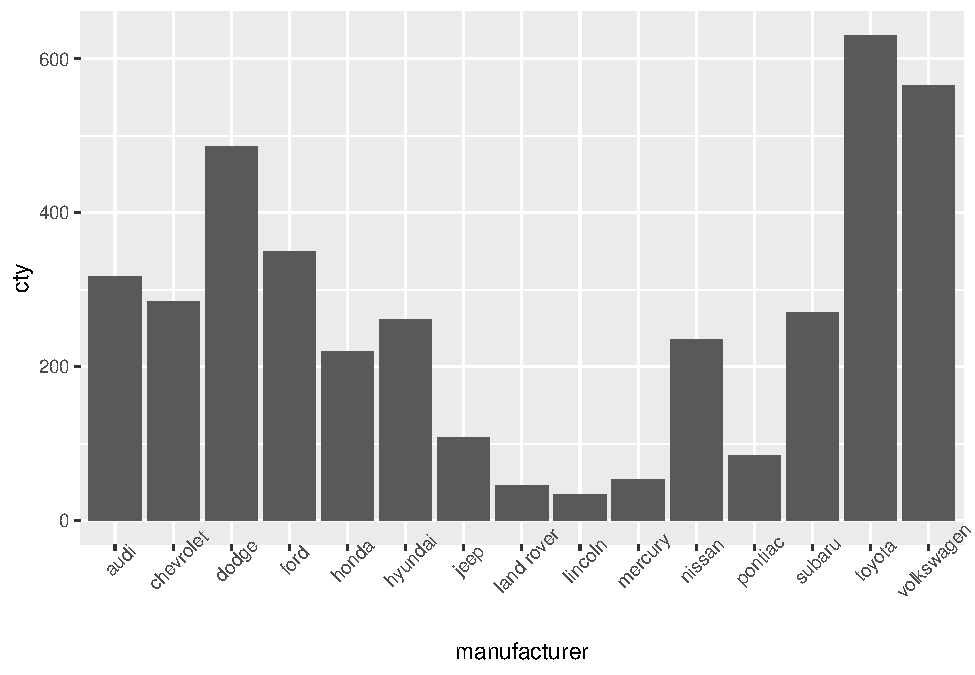
\includegraphics{02_ggplot2_files/figure-latex/unnamed-chunk-7-2.pdf}

\begin{Shaded}
\begin{Highlighting}[]
\NormalTok{dados }\SpecialCharTok{\%\textgreater{}\%} 
  \FunctionTok{select}\NormalTok{(manufacturer, cty) }\SpecialCharTok{\%\textgreater{}\%} 
  \FunctionTok{group\_by}\NormalTok{(manufacturer) }\SpecialCharTok{\%\textgreater{}\%} 
  \FunctionTok{summarise}\NormalTok{(}\AttributeTok{soma\_total\_cty =} \FunctionTok{sum}\NormalTok{(cty),}
            \AttributeTok{n =} \FunctionTok{n}\NormalTok{())}
\end{Highlighting}
\end{Shaded}

\begin{verbatim}
## # A tibble: 15 x 3
##    manufacturer soma_total_cty     n
##    <chr>                 <int> <int>
##  1 audi                    317    18
##  2 chevrolet               285    19
##  3 dodge                   486    37
##  4 ford                    350    25
##  5 honda                   220     9
##  6 hyundai                 261    14
##  7 jeep                    108     8
##  8 land rover               46     4
##  9 lincoln                  34     3
## 10 mercury                  53     4
## 11 nissan                  235    13
## 12 pontiac                  85     5
## 13 subaru                  270    14
## 14 toyota                  630    34
## 15 volkswagen              565    27
\end{verbatim}

\begin{Shaded}
\begin{Highlighting}[]
\CommentTok{\# dados \%\textgreater{}\% }
\CommentTok{\#   filter(manufacturer == "audi") \%\textgreater{}\% }
\CommentTok{\#   select(cty) \%\textgreater{}\% }
\CommentTok{\#   sum()}
\NormalTok{v7 }\OtherTok{\textless{}{-}} \FunctionTok{ggplot}\NormalTok{(dados , }\FunctionTok{aes}\NormalTok{(}\AttributeTok{x =}\NormalTok{ cty)) }\SpecialCharTok{+} 
  \FunctionTok{geom\_density}\NormalTok{()}
\NormalTok{v7}
\end{Highlighting}
\end{Shaded}

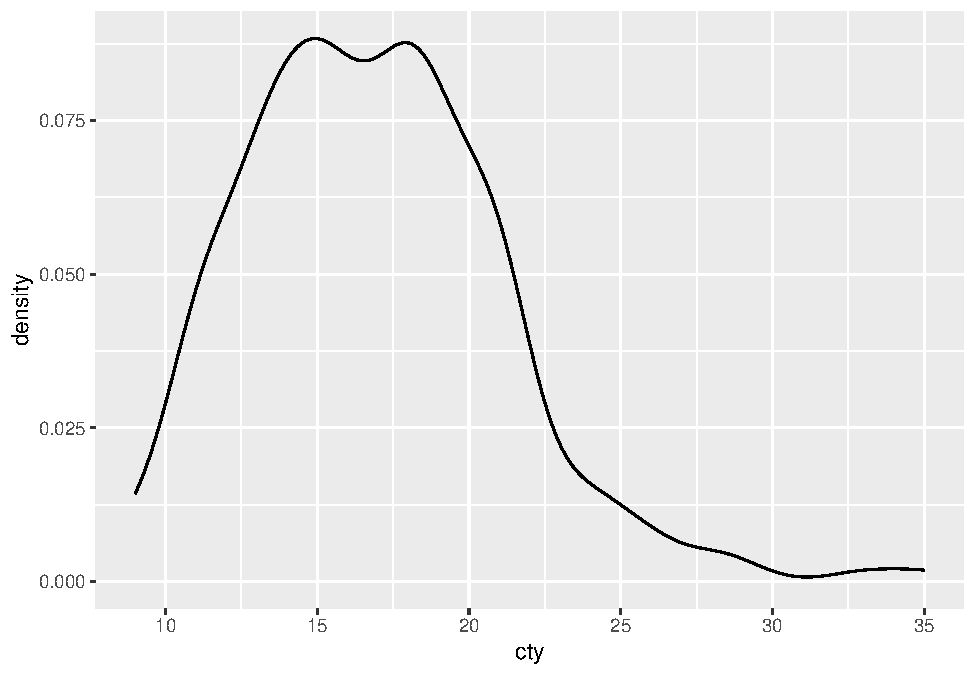
\includegraphics{02_ggplot2_files/figure-latex/unnamed-chunk-7-3.pdf}

\begin{Shaded}
\begin{Highlighting}[]
\NormalTok{v8 }\OtherTok{\textless{}{-}} \FunctionTok{ggplot}\NormalTok{(dados, }\FunctionTok{aes}\NormalTok{(}\AttributeTok{x =}\NormalTok{ cty, }\AttributeTok{y =}\NormalTok{ hwy)) }\SpecialCharTok{+} 
  \FunctionTok{geom\_density2d}\NormalTok{()}\SpecialCharTok{+}
  \FunctionTok{geom\_point}\NormalTok{(}\AttributeTok{colour =} \StringTok{"red"}\NormalTok{)}
\NormalTok{v8}
\end{Highlighting}
\end{Shaded}

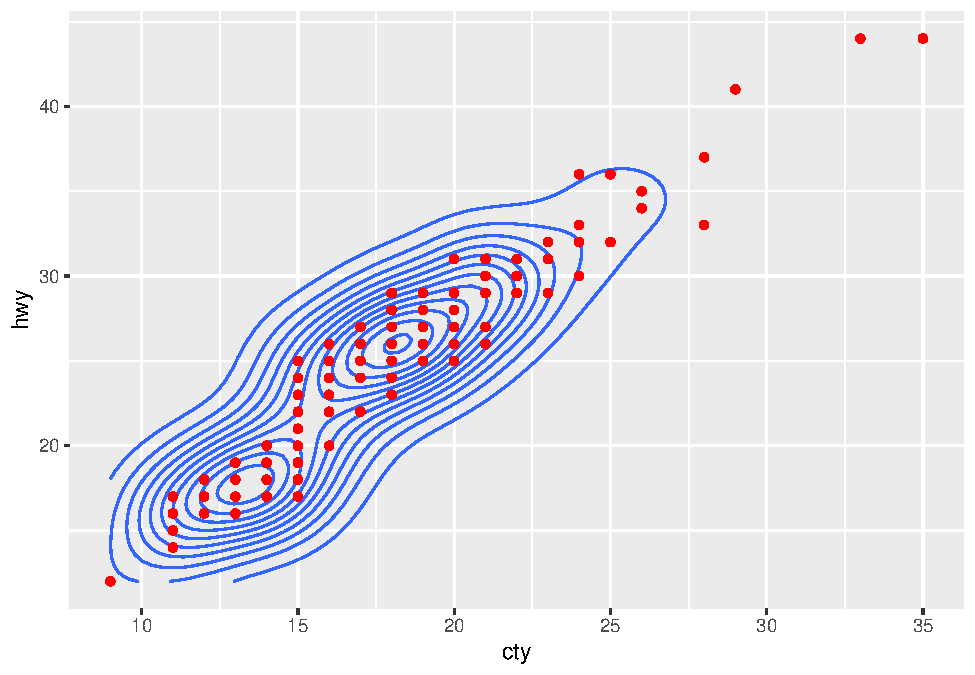
\includegraphics{02_ggplot2_files/figure-latex/unnamed-chunk-7-4.pdf}

\begin{Shaded}
\begin{Highlighting}[]
\NormalTok{(v5}\SpecialCharTok{+}\NormalTok{v6)}\SpecialCharTok{/}\NormalTok{ (v7 }\SpecialCharTok{+}\NormalTok{ v8)}
\end{Highlighting}
\end{Shaded}

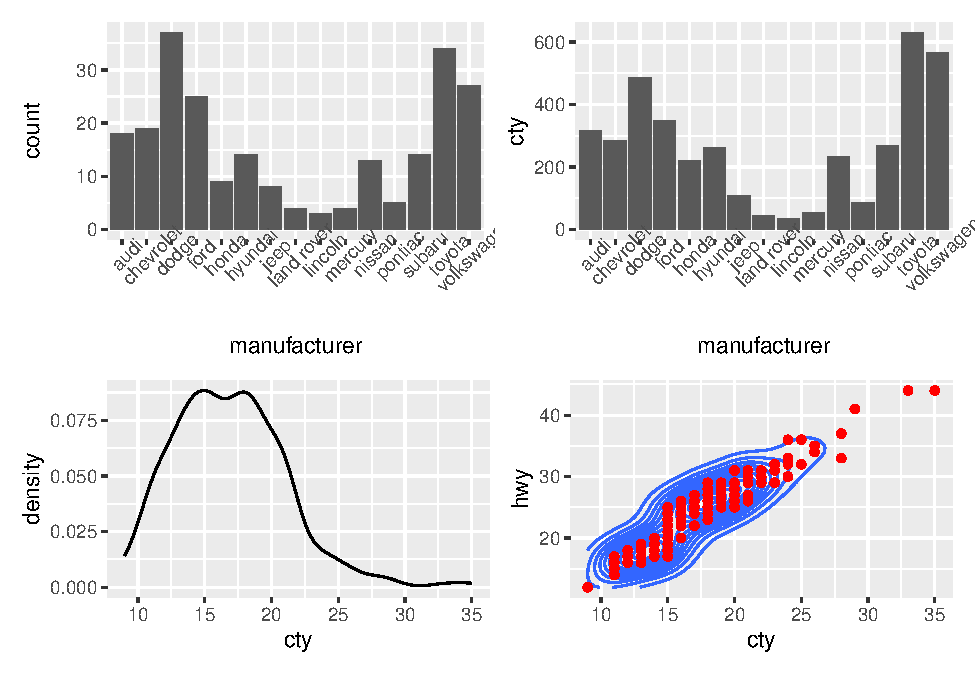
\includegraphics{02_ggplot2_files/figure-latex/unnamed-chunk-7-5.pdf}

\begin{Shaded}
\begin{Highlighting}[]
\CommentTok{\# Deixar pra depois...}
\NormalTok{ dados }\SpecialCharTok{\%\textgreater{}\%} 
    \FunctionTok{select}\NormalTok{(manufacturer, hwy, year) }\SpecialCharTok{\%\textgreater{}\%} 
    \FunctionTok{filter}\NormalTok{(manufacturer }\SpecialCharTok{==} \StringTok{"audi"}\NormalTok{, year }\SpecialCharTok{==} \StringTok{"1999"}\NormalTok{) }\SpecialCharTok{\%\textgreater{}\%} 
    \FunctionTok{summarise}\NormalTok{(}\AttributeTok{media =} \FunctionTok{max}\NormalTok{(hwy))}
\end{Highlighting}
\end{Shaded}

\begin{verbatim}
## # A tibble: 1 x 1
##   media
##   <int>
## 1    29
\end{verbatim}

\begin{Shaded}
\begin{Highlighting}[]
\CommentTok{\# plotly}
\FunctionTok{ggplotly}\NormalTok{(}
\FunctionTok{ggplot}\NormalTok{(dados, }\FunctionTok{aes}\NormalTok{(}\AttributeTok{x =}\NormalTok{ manufacturer, }\AttributeTok{y =}\NormalTok{ hwy, }\AttributeTok{fill =} \FunctionTok{factor}\NormalTok{(year))) }\SpecialCharTok{+} 
  \FunctionTok{geom\_col}\NormalTok{(}\AttributeTok{position =} \StringTok{"dodge"}\NormalTok{) }\SpecialCharTok{+} 
  \FunctionTok{labs}\NormalTok{(}\AttributeTok{fill =} \StringTok{"year"}\NormalTok{) }\SpecialCharTok{+}
  \FunctionTok{theme}\NormalTok{(}\AttributeTok{axis.text.x =} \FunctionTok{element\_text}\NormalTok{(}\AttributeTok{angle =} \DecValTok{45}\NormalTok{)))}

\NormalTok{dados }\SpecialCharTok{\%\textgreater{}\%} \FunctionTok{select}\NormalTok{(manufacturer, hwy, year) }\SpecialCharTok{\%\textgreater{}\%} 
  \FunctionTok{group\_by}\NormalTok{(manufacturer, year) }\SpecialCharTok{\%\textgreater{}\%} 
  \FunctionTok{summarise}\NormalTok{(}\AttributeTok{media =} \FunctionTok{mean}\NormalTok{(hwy))}
\end{Highlighting}
\end{Shaded}

\begin{Shaded}
\begin{Highlighting}[]
\CommentTok{\# Para pensar}

\NormalTok{(dados\_trat }\OtherTok{\textless{}{-}} \FunctionTok{data.frame}\NormalTok{(}\AttributeTok{tratamento =}\NormalTok{ LETTERS[}\DecValTok{1}\SpecialCharTok{:}\DecValTok{3}\NormalTok{], }
                         \AttributeTok{resposta =} \FunctionTok{c}\NormalTok{(}\FloatTok{2.3}\NormalTok{, }\FloatTok{1.9}\NormalTok{, }\FloatTok{3.2}\NormalTok{)))}
\end{Highlighting}
\end{Shaded}

\begin{verbatim}
##   tratamento resposta
## 1          A      2.3
## 2          B      1.9
## 3          C      3.2
\end{verbatim}

\begin{Shaded}
\begin{Highlighting}[]
\FunctionTok{ggplot}\NormalTok{(dados\_trat, }\FunctionTok{aes}\NormalTok{(tratamento, resposta)) }\SpecialCharTok{+}
  \FunctionTok{geom\_col}\NormalTok{(}\AttributeTok{fill =} \StringTok{"red"}\NormalTok{)}
\end{Highlighting}
\end{Shaded}

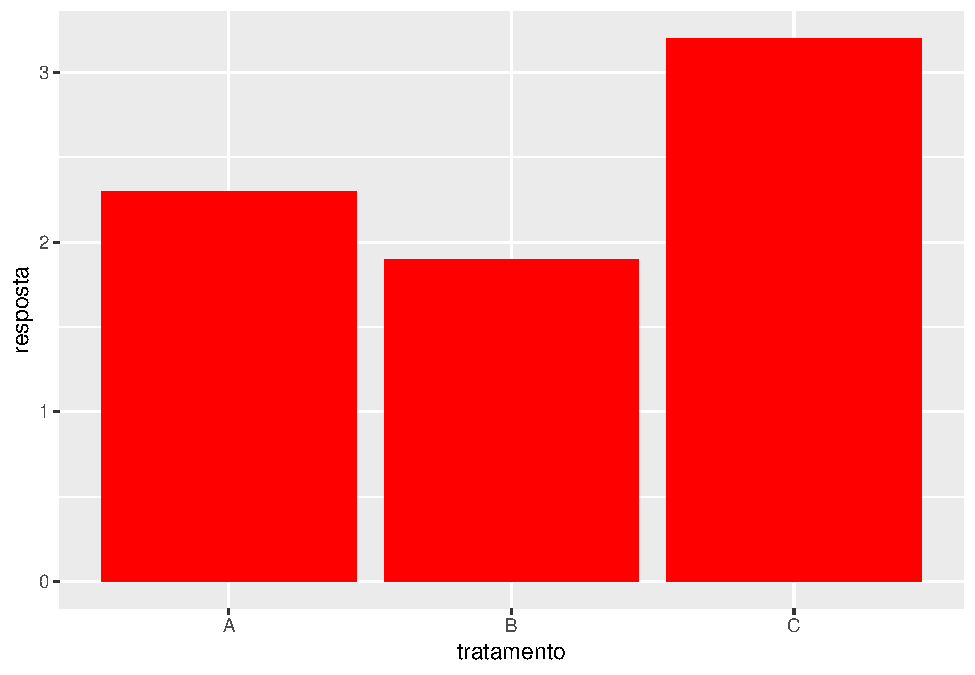
\includegraphics{02_ggplot2_files/figure-latex/unnamed-chunk-9-1.pdf}

\begin{Shaded}
\begin{Highlighting}[]
\CommentTok{\# Mais detalhes...}
\NormalTok{dados }\SpecialCharTok{\%\textgreater{}\%} \FunctionTok{select}\NormalTok{(manufacturer, hwy, year) }\SpecialCharTok{\%\textgreater{}\%} 
  \FunctionTok{group\_by}\NormalTok{(manufacturer, year) }\SpecialCharTok{\%\textgreater{}\%} 
  \FunctionTok{summarise}\NormalTok{(}\AttributeTok{media =} \FunctionTok{mean}\NormalTok{(hwy), }\AttributeTok{.groups =} \StringTok{"drop"}\NormalTok{) }\SpecialCharTok{\%\textgreater{}\%} 
  \FunctionTok{ggplot}\NormalTok{(}\FunctionTok{aes}\NormalTok{(}\AttributeTok{x =}\NormalTok{ manufacturer, }\AttributeTok{y =}\NormalTok{ media, }\AttributeTok{fill =} \FunctionTok{factor}\NormalTok{(year)))}\SpecialCharTok{+}
  \FunctionTok{geom\_col}\NormalTok{(}\AttributeTok{position =} \StringTok{"dodge"}\NormalTok{)}\SpecialCharTok{+}
  \FunctionTok{labs}\NormalTok{(}\AttributeTok{fill =} \StringTok{"year"}\NormalTok{) }\SpecialCharTok{+}
  \FunctionTok{theme}\NormalTok{(}\AttributeTok{axis.text.x =} \FunctionTok{element\_text}\NormalTok{(}\AttributeTok{angle =} \DecValTok{45}\NormalTok{))}
\end{Highlighting}
\end{Shaded}

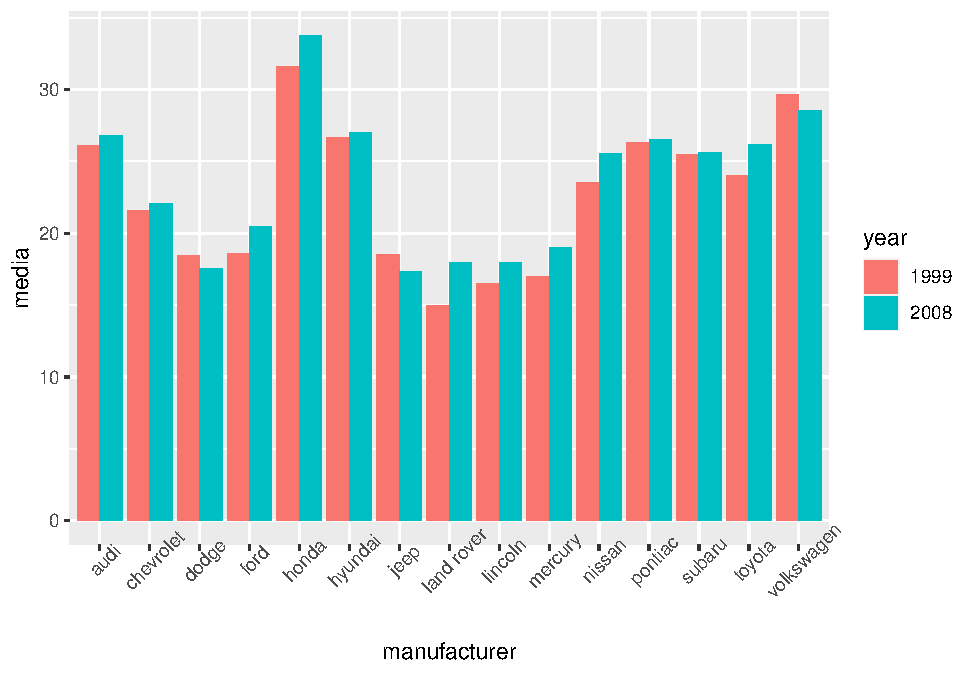
\includegraphics{02_ggplot2_files/figure-latex/unnamed-chunk-9-2.pdf}

\hypertarget{facet_grid-facet_wrap}{%
\section{facet\_grid, facet\_wrap}\label{facet_grid-facet_wrap}}

\begin{Shaded}
\begin{Highlighting}[]
\NormalTok{p1}\OtherTok{\textless{}{-}} \FunctionTok{ggplot}\NormalTok{(dados, }\FunctionTok{aes}\NormalTok{(}\AttributeTok{x =}\NormalTok{ cty, }\AttributeTok{y =}\NormalTok{ hwy)) }\SpecialCharTok{+}
  \FunctionTok{geom\_point}\NormalTok{()}
\NormalTok{p1}
\end{Highlighting}
\end{Shaded}

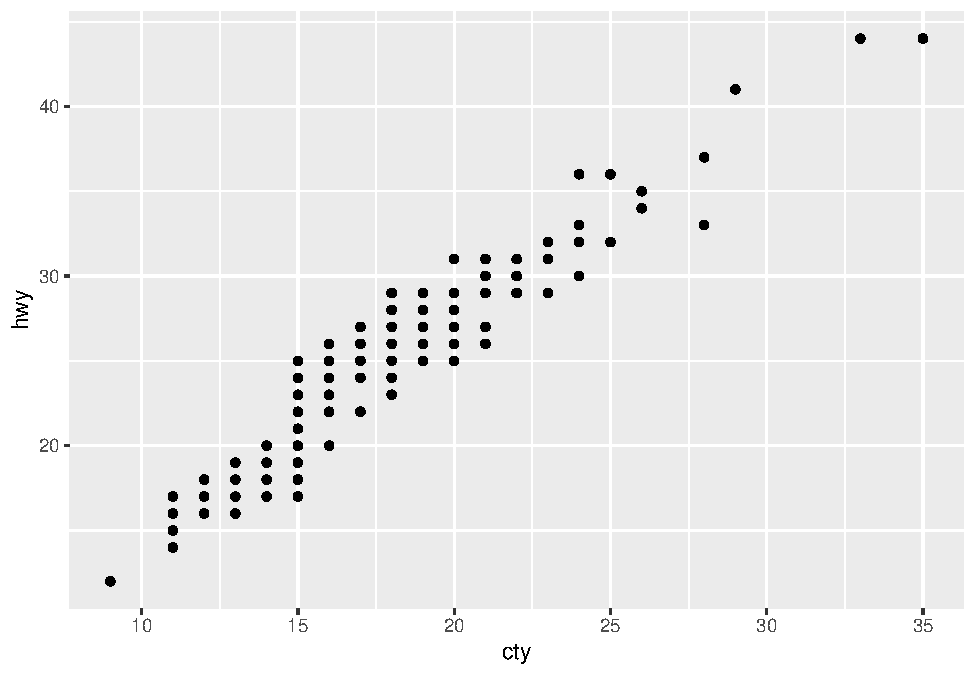
\includegraphics{02_ggplot2_files/figure-latex/unnamed-chunk-10-1.pdf}

\begin{Shaded}
\begin{Highlighting}[]
\NormalTok{p1 }\SpecialCharTok{+} \FunctionTok{facet\_grid}\NormalTok{(}\AttributeTok{rows =} \FunctionTok{vars}\NormalTok{(cyl))}
\end{Highlighting}
\end{Shaded}

\includegraphics{02_ggplot2_files/figure-latex/unnamed-chunk-10-2.pdf}

\begin{Shaded}
\begin{Highlighting}[]
\NormalTok{p1 }\SpecialCharTok{+} \FunctionTok{facet\_grid}\NormalTok{(}\AttributeTok{cols =} \FunctionTok{vars}\NormalTok{(cyl))}
\end{Highlighting}
\end{Shaded}

\includegraphics{02_ggplot2_files/figure-latex/unnamed-chunk-10-3.pdf}

\begin{Shaded}
\begin{Highlighting}[]
\NormalTok{p1 }\SpecialCharTok{+} \FunctionTok{facet\_grid}\NormalTok{(}\SpecialCharTok{\textasciitilde{}}\NormalTok{cyl)}
\end{Highlighting}
\end{Shaded}

\includegraphics{02_ggplot2_files/figure-latex/unnamed-chunk-10-4.pdf}

\begin{Shaded}
\begin{Highlighting}[]
\NormalTok{p1 }\SpecialCharTok{+} \FunctionTok{facet\_grid}\NormalTok{(}\AttributeTok{rows =} \FunctionTok{vars}\NormalTok{(year), }\AttributeTok{cols =}\FunctionTok{vars}\NormalTok{(cyl))}
\end{Highlighting}
\end{Shaded}

\includegraphics{02_ggplot2_files/figure-latex/unnamed-chunk-10-5.pdf}

\begin{Shaded}
\begin{Highlighting}[]
\NormalTok{p1 }\SpecialCharTok{+} \FunctionTok{facet\_grid}\NormalTok{(year}\SpecialCharTok{\textasciitilde{}}\NormalTok{cyl)}
\end{Highlighting}
\end{Shaded}

\includegraphics{02_ggplot2_files/figure-latex/unnamed-chunk-10-6.pdf}

\begin{Shaded}
\begin{Highlighting}[]
\NormalTok{p1 }\SpecialCharTok{+} \FunctionTok{facet\_wrap}\NormalTok{(year }\SpecialCharTok{\textasciitilde{}}\NormalTok{ cyl)}
\end{Highlighting}
\end{Shaded}

\includegraphics{02_ggplot2_files/figure-latex/unnamed-chunk-10-7.pdf}

\begin{Shaded}
\begin{Highlighting}[]
\NormalTok{p1 }\SpecialCharTok{+} \FunctionTok{facet\_wrap}\NormalTok{(cyl }\SpecialCharTok{\textasciitilde{}}\NormalTok{ year)}
\end{Highlighting}
\end{Shaded}

\includegraphics{02_ggplot2_files/figure-latex/unnamed-chunk-10-8.pdf}

\begin{Shaded}
\begin{Highlighting}[]
\NormalTok{p1 }\SpecialCharTok{+} \FunctionTok{facet\_wrap}\NormalTok{(}\SpecialCharTok{\textasciitilde{}}\NormalTok{cyl }\SpecialCharTok{+}\NormalTok{ year)}
\end{Highlighting}
\end{Shaded}

\includegraphics{02_ggplot2_files/figure-latex/unnamed-chunk-10-9.pdf}

\begin{Shaded}
\begin{Highlighting}[]
\NormalTok{p1 }\SpecialCharTok{+} \FunctionTok{facet\_wrap}\NormalTok{(}\SpecialCharTok{\textasciitilde{}}\NormalTok{year }\SpecialCharTok{+}\NormalTok{ cyl)}
\end{Highlighting}
\end{Shaded}

\includegraphics{02_ggplot2_files/figure-latex/unnamed-chunk-10-10.pdf}

\begin{Shaded}
\begin{Highlighting}[]
\NormalTok{p1 }\SpecialCharTok{+} \FunctionTok{facet\_wrap}\NormalTok{(year }\SpecialCharTok{\textasciitilde{}}\NormalTok{ cyl, }\AttributeTok{ncol =} \DecValTok{4}\NormalTok{)}
\end{Highlighting}
\end{Shaded}

\includegraphics{02_ggplot2_files/figure-latex/unnamed-chunk-10-11.pdf}

\begin{Shaded}
\begin{Highlighting}[]
\NormalTok{p1 }\SpecialCharTok{+} \FunctionTok{facet\_wrap}\NormalTok{(cyl }\SpecialCharTok{\textasciitilde{}}\NormalTok{ year, }\AttributeTok{ncol =} \DecValTok{4}\NormalTok{)}
\end{Highlighting}
\end{Shaded}

\includegraphics{02_ggplot2_files/figure-latex/unnamed-chunk-10-12.pdf}

\hypertarget{stat_function}{%
\section{stat\_function}\label{stat_function}}

\begin{Shaded}
\begin{Highlighting}[]
\NormalTok{a}\OtherTok{\textless{}{-}} \SpecialCharTok{{-}}\DecValTok{3} \CommentTok{\# média}
\NormalTok{b}\OtherTok{\textless{}{-}} \DecValTok{4}  \CommentTok{\# desv. padrão}
\FunctionTok{ggplot}\NormalTok{(}\FunctionTok{data.frame}\NormalTok{(}\AttributeTok{x =} \FunctionTok{c}\NormalTok{(a }\SpecialCharTok{{-}} \DecValTok{3}\SpecialCharTok{*}\NormalTok{b, a }\SpecialCharTok{+} \DecValTok{3}\SpecialCharTok{*}\NormalTok{b)), }\FunctionTok{aes}\NormalTok{(x)) }\SpecialCharTok{+} 
  \FunctionTok{stat\_function}\NormalTok{(}\AttributeTok{fun =}\NormalTok{ dnorm, }\AttributeTok{args =} \FunctionTok{list}\NormalTok{(}\AttributeTok{mean =}\NormalTok{ a, }\AttributeTok{sd =}\NormalTok{ b))}\SpecialCharTok{+}
  \FunctionTok{geom\_vline}\NormalTok{(}\AttributeTok{xintercept =} \FunctionTok{c}\NormalTok{(a }\SpecialCharTok{{-}} \DecValTok{3}\SpecialCharTok{*}\NormalTok{b, a, a }\SpecialCharTok{+} \DecValTok{3}\SpecialCharTok{*}\NormalTok{b), }\AttributeTok{col =} \StringTok{"red"}\NormalTok{, }\AttributeTok{lty =} \DecValTok{2}\NormalTok{)}\SpecialCharTok{+}
  \FunctionTok{theme\_minimal}\NormalTok{()}
\end{Highlighting}
\end{Shaded}

\includegraphics{02_ggplot2_files/figure-latex/unnamed-chunk-11-1.pdf}

\hypertarget{stat_summary}{%
\section{stat\_summary}\label{stat_summary}}

\begin{Shaded}
\begin{Highlighting}[]
\FunctionTok{ggplot}\NormalTok{(dados, }\FunctionTok{aes}\NormalTok{(}\AttributeTok{x =}\NormalTok{ manufacturer, }\AttributeTok{y =}\NormalTok{ hwy)) }\SpecialCharTok{+} 
  \FunctionTok{geom\_boxplot}\NormalTok{()}\SpecialCharTok{+}
  \FunctionTok{geom\_point}\NormalTok{(}\AttributeTok{col =} \StringTok{"red"}\NormalTok{, }\AttributeTok{size=}\FloatTok{0.8}\NormalTok{)}\SpecialCharTok{+}
  \FunctionTok{stat\_summary}\NormalTok{(}\AttributeTok{fun =}\NormalTok{ mean, }\AttributeTok{col =} \StringTok{"blue"}\NormalTok{)}\SpecialCharTok{+}
  \FunctionTok{theme\_minimal}\NormalTok{()}\SpecialCharTok{+}
  \FunctionTok{theme}\NormalTok{(}\AttributeTok{axis.text.x =} \FunctionTok{element\_text}\NormalTok{(}\AttributeTok{angle =} \DecValTok{45}\NormalTok{))}
\end{Highlighting}
\end{Shaded}

\includegraphics{02_ggplot2_files/figure-latex/unnamed-chunk-12-1.pdf}

\hypertarget{theme_}{%
\section{theme\_*()}\label{theme_}}

\begin{Shaded}
\begin{Highlighting}[]
\NormalTok{a1}\OtherTok{\textless{}{-}}\NormalTok{ p1 }\SpecialCharTok{+} \FunctionTok{theme\_bw}\NormalTok{() }\SpecialCharTok{+} \FunctionTok{labs}\NormalTok{(}\AttributeTok{title =} \StringTok{"theme\_bw()"}\NormalTok{)}
\NormalTok{a2}\OtherTok{\textless{}{-}}\NormalTok{ p1 }\SpecialCharTok{+} \FunctionTok{theme\_classic}\NormalTok{() }\SpecialCharTok{+} \FunctionTok{labs}\NormalTok{(}\AttributeTok{title =} \StringTok{"theme\_classic()"}\NormalTok{)}
\NormalTok{a3}\OtherTok{\textless{}{-}}\NormalTok{ p1 }\SpecialCharTok{+} \FunctionTok{theme\_light}\NormalTok{() }\SpecialCharTok{+} \FunctionTok{labs}\NormalTok{(}\AttributeTok{title =} \StringTok{"theme\_light()"}\NormalTok{)}
\NormalTok{a4}\OtherTok{\textless{}{-}}\NormalTok{ p1 }\SpecialCharTok{+} \FunctionTok{theme\_minimal}\NormalTok{() }\SpecialCharTok{+} \FunctionTok{labs}\NormalTok{(}\AttributeTok{title =} \StringTok{"theme\_minimal()"}\NormalTok{)}

\NormalTok{a1 }\SpecialCharTok{+}\NormalTok{ a2 }\SpecialCharTok{+}\NormalTok{ a3 }\SpecialCharTok{+}\NormalTok{ a4}
\end{Highlighting}
\end{Shaded}

\includegraphics{02_ggplot2_files/figure-latex/unnamed-chunk-13-1.pdf}

\hypertarget{gruxe1fico-de-perfis-spaguetti-plot}{%
\section{Gráfico de perfis (Spaguetti plot)}\label{gruxe1fico-de-perfis-spaguetti-plot}}

\begin{Shaded}
\begin{Highlighting}[]
\FunctionTok{glimpse}\NormalTok{(Orange)}
\end{Highlighting}
\end{Shaded}

\begin{verbatim}
## Rows: 35
## Columns: 3
## $ Tree          <ord> 1, 1, 1, 1, 1, 1, 1, 2, 2, 2, 2, 2, 2, 2, 3, 3, 3, 3, 3,~
## $ age           <dbl> 118, 484, 664, 1004, 1231, 1372, 1582, 118, 484, 664, 10~
## $ circumference <dbl> 30, 58, 87, 115, 120, 142, 145, 33, 69, 111, 156, 172, 2~
\end{verbatim}

\begin{Shaded}
\begin{Highlighting}[]
\FunctionTok{ggplot}\NormalTok{(Orange, }\FunctionTok{aes}\NormalTok{(}\AttributeTok{x =}\NormalTok{ age, }\AttributeTok{y =}\NormalTok{ circumference, }\AttributeTok{group =}\NormalTok{ Tree, }
                   \AttributeTok{col =}\NormalTok{ Tree)) }\SpecialCharTok{+}
  \FunctionTok{geom\_line}\NormalTok{()}\SpecialCharTok{+}
  \FunctionTok{stat\_summary}\NormalTok{(}\FunctionTok{aes}\NormalTok{(}\AttributeTok{group =} \DecValTok{1}\NormalTok{), }\AttributeTok{fun =}\NormalTok{ mean, }\AttributeTok{col =} \StringTok{"red"}\NormalTok{, }
               \AttributeTok{geom =} \StringTok{"line"}\NormalTok{, }\AttributeTok{size =} \DecValTok{1}\NormalTok{, }\AttributeTok{show.legend =} \ConstantTok{FALSE}\NormalTok{,}
               \AttributeTok{linetype =} \DecValTok{2}\NormalTok{)}\SpecialCharTok{+}
  \FunctionTok{xlim}\NormalTok{(}\DecValTok{0}\NormalTok{, }\DecValTok{1600}\NormalTok{)}\SpecialCharTok{+}
  \FunctionTok{theme\_minimal}\NormalTok{()}
\end{Highlighting}
\end{Shaded}

\includegraphics{02_ggplot2_files/figure-latex/unnamed-chunk-14-1.pdf}

\begin{Shaded}
\begin{Highlighting}[]
\FunctionTok{ggplot}\NormalTok{(Orange, }\FunctionTok{aes}\NormalTok{(}\AttributeTok{x =}\NormalTok{ age, }\AttributeTok{y =}\NormalTok{ circumference, }\AttributeTok{group =}\NormalTok{ Tree)) }\SpecialCharTok{+}
  \FunctionTok{geom\_line}\NormalTok{()}\SpecialCharTok{+}
  \FunctionTok{xlim}\NormalTok{(}\DecValTok{0}\NormalTok{, }\DecValTok{1600}\NormalTok{)}\SpecialCharTok{+}
  \FunctionTok{facet\_wrap}\NormalTok{(}\SpecialCharTok{\textasciitilde{}}\NormalTok{Tree)}\SpecialCharTok{+}
  \FunctionTok{theme\_minimal}\NormalTok{()}\SpecialCharTok{+}
  \FunctionTok{theme}\NormalTok{(}\AttributeTok{legend.position =} \StringTok{"none"}\NormalTok{)}
\end{Highlighting}
\end{Shaded}

\includegraphics{02_ggplot2_files/figure-latex/unnamed-chunk-14-2.pdf}

\hypertarget{plotly}{%
\section{plotly}\label{plotly}}

\href{https://cran.r-project.org/web/packages/plotly/index.html}{plotly cran}

\href{https://plotly-r.com/}{Interactive web-based data visualization with R, plotly, and shiny}

\href{https://plotly.com/r/}{Plotly R Open Source Graphing Library}

\begin{Shaded}
\begin{Highlighting}[]
\FunctionTok{ggplotly}\NormalTok{(v1)}
\FunctionTok{ggplotly}\NormalTok{(v2)}
\FunctionTok{ggplotly}\NormalTok{(v4)}
\FunctionTok{ggplotly}\NormalTok{(v5)}
\end{Highlighting}
\end{Shaded}

\hypertarget{esquisse}{%
\section{esquisse}\label{esquisse}}

Alguns links de interesse

\href{https://cran.r-project.org/web/packages/esquisse/vignettes/get-started.html}{esquisse}

\href{https://cran.r-project.org/web/packages/esquisse/vignettes/shiny-usage.html}{esquisse + shiny}

\begin{Shaded}
\begin{Highlighting}[]
\FunctionTok{esquisser}\NormalTok{(dados)}
\end{Highlighting}
\end{Shaded}

\hypertarget{exemplo-esquisse}{%
\section{Exemplo esquisse}\label{exemplo-esquisse}}

\begin{Shaded}
\begin{Highlighting}[]
\FunctionTok{ggplot}\NormalTok{(dados) }\SpecialCharTok{+}
  \FunctionTok{aes}\NormalTok{(}\AttributeTok{x =}\NormalTok{ displ, }\AttributeTok{y =}\NormalTok{ hwy, }\AttributeTok{colour =}\NormalTok{ drv) }\SpecialCharTok{+}
  \FunctionTok{geom\_point}\NormalTok{(}\AttributeTok{shape =} \StringTok{"circle"}\NormalTok{, }\AttributeTok{size =} \FloatTok{1.85}\NormalTok{) }\SpecialCharTok{+}
  \FunctionTok{scale\_color\_hue}\NormalTok{(}\AttributeTok{direction =} \DecValTok{1}\NormalTok{) }\SpecialCharTok{+}
  \FunctionTok{theme\_minimal}\NormalTok{() }\SpecialCharTok{+}
  \FunctionTok{theme}\NormalTok{(}\AttributeTok{legend.position =} \StringTok{"top"}\NormalTok{)}
\end{Highlighting}
\end{Shaded}

\includegraphics{02_ggplot2_files/figure-latex/unnamed-chunk-17-1.pdf}

\begin{Shaded}
\begin{Highlighting}[]
\FunctionTok{ggplot}\NormalTok{(dados) }\SpecialCharTok{+}
  \FunctionTok{aes}\NormalTok{(}\AttributeTok{x =}\NormalTok{ displ, }\AttributeTok{y =}\NormalTok{ cty, }\AttributeTok{colour =}\NormalTok{ class, }\AttributeTok{size =}\NormalTok{ cty) }\SpecialCharTok{+}
  \FunctionTok{geom\_point}\NormalTok{(}\AttributeTok{shape =} \StringTok{"circle"}\NormalTok{) }\SpecialCharTok{+}
  \FunctionTok{scale\_color\_hue}\NormalTok{(}\AttributeTok{direction =} \DecValTok{1}\NormalTok{) }\SpecialCharTok{+}
  \FunctionTok{theme}\NormalTok{(}\AttributeTok{legend.position =} \StringTok{"top"}\NormalTok{) }\SpecialCharTok{+}
  \FunctionTok{facet\_wrap}\NormalTok{(}\FunctionTok{vars}\NormalTok{(drv))}
\end{Highlighting}
\end{Shaded}

\includegraphics{02_ggplot2_files/figure-latex/unnamed-chunk-18-1.pdf}

\hypertarget{purrr}{%
\chapter{purrr}\label{purrr}}

\begin{Shaded}
\begin{Highlighting}[]
\FunctionTok{library}\NormalTok{(tidyverse)}
\FunctionTok{ls}\NormalTok{(}\StringTok{"package:purrr"}\NormalTok{)}
\end{Highlighting}
\end{Shaded}

\begin{verbatim}
##   [1] "%@%"                 "%||%"                "%>%"                
##   [4] "accumulate"          "accumulate_right"    "accumulate2"        
##   [7] "array_branch"        "array_tree"          "as_mapper"          
##  [10] "as_vector"           "assign_in"           "at_depth"           
##  [13] "attr_getter"         "auto_browse"         "chuck"              
##  [16] "compact"             "compose"             "cross"              
##  [19] "cross_d"             "cross_df"            "cross_n"            
##  [22] "cross2"              "cross3"              "detect"             
##  [25] "detect_index"        "discard"             "discard_at"         
##  [28] "done"                "every"               "exec"               
##  [31] "flatten"             "flatten_chr"         "flatten_dbl"        
##  [34] "flatten_df"          "flatten_dfc"         "flatten_dfr"        
##  [37] "flatten_int"         "flatten_lgl"         "flatten_raw"        
##  [40] "has_element"         "head_while"          "imap"               
##  [43] "imap_chr"            "imap_dbl"            "imap_dfc"           
##  [46] "imap_dfr"            "imap_int"            "imap_lgl"           
##  [49] "imap_raw"            "imodify"             "insistently"        
##  [52] "invoke"              "invoke_map"          "invoke_map_chr"     
##  [55] "invoke_map_dbl"      "invoke_map_df"       "invoke_map_dfc"     
##  [58] "invoke_map_dfr"      "invoke_map_int"      "invoke_map_lgl"     
##  [61] "invoke_map_raw"      "is_atomic"           "is_bare_atomic"     
##  [64] "is_bare_character"   "is_bare_double"      "is_bare_integer"    
##  [67] "is_bare_list"        "is_bare_logical"     "is_bare_numeric"    
##  [70] "is_bare_vector"      "is_character"        "is_double"          
##  [73] "is_empty"            "is_formula"          "is_function"        
##  [76] "is_integer"          "is_list"             "is_logical"         
##  [79] "is_null"             "is_rate"             "is_scalar_atomic"   
##  [82] "is_scalar_character" "is_scalar_double"    "is_scalar_integer"  
##  [85] "is_scalar_list"      "is_scalar_logical"   "is_scalar_vector"   
##  [88] "is_vector"           "iwalk"               "keep"               
##  [91] "keep_at"             "lift"                "lift_dl"            
##  [94] "lift_dv"             "lift_ld"             "lift_lv"            
##  [97] "lift_vd"             "lift_vl"             "list_along"         
## [100] "list_assign"         "list_c"              "list_cbind"         
## [103] "list_flatten"        "list_merge"          "list_modify"        
## [106] "list_rbind"          "list_simplify"       "list_transpose"     
## [109] "lmap"                "lmap_at"             "lmap_if"            
## [112] "map"                 "map_at"              "map_chr"            
## [115] "map_dbl"             "map_depth"           "map_df"             
## [118] "map_dfc"             "map_dfr"             "map_if"             
## [121] "map_int"             "map_lgl"             "map_raw"            
## [124] "map_vec"             "map2"                "map2_chr"           
## [127] "map2_dbl"            "map2_df"             "map2_dfc"           
## [130] "map2_dfr"            "map2_int"            "map2_lgl"           
## [133] "map2_raw"            "map2_vec"            "modify"             
## [136] "modify_at"           "modify_depth"        "modify_if"          
## [139] "modify_in"           "modify_tree"         "modify2"            
## [142] "negate"              "none"                "partial"            
## [145] "pluck"               "pluck_depth"         "pluck_exists"       
## [148] "pluck<-"             "pmap"                "pmap_chr"           
## [151] "pmap_dbl"            "pmap_df"             "pmap_dfc"           
## [154] "pmap_dfr"            "pmap_int"            "pmap_lgl"           
## [157] "pmap_raw"            "pmap_vec"            "possibly"           
## [160] "prepend"             "pwalk"               "quietly"            
## [163] "rate_backoff"        "rate_delay"          "rate_reset"         
## [166] "rate_sleep"          "rbernoulli"          "rdunif"             
## [169] "reduce"              "reduce_right"        "reduce2"            
## [172] "reduce2_right"       "rep_along"           "rerun"              
## [175] "safely"              "set_names"           "simplify"           
## [178] "simplify_all"        "slowly"              "some"               
## [181] "splice"              "tail_while"          "transpose"          
## [184] "update_list"         "vec_depth"           "walk"               
## [187] "walk2"               "when"                "zap"
\end{verbatim}

\hypertarget{apply-a-function-to-each-element-of-a-list-or-atomic-vector}{%
\section{Apply a function to each element of a list or atomic vector}\label{apply-a-function-to-each-element-of-a-list-or-atomic-vector}}

\begin{quote}
The map functions transform their input by applying a function to each element of a list or atomic vector and returning an object of the same length as the input.
\end{quote}

\begin{itemize}
\item
  map() always returns a list. See the modify() family for versions that return an object of the same type as the input.
\item
  map\_lgl(), map\_int(), map\_dbl() and map\_chr() return an atomic vector of the indicated type (or die trying).
\item
  map\_dfr() and map\_dfc() return a data frame created by row-binding and column-binding respectively. They require dplyr to be installed.
\item
  The returned values of .f must be of length one for each element of .x. If .f uses an extractor function shortcut, .default can be specified to handle values that are absent or empty. See as\_mapper() for more on .default.
\item
  walk() calls .f for its side-effect and returns the input .x.
\end{itemize}

\hypertarget{usage}{%
\subsection{Usage}\label{usage}}

\begin{itemize}
\item
  map(.x, .f, \ldots)
\item
  map\_lgl(.x, .f, \ldots)
\item
  map\_chr(.x, .f, \ldots)
\item
  map\_int(.x, .f, \ldots)
\item
  map\_dbl(.x, .f, \ldots)
\item
  map\_raw(.x, .f, \ldots)
\item
  map\_dfr(.x, .f, \ldots, .id = NULL)
\item
  map\_dfc(.x, .f, \ldots)
\item
  walk(.x, .f, \ldots)
\end{itemize}

\hypertarget{arguments}{%
\subsection{Arguments}\label{arguments}}

\begin{itemize}
\item
  .x A list or atomic vector.
\item
  .f A function, formula, or vector (not necessarily atomic).
\end{itemize}

If a function, it is used as is.

If a formula, e.g.~\textasciitilde{} .x + 2, it is converted to a function. There are three ways to refer to the arguments:

\begin{itemize}
\item
  For a single argument function, use .
\item
  For a two argument function, use .x and .y
\item
  For more arguments, use ..1, ..2, ..3 etc
\end{itemize}

This syntax allows you to create very compact anonymous functions.

If character vector, numeric vector, or list, it is converted to an extractor function. Character vectors index by name and numeric vectors index by position; use a list to index by position and name at different levels. If a component is not present, the value of .default will be returned.

\begin{itemize}
\item
  \ldots{} Additional arguments passed on to the mapped function.
\item
  .id Either a string or NULL. If a string, the output will contain a variable with that name, storing either the name (if .x is named) or the index (if .x is unnamed) of the input. If NULL, the default, no variable will be created.
\end{itemize}

Only applies to ⁠\_dfr⁠ variant.

\hypertarget{value}{%
\subsection{Value}\label{value}}

\begin{itemize}
\item
  map() Returns a list the same length as .x.
\item
  map\_lgl() returns a logical vector, map\_int() an integer vector, map\_dbl() a double vector, and map\_chr() a character vector.
\item
  map\_df(), map\_dfc(), map\_dfr() all return a data frame.
\item
  If .x has names(), the return value preserves those names.
\item
  The output of .f will be automatically typed upwards, e.g.~logical -\textgreater{} integer -\textgreater{} double -\textgreater{} character.
\item
  walk() returns the input .x (invisibly). This makes it easy to use in pipe.
\end{itemize}

\hypertarget{see-also}{%
\subsection{See Also}\label{see-also}}

map\_if() for applying a function to only those elements of .x that meet a specified condition.

Other map variants: imap(), invoke(), lmap(), map2(), map\_if(), modify()

\hypertarget{examples}{%
\section{Examples}\label{examples}}

\begin{Shaded}
\begin{Highlighting}[]
\CommentTok{\# Compute normal distributions from an atomic vector}
\DecValTok{1}\SpecialCharTok{:}\DecValTok{10} \SpecialCharTok{\%\textgreater{}\%}
  \FunctionTok{map}\NormalTok{(rnorm, }\AttributeTok{n =} \DecValTok{10}\NormalTok{)}
\end{Highlighting}
\end{Shaded}

\begin{verbatim}
## [[1]]
##  [1]  0.9606835  0.2558870  1.3668572  1.1732371  0.2350102  2.6521804
##  [7]  0.8214040  1.9771913 -0.6155543 -0.9988018
## 
## [[2]]
##  [1] 0.9377754 0.9214704 2.8330264 3.0352480 0.5238653 2.5443251 2.2924893
##  [8] 2.7829582 2.4419409 0.3743757
## 
## [[3]]
##  [1] 1.879637 3.818392 2.890525 3.872515 3.140802 2.768388 2.584703 2.922238
##  [9] 2.616681 4.430572
## 
## [[4]]
##  [1] 3.567559 4.349109 3.615555 5.362684 2.652931 5.404148 3.194384 2.184058
##  [9] 3.673871 5.500680
## 
## [[5]]
##  [1] 5.036916 4.557861 3.973224 6.193965 4.280406 5.230274 5.726284 5.856957
##  [9] 5.082852 3.858142
## 
## [[6]]
##  [1] 4.656112 7.127457 7.521381 6.674265 6.095799 6.279487 6.779528 6.858636
##  [9] 6.285432 8.188434
## 
## [[7]]
##  [1] 7.006924 7.218360 9.174065 7.025654 5.990612 7.551149 8.043741 7.910483
##  [9] 8.426142 6.625891
## 
## [[8]]
##  [1]  8.002099  8.256513  6.616554  9.059241  7.288628  7.784038 10.333387
##  [8]  7.588237  8.447337  7.238239
## 
## [[9]]
##  [1]  7.935737  8.246600 10.050744  7.661163  8.686803  6.817224 10.071338
##  [8]  9.372334  7.385286  9.223673
## 
## [[10]]
##  [1]  9.330173  9.315890 11.722364 10.076962  8.569037 10.816171  9.890369
##  [8] 10.161575 12.456419  9.847980
\end{verbatim}

\begin{Shaded}
\begin{Highlighting}[]
\CommentTok{\# You can also use an anonymous function}
\DecValTok{1}\SpecialCharTok{:}\DecValTok{10} \SpecialCharTok{\%\textgreater{}\%}
  \FunctionTok{map}\NormalTok{(}\ControlFlowTok{function}\NormalTok{(x) }\FunctionTok{rnorm}\NormalTok{(}\DecValTok{10}\NormalTok{, x))}
\end{Highlighting}
\end{Shaded}

\begin{verbatim}
## [[1]]
##  [1]  2.4355148  1.3161904 -0.3844751  0.2743863  0.6748907  1.7813773
##  [7]  2.4774534  0.9030152  2.0938987  0.7016563
## 
## [[2]]
##  [1] 4.134756 2.155219 2.612060 2.072941 2.212364 1.161664 3.075493 2.425679
##  [9] 2.495402 1.971725
## 
## [[3]]
##  [1] 3.486822 2.451827 1.297666 2.291035 4.398815 3.260149 3.528562 1.261258
##  [9] 4.190041 4.215717
## 
## [[4]]
##  [1] 5.009319 4.773983 4.106116 3.835846 3.576150 2.326984 5.184813 3.810730
##  [9] 2.117968 3.568571
## 
## [[5]]
##  [1] 3.414407 4.265428 5.562993 5.277723 5.809059 4.492726 6.804638 3.683302
##  [9] 6.856712 4.673499
## 
## [[6]]
##  [1] 6.501189 4.649399 3.941000 7.249335 6.460261 7.380625 6.432399 7.486122
##  [9] 5.982924 7.892294
## 
## [[7]]
##  [1] 5.963699 7.444964 6.695306 6.825283 7.318234 4.847514 7.119791 7.097203
##  [9] 7.174268 6.752557
## 
## [[8]]
##  [1] 7.624474 7.737118 7.432223 8.107198 6.294585 7.416914 8.153201 8.554924
##  [9] 7.239460 7.551029
## 
## [[9]]
##  [1]  9.714895  8.727867 10.330333 10.059361  7.865472  8.657559 11.955671
##  [8]  8.627070  9.512751  9.812425
## 
## [[10]]
##  [1]  9.475433 10.877835  9.728579 11.468436 11.286864  9.036773  9.359317
##  [8]  8.569081 11.450863  9.169504
\end{verbatim}

\begin{Shaded}
\begin{Highlighting}[]
\CommentTok{\# Or a formula}
\DecValTok{1}\SpecialCharTok{:}\DecValTok{10} \SpecialCharTok{\%\textgreater{}\%}
  \FunctionTok{map}\NormalTok{(}\SpecialCharTok{\textasciitilde{}} \FunctionTok{rnorm}\NormalTok{(}\DecValTok{10}\NormalTok{, .x))}
\end{Highlighting}
\end{Shaded}

\begin{verbatim}
## [[1]]
##  [1]  3.0076519  1.3518697  0.7273344  0.3630838  0.5742323  0.1116815
##  [7] -0.3309606  2.6579127 -0.6714084 -0.5835447
## 
## [[2]]
##  [1] 1.8177842 3.0601065 1.4946339 3.3512698 4.0715896 1.9266118 0.1991496
##  [8] 1.2843011 3.1614962 2.6488691
## 
## [[3]]
##  [1] 2.0150944 3.3520639 4.3315523 0.8447573 3.3162547 4.2627852 2.7075133
##  [8] 2.9769775 2.1460154 1.7398364
## 
## [[4]]
##  [1] 2.581916 4.808275 3.368369 4.329507 3.458508 4.789342 2.740603 3.141206
##  [9] 3.398164 5.694223
## 
## [[5]]
##  [1] 7.134640 4.254732 5.143223 4.848392 6.329070 4.984556 6.355305 4.787746
##  [9] 4.854475 3.621560
## 
## [[6]]
##  [1] 6.668563 6.849455 5.349847 6.371768 5.304878 8.179186 5.507334 4.445319
##  [9] 7.270777 7.253198
## 
## [[7]]
##  [1] 6.663330 9.986253 6.115810 6.244033 5.867123 7.941277 7.945039 8.765729
##  [9] 7.763603 7.744577
## 
## [[8]]
##  [1] 6.909167 7.448366 5.721610 8.387959 7.137138 7.407341 9.087489 8.648508
##  [9] 6.143680 8.053039
## 
## [[9]]
##  [1] 5.729458 9.210299 7.224728 9.911272 8.154753 9.608185 8.063629 7.206674
##  [9] 8.543258 9.196022
## 
## [[10]]
##  [1] 10.242230  9.523368  9.630883  9.686558  9.136119 11.507728  8.930809
##  [8]  9.987174 10.816272  9.131987
\end{verbatim}

\begin{Shaded}
\begin{Highlighting}[]
\CommentTok{\# Simplify output to a vector instead of a list by computing the mean of the distributions}
\DecValTok{1}\SpecialCharTok{:}\DecValTok{10} \SpecialCharTok{\%\textgreater{}\%}
  \FunctionTok{map}\NormalTok{(rnorm, }\AttributeTok{n =} \DecValTok{10}\NormalTok{) }\SpecialCharTok{\%\textgreater{}\%}  \CommentTok{\# output a list}
  \FunctionTok{map\_dbl}\NormalTok{(mean)           }\CommentTok{\# output an atomic vector}
\end{Highlighting}
\end{Shaded}

\begin{verbatim}
##  [1] 0.6709021 2.2725584 3.0476521 3.9502926 4.3599626 6.3029332 7.4379788
##  [8] 8.0346655 8.6689626 9.8911214
\end{verbatim}

\begin{Shaded}
\begin{Highlighting}[]
\CommentTok{\# Using set\_names() with character vectors is handy to keep track}
\CommentTok{\# of the original inputs:}
\FunctionTok{set\_names}\NormalTok{(}\FunctionTok{c}\NormalTok{(}\StringTok{"foo"}\NormalTok{, }\StringTok{"bar"}\NormalTok{)) }\SpecialCharTok{\%\textgreater{}\%} 
  \FunctionTok{map\_chr}\NormalTok{(paste0, }\StringTok{":suffix"}\NormalTok{)}
\end{Highlighting}
\end{Shaded}

\begin{verbatim}
##          foo          bar 
## "foo:suffix" "bar:suffix"
\end{verbatim}

\begin{Shaded}
\begin{Highlighting}[]
\CommentTok{\# Working with lists}
\NormalTok{favorite\_desserts }\OtherTok{\textless{}{-}} \FunctionTok{list}\NormalTok{(}\AttributeTok{Sophia =} \StringTok{"banana bread"}\NormalTok{, }\AttributeTok{Eliott =} \StringTok{"pancakes"}\NormalTok{, }\AttributeTok{Karina =} \StringTok{"chocolate cake"}\NormalTok{)}
\NormalTok{favorite\_desserts}
\end{Highlighting}
\end{Shaded}

\begin{verbatim}
## $Sophia
## [1] "banana bread"
## 
## $Eliott
## [1] "pancakes"
## 
## $Karina
## [1] "chocolate cake"
\end{verbatim}

\begin{Shaded}
\begin{Highlighting}[]
\NormalTok{favorite\_desserts }\SpecialCharTok{\%\textgreater{}\%} 
  \FunctionTok{map\_chr}\NormalTok{(}\SpecialCharTok{\textasciitilde{}} \FunctionTok{paste}\NormalTok{(.x, }\StringTok{"rocks!"}\NormalTok{))}
\end{Highlighting}
\end{Shaded}

\begin{verbatim}
##                  Sophia                  Eliott                  Karina 
##   "banana bread rocks!"       "pancakes rocks!" "chocolate cake rocks!"
\end{verbatim}

\begin{Shaded}
\begin{Highlighting}[]
\CommentTok{\# Extract by name or position}
\CommentTok{\# .default specifies value for elements that are missing or NULL}
\NormalTok{l1 }\OtherTok{\textless{}{-}} \FunctionTok{list}\NormalTok{(}\FunctionTok{list}\NormalTok{(}\AttributeTok{a =}\NormalTok{ 1L), }
           \FunctionTok{list}\NormalTok{(}\AttributeTok{a =} \ConstantTok{NULL}\NormalTok{, }\AttributeTok{b =}\NormalTok{ 2L), }
           \FunctionTok{list}\NormalTok{(}\AttributeTok{b =}\NormalTok{ 3L))}
\NormalTok{l1}
\end{Highlighting}
\end{Shaded}

\begin{verbatim}
## [[1]]
## [[1]]$a
## [1] 1
## 
## 
## [[2]]
## [[2]]$a
## NULL
## 
## [[2]]$b
## [1] 2
## 
## 
## [[3]]
## [[3]]$b
## [1] 3
\end{verbatim}

\begin{Shaded}
\begin{Highlighting}[]
\NormalTok{l1 }\SpecialCharTok{\%\textgreater{}\%} 
  \FunctionTok{map}\NormalTok{(}\StringTok{"a"}\NormalTok{, }\AttributeTok{.default =} \StringTok{"???"}\NormalTok{)}
\end{Highlighting}
\end{Shaded}

\begin{verbatim}
## [[1]]
## [1] 1
## 
## [[2]]
## [1] "???"
## 
## [[3]]
## [1] "???"
\end{verbatim}

\begin{Shaded}
\begin{Highlighting}[]
\NormalTok{l1 }\SpecialCharTok{\%\textgreater{}\%} 
  \FunctionTok{map\_int}\NormalTok{(}\StringTok{"b"}\NormalTok{, }\AttributeTok{.default =} \ConstantTok{NA}\NormalTok{)}
\end{Highlighting}
\end{Shaded}

\begin{verbatim}
## [1] NA  2  3
\end{verbatim}

\begin{Shaded}
\begin{Highlighting}[]
\NormalTok{l1 }\SpecialCharTok{\%\textgreater{}\%} 
  \FunctionTok{map\_int}\NormalTok{(}\DecValTok{2}\NormalTok{, }\AttributeTok{.default =} \ConstantTok{NA}\NormalTok{)}
\end{Highlighting}
\end{Shaded}

\begin{verbatim}
## [1] NA  2 NA
\end{verbatim}

\begin{Shaded}
\begin{Highlighting}[]
\CommentTok{\# Supply multiple values to index deeply into a list}
\NormalTok{l2 }\OtherTok{\textless{}{-}} \FunctionTok{list}\NormalTok{(}
  \FunctionTok{list}\NormalTok{(}\AttributeTok{num =} \DecValTok{1}\SpecialCharTok{:}\DecValTok{3}\NormalTok{,     letters[}\DecValTok{1}\SpecialCharTok{:}\DecValTok{3}\NormalTok{]),}
  \FunctionTok{list}\NormalTok{(}\AttributeTok{num =} \DecValTok{101}\SpecialCharTok{:}\DecValTok{103}\NormalTok{, letters[}\DecValTok{4}\SpecialCharTok{:}\DecValTok{6}\NormalTok{]),}
  \FunctionTok{list}\NormalTok{())}
\NormalTok{l2}
\end{Highlighting}
\end{Shaded}

\begin{verbatim}
## [[1]]
## [[1]]$num
## [1] 1 2 3
## 
## [[1]][[2]]
## [1] "a" "b" "c"
## 
## 
## [[2]]
## [[2]]$num
## [1] 101 102 103
## 
## [[2]][[2]]
## [1] "d" "e" "f"
## 
## 
## [[3]]
## list()
\end{verbatim}

\begin{Shaded}
\begin{Highlighting}[]
\NormalTok{l2 }\SpecialCharTok{\%\textgreater{}\%} 
  \FunctionTok{map}\NormalTok{(}\FunctionTok{c}\NormalTok{(}\DecValTok{2}\NormalTok{, }\DecValTok{2}\NormalTok{))}
\end{Highlighting}
\end{Shaded}

\begin{verbatim}
## [[1]]
## [1] "b"
## 
## [[2]]
## [1] "e"
## 
## [[3]]
## NULL
\end{verbatim}

\begin{Shaded}
\begin{Highlighting}[]
\CommentTok{\# Use a list to build an extractor that mixes numeric indices and names,}
\CommentTok{\# and .default to provide a default value if the element does not exist}
\NormalTok{l2 }\SpecialCharTok{\%\textgreater{}\%} 
  \FunctionTok{map}\NormalTok{(}\FunctionTok{list}\NormalTok{(}\StringTok{"num"}\NormalTok{, }\DecValTok{3}\NormalTok{))}
\end{Highlighting}
\end{Shaded}

\begin{verbatim}
## [[1]]
## [1] 3
## 
## [[2]]
## [1] 103
## 
## [[3]]
## NULL
\end{verbatim}

\begin{Shaded}
\begin{Highlighting}[]
\NormalTok{l2 }\SpecialCharTok{\%\textgreater{}\%} 
  \FunctionTok{map\_int}\NormalTok{(}\FunctionTok{list}\NormalTok{(}\StringTok{"num"}\NormalTok{, }\DecValTok{3}\NormalTok{), }\AttributeTok{.default =} \ConstantTok{NA}\NormalTok{)}
\end{Highlighting}
\end{Shaded}

\begin{verbatim}
## [1]   3 103  NA
\end{verbatim}

\begin{Shaded}
\begin{Highlighting}[]
\CommentTok{\# Working with data frames}
\CommentTok{\# Use map\_lgl(), map\_dbl(), etc to return a vector instead of a list:}
\NormalTok{mtcars }\SpecialCharTok{\%\textgreater{}\%} 
  \FunctionTok{map\_dbl}\NormalTok{(sum)}
\end{Highlighting}
\end{Shaded}

\begin{verbatim}
##      mpg      cyl     disp       hp     drat       wt     qsec       vs 
##  642.900  198.000 7383.100 4694.000  115.090  102.952  571.160   14.000 
##       am     gear     carb 
##   13.000  118.000   90.000
\end{verbatim}

\begin{Shaded}
\begin{Highlighting}[]
\CommentTok{\# A more realistic example: split a data frame into pieces, fit a}
\CommentTok{\# model to each piece, summarise and extract R\^{}2}
\NormalTok{mtcars }\SpecialCharTok{\%\textgreater{}\%}
  \FunctionTok{split}\NormalTok{(.}\SpecialCharTok{$}\NormalTok{cyl) }
\end{Highlighting}
\end{Shaded}

\begin{verbatim}
## $`4`
##                 mpg cyl  disp  hp drat    wt  qsec vs am gear carb
## Datsun 710     22.8   4 108.0  93 3.85 2.320 18.61  1  1    4    1
## Merc 240D      24.4   4 146.7  62 3.69 3.190 20.00  1  0    4    2
## Merc 230       22.8   4 140.8  95 3.92 3.150 22.90  1  0    4    2
## Fiat 128       32.4   4  78.7  66 4.08 2.200 19.47  1  1    4    1
## Honda Civic    30.4   4  75.7  52 4.93 1.615 18.52  1  1    4    2
## Toyota Corolla 33.9   4  71.1  65 4.22 1.835 19.90  1  1    4    1
## Toyota Corona  21.5   4 120.1  97 3.70 2.465 20.01  1  0    3    1
## Fiat X1-9      27.3   4  79.0  66 4.08 1.935 18.90  1  1    4    1
## Porsche 914-2  26.0   4 120.3  91 4.43 2.140 16.70  0  1    5    2
## Lotus Europa   30.4   4  95.1 113 3.77 1.513 16.90  1  1    5    2
## Volvo 142E     21.4   4 121.0 109 4.11 2.780 18.60  1  1    4    2
## 
## $`6`
##                 mpg cyl  disp  hp drat    wt  qsec vs am gear carb
## Mazda RX4      21.0   6 160.0 110 3.90 2.620 16.46  0  1    4    4
## Mazda RX4 Wag  21.0   6 160.0 110 3.90 2.875 17.02  0  1    4    4
## Hornet 4 Drive 21.4   6 258.0 110 3.08 3.215 19.44  1  0    3    1
## Valiant        18.1   6 225.0 105 2.76 3.460 20.22  1  0    3    1
## Merc 280       19.2   6 167.6 123 3.92 3.440 18.30  1  0    4    4
## Merc 280C      17.8   6 167.6 123 3.92 3.440 18.90  1  0    4    4
## Ferrari Dino   19.7   6 145.0 175 3.62 2.770 15.50  0  1    5    6
## 
## $`8`
##                      mpg cyl  disp  hp drat    wt  qsec vs am gear carb
## Hornet Sportabout   18.7   8 360.0 175 3.15 3.440 17.02  0  0    3    2
## Duster 360          14.3   8 360.0 245 3.21 3.570 15.84  0  0    3    4
## Merc 450SE          16.4   8 275.8 180 3.07 4.070 17.40  0  0    3    3
## Merc 450SL          17.3   8 275.8 180 3.07 3.730 17.60  0  0    3    3
## Merc 450SLC         15.2   8 275.8 180 3.07 3.780 18.00  0  0    3    3
## Cadillac Fleetwood  10.4   8 472.0 205 2.93 5.250 17.98  0  0    3    4
## Lincoln Continental 10.4   8 460.0 215 3.00 5.424 17.82  0  0    3    4
## Chrysler Imperial   14.7   8 440.0 230 3.23 5.345 17.42  0  0    3    4
## Dodge Challenger    15.5   8 318.0 150 2.76 3.520 16.87  0  0    3    2
## AMC Javelin         15.2   8 304.0 150 3.15 3.435 17.30  0  0    3    2
## Camaro Z28          13.3   8 350.0 245 3.73 3.840 15.41  0  0    3    4
## Pontiac Firebird    19.2   8 400.0 175 3.08 3.845 17.05  0  0    3    2
## Ford Pantera L      15.8   8 351.0 264 4.22 3.170 14.50  0  1    5    4
## Maserati Bora       15.0   8 301.0 335 3.54 3.570 14.60  0  1    5    8
\end{verbatim}

\begin{Shaded}
\begin{Highlighting}[]
\NormalTok{mtcars }\SpecialCharTok{\%\textgreater{}\%}
  \FunctionTok{split}\NormalTok{(.}\SpecialCharTok{$}\NormalTok{cyl) }\SpecialCharTok{\%\textgreater{}\%}
  \FunctionTok{map}\NormalTok{(}\SpecialCharTok{\textasciitilde{}} \FunctionTok{lm}\NormalTok{(mpg }\SpecialCharTok{\textasciitilde{}}\NormalTok{ wt, }\AttributeTok{data =}\NormalTok{ .x)) }
\end{Highlighting}
\end{Shaded}

\begin{verbatim}
## $`4`
## 
## Call:
## lm(formula = mpg ~ wt, data = .x)
## 
## Coefficients:
## (Intercept)           wt  
##      39.571       -5.647  
## 
## 
## $`6`
## 
## Call:
## lm(formula = mpg ~ wt, data = .x)
## 
## Coefficients:
## (Intercept)           wt  
##       28.41        -2.78  
## 
## 
## $`8`
## 
## Call:
## lm(formula = mpg ~ wt, data = .x)
## 
## Coefficients:
## (Intercept)           wt  
##      23.868       -2.192
\end{verbatim}

\begin{Shaded}
\begin{Highlighting}[]
\NormalTok{mtcars }\SpecialCharTok{\%\textgreater{}\%}
  \FunctionTok{split}\NormalTok{(.}\SpecialCharTok{$}\NormalTok{cyl) }\SpecialCharTok{\%\textgreater{}\%}
  \FunctionTok{map}\NormalTok{(}\SpecialCharTok{\textasciitilde{}} \FunctionTok{lm}\NormalTok{(mpg }\SpecialCharTok{\textasciitilde{}}\NormalTok{ wt, }\AttributeTok{data =}\NormalTok{ .x)) }\SpecialCharTok{\%\textgreater{}\%}
  \FunctionTok{map}\NormalTok{(summary) }
\end{Highlighting}
\end{Shaded}

\begin{verbatim}
## $`4`
## 
## Call:
## lm(formula = mpg ~ wt, data = .x)
## 
## Residuals:
##     Min      1Q  Median      3Q     Max 
## -4.1513 -1.9795 -0.6272  1.9299  5.2523 
## 
## Coefficients:
##             Estimate Std. Error t value Pr(>|t|)    
## (Intercept)   39.571      4.347   9.104 7.77e-06 ***
## wt            -5.647      1.850  -3.052   0.0137 *  
## ---
## Signif. codes:  0 '***' 0.001 '**' 0.01 '*' 0.05 '.' 0.1 ' ' 1
## 
## Residual standard error: 3.332 on 9 degrees of freedom
## Multiple R-squared:  0.5086, Adjusted R-squared:  0.454 
## F-statistic: 9.316 on 1 and 9 DF,  p-value: 0.01374
## 
## 
## $`6`
## 
## Call:
## lm(formula = mpg ~ wt, data = .x)
## 
## Residuals:
##      Mazda RX4  Mazda RX4 Wag Hornet 4 Drive        Valiant       Merc 280 
##        -0.1250         0.5840         1.9292        -0.6897         0.3547 
##      Merc 280C   Ferrari Dino 
##        -1.0453        -1.0080 
## 
## Coefficients:
##             Estimate Std. Error t value Pr(>|t|)   
## (Intercept)   28.409      4.184   6.789  0.00105 **
## wt            -2.780      1.335  -2.083  0.09176 . 
## ---
## Signif. codes:  0 '***' 0.001 '**' 0.01 '*' 0.05 '.' 0.1 ' ' 1
## 
## Residual standard error: 1.165 on 5 degrees of freedom
## Multiple R-squared:  0.4645, Adjusted R-squared:  0.3574 
## F-statistic: 4.337 on 1 and 5 DF,  p-value: 0.09176
## 
## 
## $`8`
## 
## Call:
## lm(formula = mpg ~ wt, data = .x)
## 
## Residuals:
##     Min      1Q  Median      3Q     Max 
## -2.1491 -1.4664 -0.8458  1.5711  3.7619 
## 
## Coefficients:
##             Estimate Std. Error t value Pr(>|t|)    
## (Intercept)  23.8680     3.0055   7.942 4.05e-06 ***
## wt           -2.1924     0.7392  -2.966   0.0118 *  
## ---
## Signif. codes:  0 '***' 0.001 '**' 0.01 '*' 0.05 '.' 0.1 ' ' 1
## 
## Residual standard error: 2.024 on 12 degrees of freedom
## Multiple R-squared:  0.423,  Adjusted R-squared:  0.3749 
## F-statistic: 8.796 on 1 and 12 DF,  p-value: 0.01179
\end{verbatim}

\begin{Shaded}
\begin{Highlighting}[]
\CommentTok{\# original  }
\NormalTok{  mtcars }\SpecialCharTok{\%\textgreater{}\%}
  \FunctionTok{split}\NormalTok{(.}\SpecialCharTok{$}\NormalTok{cyl) }\SpecialCharTok{\%\textgreater{}\%}
  \FunctionTok{map}\NormalTok{(}\SpecialCharTok{\textasciitilde{}} \FunctionTok{lm}\NormalTok{(mpg }\SpecialCharTok{\textasciitilde{}}\NormalTok{ wt, }\AttributeTok{data =}\NormalTok{ .x)) }\SpecialCharTok{\%\textgreater{}\%}
  \FunctionTok{map}\NormalTok{(summary) }\SpecialCharTok{\%\textgreater{}\%}
  \FunctionTok{map\_dbl}\NormalTok{(}\StringTok{"r.squared"}\NormalTok{)}
\end{Highlighting}
\end{Shaded}

\begin{verbatim}
##         4         6         8 
## 0.5086326 0.4645102 0.4229655
\end{verbatim}

\begin{Shaded}
\begin{Highlighting}[]
\CommentTok{\# If each element of the output is a data frame, use}
\CommentTok{\# map\_dfr to row{-}bind them together:}
\NormalTok{mtcars }\SpecialCharTok{\%\textgreater{}\%}
  \FunctionTok{split}\NormalTok{(.}\SpecialCharTok{$}\NormalTok{cyl) }\SpecialCharTok{\%\textgreater{}\%}
  \FunctionTok{map}\NormalTok{(}\SpecialCharTok{\textasciitilde{}} \FunctionTok{lm}\NormalTok{(mpg }\SpecialCharTok{\textasciitilde{}}\NormalTok{ wt, }\AttributeTok{data =}\NormalTok{ .x)) }\SpecialCharTok{\%\textgreater{}\%}
  \FunctionTok{map\_dfr}\NormalTok{(}\SpecialCharTok{\textasciitilde{}} \FunctionTok{as.data.frame}\NormalTok{(}\FunctionTok{t}\NormalTok{(}\FunctionTok{as.matrix}\NormalTok{(}\FunctionTok{coef}\NormalTok{(.)))))}
\end{Highlighting}
\end{Shaded}

\begin{verbatim}
##   (Intercept)        wt
## 1    39.57120 -5.647025
## 2    28.40884 -2.780106
## 3    23.86803 -2.192438
\end{verbatim}

\begin{Shaded}
\begin{Highlighting}[]
\CommentTok{\# (if you also want to preserve the variable names see}
\CommentTok{\# the broom package)}


\CommentTok{\#nest, unest() estudar!}


\NormalTok{mtcars }\SpecialCharTok{\%\textgreater{}\%} 
  \FunctionTok{group\_by}\NormalTok{(cyl) }\SpecialCharTok{\%\textgreater{}\%} 
  \FunctionTok{nest}\NormalTok{()}
\end{Highlighting}
\end{Shaded}

\begin{verbatim}
## # A tibble: 3 x 2
## # Groups:   cyl [3]
##     cyl data              
##   <dbl> <list>            
## 1     6 <tibble [7 x 10]> 
## 2     4 <tibble [11 x 10]>
## 3     8 <tibble [14 x 10]>
\end{verbatim}

\begin{Shaded}
\begin{Highlighting}[]
\CommentTok{\#mtcars \%\textgreater{}\% }
\CommentTok{\#  group\_by(cyl) \%\textgreater{}\% }
\CommentTok{\#  nest() \%\textgreater{}\%}
\CommentTok{\#  map(\textasciitilde{} lm(mpg \textasciitilde{} wt, data = .x)) }
\end{Highlighting}
\end{Shaded}

\hypertarget{map-functions}{%
\section{map functions}\label{map-functions}}

\begin{Shaded}
\begin{Highlighting}[]
\FunctionTok{example}\NormalTok{(}\StringTok{"map"}\NormalTok{)}
\FunctionTok{example}\NormalTok{(}\StringTok{"map\_at"}\NormalTok{)}
\FunctionTok{example}\NormalTok{(}\StringTok{"map\_chr"}\NormalTok{)}
\FunctionTok{example}\NormalTok{(}\StringTok{"map\_dbl"}\NormalTok{)}
\FunctionTok{example}\NormalTok{(}\StringTok{"map\_df"}\NormalTok{)}
\FunctionTok{example}\NormalTok{(}\StringTok{"map\_dfc"}\NormalTok{)}
\FunctionTok{example}\NormalTok{(}\StringTok{"map\_dfr"}\NormalTok{)}
\FunctionTok{example}\NormalTok{(}\StringTok{"map\_int"}\NormalTok{)}
\FunctionTok{example}\NormalTok{(}\StringTok{"map\_lgl"}\NormalTok{)}
\FunctionTok{example}\NormalTok{(}\StringTok{"map\_vec"}\NormalTok{)}
\end{Highlighting}
\end{Shaded}

\hypertarget{map2-functions}{%
\section{map2 functions}\label{map2-functions}}

\begin{Shaded}
\begin{Highlighting}[]
\FunctionTok{example}\NormalTok{(}\StringTok{"map2"}\NormalTok{)}
\FunctionTok{example}\NormalTok{(}\StringTok{"map2\_chr"}\NormalTok{)}
\FunctionTok{example}\NormalTok{(}\StringTok{"map2\_dbl"}\NormalTok{)}
\FunctionTok{example}\NormalTok{(}\StringTok{"map2\_df"}\NormalTok{)}
\FunctionTok{example}\NormalTok{(}\StringTok{"map2\_dfc"}\NormalTok{)}
\FunctionTok{example}\NormalTok{(}\StringTok{"map2\_dfr"}\NormalTok{)}
\FunctionTok{example}\NormalTok{(}\StringTok{"map2\_int"}\NormalTok{)}
\FunctionTok{example}\NormalTok{(}\StringTok{"map2\_lgl"}\NormalTok{)}
\FunctionTok{example}\NormalTok{(}\StringTok{"map2\_raw"}\NormalTok{)}
\FunctionTok{example}\NormalTok{(}\StringTok{"map2\_vec"}\NormalTok{)}
\end{Highlighting}
\end{Shaded}

\hypertarget{tidyr}{%
\chapter{tidyr}\label{tidyr}}

More details in \url{https://tidyr.tidyverse.org/articles/nest.html}

\hypertarget{nest}{%
\section{nest()}\label{nest}}

\begin{Shaded}
\begin{Highlighting}[]
\FunctionTok{library}\NormalTok{(tidyverse)}

\NormalTok{mtcars }\SpecialCharTok{\%\textgreater{}\%} 
  \FunctionTok{group\_by}\NormalTok{(cyl) }\SpecialCharTok{\%\textgreater{}\%} 
  \FunctionTok{nest}\NormalTok{() }
\end{Highlighting}
\end{Shaded}

\begin{verbatim}
## # A tibble: 3 x 2
## # Groups:   cyl [3]
##     cyl data              
##   <dbl> <list>            
## 1     6 <tibble [7 x 10]> 
## 2     4 <tibble [11 x 10]>
## 3     8 <tibble [14 x 10]>
\end{verbatim}

\begin{Shaded}
\begin{Highlighting}[]
\NormalTok{um}\OtherTok{\textless{}{-}}\NormalTok{ mtcars }\SpecialCharTok{\%\textgreater{}\%} 
  \FunctionTok{group\_by}\NormalTok{(cyl) }\SpecialCharTok{\%\textgreater{}\%} 
  \FunctionTok{nest}\NormalTok{() }\SpecialCharTok{\%\textgreater{}\%}
  \FunctionTok{mutate}\NormalTok{(}
    \AttributeTok{linMod =} \FunctionTok{map}\NormalTok{(data, }\SpecialCharTok{\textasciitilde{}}\FunctionTok{lm}\NormalTok{(mpg }\SpecialCharTok{\textasciitilde{}}\NormalTok{ wt, }\AttributeTok{data =}\NormalTok{ .)),}
    \AttributeTok{coeffs =} \FunctionTok{map}\NormalTok{(linMod, coefficients),}
    \AttributeTok{slope =} \FunctionTok{map\_dbl}\NormalTok{(coeffs, }\DecValTok{2}\NormalTok{))}
\NormalTok{um}
\end{Highlighting}
\end{Shaded}

\begin{verbatim}
## # A tibble: 3 x 5
## # Groups:   cyl [3]
##     cyl data               linMod coeffs    slope
##   <dbl> <list>             <list> <list>    <dbl>
## 1     6 <tibble [7 x 10]>  <lm>   <dbl [2]> -2.78
## 2     4 <tibble [11 x 10]> <lm>   <dbl [2]> -5.65
## 3     8 <tibble [14 x 10]> <lm>   <dbl [2]> -2.19
\end{verbatim}

\begin{Shaded}
\begin{Highlighting}[]
\NormalTok{um}\SpecialCharTok{$}\NormalTok{linMod}
\end{Highlighting}
\end{Shaded}

\begin{verbatim}
## [[1]]
## 
## Call:
## lm(formula = mpg ~ wt, data = .)
## 
## Coefficients:
## (Intercept)           wt  
##       28.41        -2.78  
## 
## 
## [[2]]
## 
## Call:
## lm(formula = mpg ~ wt, data = .)
## 
## Coefficients:
## (Intercept)           wt  
##      39.571       -5.647  
## 
## 
## [[3]]
## 
## Call:
## lm(formula = mpg ~ wt, data = .)
## 
## Coefficients:
## (Intercept)           wt  
##      23.868       -2.192
\end{verbatim}

\begin{Shaded}
\begin{Highlighting}[]
\NormalTok{um}\SpecialCharTok{$}\NormalTok{coeffs}
\end{Highlighting}
\end{Shaded}

\begin{verbatim}
## [[1]]
## (Intercept)          wt 
##   28.408845   -2.780106 
## 
## [[2]]
## (Intercept)          wt 
##   39.571196   -5.647025 
## 
## [[3]]
## (Intercept)          wt 
##   23.868029   -2.192438
\end{verbatim}

\begin{Shaded}
\begin{Highlighting}[]
\NormalTok{um}\SpecialCharTok{$}\NormalTok{slope}
\end{Highlighting}
\end{Shaded}

\begin{verbatim}
## [1] -2.780106 -5.647025 -2.192438
\end{verbatim}

\begin{Shaded}
\begin{Highlighting}[]
\NormalTok{um}\SpecialCharTok{$}\NormalTok{linMod[[}\DecValTok{1}\NormalTok{]]}
\end{Highlighting}
\end{Shaded}

\begin{verbatim}
## 
## Call:
## lm(formula = mpg ~ wt, data = .)
## 
## Coefficients:
## (Intercept)           wt  
##       28.41        -2.78
\end{verbatim}

\begin{Shaded}
\begin{Highlighting}[]
\NormalTok{dois}\OtherTok{\textless{}{-}}\NormalTok{ mtcars }\SpecialCharTok{\%\textgreater{}\%} 
  \FunctionTok{group\_by}\NormalTok{(cyl) }\SpecialCharTok{\%\textgreater{}\%} 
  \FunctionTok{nest}\NormalTok{() }\SpecialCharTok{\%\textgreater{}\%} 
  \FunctionTok{mutate}\NormalTok{(}\AttributeTok{model =} \FunctionTok{map}\NormalTok{(data, }\ControlFlowTok{function}\NormalTok{(df) }\FunctionTok{lm}\NormalTok{(mpg }\SpecialCharTok{\textasciitilde{}}\NormalTok{ wt, }\AttributeTok{data =}\NormalTok{ df)))}
\NormalTok{dois}
\end{Highlighting}
\end{Shaded}

\begin{verbatim}
## # A tibble: 3 x 3
## # Groups:   cyl [3]
##     cyl data               model 
##   <dbl> <list>             <list>
## 1     6 <tibble [7 x 10]>  <lm>  
## 2     4 <tibble [11 x 10]> <lm>  
## 3     8 <tibble [14 x 10]> <lm>
\end{verbatim}

\begin{Shaded}
\begin{Highlighting}[]
\NormalTok{dois}\SpecialCharTok{$}\NormalTok{cyl}
\end{Highlighting}
\end{Shaded}

\begin{verbatim}
## [1] 6 4 8
\end{verbatim}

\begin{Shaded}
\begin{Highlighting}[]
\NormalTok{dois}\SpecialCharTok{$}\NormalTok{data}
\end{Highlighting}
\end{Shaded}

\begin{verbatim}
## [[1]]
## # A tibble: 7 x 10
##     mpg  disp    hp  drat    wt  qsec    vs    am  gear  carb
##   <dbl> <dbl> <dbl> <dbl> <dbl> <dbl> <dbl> <dbl> <dbl> <dbl>
## 1  21    160    110  3.9   2.62  16.5     0     1     4     4
## 2  21    160    110  3.9   2.88  17.0     0     1     4     4
## 3  21.4  258    110  3.08  3.22  19.4     1     0     3     1
## 4  18.1  225    105  2.76  3.46  20.2     1     0     3     1
## 5  19.2  168.   123  3.92  3.44  18.3     1     0     4     4
## 6  17.8  168.   123  3.92  3.44  18.9     1     0     4     4
## 7  19.7  145    175  3.62  2.77  15.5     0     1     5     6
## 
## [[2]]
## # A tibble: 11 x 10
##      mpg  disp    hp  drat    wt  qsec    vs    am  gear  carb
##    <dbl> <dbl> <dbl> <dbl> <dbl> <dbl> <dbl> <dbl> <dbl> <dbl>
##  1  22.8 108      93  3.85  2.32  18.6     1     1     4     1
##  2  24.4 147.     62  3.69  3.19  20       1     0     4     2
##  3  22.8 141.     95  3.92  3.15  22.9     1     0     4     2
##  4  32.4  78.7    66  4.08  2.2   19.5     1     1     4     1
##  5  30.4  75.7    52  4.93  1.62  18.5     1     1     4     2
##  6  33.9  71.1    65  4.22  1.84  19.9     1     1     4     1
##  7  21.5 120.     97  3.7   2.46  20.0     1     0     3     1
##  8  27.3  79      66  4.08  1.94  18.9     1     1     4     1
##  9  26   120.     91  4.43  2.14  16.7     0     1     5     2
## 10  30.4  95.1   113  3.77  1.51  16.9     1     1     5     2
## 11  21.4 121     109  4.11  2.78  18.6     1     1     4     2
## 
## [[3]]
## # A tibble: 14 x 10
##      mpg  disp    hp  drat    wt  qsec    vs    am  gear  carb
##    <dbl> <dbl> <dbl> <dbl> <dbl> <dbl> <dbl> <dbl> <dbl> <dbl>
##  1  18.7  360    175  3.15  3.44  17.0     0     0     3     2
##  2  14.3  360    245  3.21  3.57  15.8     0     0     3     4
##  3  16.4  276.   180  3.07  4.07  17.4     0     0     3     3
##  4  17.3  276.   180  3.07  3.73  17.6     0     0     3     3
##  5  15.2  276.   180  3.07  3.78  18       0     0     3     3
##  6  10.4  472    205  2.93  5.25  18.0     0     0     3     4
##  7  10.4  460    215  3     5.42  17.8     0     0     3     4
##  8  14.7  440    230  3.23  5.34  17.4     0     0     3     4
##  9  15.5  318    150  2.76  3.52  16.9     0     0     3     2
## 10  15.2  304    150  3.15  3.44  17.3     0     0     3     2
## 11  13.3  350    245  3.73  3.84  15.4     0     0     3     4
## 12  19.2  400    175  3.08  3.84  17.0     0     0     3     2
## 13  15.8  351    264  4.22  3.17  14.5     0     1     5     4
## 14  15    301    335  3.54  3.57  14.6     0     1     5     8
\end{verbatim}

\begin{Shaded}
\begin{Highlighting}[]
\NormalTok{dois}\SpecialCharTok{$}\NormalTok{model}
\end{Highlighting}
\end{Shaded}

\begin{verbatim}
## [[1]]
## 
## Call:
## lm(formula = mpg ~ wt, data = df)
## 
## Coefficients:
## (Intercept)           wt  
##       28.41        -2.78  
## 
## 
## [[2]]
## 
## Call:
## lm(formula = mpg ~ wt, data = df)
## 
## Coefficients:
## (Intercept)           wt  
##      39.571       -5.647  
## 
## 
## [[3]]
## 
## Call:
## lm(formula = mpg ~ wt, data = df)
## 
## Coefficients:
## (Intercept)           wt  
##      23.868       -2.192
\end{verbatim}

\begin{Shaded}
\begin{Highlighting}[]
\NormalTok{dois}\SpecialCharTok{$}\NormalTok{model[[}\DecValTok{3}\NormalTok{]]}
\end{Highlighting}
\end{Shaded}

\begin{verbatim}
## 
## Call:
## lm(formula = mpg ~ wt, data = df)
## 
## Coefficients:
## (Intercept)           wt  
##      23.868       -2.192
\end{verbatim}

\begin{Shaded}
\begin{Highlighting}[]
\NormalTok{tres}\OtherTok{\textless{}{-}}\NormalTok{ dois }\SpecialCharTok{\%\textgreater{}\%} 
  \FunctionTok{mutate}\NormalTok{(}\AttributeTok{model =} \FunctionTok{map}\NormalTok{(model, predict))}

\NormalTok{tres}
\end{Highlighting}
\end{Shaded}

\begin{verbatim}
## # A tibble: 3 x 3
## # Groups:   cyl [3]
##     cyl data               model     
##   <dbl> <list>             <list>    
## 1     6 <tibble [7 x 10]>  <dbl [7]> 
## 2     4 <tibble [11 x 10]> <dbl [11]>
## 3     8 <tibble [14 x 10]> <dbl [14]>
\end{verbatim}

\begin{Shaded}
\begin{Highlighting}[]
\NormalTok{tres}\SpecialCharTok{$}\NormalTok{model}
\end{Highlighting}
\end{Shaded}

\begin{verbatim}
## [[1]]
##        1        2        3        4        5        6        7 
## 21.12497 20.41604 19.47080 18.78968 18.84528 18.84528 20.70795 
## 
## [[2]]
##        1        2        3        4        5        6        7        8 
## 26.47010 21.55719 21.78307 27.14774 30.45125 29.20890 25.65128 28.64420 
##        9       10       11 
## 27.48656 31.02725 23.87247 
## 
## [[3]]
##        1        2        3        4        5        6        7        8 
## 16.32604 16.04103 14.94481 15.69024 15.58061 12.35773 11.97625 12.14945 
##        9       10       11       12       13       14 
## 16.15065 16.33700 15.44907 15.43811 16.91800 16.04103
\end{verbatim}

\begin{Shaded}
\begin{Highlighting}[]
\NormalTok{tres}\SpecialCharTok{$}\NormalTok{model[[}\DecValTok{3}\NormalTok{]]}
\end{Highlighting}
\end{Shaded}

\begin{verbatim}
##        1        2        3        4        5        6        7        8 
## 16.32604 16.04103 14.94481 15.69024 15.58061 12.35773 11.97625 12.14945 
##        9       10       11       12       13       14 
## 16.15065 16.33700 15.44907 15.43811 16.91800 16.04103
\end{verbatim}

\hypertarget{unnest}{%
\section{unnest()}\label{unnest}}

\begin{Shaded}
\begin{Highlighting}[]
\NormalTok{um }\SpecialCharTok{\%\textgreater{}\%} 
  \FunctionTok{unnest}\NormalTok{(data)}
\end{Highlighting}
\end{Shaded}

\begin{verbatim}
## # A tibble: 32 x 14
## # Groups:   cyl [3]
##      cyl   mpg  disp    hp  drat    wt  qsec    vs    am  gear  carb linMod
##    <dbl> <dbl> <dbl> <dbl> <dbl> <dbl> <dbl> <dbl> <dbl> <dbl> <dbl> <list>
##  1     6  21    160    110  3.9   2.62  16.5     0     1     4     4 <lm>  
##  2     6  21    160    110  3.9   2.88  17.0     0     1     4     4 <lm>  
##  3     6  21.4  258    110  3.08  3.22  19.4     1     0     3     1 <lm>  
##  4     6  18.1  225    105  2.76  3.46  20.2     1     0     3     1 <lm>  
##  5     6  19.2  168.   123  3.92  3.44  18.3     1     0     4     4 <lm>  
##  6     6  17.8  168.   123  3.92  3.44  18.9     1     0     4     4 <lm>  
##  7     6  19.7  145    175  3.62  2.77  15.5     0     1     5     6 <lm>  
##  8     4  22.8  108     93  3.85  2.32  18.6     1     1     4     1 <lm>  
##  9     4  24.4  147.    62  3.69  3.19  20       1     0     4     2 <lm>  
## 10     4  22.8  141.    95  3.92  3.15  22.9     1     0     4     2 <lm>  
## # ... with 22 more rows, and 2 more variables: coeffs <list>, slope <dbl>
\end{verbatim}

\hypertarget{exemplos-da-ajuda-do-r}{%
\section{Exemplos da ajuda do R}\label{exemplos-da-ajuda-do-r}}

\begin{Shaded}
\begin{Highlighting}[]
\NormalTok{df }\OtherTok{\textless{}{-}} \FunctionTok{tibble}\NormalTok{(}\AttributeTok{x =} \FunctionTok{c}\NormalTok{(}\DecValTok{1}\NormalTok{, }\DecValTok{1}\NormalTok{, }\DecValTok{1}\NormalTok{, }\DecValTok{2}\NormalTok{, }\DecValTok{2}\NormalTok{, }\DecValTok{3}\NormalTok{), }
             \AttributeTok{y =} \DecValTok{1}\SpecialCharTok{:}\DecValTok{6}\NormalTok{, }
             \AttributeTok{z =} \DecValTok{6}\SpecialCharTok{:}\DecValTok{1}\NormalTok{)}
\NormalTok{df}
\end{Highlighting}
\end{Shaded}

\begin{verbatim}
## # A tibble: 6 x 3
##       x     y     z
##   <dbl> <int> <int>
## 1     1     1     6
## 2     1     2     5
## 3     1     3     4
## 4     2     4     3
## 5     2     5     2
## 6     3     6     1
\end{verbatim}

\begin{Shaded}
\begin{Highlighting}[]
\CommentTok{\# Note that we get one row of output for each unique combination of}
\CommentTok{\# non{-}nested variables}
\NormalTok{df }\SpecialCharTok{\%\textgreater{}\%} 
  \FunctionTok{nest}\NormalTok{(}\AttributeTok{data =} \FunctionTok{c}\NormalTok{(y, z))}
\end{Highlighting}
\end{Shaded}

\begin{verbatim}
## # A tibble: 3 x 2
##       x data            
##   <dbl> <list>          
## 1     1 <tibble [3 x 2]>
## 2     2 <tibble [2 x 2]>
## 3     3 <tibble [1 x 2]>
\end{verbatim}

\begin{Shaded}
\begin{Highlighting}[]
\CommentTok{\# chop does something similar, but retains individual columns}
\NormalTok{df }\SpecialCharTok{\%\textgreater{}\%} 
  \FunctionTok{chop}\NormalTok{(}\FunctionTok{c}\NormalTok{(y, z))}
\end{Highlighting}
\end{Shaded}

\begin{verbatim}
## # A tibble: 3 x 3
##       x           y           z
##   <dbl> <list<int>> <list<int>>
## 1     1         [3]         [3]
## 2     2         [2]         [2]
## 3     3         [1]         [1]
\end{verbatim}

\begin{Shaded}
\begin{Highlighting}[]
\CommentTok{\# use tidyselect syntax and helpers, just like in dplyr::select()}
\NormalTok{df }\SpecialCharTok{\%\textgreater{}\%} 
  \FunctionTok{nest}\NormalTok{(}\AttributeTok{data =} \FunctionTok{any\_of}\NormalTok{(}\FunctionTok{c}\NormalTok{(}\StringTok{"y"}\NormalTok{, }\StringTok{"z"}\NormalTok{)))}
\end{Highlighting}
\end{Shaded}

\begin{verbatim}
## # A tibble: 3 x 2
##       x data            
##   <dbl> <list>          
## 1     1 <tibble [3 x 2]>
## 2     2 <tibble [2 x 2]>
## 3     3 <tibble [1 x 2]>
\end{verbatim}

\begin{Shaded}
\begin{Highlighting}[]
\NormalTok{iris }\SpecialCharTok{\%\textgreater{}\%} 
  \FunctionTok{nest}\NormalTok{(}\AttributeTok{data =} \SpecialCharTok{!}\NormalTok{Species)}
\end{Highlighting}
\end{Shaded}

\begin{verbatim}
## # A tibble: 3 x 2
##   Species    data             
##   <fct>      <list>           
## 1 setosa     <tibble [50 x 4]>
## 2 versicolor <tibble [50 x 4]>
## 3 virginica  <tibble [50 x 4]>
\end{verbatim}

\begin{Shaded}
\begin{Highlighting}[]
\NormalTok{nest\_vars }\OtherTok{\textless{}{-}} \FunctionTok{names}\NormalTok{(iris)[}\DecValTok{1}\SpecialCharTok{:}\DecValTok{4}\NormalTok{]}
\NormalTok{iris }\SpecialCharTok{\%\textgreater{}\%} 
  \FunctionTok{nest}\NormalTok{(}\AttributeTok{data =} \FunctionTok{any\_of}\NormalTok{(nest\_vars))}
\end{Highlighting}
\end{Shaded}

\begin{verbatim}
## # A tibble: 3 x 2
##   Species    data             
##   <fct>      <list>           
## 1 setosa     <tibble [50 x 4]>
## 2 versicolor <tibble [50 x 4]>
## 3 virginica  <tibble [50 x 4]>
\end{verbatim}

\begin{Shaded}
\begin{Highlighting}[]
\NormalTok{iris }\SpecialCharTok{\%\textgreater{}\%}
  \FunctionTok{nest}\NormalTok{(}\AttributeTok{petal =} \FunctionTok{starts\_with}\NormalTok{(}\StringTok{"Petal"}\NormalTok{), }\AttributeTok{sepal =} \FunctionTok{starts\_with}\NormalTok{(}\StringTok{"Sepal"}\NormalTok{))}
\end{Highlighting}
\end{Shaded}

\begin{verbatim}
## # A tibble: 3 x 3
##   Species    petal             sepal            
##   <fct>      <list>            <list>           
## 1 setosa     <tibble [50 x 2]> <tibble [50 x 2]>
## 2 versicolor <tibble [50 x 2]> <tibble [50 x 2]>
## 3 virginica  <tibble [50 x 2]> <tibble [50 x 2]>
\end{verbatim}

\begin{Shaded}
\begin{Highlighting}[]
\NormalTok{iris }\SpecialCharTok{\%\textgreater{}\%}
  \FunctionTok{nest}\NormalTok{(}\AttributeTok{width =} \FunctionTok{contains}\NormalTok{(}\StringTok{"Width"}\NormalTok{), }\AttributeTok{length =} \FunctionTok{contains}\NormalTok{(}\StringTok{"Length"}\NormalTok{))}
\end{Highlighting}
\end{Shaded}

\begin{verbatim}
## # A tibble: 3 x 3
##   Species    width             length           
##   <fct>      <list>            <list>           
## 1 setosa     <tibble [50 x 2]> <tibble [50 x 2]>
## 2 versicolor <tibble [50 x 2]> <tibble [50 x 2]>
## 3 virginica  <tibble [50 x 2]> <tibble [50 x 2]>
\end{verbatim}

\begin{Shaded}
\begin{Highlighting}[]
\CommentTok{\# Nesting a grouped data frame nests all variables apart from the group vars}
\NormalTok{fish\_encounters }\SpecialCharTok{\%\textgreater{}\%}
  \FunctionTok{group\_by}\NormalTok{(fish) }\SpecialCharTok{\%\textgreater{}\%}
  \FunctionTok{nest}\NormalTok{()}
\end{Highlighting}
\end{Shaded}

\begin{verbatim}
## # A tibble: 19 x 2
## # Groups:   fish [19]
##    fish  data             
##    <fct> <list>           
##  1 4842  <tibble [11 x 2]>
##  2 4843  <tibble [11 x 2]>
##  3 4844  <tibble [11 x 2]>
##  4 4845  <tibble [5 x 2]> 
##  5 4847  <tibble [3 x 2]> 
##  6 4848  <tibble [4 x 2]> 
##  7 4849  <tibble [2 x 2]> 
##  8 4850  <tibble [6 x 2]> 
##  9 4851  <tibble [2 x 2]> 
## 10 4854  <tibble [2 x 2]> 
## 11 4855  <tibble [5 x 2]> 
## 12 4857  <tibble [9 x 2]> 
## 13 4858  <tibble [11 x 2]>
## 14 4859  <tibble [5 x 2]> 
## 15 4861  <tibble [11 x 2]>
## 16 4862  <tibble [9 x 2]> 
## 17 4863  <tibble [2 x 2]> 
## 18 4864  <tibble [2 x 2]> 
## 19 4865  <tibble [3 x 2]>
\end{verbatim}

\begin{Shaded}
\begin{Highlighting}[]
\CommentTok{\# Nesting is often useful for creating per group models}
\NormalTok{mtcars }\SpecialCharTok{\%\textgreater{}\%}
  \FunctionTok{group\_by}\NormalTok{(cyl) }\SpecialCharTok{\%\textgreater{}\%}
  \FunctionTok{nest}\NormalTok{() }\SpecialCharTok{\%\textgreater{}\%}
  \FunctionTok{mutate}\NormalTok{(}\AttributeTok{models =} \FunctionTok{lapply}\NormalTok{(data, }\ControlFlowTok{function}\NormalTok{(df) }\FunctionTok{lm}\NormalTok{(mpg }\SpecialCharTok{\textasciitilde{}}\NormalTok{ wt, }\AttributeTok{data =}\NormalTok{ df)))}
\end{Highlighting}
\end{Shaded}

\begin{verbatim}
## # A tibble: 3 x 3
## # Groups:   cyl [3]
##     cyl data               models
##   <dbl> <list>             <list>
## 1     6 <tibble [7 x 10]>  <lm>  
## 2     4 <tibble [11 x 10]> <lm>  
## 3     8 <tibble [14 x 10]> <lm>
\end{verbatim}

\begin{Shaded}
\begin{Highlighting}[]
\CommentTok{\# unnest() is primarily designed to work with lists of data frames}
\NormalTok{df }\OtherTok{\textless{}{-}} \FunctionTok{tibble}\NormalTok{(}
  \AttributeTok{x =} \DecValTok{1}\SpecialCharTok{:}\DecValTok{3}\NormalTok{,}
  \AttributeTok{y =} \FunctionTok{list}\NormalTok{(}
    \ConstantTok{NULL}\NormalTok{,}
    \FunctionTok{tibble}\NormalTok{(}\AttributeTok{a =} \DecValTok{1}\NormalTok{, }\AttributeTok{b =} \DecValTok{2}\NormalTok{),}
    \FunctionTok{tibble}\NormalTok{(}\AttributeTok{a =} \DecValTok{1}\SpecialCharTok{:}\DecValTok{3}\NormalTok{, }\AttributeTok{b =} \DecValTok{3}\SpecialCharTok{:}\DecValTok{1}\NormalTok{)}
\NormalTok{  )}
\NormalTok{)}

\NormalTok{df }\SpecialCharTok{\%\textgreater{}\%} 
  \FunctionTok{unnest}\NormalTok{(y)}
\end{Highlighting}
\end{Shaded}

\begin{verbatim}
## # A tibble: 4 x 3
##       x     a     b
##   <int> <dbl> <dbl>
## 1     2     1     2
## 2     3     1     3
## 3     3     2     2
## 4     3     3     1
\end{verbatim}

\begin{Shaded}
\begin{Highlighting}[]
\NormalTok{df }\SpecialCharTok{\%\textgreater{}\%} 
  \FunctionTok{unnest}\NormalTok{(y, }\AttributeTok{keep\_empty =} \ConstantTok{TRUE}\NormalTok{)}
\end{Highlighting}
\end{Shaded}

\begin{verbatim}
## # A tibble: 5 x 3
##       x     a     b
##   <int> <dbl> <dbl>
## 1     1    NA    NA
## 2     2     1     2
## 3     3     1     3
## 4     3     2     2
## 5     3     3     1
\end{verbatim}

\begin{Shaded}
\begin{Highlighting}[]
\CommentTok{\# If you have lists of lists, or lists of atomic vectors, instead}
\CommentTok{\# see hoist(), unnest\_wider(), and unnest\_longer()}

\CommentTok{\#\textquotesingle{} \# You can unnest multiple columns simultaneously}
\NormalTok{df }\OtherTok{\textless{}{-}} \FunctionTok{tibble}\NormalTok{(}
 \AttributeTok{a =} \FunctionTok{list}\NormalTok{(}\FunctionTok{c}\NormalTok{(}\StringTok{"a"}\NormalTok{, }\StringTok{"b"}\NormalTok{), }\StringTok{"c"}\NormalTok{),}
 \AttributeTok{b =} \FunctionTok{list}\NormalTok{(}\DecValTok{1}\SpecialCharTok{:}\DecValTok{2}\NormalTok{, }\DecValTok{3}\NormalTok{),}
 \AttributeTok{c =} \FunctionTok{c}\NormalTok{(}\DecValTok{11}\NormalTok{, }\DecValTok{22}\NormalTok{)}
\NormalTok{)}
\NormalTok{df}
\end{Highlighting}
\end{Shaded}

\begin{verbatim}
## # A tibble: 2 x 3
##   a         b             c
##   <list>    <list>    <dbl>
## 1 <chr [2]> <int [2]>    11
## 2 <chr [1]> <dbl [1]>    22
\end{verbatim}

\begin{Shaded}
\begin{Highlighting}[]
\NormalTok{df }\SpecialCharTok{\%\textgreater{}\%} 
  \FunctionTok{unnest}\NormalTok{(}\FunctionTok{c}\NormalTok{(a, b))}
\end{Highlighting}
\end{Shaded}

\begin{verbatim}
## # A tibble: 3 x 3
##   a         b     c
##   <chr> <dbl> <dbl>
## 1 a         1    11
## 2 b         2    11
## 3 c         3    22
\end{verbatim}

\begin{Shaded}
\begin{Highlighting}[]
\CommentTok{\# Compare with unnesting one column at a time, which generates}
\CommentTok{\# the Cartesian product}
\NormalTok{df }\SpecialCharTok{\%\textgreater{}\%} 
  \FunctionTok{unnest}\NormalTok{(a) }\SpecialCharTok{\%\textgreater{}\%} 
  \FunctionTok{unnest}\NormalTok{(b)}
\end{Highlighting}
\end{Shaded}

\begin{verbatim}
## # A tibble: 5 x 3
##   a         b     c
##   <chr> <dbl> <dbl>
## 1 a         1    11
## 2 a         2    11
## 3 b         1    11
## 4 b         2    11
## 5 c         3    22
\end{verbatim}

\hypertarget{mais-detalhes}{%
\section{Mais detalhes}\label{mais-detalhes}}

\url{https://github.com/tidymodels/broom/blob/main/vignettes/broom_and_dplyr.Rmd}

\hypertarget{broom-and-dplyr}{%
\chapter{broom and dplyr}\label{broom-and-dplyr}}

While broom is useful for summarizing the result of a single analysis in a consistent format, it is really designed for high-throughput applications, where you must combine results from multiple analyses. These could be subgroups of data, analyses using different models, bootstrap replicates, permutations, and so on. In particular, it plays well with the \texttt{nest/unnest} functions in \texttt{tidyr} and the \texttt{map} function in \texttt{purrr}. First, loading necessary packages and setting some defaults:

\begin{Shaded}
\begin{Highlighting}[]
\CommentTok{\#ls("package:tidyr")}
\FunctionTok{library}\NormalTok{(broom)}
\FunctionTok{library}\NormalTok{(tibble)}
\FunctionTok{library}\NormalTok{(ggplot2)}
\FunctionTok{library}\NormalTok{(dplyr)}
\FunctionTok{library}\NormalTok{(tidyr)}
\FunctionTok{library}\NormalTok{(purrr)}

\FunctionTok{theme\_set}\NormalTok{(}\FunctionTok{theme\_minimal}\NormalTok{())}
\end{Highlighting}
\end{Shaded}

Let's try this on a simple dataset, the built-in \texttt{Orange}. We start by coercing \texttt{Orange} to a \texttt{tibble}. This gives a nicer print method that will especially useful later on when we start working with list-columns.

\begin{Shaded}
\begin{Highlighting}[]
\FunctionTok{data}\NormalTok{(Orange)}

\NormalTok{Orange }\OtherTok{\textless{}{-}} \FunctionTok{as\_tibble}\NormalTok{(Orange)}
\NormalTok{Orange}
\end{Highlighting}
\end{Shaded}

\begin{verbatim}
## # A tibble: 35 x 3
##    Tree    age circumference
##    <ord> <dbl>         <dbl>
##  1 1       118            30
##  2 1       484            58
##  3 1       664            87
##  4 1      1004           115
##  5 1      1231           120
##  6 1      1372           142
##  7 1      1582           145
##  8 2       118            33
##  9 2       484            69
## 10 2       664           111
## # ... with 25 more rows
\end{verbatim}

This contains 35 observations of three variables: \texttt{Tree}, \texttt{age}, and \texttt{circumference}. \texttt{Tree} is a factor with five levels describing five trees. As might be expected, age and circumference are correlated:

\begin{Shaded}
\begin{Highlighting}[]
\FunctionTok{cor}\NormalTok{(Orange}\SpecialCharTok{$}\NormalTok{age, Orange}\SpecialCharTok{$}\NormalTok{circumference)}
\end{Highlighting}
\end{Shaded}

\begin{verbatim}
## [1] 0.9135189
\end{verbatim}

\begin{Shaded}
\begin{Highlighting}[]
\FunctionTok{ggplot}\NormalTok{(Orange, }\FunctionTok{aes}\NormalTok{(age, circumference, }\AttributeTok{color =}\NormalTok{ Tree)) }\SpecialCharTok{+}
  \FunctionTok{geom\_line}\NormalTok{()}
\end{Highlighting}
\end{Shaded}

\includegraphics{05_broom_and_dplyr_files/figure-latex/unnamed-chunk-3-1.pdf}

Suppose you want to test for correlations individually \emph{within} each tree. You can do this with dplyr's \texttt{group\_by}:

\begin{Shaded}
\begin{Highlighting}[]
\NormalTok{Orange }\SpecialCharTok{\%\textgreater{}\%}
  \FunctionTok{group\_by}\NormalTok{(Tree) }\SpecialCharTok{\%\textgreater{}\%}
  \FunctionTok{summarize}\NormalTok{(}\AttributeTok{correlation =} \FunctionTok{cor}\NormalTok{(age, circumference))}
\end{Highlighting}
\end{Shaded}

\begin{verbatim}
## # A tibble: 5 x 2
##   Tree  correlation
##   <ord>       <dbl>
## 1 3           0.988
## 2 1           0.985
## 3 5           0.988
## 4 2           0.987
## 5 4           0.984
\end{verbatim}

(Note that the correlations are much higher than the aggregated one, and furthermore we can now see it is similar across trees).

Suppose that instead of simply estimating a correlation, we want to perform a hypothesis test with \texttt{cor.test}:

\begin{Shaded}
\begin{Highlighting}[]
\NormalTok{ct }\OtherTok{\textless{}{-}} \FunctionTok{cor.test}\NormalTok{(Orange}\SpecialCharTok{$}\NormalTok{age, Orange}\SpecialCharTok{$}\NormalTok{circumference)}
\NormalTok{ct}
\end{Highlighting}
\end{Shaded}

\begin{verbatim}
## 
##  Pearson's product-moment correlation
## 
## data:  Orange$age and Orange$circumference
## t = 12.9, df = 33, p-value = 1.931e-14
## alternative hypothesis: true correlation is not equal to 0
## 95 percent confidence interval:
##  0.8342364 0.9557955
## sample estimates:
##       cor 
## 0.9135189
\end{verbatim}

This contains multiple values we could want in our output. Some are vectors of length 1, such as the p-value and the estimate, and some are longer, such as the confidence interval. We can get this into a nicely organized tibble using the \texttt{tidy} function:

\begin{Shaded}
\begin{Highlighting}[]
\FunctionTok{tidy}\NormalTok{(ct)}
\end{Highlighting}
\end{Shaded}

\begin{verbatim}
## # A tibble: 1 x 8
##   estimate statistic  p.value parameter conf.low conf.high method        alter~1
##      <dbl>     <dbl>    <dbl>     <int>    <dbl>     <dbl> <chr>         <chr>  
## 1    0.914      12.9 1.93e-14        33    0.834     0.956 Pearson's pr~ two.si~
## # ... with abbreviated variable name 1: alternative
\end{verbatim}

Often, we want to perform multiple tests or fit multiple models, each on a different part of the data. In this case, we recommend a \texttt{nest-map-unnest} workflow. For example, suppose we want to perform correlation tests for each different tree. We start by \texttt{nest}ing our data based on the group of interest:

\begin{Shaded}
\begin{Highlighting}[]
\NormalTok{nested }\OtherTok{\textless{}{-}}\NormalTok{ Orange }\SpecialCharTok{\%\textgreater{}\%}
  \FunctionTok{nest}\NormalTok{(}\AttributeTok{data =} \SpecialCharTok{{-}}\NormalTok{Tree)}
\end{Highlighting}
\end{Shaded}

Then we run a correlation test for each nested tibble using \texttt{purrr::map}:

\begin{Shaded}
\begin{Highlighting}[]
\NormalTok{nested }\SpecialCharTok{\%\textgreater{}\%}
  \FunctionTok{mutate}\NormalTok{(}\AttributeTok{test =} \FunctionTok{map}\NormalTok{(data, }\SpecialCharTok{\textasciitilde{}} \FunctionTok{cor.test}\NormalTok{(.x}\SpecialCharTok{$}\NormalTok{age, .x}\SpecialCharTok{$}\NormalTok{circumference)))}
\end{Highlighting}
\end{Shaded}

\begin{verbatim}
## # A tibble: 5 x 3
##   Tree  data             test   
##   <ord> <list>           <list> 
## 1 1     <tibble [7 x 2]> <htest>
## 2 2     <tibble [7 x 2]> <htest>
## 3 3     <tibble [7 x 2]> <htest>
## 4 4     <tibble [7 x 2]> <htest>
## 5 5     <tibble [7 x 2]> <htest>
\end{verbatim}

This results in a list-column of S3 objects. We want to tidy each of the objects, which we can also do with \texttt{map}.

\begin{Shaded}
\begin{Highlighting}[]
\NormalTok{nested }\SpecialCharTok{\%\textgreater{}\%}
  \FunctionTok{mutate}\NormalTok{(}
    \AttributeTok{test =} \FunctionTok{map}\NormalTok{(data, }\SpecialCharTok{\textasciitilde{}} \FunctionTok{cor.test}\NormalTok{(.x}\SpecialCharTok{$}\NormalTok{age, .x}\SpecialCharTok{$}\NormalTok{circumference)), }\CommentTok{\# S3 list{-}col}
    \AttributeTok{tidied =} \FunctionTok{map}\NormalTok{(test, tidy)}
\NormalTok{  )}
\end{Highlighting}
\end{Shaded}

\begin{verbatim}
## # A tibble: 5 x 4
##   Tree  data             test    tidied          
##   <ord> <list>           <list>  <list>          
## 1 1     <tibble [7 x 2]> <htest> <tibble [1 x 8]>
## 2 2     <tibble [7 x 2]> <htest> <tibble [1 x 8]>
## 3 3     <tibble [7 x 2]> <htest> <tibble [1 x 8]>
## 4 4     <tibble [7 x 2]> <htest> <tibble [1 x 8]>
## 5 5     <tibble [7 x 2]> <htest> <tibble [1 x 8]>
\end{verbatim}

Finally, we want to unnest the tidied data frames so we can see the results in a flat tibble. All together, this looks like:

\begin{Shaded}
\begin{Highlighting}[]
\NormalTok{Orange }\SpecialCharTok{\%\textgreater{}\%}
  \FunctionTok{nest}\NormalTok{(}\AttributeTok{data =} \SpecialCharTok{{-}}\NormalTok{Tree) }\SpecialCharTok{\%\textgreater{}\%}
  \FunctionTok{mutate}\NormalTok{(}
    \AttributeTok{test =} \FunctionTok{map}\NormalTok{(data, }\SpecialCharTok{\textasciitilde{}} \FunctionTok{cor.test}\NormalTok{(.x}\SpecialCharTok{$}\NormalTok{age, .x}\SpecialCharTok{$}\NormalTok{circumference)), }\CommentTok{\# S3 list{-}col}
    \AttributeTok{tidied =} \FunctionTok{map}\NormalTok{(test, tidy)}
\NormalTok{  ) }\SpecialCharTok{\%\textgreater{}\%}
  \FunctionTok{unnest}\NormalTok{(tidied)}
\end{Highlighting}
\end{Shaded}

\begin{verbatim}
## # A tibble: 5 x 11
##   Tree  data     test    estimate stati~1 p.value param~2 conf.~3 conf.~4 method
##   <ord> <list>   <list>     <dbl>   <dbl>   <dbl>   <int>   <dbl>   <dbl> <chr> 
## 1 1     <tibble> <htest>    0.985    13.0 4.85e-5       5   0.901   0.998 Pears~
## 2 2     <tibble> <htest>    0.987    13.9 3.43e-5       5   0.914   0.998 Pears~
## 3 3     <tibble> <htest>    0.988    14.4 2.90e-5       5   0.919   0.998 Pears~
## 4 4     <tibble> <htest>    0.984    12.5 5.73e-5       5   0.895   0.998 Pears~
## 5 5     <tibble> <htest>    0.988    14.1 3.18e-5       5   0.916   0.998 Pears~
## # ... with 1 more variable: alternative <chr>, and abbreviated variable names
## #   1: statistic, 2: parameter, 3: conf.low, 4: conf.high
\end{verbatim}

This workflow becomes even more useful when applied to regressions. Untidy output for a regression looks like:

\begin{Shaded}
\begin{Highlighting}[]
\NormalTok{lm\_fit }\OtherTok{\textless{}{-}} \FunctionTok{lm}\NormalTok{(age }\SpecialCharTok{\textasciitilde{}}\NormalTok{ circumference, }\AttributeTok{data =}\NormalTok{ Orange)}
\FunctionTok{summary}\NormalTok{(lm\_fit)}
\end{Highlighting}
\end{Shaded}

\begin{verbatim}
## 
## Call:
## lm(formula = age ~ circumference, data = Orange)
## 
## Residuals:
##     Min      1Q  Median      3Q     Max 
## -317.88 -140.90  -17.20   96.54  471.16 
## 
## Coefficients:
##               Estimate Std. Error t value Pr(>|t|)    
## (Intercept)    16.6036    78.1406   0.212    0.833    
## circumference   7.8160     0.6059  12.900 1.93e-14 ***
## ---
## Signif. codes:  0 '***' 0.001 '**' 0.01 '*' 0.05 '.' 0.1 ' ' 1
## 
## Residual standard error: 203.1 on 33 degrees of freedom
## Multiple R-squared:  0.8345, Adjusted R-squared:  0.8295 
## F-statistic: 166.4 on 1 and 33 DF,  p-value: 1.931e-14
\end{verbatim}

where we tidy these results, we get multiple rows of output for each model:

\begin{Shaded}
\begin{Highlighting}[]
\FunctionTok{tidy}\NormalTok{(lm\_fit)}
\end{Highlighting}
\end{Shaded}

\begin{verbatim}
## # A tibble: 2 x 5
##   term          estimate std.error statistic  p.value
##   <chr>            <dbl>     <dbl>     <dbl>    <dbl>
## 1 (Intercept)      16.6     78.1       0.212 8.33e- 1
## 2 circumference     7.82     0.606    12.9   1.93e-14
\end{verbatim}

Now we can handle multiple regressions at once using exactly the same workflow as before:

\begin{Shaded}
\begin{Highlighting}[]
\NormalTok{Orange }\SpecialCharTok{\%\textgreater{}\%}
  \FunctionTok{nest}\NormalTok{(}\AttributeTok{data =} \SpecialCharTok{{-}}\NormalTok{Tree) }\SpecialCharTok{\%\textgreater{}\%}
  \FunctionTok{mutate}\NormalTok{(}
    \AttributeTok{fit =} \FunctionTok{map}\NormalTok{(data, }\SpecialCharTok{\textasciitilde{}} \FunctionTok{lm}\NormalTok{(age }\SpecialCharTok{\textasciitilde{}}\NormalTok{ circumference, }\AttributeTok{data =}\NormalTok{ .x)),}
    \AttributeTok{tidied =} \FunctionTok{map}\NormalTok{(fit, tidy)}
\NormalTok{  ) }\SpecialCharTok{\%\textgreater{}\%}
  \FunctionTok{unnest}\NormalTok{(tidied)}
\end{Highlighting}
\end{Shaded}

\begin{verbatim}
## # A tibble: 10 x 8
##    Tree  data             fit    term          estimate std.er~1 stati~2 p.value
##    <ord> <list>           <list> <chr>            <dbl>    <dbl>   <dbl>   <dbl>
##  1 1     <tibble [7 x 2]> <lm>   (Intercept)    -265.     98.6    -2.68  4.36e-2
##  2 1     <tibble [7 x 2]> <lm>   circumference    11.9     0.919  13.0   4.85e-5
##  3 2     <tibble [7 x 2]> <lm>   (Intercept)    -132.     83.1    -1.59  1.72e-1
##  4 2     <tibble [7 x 2]> <lm>   circumference     7.80    0.560  13.9   3.43e-5
##  5 3     <tibble [7 x 2]> <lm>   (Intercept)    -210.     85.3    -2.46  5.74e-2
##  6 3     <tibble [7 x 2]> <lm>   circumference    12.0     0.835  14.4   2.90e-5
##  7 4     <tibble [7 x 2]> <lm>   (Intercept)     -76.5    88.3    -0.867 4.26e-1
##  8 4     <tibble [7 x 2]> <lm>   circumference     7.17    0.572  12.5   5.73e-5
##  9 5     <tibble [7 x 2]> <lm>   (Intercept)     -54.5    76.9    -0.709 5.10e-1
## 10 5     <tibble [7 x 2]> <lm>   circumference     8.79    0.621  14.1   3.18e-5
## # ... with abbreviated variable names 1: std.error, 2: statistic
\end{verbatim}

You can just as easily use multiple predictors in the regressions, as shown here on the \texttt{mtcars} dataset. We nest the data into automatic and manual cars (the \texttt{am} column), then perform the regression within each nested tibble.

\begin{Shaded}
\begin{Highlighting}[]
\FunctionTok{data}\NormalTok{(mtcars)}
\NormalTok{mtcars }\OtherTok{\textless{}{-}} \FunctionTok{as\_tibble}\NormalTok{(mtcars) }\CommentTok{\# to play nicely with list{-}cols}
\NormalTok{mtcars}
\end{Highlighting}
\end{Shaded}

\begin{verbatim}
## # A tibble: 32 x 11
##      mpg   cyl  disp    hp  drat    wt  qsec    vs    am  gear  carb
##    <dbl> <dbl> <dbl> <dbl> <dbl> <dbl> <dbl> <dbl> <dbl> <dbl> <dbl>
##  1  21       6  160    110  3.9   2.62  16.5     0     1     4     4
##  2  21       6  160    110  3.9   2.88  17.0     0     1     4     4
##  3  22.8     4  108     93  3.85  2.32  18.6     1     1     4     1
##  4  21.4     6  258    110  3.08  3.22  19.4     1     0     3     1
##  5  18.7     8  360    175  3.15  3.44  17.0     0     0     3     2
##  6  18.1     6  225    105  2.76  3.46  20.2     1     0     3     1
##  7  14.3     8  360    245  3.21  3.57  15.8     0     0     3     4
##  8  24.4     4  147.    62  3.69  3.19  20       1     0     4     2
##  9  22.8     4  141.    95  3.92  3.15  22.9     1     0     4     2
## 10  19.2     6  168.   123  3.92  3.44  18.3     1     0     4     4
## # ... with 22 more rows
\end{verbatim}

\begin{Shaded}
\begin{Highlighting}[]
\NormalTok{mtcars }\SpecialCharTok{\%\textgreater{}\%}
  \FunctionTok{nest}\NormalTok{(}\AttributeTok{data =} \SpecialCharTok{{-}}\NormalTok{am) }\SpecialCharTok{\%\textgreater{}\%}
  \FunctionTok{mutate}\NormalTok{(}
    \AttributeTok{fit =} \FunctionTok{map}\NormalTok{(data, }\SpecialCharTok{\textasciitilde{}} \FunctionTok{lm}\NormalTok{(wt }\SpecialCharTok{\textasciitilde{}}\NormalTok{ mpg }\SpecialCharTok{+}\NormalTok{ qsec }\SpecialCharTok{+}\NormalTok{ gear, }\AttributeTok{data =}\NormalTok{ .x)), }\CommentTok{\# S3 list{-}col}
    \AttributeTok{tidied =} \FunctionTok{map}\NormalTok{(fit, tidy)}
\NormalTok{  ) }\SpecialCharTok{\%\textgreater{}\%}
  \FunctionTok{unnest}\NormalTok{(tidied)}
\end{Highlighting}
\end{Shaded}

\begin{verbatim}
## # A tibble: 8 x 8
##      am data               fit    term        estimate std.error stati~1 p.value
##   <dbl> <list>             <list> <chr>          <dbl>     <dbl>   <dbl>   <dbl>
## 1     1 <tibble [13 x 10]> <lm>   (Intercept)   4.28      3.46    1.24   2.47e-1
## 2     1 <tibble [13 x 10]> <lm>   mpg          -0.101     0.0294 -3.43   7.50e-3
## 3     1 <tibble [13 x 10]> <lm>   qsec          0.0398    0.151   0.264  7.98e-1
## 4     1 <tibble [13 x 10]> <lm>   gear         -0.0229    0.349  -0.0656 9.49e-1
## 5     0 <tibble [19 x 10]> <lm>   (Intercept)   4.92      1.40    3.52   3.09e-3
## 6     0 <tibble [19 x 10]> <lm>   mpg          -0.192     0.0443 -4.33   5.91e-4
## 7     0 <tibble [19 x 10]> <lm>   qsec          0.0919    0.0983  0.935  3.65e-1
## 8     0 <tibble [19 x 10]> <lm>   gear          0.147     0.368   0.398  6.96e-1
## # ... with abbreviated variable name 1: statistic
\end{verbatim}

What if you want not just the \texttt{tidy} output, but the \texttt{augment} and \texttt{glance} outputs as well, while still performing each regression only once? Since we're using list-columns, we can just fit the model once and use multiple list-columns to store the tidied, glanced and augmented outputs.

\begin{Shaded}
\begin{Highlighting}[]
\NormalTok{regressions }\OtherTok{\textless{}{-}}\NormalTok{ mtcars }\SpecialCharTok{\%\textgreater{}\%}
  \FunctionTok{nest}\NormalTok{(}\AttributeTok{data =} \SpecialCharTok{{-}}\NormalTok{am) }\SpecialCharTok{\%\textgreater{}\%}
  \FunctionTok{mutate}\NormalTok{(}
    \AttributeTok{fit =} \FunctionTok{map}\NormalTok{(data, }\SpecialCharTok{\textasciitilde{}} \FunctionTok{lm}\NormalTok{(wt }\SpecialCharTok{\textasciitilde{}}\NormalTok{ mpg }\SpecialCharTok{+}\NormalTok{ qsec }\SpecialCharTok{+}\NormalTok{ gear, }\AttributeTok{data =}\NormalTok{ .x)),}
    \AttributeTok{tidied =} \FunctionTok{map}\NormalTok{(fit, tidy),}
    \AttributeTok{glanced =} \FunctionTok{map}\NormalTok{(fit, glance),}
    \AttributeTok{augmented =} \FunctionTok{map}\NormalTok{(fit, augment)}
\NormalTok{  )}

\NormalTok{regressions }\SpecialCharTok{\%\textgreater{}\%}
  \FunctionTok{unnest}\NormalTok{(tidied)}
\end{Highlighting}
\end{Shaded}

\begin{verbatim}
## # A tibble: 8 x 10
##      am data     fit    term   estim~1 std.e~2 stati~3 p.value glanced  augmen~4
##   <dbl> <list>   <list> <chr>    <dbl>   <dbl>   <dbl>   <dbl> <list>   <list>  
## 1     1 <tibble> <lm>   (Inte~  4.28    3.46    1.24   2.47e-1 <tibble> <tibble>
## 2     1 <tibble> <lm>   mpg    -0.101   0.0294 -3.43   7.50e-3 <tibble> <tibble>
## 3     1 <tibble> <lm>   qsec    0.0398  0.151   0.264  7.98e-1 <tibble> <tibble>
## 4     1 <tibble> <lm>   gear   -0.0229  0.349  -0.0656 9.49e-1 <tibble> <tibble>
## 5     0 <tibble> <lm>   (Inte~  4.92    1.40    3.52   3.09e-3 <tibble> <tibble>
## 6     0 <tibble> <lm>   mpg    -0.192   0.0443 -4.33   5.91e-4 <tibble> <tibble>
## 7     0 <tibble> <lm>   qsec    0.0919  0.0983  0.935  3.65e-1 <tibble> <tibble>
## 8     0 <tibble> <lm>   gear    0.147   0.368   0.398  6.96e-1 <tibble> <tibble>
## # ... with abbreviated variable names 1: estimate, 2: std.error, 3: statistic,
## #   4: augmented
\end{verbatim}

\begin{Shaded}
\begin{Highlighting}[]
\NormalTok{regressions }\SpecialCharTok{\%\textgreater{}\%}
  \FunctionTok{unnest}\NormalTok{(glanced)}
\end{Highlighting}
\end{Shaded}

\begin{verbatim}
## # A tibble: 2 x 17
##      am data     fit    tidied   r.squared adj.r.s~1 sigma stati~2 p.value    df
##   <dbl> <list>   <list> <list>       <dbl>     <dbl> <dbl>   <dbl>   <dbl> <dbl>
## 1     1 <tibble> <lm>   <tibble>     0.833     0.778 0.291   15.0  7.59e-4     3
## 2     0 <tibble> <lm>   <tibble>     0.625     0.550 0.522    8.32 1.70e-3     3
## # ... with 7 more variables: logLik <dbl>, AIC <dbl>, BIC <dbl>,
## #   deviance <dbl>, df.residual <int>, nobs <int>, augmented <list>, and
## #   abbreviated variable names 1: adj.r.squared, 2: statistic
\end{verbatim}

\begin{Shaded}
\begin{Highlighting}[]
\NormalTok{regressions }\SpecialCharTok{\%\textgreater{}\%}
  \FunctionTok{unnest}\NormalTok{(augmented)}
\end{Highlighting}
\end{Shaded}

\begin{verbatim}
## # A tibble: 32 x 15
##       am data     fit    tidied   glanced     wt   mpg  qsec  gear .fitted
##    <dbl> <list>   <list> <list>   <list>   <dbl> <dbl> <dbl> <dbl>   <dbl>
##  1     1 <tibble> <lm>   <tibble> <tibble>  2.62  21    16.5     4    2.73
##  2     1 <tibble> <lm>   <tibble> <tibble>  2.88  21    17.0     4    2.75
##  3     1 <tibble> <lm>   <tibble> <tibble>  2.32  22.8  18.6     4    2.63
##  4     1 <tibble> <lm>   <tibble> <tibble>  2.2   32.4  19.5     4    1.70
##  5     1 <tibble> <lm>   <tibble> <tibble>  1.62  30.4  18.5     4    1.86
##  6     1 <tibble> <lm>   <tibble> <tibble>  1.84  33.9  19.9     4    1.56
##  7     1 <tibble> <lm>   <tibble> <tibble>  1.94  27.3  18.9     4    2.19
##  8     1 <tibble> <lm>   <tibble> <tibble>  2.14  26    16.7     5    2.21
##  9     1 <tibble> <lm>   <tibble> <tibble>  1.51  30.4  16.9     5    1.77
## 10     1 <tibble> <lm>   <tibble> <tibble>  3.17  15.8  14.5     5    3.15
## # ... with 22 more rows, and 5 more variables: .resid <dbl>, .hat <dbl>,
## #   .sigma <dbl>, .cooksd <dbl>, .std.resid <dbl>
\end{verbatim}

By combining the estimates and p-values across all groups into the same tidy data frame (instead of a list of output model objects), a new class of analyses and visualizations becomes straightforward. This includes

\begin{itemize}
\tightlist
\item
  Sorting by p-value or estimate to find the most significant terms across all tests
\item
  P-value histograms
\item
  Volcano plots comparing p-values to effect size estimates
\end{itemize}

In each of these cases, we can easily filter, facet, or distinguish based on the \texttt{term} column. In short, this makes the tools of tidy data analysis available for the \emph{results} of data analysis and models, not just the inputs.

\hypertarget{tidy-bootstrapping}{%
\section{Tidy bootstrapping}\label{tidy-bootstrapping}}

Another place where combining model fits in a tidy way becomes useful is when performing bootstrapping or permutation tests. These approaches have been explored before, for instance by \href{http://rstudio-pubs-static.s3.amazonaws.com/19698_a4c472606e3c43e4b94720506e49bb7b.html}{Andrew MacDonald here}, and \href{https://github.com/hadley/dplyr/issues/269}{Hadley has explored efficient support for bootstrapping} as a potential enhancement to dplyr. broom fits naturally with dplyr in performing these analyses.

Bootstrapping consists of randomly sampling a dataset with replacement, then performing the analysis individually on each bootstrapped replicate. The variation in the resulting estimate is then a reasonable approximation of the variance in our estimate.

Let's say we want to fit a nonlinear model to the weight/mileage relationship in the \texttt{mtcars} dataset.

\begin{Shaded}
\begin{Highlighting}[]
\FunctionTok{library}\NormalTok{(ggplot2)}
\FunctionTok{theme\_set}\NormalTok{(}\FunctionTok{theme\_minimal}\NormalTok{())}
\FunctionTok{ggplot}\NormalTok{(mtcars, }\FunctionTok{aes}\NormalTok{(mpg, wt)) }\SpecialCharTok{+} 
    \FunctionTok{geom\_point}\NormalTok{()}
\end{Highlighting}
\end{Shaded}

\includegraphics{05_broom_and_dplyr_files/figure-latex/unnamed-chunk-16-1.pdf}

We might use the method of nonlinear least squares (via the \texttt{nls} function) to fit a model.

\begin{Shaded}
\begin{Highlighting}[]
\NormalTok{nlsfit }\OtherTok{\textless{}{-}} \FunctionTok{nls}\NormalTok{(mpg }\SpecialCharTok{\textasciitilde{}}\NormalTok{ k }\SpecialCharTok{/}\NormalTok{ wt }\SpecialCharTok{+}\NormalTok{ b, mtcars, }\AttributeTok{start =} \FunctionTok{list}\NormalTok{(}\AttributeTok{k =} \DecValTok{1}\NormalTok{, }\AttributeTok{b =} \DecValTok{0}\NormalTok{))}
\FunctionTok{summary}\NormalTok{(nlsfit)}
\end{Highlighting}
\end{Shaded}

\begin{verbatim}
## 
## Formula: mpg ~ k/wt + b
## 
## Parameters:
##   Estimate Std. Error t value Pr(>|t|)    
## k   45.829      4.249  10.786 7.64e-12 ***
## b    4.386      1.536   2.855  0.00774 ** 
## ---
## Signif. codes:  0 '***' 0.001 '**' 0.01 '*' 0.05 '.' 0.1 ' ' 1
## 
## Residual standard error: 2.774 on 30 degrees of freedom
## 
## Number of iterations to convergence: 1 
## Achieved convergence tolerance: 2.877e-08
\end{verbatim}

\begin{Shaded}
\begin{Highlighting}[]
\FunctionTok{ggplot}\NormalTok{(mtcars, }\FunctionTok{aes}\NormalTok{(wt, mpg)) }\SpecialCharTok{+}
    \FunctionTok{geom\_point}\NormalTok{() }\SpecialCharTok{+}
    \FunctionTok{geom\_line}\NormalTok{(}\FunctionTok{aes}\NormalTok{(}\AttributeTok{y =} \FunctionTok{predict}\NormalTok{(nlsfit)))}
\end{Highlighting}
\end{Shaded}

\includegraphics{05_broom_and_dplyr_files/figure-latex/unnamed-chunk-17-1.pdf}

While this does provide a p-value and confidence intervals for the parameters, these are based on model assumptions that may not hold in real data. Bootstrapping is a popular method for providing confidence intervals and predictions that are more robust to the nature of the data.

We can use the \texttt{bootstraps} function in the \textbf{rsample} package to sample bootstrap replications. First, we construct 100 bootstrap replications of the data, each of which has been randomly sampled with replacement. The resulting object is an \texttt{rset}, which is a dataframe with a column of \texttt{rsplit} objects.

An \texttt{rsplit} object has two main components: an analysis dataset and an assessment dataset, accessible via \texttt{analysis(rsplit)} and \texttt{assessment(rsplit)} respectively. For bootstrap samples, the analysis dataset is the bootstrap sample itself, and the assessment dataset consists of all the out of bag samples.

\begin{Shaded}
\begin{Highlighting}[]
\FunctionTok{library}\NormalTok{(dplyr)}
\FunctionTok{library}\NormalTok{(rsample)}
\FunctionTok{library}\NormalTok{(broom)}
\FunctionTok{library}\NormalTok{(purrr)}
\FunctionTok{library}\NormalTok{(tidyr)}
\FunctionTok{set.seed}\NormalTok{(}\DecValTok{27}\NormalTok{)}
\NormalTok{boots }\OtherTok{\textless{}{-}} \FunctionTok{bootstraps}\NormalTok{(mtcars, }\AttributeTok{times =} \DecValTok{100}\NormalTok{)}
\NormalTok{boots}
\end{Highlighting}
\end{Shaded}

\begin{verbatim}
## # Bootstrap sampling 
## # A tibble: 100 x 2
##    splits          id          
##    <list>          <chr>       
##  1 <split [32/13]> Bootstrap001
##  2 <split [32/10]> Bootstrap002
##  3 <split [32/13]> Bootstrap003
##  4 <split [32/11]> Bootstrap004
##  5 <split [32/9]>  Bootstrap005
##  6 <split [32/10]> Bootstrap006
##  7 <split [32/11]> Bootstrap007
##  8 <split [32/13]> Bootstrap008
##  9 <split [32/11]> Bootstrap009
## 10 <split [32/11]> Bootstrap010
## # ... with 90 more rows
\end{verbatim}

We create a helper function to fit an \texttt{nls} model on each bootstrap sample, and then use \texttt{purrr::map} to apply this function to all the bootstrap samples at once. Similarly, we create a column of tidy coefficient information by unnesting.

\begin{Shaded}
\begin{Highlighting}[]
\NormalTok{fit\_nls\_on\_bootstrap }\OtherTok{\textless{}{-}} \ControlFlowTok{function}\NormalTok{(split) \{}
    \FunctionTok{nls}\NormalTok{(mpg }\SpecialCharTok{\textasciitilde{}}\NormalTok{ k }\SpecialCharTok{/}\NormalTok{ wt }\SpecialCharTok{+}\NormalTok{ b, }\FunctionTok{analysis}\NormalTok{(split), }\AttributeTok{start =} \FunctionTok{list}\NormalTok{(}\AttributeTok{k =} \DecValTok{1}\NormalTok{, }\AttributeTok{b =} \DecValTok{0}\NormalTok{))}
\NormalTok{\}}
\NormalTok{boot\_models }\OtherTok{\textless{}{-}}\NormalTok{ boots }\SpecialCharTok{\%\textgreater{}\%} 
    \FunctionTok{mutate}\NormalTok{(}\AttributeTok{model =} \FunctionTok{map}\NormalTok{(splits, fit\_nls\_on\_bootstrap),}
           \AttributeTok{coef\_info =} \FunctionTok{map}\NormalTok{(model, tidy))}
\NormalTok{boot\_models}
\end{Highlighting}
\end{Shaded}

\begin{verbatim}
## # Bootstrap sampling 
## # A tibble: 100 x 4
##    splits          id           model  coef_info       
##    <list>          <chr>        <list> <list>          
##  1 <split [32/13]> Bootstrap001 <nls>  <tibble [2 x 5]>
##  2 <split [32/10]> Bootstrap002 <nls>  <tibble [2 x 5]>
##  3 <split [32/13]> Bootstrap003 <nls>  <tibble [2 x 5]>
##  4 <split [32/11]> Bootstrap004 <nls>  <tibble [2 x 5]>
##  5 <split [32/9]>  Bootstrap005 <nls>  <tibble [2 x 5]>
##  6 <split [32/10]> Bootstrap006 <nls>  <tibble [2 x 5]>
##  7 <split [32/11]> Bootstrap007 <nls>  <tibble [2 x 5]>
##  8 <split [32/13]> Bootstrap008 <nls>  <tibble [2 x 5]>
##  9 <split [32/11]> Bootstrap009 <nls>  <tibble [2 x 5]>
## 10 <split [32/11]> Bootstrap010 <nls>  <tibble [2 x 5]>
## # ... with 90 more rows
\end{verbatim}

\begin{Shaded}
\begin{Highlighting}[]
\NormalTok{boot\_coefs }\OtherTok{\textless{}{-}}\NormalTok{ boot\_models }\SpecialCharTok{\%\textgreater{}\%} 
    \FunctionTok{unnest}\NormalTok{(coef\_info)}
\end{Highlighting}
\end{Shaded}

The unnested coefficient information contains a summary of each replication combined in a single data frame:

\begin{Shaded}
\begin{Highlighting}[]
\NormalTok{boot\_coefs}
\end{Highlighting}
\end{Shaded}

\begin{verbatim}
## # A tibble: 200 x 8
##    splits          id           model  term  estimate std.error stati~1  p.value
##    <list>          <chr>        <list> <chr>    <dbl>     <dbl>   <dbl>    <dbl>
##  1 <split [32/13]> Bootstrap001 <nls>  k        42.1       4.05   10.4  1.91e-11
##  2 <split [32/13]> Bootstrap001 <nls>  b         5.39      1.43    3.78 6.93e- 4
##  3 <split [32/10]> Bootstrap002 <nls>  k        49.9       5.66    8.82 7.82e-10
##  4 <split [32/10]> Bootstrap002 <nls>  b         3.73      1.92    1.94 6.13e- 2
##  5 <split [32/13]> Bootstrap003 <nls>  k        37.8       2.68   14.1  9.01e-15
##  6 <split [32/13]> Bootstrap003 <nls>  b         6.73      1.17    5.75 2.78e- 6
##  7 <split [32/11]> Bootstrap004 <nls>  k        45.6       4.45   10.2  2.70e-11
##  8 <split [32/11]> Bootstrap004 <nls>  b         4.75      1.62    2.93 6.38e- 3
##  9 <split [32/9]>  Bootstrap005 <nls>  k        43.6       4.63    9.41 1.85e-10
## 10 <split [32/9]>  Bootstrap005 <nls>  b         5.89      1.68    3.51 1.44e- 3
## # ... with 190 more rows, and abbreviated variable name 1: statistic
\end{verbatim}

We can then calculate confidence intervals (using what is called the percentile method):

\begin{Shaded}
\begin{Highlighting}[]
\NormalTok{alpha }\OtherTok{\textless{}{-}}\NormalTok{ .}\DecValTok{05}
\NormalTok{boot\_coefs }\SpecialCharTok{\%\textgreater{}\%} 
    \FunctionTok{group\_by}\NormalTok{(term) }\SpecialCharTok{\%\textgreater{}\%}
    \FunctionTok{summarize}\NormalTok{(}\AttributeTok{low =} \FunctionTok{quantile}\NormalTok{(estimate, alpha }\SpecialCharTok{/} \DecValTok{2}\NormalTok{),}
              \AttributeTok{high =} \FunctionTok{quantile}\NormalTok{(estimate, }\DecValTok{1} \SpecialCharTok{{-}}\NormalTok{ alpha }\SpecialCharTok{/} \DecValTok{2}\NormalTok{))}
\end{Highlighting}
\end{Shaded}

\begin{verbatim}
## # A tibble: 2 x 3
##   term     low  high
##   <chr>  <dbl> <dbl>
## 1 b      0.283  6.74
## 2 k     38.5   57.6
\end{verbatim}

Or we can use histograms to get a more detailed idea of the uncertainty in each estimate:

\begin{Shaded}
\begin{Highlighting}[]
\FunctionTok{ggplot}\NormalTok{(boot\_coefs, }\FunctionTok{aes}\NormalTok{(estimate)) }\SpecialCharTok{+} 
    \FunctionTok{geom\_histogram}\NormalTok{(}\AttributeTok{binwidth =} \DecValTok{2}\NormalTok{) }\SpecialCharTok{+} 
    \FunctionTok{facet\_wrap}\NormalTok{(}\SpecialCharTok{\textasciitilde{}}\NormalTok{ term, }\AttributeTok{scales =} \StringTok{"free"}\NormalTok{)}
\end{Highlighting}
\end{Shaded}

\includegraphics{05_broom_and_dplyr_files/figure-latex/unnamed-chunk-22-1.pdf}

Or we can use \texttt{augment} to visualize the uncertainty in the curve:

\begin{Shaded}
\begin{Highlighting}[]
\NormalTok{boot\_aug }\OtherTok{\textless{}{-}}\NormalTok{ boot\_models }\SpecialCharTok{\%\textgreater{}\%} 
    \FunctionTok{mutate}\NormalTok{(}\AttributeTok{augmented =} \FunctionTok{map}\NormalTok{(model, augment)) }\SpecialCharTok{\%\textgreater{}\%} 
    \FunctionTok{unnest}\NormalTok{(augmented)}
\NormalTok{boot\_aug}
\end{Highlighting}
\end{Shaded}

\begin{verbatim}
## # A tibble: 3,200 x 8
##    splits          id           model  coef_info   mpg    wt .fitted .resid
##    <list>          <chr>        <list> <list>    <dbl> <dbl>   <dbl>  <dbl>
##  1 <split [32/13]> Bootstrap001 <nls>  <tibble>   18.7  3.44    17.6  1.08 
##  2 <split [32/13]> Bootstrap001 <nls>  <tibble>   32.4  2.2     24.5  7.89 
##  3 <split [32/13]> Bootstrap001 <nls>  <tibble>   15.5  3.52    17.3 -1.84 
##  4 <split [32/13]> Bootstrap001 <nls>  <tibble>   22.8  3.15    18.7  4.05 
##  5 <split [32/13]> Bootstrap001 <nls>  <tibble>   24.4  3.19    18.6  5.82 
##  6 <split [32/13]> Bootstrap001 <nls>  <tibble>   30.4  1.62    31.4 -1.04 
##  7 <split [32/13]> Bootstrap001 <nls>  <tibble>   10.4  5.42    13.1 -2.75 
##  8 <split [32/13]> Bootstrap001 <nls>  <tibble>   21    2.62    21.4 -0.448
##  9 <split [32/13]> Bootstrap001 <nls>  <tibble>   19.2  3.84    16.3  2.87 
## 10 <split [32/13]> Bootstrap001 <nls>  <tibble>   21    2.62    21.4 -0.448
## # ... with 3,190 more rows
\end{verbatim}

\begin{Shaded}
\begin{Highlighting}[]
\FunctionTok{ggplot}\NormalTok{(boot\_aug, }\FunctionTok{aes}\NormalTok{(wt, mpg)) }\SpecialCharTok{+}
    \FunctionTok{geom\_point}\NormalTok{() }\SpecialCharTok{+}
    \FunctionTok{geom\_line}\NormalTok{(}\FunctionTok{aes}\NormalTok{(}\AttributeTok{y =}\NormalTok{ .fitted, }\AttributeTok{group =}\NormalTok{ id), }\AttributeTok{alpha=}\NormalTok{.}\DecValTok{2}\NormalTok{)}
\end{Highlighting}
\end{Shaded}

\includegraphics{05_broom_and_dplyr_files/figure-latex/unnamed-chunk-24-1.pdf}

With only a few small changes, we could easily perform bootstrapping with other kinds of predictive or hypothesis testing models, since the \texttt{tidy} and \texttt{augment} functions works for many statistical outputs. As another example, we could use \texttt{smooth.spline}, which fits a cubic smoothing spline to data:

\begin{Shaded}
\begin{Highlighting}[]
\NormalTok{fit\_spline\_on\_bootstrap }\OtherTok{\textless{}{-}} \ControlFlowTok{function}\NormalTok{(split) \{}
\NormalTok{    data }\OtherTok{\textless{}{-}} \FunctionTok{analysis}\NormalTok{(split)}
    \FunctionTok{smooth.spline}\NormalTok{(data}\SpecialCharTok{$}\NormalTok{wt, data}\SpecialCharTok{$}\NormalTok{mpg, }\AttributeTok{df =} \DecValTok{4}\NormalTok{)}
\NormalTok{\}}
\NormalTok{boot\_splines }\OtherTok{\textless{}{-}}\NormalTok{ boots }\SpecialCharTok{\%\textgreater{}\%} 
    \FunctionTok{mutate}\NormalTok{(}\AttributeTok{spline =} \FunctionTok{map}\NormalTok{(splits, fit\_spline\_on\_bootstrap),}
           \AttributeTok{aug\_train =} \FunctionTok{map}\NormalTok{(spline, augment))}
\NormalTok{splines\_aug }\OtherTok{\textless{}{-}}\NormalTok{ boot\_splines }\SpecialCharTok{\%\textgreater{}\%} 
    \FunctionTok{unnest}\NormalTok{(aug\_train)}
\FunctionTok{ggplot}\NormalTok{(splines\_aug, }\FunctionTok{aes}\NormalTok{(x, y)) }\SpecialCharTok{+}
    \FunctionTok{geom\_point}\NormalTok{() }\SpecialCharTok{+}
    \FunctionTok{geom\_line}\NormalTok{(}\FunctionTok{aes}\NormalTok{(}\AttributeTok{y =}\NormalTok{ .fitted, }\AttributeTok{group =}\NormalTok{ id), }\AttributeTok{alpha =} \FloatTok{0.2}\NormalTok{)}
\end{Highlighting}
\end{Shaded}

\includegraphics{05_broom_and_dplyr_files/figure-latex/unnamed-chunk-25-1.pdf}

\hypertarget{mais-detalhes-glance}{%
\section{Mais detalhes (glance)}\label{mais-detalhes-glance}}

\hypertarget{lm}{%
\subsection{lm()}\label{lm}}

\begin{Shaded}
\begin{Highlighting}[]
\NormalTok{fit }\OtherTok{\textless{}{-}} \FunctionTok{lm}\NormalTok{(Volume }\SpecialCharTok{\textasciitilde{}}\NormalTok{ Girth }\SpecialCharTok{+}\NormalTok{ Height, trees)}
\FunctionTok{tidy}\NormalTok{(fit)}
\end{Highlighting}
\end{Shaded}

\begin{verbatim}
## # A tibble: 3 x 5
##   term        estimate std.error statistic  p.value
##   <chr>          <dbl>     <dbl>     <dbl>    <dbl>
## 1 (Intercept)  -58.0       8.64      -6.71 2.75e- 7
## 2 Girth          4.71      0.264     17.8  8.22e-17
## 3 Height         0.339     0.130      2.61 1.45e- 2
\end{verbatim}

\begin{Shaded}
\begin{Highlighting}[]
\FunctionTok{glance}\NormalTok{(fit)}
\end{Highlighting}
\end{Shaded}

\begin{verbatim}
## # A tibble: 1 x 12
##   r.squared adj.r.squa~1 sigma stati~2  p.value    df logLik   AIC   BIC devia~3
##       <dbl>        <dbl> <dbl>   <dbl>    <dbl> <dbl>  <dbl> <dbl> <dbl>   <dbl>
## 1     0.948        0.944  3.88    255. 1.07e-18     2  -84.5  177.  183.    422.
## # ... with 2 more variables: df.residual <int>, nobs <int>, and abbreviated
## #   variable names 1: adj.r.squared, 2: statistic, 3: deviance
\end{verbatim}

\begin{Shaded}
\begin{Highlighting}[]
\FunctionTok{augment}\NormalTok{(fit, }\AttributeTok{data =}\NormalTok{ trees)}
\end{Highlighting}
\end{Shaded}

\begin{verbatim}
## # A tibble: 31 x 9
##    Girth Height Volume .fitted .resid   .hat .sigma   .cooksd .std.resid
##    <dbl>  <dbl>  <dbl>   <dbl>  <dbl>  <dbl>  <dbl>     <dbl>      <dbl>
##  1   8.3     70   10.3    4.84  5.46  0.116    3.79 0.0978        1.50  
##  2   8.6     65   10.3    4.55  5.75  0.147    3.77 0.148         1.60  
##  3   8.8     63   10.2    4.82  5.38  0.177    3.78 0.167         1.53  
##  4  10.5     72   16.4   15.9   0.526 0.0592   3.95 0.000409      0.140 
##  5  10.7     81   18.8   19.9  -1.07  0.121    3.95 0.00394      -0.294 
##  6  10.8     83   19.7   21.0  -1.32  0.156    3.94 0.00840      -0.370 
##  7  11       66   15.6   16.2  -0.593 0.115    3.95 0.00114      -0.162 
##  8  11       75   18.2   19.2  -1.05  0.0515   3.95 0.00138      -0.277 
##  9  11.1     80   22.6   21.4   1.19  0.0920   3.95 0.00348       0.321 
## 10  11.2     75   19.9   20.2  -0.288 0.0480   3.95 0.0000968    -0.0759
## # ... with 21 more rows
\end{verbatim}

\begin{Shaded}
\begin{Highlighting}[]
\FunctionTok{methods}\NormalTok{(}\StringTok{"tidy"}\NormalTok{)}
\end{Highlighting}
\end{Shaded}

\begin{verbatim}
##   [1] tidy.aareg*                    tidy.acf*                     
##   [3] tidy.anova*                    tidy.aov*                     
##   [5] tidy.aovlist*                  tidy.Arima*                   
##   [7] tidy.betamfx*                  tidy.betareg*                 
##   [9] tidy.biglm*                    tidy.binDesign*               
##  [11] tidy.binWidth*                 tidy.boot*                    
##  [13] tidy.btergm*                   tidy.cch*                     
##  [15] tidy.character*                tidy.cld*                     
##  [17] tidy.clm*                      tidy.clmm*                    
##  [19] tidy.coeftest*                 tidy.confint.glht*            
##  [21] tidy.confusionMatrix*          tidy.coxph*                   
##  [23] tidy.crr*                      tidy.cv.glmnet*               
##  [25] tidy.data.frame*               tidy.default*                 
##  [27] tidy.density*                  tidy.dist*                    
##  [29] tidy.drc*                      tidy.durbinWatsonTest*        
##  [31] tidy.emmGrid*                  tidy.epi.2by2*                
##  [33] tidy.ergm*                     tidy.factanal*                
##  [35] tidy.felm*                     tidy.fitdistr*                
##  [37] tidy.fixest*                   tidy.ftable*                  
##  [39] tidy.gam*                      tidy.Gam*                     
##  [41] tidy.garch*                    tidy.geeglm*                  
##  [43] tidy.glht*                     tidy.glm*                     
##  [45] tidy.glmnet*                   tidy.glmrob*                  
##  [47] tidy.glmRob*                   tidy.gmm*                     
##  [49] tidy.htest*                    tidy.ivreg*                   
##  [51] tidy.kappa*                    tidy.kde*                     
##  [53] tidy.Kendall*                  tidy.kmeans*                  
##  [55] tidy.lavaan*                   tidy.leveneTest*              
##  [57] tidy.Line*                     tidy.Lines*                   
##  [59] tidy.list*                     tidy.lm*                      
##  [61] tidy.lm.beta*                  tidy.lmodel2*                 
##  [63] tidy.lmrob*                    tidy.lmRob*                   
##  [65] tidy.logical*                  tidy.logitmfx*                
##  [67] tidy.lsmobj*                   tidy.manova*                  
##  [69] tidy.map*                      tidy.margins*                 
##  [71] tidy.Mclust*                   tidy.mediate*                 
##  [73] tidy.mfx*                      tidy.mjoint*                  
##  [75] tidy.mle2*                     tidy.mlm*                     
##  [77] tidy.mlogit*                   tidy.muhaz*                   
##  [79] tidy.multinom*                 tidy.negbin*                  
##  [81] tidy.negbinmfx*                tidy.nested_cv*               
##  [83] tidy.nlrq*                     tidy.nls*                     
##  [85] tidy.NULL*                     tidy.numeric*                 
##  [87] tidy.orcutt*                   tidy.pairwise.htest*          
##  [89] tidy.pam*                      tidy.plm*                     
##  [91] tidy.poissonmfx*               tidy.poLCA*                   
##  [93] tidy.polr*                     tidy.Polygon*                 
##  [95] tidy.Polygons*                 tidy.power.htest*             
##  [97] tidy.prcomp*                   tidy.probitmfx*               
##  [99] tidy.pyears*                   tidy.rcorr*                   
## [101] tidy.ref.grid*                 tidy.regsubsets*              
## [103] tidy.ridgelm*                  tidy.rlm*                     
## [105] tidy.rma*                      tidy.roc*                     
## [107] tidy.rq*                       tidy.rqs*                     
## [109] tidy.rset*                     tidy.rsplit*                  
## [111] tidy.sarlm*                    tidy.Sarlm*                   
## [113] tidy.SpatialLinesDataFrame*    tidy.SpatialPolygons*         
## [115] tidy.SpatialPolygonsDataFrame* tidy.spec*                    
## [117] tidy.speedglm*                 tidy.speedlm*                 
## [119] tidy.summary.glht*             tidy.summary.lm*              
## [121] tidy.summary.plm*              tidy.summary_emm*             
## [123] tidy.summaryDefault*           tidy.survdiff*                
## [125] tidy.survexp*                  tidy.survfit*                 
## [127] tidy.survreg*                  tidy.svyglm*                  
## [129] tidy.svyolr*                   tidy.systemfit*               
## [131] tidy.table*                    tidy.tobit*                   
## [133] tidy.ts*                       tidy.TukeyHSD*                
## [135] tidy.varest*                   tidy.vfold_cv*                
## [137] tidy.zoo*                     
## see '?methods' for accessing help and source code
\end{verbatim}

\begin{Shaded}
\begin{Highlighting}[]
\FunctionTok{methods}\NormalTok{(}\StringTok{"glance"}\NormalTok{)}
\end{Highlighting}
\end{Shaded}

\begin{verbatim}
##  [1] glance.aareg*            glance.anova*            glance.aov*             
##  [4] glance.Arima*            glance.betamfx*          glance.betareg*         
##  [7] glance.biglm*            glance.binDesign*        glance.cch*             
## [10] glance.clm*              glance.clmm*             glance.coeftest*        
## [13] glance.coxph*            glance.crr*              glance.cv.glmnet*       
## [16] glance.data.frame*       glance.default*          glance.drc*             
## [19] glance.durbinWatsonTest* glance.ergm*             glance.factanal*        
## [22] glance.felm*             glance.fitdistr*         glance.fixest*          
## [25] glance.gam*              glance.Gam*              glance.garch*           
## [28] glance.geeglm*           glance.glm*              glance.glmnet*          
## [31] glance.glmRob*           glance.gmm*              glance.htest*           
## [34] glance.ivreg*            glance.kmeans*           glance.lavaan*          
## [37] glance.list*             glance.lm*               glance.lmodel2*         
## [40] glance.lmrob*            glance.lmRob*            glance.logitmfx*        
## [43] glance.margins*          glance.Mclust*           glance.mfx*             
## [46] glance.mjoint*           glance.mlogit*           glance.muhaz*           
## [49] glance.multinom*         glance.negbin*           glance.negbinmfx*       
## [52] glance.nlrq*             glance.nls*              glance.NULL*            
## [55] glance.orcutt*           glance.pam*              glance.plm*             
## [58] glance.poissonmfx*       glance.poLCA*            glance.polr*            
## [61] glance.probitmfx*        glance.pyears*           glance.ridgelm*         
## [64] glance.rlm*              glance.rma*              glance.rq*              
## [67] glance.rqs*              glance.sarlm*            glance.Sarlm*           
## [70] glance.smooth.spline*    glance.speedglm*         glance.speedlm*         
## [73] glance.summary.lm*       glance.summaryDefault*   glance.survdiff*        
## [76] glance.survexp*          glance.survfit*          glance.survreg*         
## [79] glance.svyglm*           glance.svyolr*           glance.tbl_df*          
## [82] glance.varest*          
## see '?methods' for accessing help and source code
\end{verbatim}

\begin{Shaded}
\begin{Highlighting}[]
\FunctionTok{methods}\NormalTok{(}\StringTok{"augment"}\NormalTok{)}
\end{Highlighting}
\end{Shaded}

\begin{verbatim}
##  [1] augment.betamfx*       augment.betareg*       augment.clm*          
##  [4] augment.coxph*         augment.data.frame*    augment.decomposed.ts*
##  [7] augment.default*       augment.drc*           augment.factanal*     
## [10] augment.felm*          augment.fixest*        augment.gam*          
## [13] augment.glm*           augment.glmrob*        augment.glmRob*       
## [16] augment.htest*         augment.ivreg*         augment.kmeans*       
## [19] augment.lm*            augment.lmrob*         augment.lmRob*        
## [22] augment.loess*         augment.logitmfx*      augment.margins*      
## [25] augment.Mclust*        augment.mfx*           augment.mjoint*       
## [28] augment.mlogit*        augment.negbinmfx*     augment.nlrq*         
## [31] augment.nls*           augment.NULL*          augment.pam*          
## [34] augment.plm*           augment.poissonmfx*    augment.poLCA*        
## [37] augment.polr*          augment.prcomp*        augment.probitmfx*    
## [40] augment.rlm*           augment.rma*           augment.rq*           
## [43] augment.rqs*           augment.sarlm*         augment.Sarlm*        
## [46] augment.smooth.spline* augment.speedglm*      augment.speedlm*      
## [49] augment.stl*           augment.survreg*      
## see '?methods' for accessing help and source code
\end{verbatim}

\begin{Shaded}
\begin{Highlighting}[]
\CommentTok{\#tirei da ajuda do R!}
\CommentTok{\# fit models}
\NormalTok{a }\OtherTok{\textless{}{-}} \FunctionTok{lm}\NormalTok{(mpg }\SpecialCharTok{\textasciitilde{}}\NormalTok{ wt }\SpecialCharTok{+}\NormalTok{ qsec }\SpecialCharTok{+}\NormalTok{ disp, mtcars)}
\NormalTok{b }\OtherTok{\textless{}{-}} \FunctionTok{lm}\NormalTok{(mpg }\SpecialCharTok{\textasciitilde{}}\NormalTok{ wt }\SpecialCharTok{+}\NormalTok{ qsec, mtcars)}

\NormalTok{mod }\OtherTok{\textless{}{-}} \FunctionTok{anova}\NormalTok{(a, b)}

\CommentTok{\# summarize model fit with tidiers}
\FunctionTok{tidy}\NormalTok{(mod)}
\end{Highlighting}
\end{Shaded}

\begin{verbatim}
## # A tibble: 2 x 7
##   term                   df.residual   rss    df    sumsq statistic p.value
##   <chr>                        <dbl> <dbl> <dbl>    <dbl>     <dbl>   <dbl>
## 1 mpg ~ wt + qsec + disp          28  195.    NA NA       NA         NA    
## 2 mpg ~ wt + qsec                 29  195.    -1 -0.00102  0.000147   0.990
\end{verbatim}

\begin{Shaded}
\begin{Highlighting}[]
\FunctionTok{glance}\NormalTok{(mod)}
\end{Highlighting}
\end{Shaded}

\begin{verbatim}
## # A tibble: 1 x 2
##   deviance df.residual
##      <dbl>       <dbl>
## 1     195.          29
\end{verbatim}

\begin{Shaded}
\begin{Highlighting}[]
\CommentTok{\# car::linearHypothesis() example}
\FunctionTok{library}\NormalTok{(car)}
\NormalTok{mod\_lht }\OtherTok{\textless{}{-}} \FunctionTok{linearHypothesis}\NormalTok{(a, }\StringTok{"wt {-} disp"}\NormalTok{)}
\FunctionTok{tidy}\NormalTok{(mod\_lht)}
\end{Highlighting}
\end{Shaded}

\begin{verbatim}
## # A tibble: 1 x 10
##   term      null.value estim~1 std.e~2 stati~3 p.value df.re~4   rss    df sumsq
##   <chr>          <dbl>   <dbl>   <dbl>   <dbl>   <dbl>   <dbl> <dbl> <dbl> <dbl>
## 1 wt - disp          0   -5.03    1.23    16.6 3.39e-4      28  195.     1  116.
## # ... with abbreviated variable names 1: estimate, 2: std.error, 3: statistic,
## #   4: df.residual
\end{verbatim}

\begin{Shaded}
\begin{Highlighting}[]
\FunctionTok{glance}\NormalTok{(mod\_lht)}
\end{Highlighting}
\end{Shaded}

\begin{verbatim}
## # A tibble: 1 x 2
##   deviance df.residual
##      <dbl>       <dbl>
## 1     195.          28
\end{verbatim}

\hypertarget{nls}{%
\subsection{nls()}\label{nls}}

\begin{Shaded}
\begin{Highlighting}[]
\CommentTok{\# fit model}
\NormalTok{nn }\OtherTok{\textless{}{-}} \FunctionTok{nls}\NormalTok{(mpg }\SpecialCharTok{\textasciitilde{}}\NormalTok{ k }\SpecialCharTok{*}\NormalTok{ e}\SpecialCharTok{\^{}}\NormalTok{wt, }\AttributeTok{data =}\NormalTok{ mtcars, }\AttributeTok{start =} \FunctionTok{list}\NormalTok{(}\AttributeTok{k =} \DecValTok{1}\NormalTok{, }\AttributeTok{e =} \DecValTok{2}\NormalTok{))}

\CommentTok{\# summarize model fit with tidiers + visualization}
\FunctionTok{tidy}\NormalTok{(nn)}
\end{Highlighting}
\end{Shaded}

\begin{verbatim}
## # A tibble: 2 x 5
##   term  estimate std.error statistic  p.value
##   <chr>    <dbl>     <dbl>     <dbl>    <dbl>
## 1 k       49.7      3.79        13.1 5.96e-14
## 2 e        0.746    0.0199      37.5 8.86e-27
\end{verbatim}

\begin{Shaded}
\begin{Highlighting}[]
\FunctionTok{augment}\NormalTok{(nn)}
\end{Highlighting}
\end{Shaded}

\begin{verbatim}
## # A tibble: 32 x 4
##      mpg    wt .fitted .resid
##    <dbl> <dbl>   <dbl>  <dbl>
##  1  21    2.62    23.0 -2.01 
##  2  21    2.88    21.4 -0.352
##  3  22.8  2.32    25.1 -2.33 
##  4  21.4  3.22    19.3  2.08 
##  5  18.7  3.44    18.1  0.611
##  6  18.1  3.46    18.0  0.117
##  7  14.3  3.57    17.4 -3.11 
##  8  24.4  3.19    19.5  4.93 
##  9  22.8  3.15    19.7  3.10 
## 10  19.2  3.44    18.1  1.11 
## # ... with 22 more rows
\end{verbatim}

\begin{Shaded}
\begin{Highlighting}[]
\FunctionTok{glance}\NormalTok{(nn)}
\end{Highlighting}
\end{Shaded}

\begin{verbatim}
## # A tibble: 1 x 9
##   sigma isConv     finTol logLik   AIC   BIC deviance df.residual  nobs
##   <dbl> <lgl>       <dbl>  <dbl> <dbl> <dbl>    <dbl>       <int> <int>
## 1  2.67 TRUE   0.00000204  -75.8  158.  162.     214.          30    32
\end{verbatim}

\begin{Shaded}
\begin{Highlighting}[]
\FunctionTok{ggplot}\NormalTok{(}\FunctionTok{augment}\NormalTok{(nn), }\FunctionTok{aes}\NormalTok{(wt, mpg)) }\SpecialCharTok{+}
  \FunctionTok{geom\_point}\NormalTok{() }\SpecialCharTok{+}
  \FunctionTok{geom\_line}\NormalTok{(}\FunctionTok{aes}\NormalTok{(}\AttributeTok{y =}\NormalTok{ .fitted))}
\end{Highlighting}
\end{Shaded}

\includegraphics{05_broom_and_dplyr_files/figure-latex/unnamed-chunk-27-1.pdf}

\begin{Shaded}
\begin{Highlighting}[]
\NormalTok{newdata }\OtherTok{\textless{}{-}} \FunctionTok{head}\NormalTok{(mtcars)}
\NormalTok{newdata}\SpecialCharTok{$}\NormalTok{wt }\OtherTok{\textless{}{-}}\NormalTok{ newdata}\SpecialCharTok{$}\NormalTok{wt }\SpecialCharTok{+} \DecValTok{1}

\FunctionTok{augment}\NormalTok{(nn, }\AttributeTok{newdata =}\NormalTok{ newdata)}
\end{Highlighting}
\end{Shaded}

\begin{verbatim}
## # A tibble: 6 x 12
##     mpg   cyl  disp    hp  drat    wt  qsec    vs    am  gear  carb .fitted
##   <dbl> <dbl> <dbl> <dbl> <dbl> <dbl> <dbl> <dbl> <dbl> <dbl> <dbl>   <dbl>
## 1  21       6   160   110  3.9   3.62  16.5     0     1     4     4    17.2
## 2  21       6   160   110  3.9   3.88  17.0     0     1     4     4    15.9
## 3  22.8     4   108    93  3.85  3.32  18.6     1     1     4     1    18.7
## 4  21.4     6   258   110  3.08  4.22  19.4     1     0     3     1    14.4
## 5  18.7     8   360   175  3.15  4.44  17.0     0     0     3     2    13.5
## 6  18.1     6   225   105  2.76  4.46  20.2     1     0     3     1    13.4
\end{verbatim}

\hypertarget{glm}{%
\subsection{glm()}\label{glm}}

\begin{Shaded}
\begin{Highlighting}[]
\NormalTok{g }\OtherTok{\textless{}{-}} \FunctionTok{glm}\NormalTok{(am }\SpecialCharTok{\textasciitilde{}}\NormalTok{ mpg, mtcars, }\AttributeTok{family =} \StringTok{"binomial"}\NormalTok{)}
\NormalTok{g}
\end{Highlighting}
\end{Shaded}

\begin{verbatim}
## 
## Call:  glm(formula = am ~ mpg, family = "binomial", data = mtcars)
## 
## Coefficients:
## (Intercept)          mpg  
##      -6.604        0.307  
## 
## Degrees of Freedom: 31 Total (i.e. Null);  30 Residual
## Null Deviance:       43.23 
## Residual Deviance: 29.68     AIC: 33.68
\end{verbatim}

\begin{Shaded}
\begin{Highlighting}[]
\FunctionTok{glance}\NormalTok{(g)}
\end{Highlighting}
\end{Shaded}

\begin{verbatim}
## # A tibble: 1 x 8
##   null.deviance df.null logLik   AIC   BIC deviance df.residual  nobs
##           <dbl>   <int>  <dbl> <dbl> <dbl>    <dbl>       <int> <int>
## 1          43.2      31  -14.8  33.7  36.6     29.7          30    32
\end{verbatim}

\hypertarget{gam}{%
\subsection{gam()}\label{gam}}

\begin{Shaded}
\begin{Highlighting}[]
\CommentTok{\# load libraries for models and data}
\FunctionTok{library}\NormalTok{(mgcv)}

\CommentTok{\# fit model}
\NormalTok{g }\OtherTok{\textless{}{-}} \FunctionTok{gam}\NormalTok{(mpg }\SpecialCharTok{\textasciitilde{}} \FunctionTok{s}\NormalTok{(hp) }\SpecialCharTok{+}\NormalTok{ am }\SpecialCharTok{+}\NormalTok{ qsec, }\AttributeTok{data =}\NormalTok{ mtcars)}
\NormalTok{g}
\end{Highlighting}
\end{Shaded}

\begin{verbatim}
## 
## Family: gaussian 
## Link function: identity 
## 
## Formula:
## mpg ~ s(hp) + am + qsec
## 
## Estimated degrees of freedom:
## 2.36  total = 5.36 
## 
## GCV score: 8.837538
\end{verbatim}

\begin{Shaded}
\begin{Highlighting}[]
\CommentTok{\# summarize model fit with tidiers}
\FunctionTok{tidy}\NormalTok{(g)}
\end{Highlighting}
\end{Shaded}

\begin{verbatim}
## # A tibble: 1 x 5
##   term    edf ref.df statistic p.value
##   <chr> <dbl>  <dbl>     <dbl>   <dbl>
## 1 s(hp)  2.36   3.02      6.34 0.00218
\end{verbatim}

\begin{Shaded}
\begin{Highlighting}[]
\FunctionTok{tidy}\NormalTok{(g, }\AttributeTok{parametric =} \ConstantTok{TRUE}\NormalTok{)}
\end{Highlighting}
\end{Shaded}

\begin{verbatim}
## # A tibble: 3 x 5
##   term        estimate std.error statistic p.value
##   <chr>          <dbl>     <dbl>     <dbl>   <dbl>
## 1 (Intercept)  16.7        9.83      1.70  0.101  
## 2 am            4.37       1.56      2.81  0.00918
## 3 qsec          0.0904     0.525     0.172 0.865
\end{verbatim}

\begin{Shaded}
\begin{Highlighting}[]
\FunctionTok{glance}\NormalTok{(g)}
\end{Highlighting}
\end{Shaded}

\begin{verbatim}
## # A tibble: 1 x 7
##      df logLik   AIC   BIC deviance df.residual  nobs
##   <dbl>  <dbl> <dbl> <dbl>    <dbl>       <dbl> <int>
## 1  5.36  -74.4  162.  171.     196.        26.6    32
\end{verbatim}

\begin{Shaded}
\begin{Highlighting}[]
\FunctionTok{augment}\NormalTok{(g)}
\end{Highlighting}
\end{Shaded}

\begin{verbatim}
## # A tibble: 32 x 10
##      mpg    am  qsec    hp .fitted .se.fit .resid   .hat .sigma  .cooksd
##    <dbl> <dbl> <dbl> <dbl>   <dbl>   <dbl>  <dbl>  <dbl> <lgl>     <dbl>
##  1  21       1  16.5   110    24.3   1.03  -3.25  0.145  NA     0.0529  
##  2  21       1  17.0   110    24.3   0.925 -3.30  0.116  NA     0.0411  
##  3  22.8     1  18.6    93    26.0   0.894 -3.22  0.109  NA     0.0359  
##  4  21.4     0  19.4   110    20.2   0.827  1.25  0.0930 NA     0.00448 
##  5  18.7     0  17.0   175    15.7   0.815  3.02  0.0902 NA     0.0251  
##  6  18.1     0  20.2   105    20.7   0.914 -2.56  0.113  NA     0.0240  
##  7  14.3     0  15.8   245    12.7   1.11   1.63  0.167  NA     0.0162  
##  8  24.4     0  20      62    25.0   1.45  -0.618 0.287  NA     0.00545 
##  9  22.8     0  22.9    95    21.8   1.81   0.959 0.446  NA     0.0340  
## 10  19.2     0  18.3   123    19.0   0.864  0.211 0.102  NA     0.000142
## # ... with 22 more rows
\end{verbatim}

\hypertarget{links}{%
\section{links}\label{links}}

\url{https://www.youtube.com/watch?v=1bnhT8tlCJQ\&list=PLBnFxG6owe1F-3y0_aphRZ5YHH06Qr1Kj}

\url{https://bookdown.org/bruno_lucian_costa/CursoIntermediarioR/tidyr.html}

\url{https://bookdown.org/Maxine/r4ds/nesting.html}

\url{https://livro.curso-r.com/7-3-tidyr.html}

\url{http://leg.ufpr.br/~walmes/cursoR/data-vis/slides/04-tidyr.pdf}

Ver como citar referências \citet{tidyverse2019}, \citet{R-tidyverse}, \citet{R-tidyr}, \citet{R-ggplot2}, \citet{R-purrr}, \citet{R-dplyr}, \citet{R-knitr}, \citet{R-bookdown}

\hypertarget{extra}{%
\chapter{Extra}\label{extra}}

\hypertarget{introduction}{%
\section{Introduction}\label{introduction}}

The overall goal is to give you a very quick introduction to conducting correlation and regression analyses in R.

\hypertarget{correlation}{%
\section{Correlation}\label{correlation}}

The Pearson product moment correlation seeks to measure the linear association between two variables, \(x\) and \(y\) on a standardized scale ranging from \(r = -1 -- 1\).

The correlation of x and y is a covariance that has been standardized by the standard deviations of \(x\) and \(y\). This yields a scale-insensitive measure of the linear association of \(x\) and \(y\). For much more conceptual detail, see this: \url{https://psu-psychology.github.io/psy-597-SEM/01_correlation_regression/01_Correlation_and_Regression.html}.

\[r_{XY}= \frac{s_{XY}}{s_{X} s_{Y}}\]

\hypertarget{correlation-matrix}{%
\section{Correlation matrix}\label{correlation-matrix}}

\begin{Shaded}
\begin{Highlighting}[]
\NormalTok{to\_correlate }\OtherTok{\textless{}{-}}\NormalTok{ mtcars }\SpecialCharTok{\%\textgreater{}\%}\NormalTok{ dplyr}\SpecialCharTok{::}\FunctionTok{select}\NormalTok{(qsec, cyl, disp, hp)}
\FunctionTok{cor}\NormalTok{(to\_correlate)}
\end{Highlighting}
\end{Shaded}

\begin{verbatim}
##            qsec        cyl       disp         hp
## qsec  1.0000000 -0.5912421 -0.4336979 -0.7082234
## cyl  -0.5912421  1.0000000  0.9020329  0.8324475
## disp -0.4336979  0.9020329  1.0000000  0.7909486
## hp   -0.7082234  0.8324475  0.7909486  1.0000000
\end{verbatim}

\hypertarget{testing-a-bivariate-association}{%
\section{Testing a bivariate association}\label{testing-a-bivariate-association}}

Recall that the significance of correlations are computed on \(n - 2\) degrees of freedom.

The t-test is:

\[
t = \frac{r \sqrt{n - 2}}{\sqrt{1 - r^2}}
\]

\begin{Shaded}
\begin{Highlighting}[]
\FunctionTok{cor.test}\NormalTok{(mtcars}\SpecialCharTok{$}\NormalTok{qsec, mtcars}\SpecialCharTok{$}\NormalTok{cyl)}
\end{Highlighting}
\end{Shaded}

\begin{verbatim}
## 
##  Pearson's product-moment correlation
## 
## data:  mtcars$qsec and mtcars$cyl
## t = -4.0154, df = 30, p-value = 0.0003661
## alternative hypothesis: true correlation is not equal to 0
## 95 percent confidence interval:
##  -0.7792781 -0.3055388
## sample estimates:
##        cor 
## -0.5912421
\end{verbatim}

Note that we can use the \texttt{conf.int} argument to \texttt{cor.test} to get different levels of confidence.

\begin{Shaded}
\begin{Highlighting}[]
\FunctionTok{cor.test}\NormalTok{(mtcars}\SpecialCharTok{$}\NormalTok{qsec, mtcars}\SpecialCharTok{$}\NormalTok{cyl, }\AttributeTok{conf.level =} \FloatTok{0.9}\NormalTok{)}
\end{Highlighting}
\end{Shaded}

\begin{verbatim}
## 
##  Pearson's product-moment correlation
## 
## data:  mtcars$qsec and mtcars$cyl
## t = -4.0154, df = 30, p-value = 0.0003661
## alternative hypothesis: true correlation is not equal to 0
## 90 percent confidence interval:
##  -0.7552287 -0.3576005
## sample estimates:
##        cor 
## -0.5912421
\end{verbatim}

\hypertarget{visualizing-the-association}{%
\section{Visualizing the association}\label{visualizing-the-association}}

\begin{Shaded}
\begin{Highlighting}[]
\FunctionTok{ggplot}\NormalTok{(to\_correlate, }\FunctionTok{aes}\NormalTok{(}\AttributeTok{x=}\NormalTok{cyl, }\AttributeTok{y=}\NormalTok{qsec)) }\SpecialCharTok{+} \FunctionTok{geom\_jitter}\NormalTok{(}\AttributeTok{width=}\FloatTok{0.1}\NormalTok{) }\SpecialCharTok{+} \FunctionTok{stat\_smooth}\NormalTok{(}\AttributeTok{method=}\StringTok{"lm"}\NormalTok{, }\AttributeTok{se=}\ConstantTok{FALSE}\NormalTok{)}
\end{Highlighting}
\end{Shaded}

\includegraphics{06_extra_files/figure-latex/unnamed-chunk-4-1.pdf}

\hypertarget{testing-the-significance-of-all-correlations-in-the-matrix}{%
\section{Testing the significance of all correlations in the matrix}\label{testing-the-significance-of-all-correlations-in-the-matrix}}

\begin{Shaded}
\begin{Highlighting}[]
\NormalTok{Hmisc}\SpecialCharTok{::}\FunctionTok{rcorr}\NormalTok{(to\_correlate }\SpecialCharTok{\%\textgreater{}\%} \FunctionTok{as.matrix}\NormalTok{())}
\end{Highlighting}
\end{Shaded}

\begin{verbatim}
##       qsec   cyl  disp    hp
## qsec  1.00 -0.59 -0.43 -0.71
## cyl  -0.59  1.00  0.90  0.83
## disp -0.43  0.90  1.00  0.79
## hp   -0.71  0.83  0.79  1.00
## 
## n= 32 
## 
## 
## P
##      qsec   cyl    disp   hp    
## qsec        0.0004 0.0131 0.0000
## cyl  0.0004        0.0000 0.0000
## disp 0.0131 0.0000        0.0000
## hp   0.0000 0.0000 0.0000
\end{verbatim}

Notice that we now get a matrix of p-values, too\ldots{}

\hypertarget{pretty-output}{%
\section{Pretty output}\label{pretty-output}}

\begin{Shaded}
\begin{Highlighting}[]
\FunctionTok{stargazer}\NormalTok{(}\FunctionTok{cor}\NormalTok{(to\_correlate), }\AttributeTok{type =} \StringTok{"html"}\NormalTok{)}
\end{Highlighting}
\end{Shaded}

qsec

cyl

disp

hp

qsec

1

-0.591

-0.434

-0.708

cyl

-0.591

1

0.902

0.832

disp

-0.434

0.902

1

0.791

hp

-0.708

0.832

0.791

1

\begin{Shaded}
\begin{Highlighting}[]
\CommentTok{\#you can use the filename argument to write out the table as a Word doc!}
\NormalTok{apaTables}\SpecialCharTok{::}\FunctionTok{apa.cor.table}\NormalTok{(to\_correlate)}
\end{Highlighting}
\end{Shaded}

\begin{verbatim}
## 
## 
## Means, standard deviations, and correlations with confidence intervals
##  
## 
##   Variable M      SD     1            2          3         
##   1. qsec  17.85  1.79                                     
##                                                            
##   2. cyl   6.19   1.79   -.59**                            
##                          [-.78, -.31]                      
##                                                            
##   3. disp  230.72 123.94 -.43*        .90**                
##                          [-.68, -.10] [.81, .95]           
##                                                            
##   4. hp    146.69 68.56  -.71**       .83**      .79**     
##                          [-.85, -.48] [.68, .92] [.61, .89]
##                                                            
## 
## Note. M and SD are used to represent mean and standard deviation, respectively.
## Values in square brackets indicate the 95% confidence interval.
## The confidence interval is a plausible range of population correlations 
## that could have caused the sample correlation (Cumming, 2014).
##  * indicates p < .05. ** indicates p < .01.
## 
\end{verbatim}

\hypertarget{keeping-the-correlations-for-further-analysis}{%
\section{Keeping the correlations for further analysis}\label{keeping-the-correlations-for-further-analysis}}

Here, we store all details of the bivariate correlation test as an R object \texttt{ctest}.

\begin{Shaded}
\begin{Highlighting}[]
\NormalTok{ctest }\OtherTok{\textless{}{-}} \FunctionTok{cor.test}\NormalTok{(mtcars}\SpecialCharTok{$}\NormalTok{qsec, mtcars}\SpecialCharTok{$}\NormalTok{cyl)}
\end{Highlighting}
\end{Shaded}

Let's poke under the hood:

\begin{Shaded}
\begin{Highlighting}[]
\FunctionTok{str}\NormalTok{(ctest)}
\end{Highlighting}
\end{Shaded}

\begin{verbatim}
## List of 9
##  $ statistic  : Named num -4.02
##   ..- attr(*, "names")= chr "t"
##  $ parameter  : Named int 30
##   ..- attr(*, "names")= chr "df"
##  $ p.value    : num 0.000366
##  $ estimate   : Named num -0.591
##   ..- attr(*, "names")= chr "cor"
##  $ null.value : Named num 0
##   ..- attr(*, "names")= chr "correlation"
##  $ alternative: chr "two.sided"
##  $ method     : chr "Pearson's product-moment correlation"
##  $ data.name  : chr "mtcars$qsec and mtcars$cyl"
##  $ conf.int   : num [1:2] -0.779 -0.306
##   ..- attr(*, "conf.level")= num 0.95
##  - attr(*, "class")= chr "htest"
\end{verbatim}

So, we can poke around and grab specific things:

\begin{Shaded}
\begin{Highlighting}[]
\NormalTok{ctest}\SpecialCharTok{$}\NormalTok{p.value}
\end{Highlighting}
\end{Shaded}

\begin{verbatim}
## [1] 0.0003660533
\end{verbatim}

\begin{Shaded}
\begin{Highlighting}[]
\NormalTok{ctest}\SpecialCharTok{$}\NormalTok{estimate}
\end{Highlighting}
\end{Shaded}

\begin{verbatim}
##        cor 
## -0.5912421
\end{verbatim}

And there are useful helper packages, especially \texttt{broom}, that will help you work with statistics objects as \texttt{data.frame} objects.

\begin{Shaded}
\begin{Highlighting}[]
\NormalTok{broom}\SpecialCharTok{::}\FunctionTok{glance}\NormalTok{(ctest)}
\end{Highlighting}
\end{Shaded}

\begin{verbatim}
## # A tibble: 1 x 8
##   estimate statistic  p.value parameter conf.low conf.high method        alter~1
##      <dbl>     <dbl>    <dbl>     <int>    <dbl>     <dbl> <chr>         <chr>  
## 1   -0.591     -4.02 0.000366        30   -0.779    -0.306 Pearson's pr~ two.si~
## # ... with abbreviated variable name 1: alternative
\end{verbatim}

\hypertarget{correlation-method}{%
\section{Correlation method}\label{correlation-method}}

You can use a different correlation method (e.g., Spearman) using the \texttt{method} argument:

\begin{Shaded}
\begin{Highlighting}[]
\FunctionTok{cor.test}\NormalTok{(mtcars}\SpecialCharTok{$}\NormalTok{qsec, mtcars}\SpecialCharTok{$}\NormalTok{cyl, }\AttributeTok{method =} \StringTok{"spearman"}\NormalTok{)}
\end{Highlighting}
\end{Shaded}

\begin{verbatim}
## 
##  Spearman's rank correlation rho
## 
## data:  mtcars$qsec and mtcars$cyl
## S = 8578.7, p-value = 0.0006196
## alternative hypothesis: true rho is not equal to 0
## sample estimates:
##        rho 
## -0.5723509
\end{verbatim}

\begin{Shaded}
\begin{Highlighting}[]
\FunctionTok{cor}\NormalTok{(to\_correlate, }\AttributeTok{method =} \StringTok{"spearman"}\NormalTok{)}
\end{Highlighting}
\end{Shaded}

\begin{verbatim}
##            qsec        cyl       disp         hp
## qsec  1.0000000 -0.5723509 -0.4597818 -0.6666060
## cyl  -0.5723509  1.0000000  0.9276516  0.9017909
## disp -0.4597818  0.9276516  1.0000000  0.8510426
## hp   -0.6666060  0.9017909  0.8510426  1.0000000
\end{verbatim}

\hypertarget{missing-data}{%
\section{Missing data}\label{missing-data}}

By default, \texttt{cor} will return an \texttt{NA} (missing) for every pair in which at least one observation is missing. We can ask for correlations to be estimated on the complete cases for each pair. This is \texttt{use="pairwise.complete.obs"}.

Here's the difference (I introduced some missing data to make the point):

First, with `everything' as the \texttt{use} argument (any missing on a variable drops it from the correlation table).

\begin{Shaded}
\begin{Highlighting}[]
\NormalTok{to\_correlate\_miss }\OtherTok{\textless{}{-}}\NormalTok{ to\_correlate}
\NormalTok{to\_correlate\_miss}\SpecialCharTok{$}\NormalTok{qsec[}\FunctionTok{c}\NormalTok{(}\DecValTok{1}\NormalTok{, }\DecValTok{5}\NormalTok{)] }\OtherTok{\textless{}{-}} \ConstantTok{NA}
\FunctionTok{cor}\NormalTok{(to\_correlate\_miss) }\CommentTok{\#implicitly use="everything"}
\end{Highlighting}
\end{Shaded}

\begin{verbatim}
##      qsec       cyl      disp        hp
## qsec    1        NA        NA        NA
## cyl    NA 1.0000000 0.9020329 0.8324475
## disp   NA 0.9020329 1.0000000 0.7909486
## hp     NA 0.8324475 0.7909486 1.0000000
\end{verbatim}

Now with pairwise complete calculation:

\begin{Shaded}
\begin{Highlighting}[]
\FunctionTok{cor}\NormalTok{(to\_correlate\_miss, }\AttributeTok{use=}\StringTok{"pairwise.complete.obs"}\NormalTok{)}
\end{Highlighting}
\end{Shaded}

\begin{verbatim}
##            qsec        cyl       disp         hp
## qsec  1.0000000 -0.5961232 -0.4483569 -0.7313008
## cyl  -0.5961232  1.0000000  0.9020329  0.8324475
## disp -0.4483569  0.9020329  1.0000000  0.7909486
## hp   -0.7313008  0.8324475  0.7909486  1.0000000
\end{verbatim}

\hypertarget{single-predictor-simple-regression}{%
\chapter{Single-predictor (simple) regression}\label{single-predictor-simple-regression}}

Next, let's turn to `simple' linear regression (one predictor, one outcome), then scale to multiple regression (many predictors, one outcome). The standard linear regression model is implemented by the \texttt{lm} function in R. The \texttt{lm} function uses ordinary least squares (OLS) which estimates the parameter by minimizing the squared residuals.

In simple regression, we are interested in a relationship of the form:

\[
Y = B_0 + B_1 X
\]

where \(Y\) is the dependent variable (criterion) and \(X\) is the predictor (covariate). The intercept is represented by \(B0\) and the slope for the \(X\) predictor by \(B1\).

Let's take a look at the simple case of stopping distance (braking) as a function of car speed.

\begin{Shaded}
\begin{Highlighting}[]
\FunctionTok{ggplot}\NormalTok{(cars, }\FunctionTok{aes}\NormalTok{(}\AttributeTok{x=}\NormalTok{speed, }\AttributeTok{y=}\NormalTok{dist)) }\SpecialCharTok{+} 
  \FunctionTok{geom\_point}\NormalTok{(}\AttributeTok{color=}\StringTok{\textquotesingle{}darkblue\textquotesingle{}}\NormalTok{, }\AttributeTok{size =} \DecValTok{3}\NormalTok{) }\SpecialCharTok{+} 
  \FunctionTok{geom\_smooth}\NormalTok{(}\AttributeTok{method=}\NormalTok{lm, }\AttributeTok{se=}\ConstantTok{FALSE}\NormalTok{, }\AttributeTok{fullrange=}\ConstantTok{TRUE}\NormalTok{, }\AttributeTok{color=}\StringTok{\textquotesingle{}black\textquotesingle{}}\NormalTok{, }\AttributeTok{size=}\FloatTok{1.2}\NormalTok{) }\SpecialCharTok{+}
  \FunctionTok{labs}\NormalTok{(}\AttributeTok{x=}\StringTok{"Speed (mph)"}\NormalTok{, }\AttributeTok{y=}\StringTok{"Stopping distance (ft)"}\NormalTok{)}
\end{Highlighting}
\end{Shaded}

\includegraphics{06_extra_files/figure-latex/unnamed-chunk-16-1.pdf}

When conducting regression, we typically try to capture linear relationships among variables. We can introduce higher-order polynomial terms (e.g., quadratic models) or splines (more flexible shapes), but this beyond the scope here.

Fortunately, this relationship looks quite linear! The faster the car, the longer it takes to brake.

In R regression models, we use the \texttt{\textasciitilde{}} operator to denote `regressed on'. It's not especially intuitive, but we say the criterion is regressed on the predictor. Here, if we think speed is a key cause of stopping distance, we'd say `braking distance regressed on speed' or `speed predicts braking distance.'

In formula terms, this is \texttt{dist\ \textasciitilde{}\ speed}, which we pass as the first argument to \texttt{lm()}.

\begin{Shaded}
\begin{Highlighting}[]
\NormalTok{lm\_cars }\OtherTok{\textless{}{-}} \FunctionTok{lm}\NormalTok{(dist }\SpecialCharTok{\textasciitilde{}}\NormalTok{ speed, }\AttributeTok{data=}\NormalTok{cars)}
\FunctionTok{summary}\NormalTok{(lm\_cars)}
\end{Highlighting}
\end{Shaded}

\begin{verbatim}
## 
## Call:
## lm(formula = dist ~ speed, data = cars)
## 
## Residuals:
##     Min      1Q  Median      3Q     Max 
## -29.069  -9.525  -2.272   9.215  43.201 
## 
## Coefficients:
##             Estimate Std. Error t value Pr(>|t|)    
## (Intercept) -17.5791     6.7584  -2.601   0.0123 *  
## speed         3.9324     0.4155   9.464 1.49e-12 ***
## ---
## Signif. codes:  0 '***' 0.001 '**' 0.01 '*' 0.05 '.' 0.1 ' ' 1
## 
## Residual standard error: 15.38 on 48 degrees of freedom
## Multiple R-squared:  0.6511, Adjusted R-squared:  0.6438 
## F-statistic: 89.57 on 1 and 48 DF,  p-value: 1.49e-12
\end{verbatim}

The output contains individual parameter estimates of the model (here, just the intercept and slope), their standard errors, significance tests, and p-values (one degree of freedom). We also get global information such as the sum of squared errors and the coefficient of determination (\(R^2\)).

\hypertarget{regression-diagnostics}{%
\section{Regression diagnostics}\label{regression-diagnostics}}

We can also get useful diagnostic plots for free using the \texttt{plot()} function:

\begin{Shaded}
\begin{Highlighting}[]
\FunctionTok{par}\NormalTok{(}\AttributeTok{mfrow=}\FunctionTok{c}\NormalTok{(}\DecValTok{2}\NormalTok{,}\DecValTok{2}\NormalTok{))}
\FunctionTok{plot}\NormalTok{(lm\_cars)}
\end{Highlighting}
\end{Shaded}

\includegraphics{06_extra_files/figure-latex/unnamed-chunk-18-1.pdf}

The \texttt{ggfortify} package also provides an \texttt{autoplot} function that gives similar diagnostics within a handy ggplot-based graph.

\begin{Shaded}
\begin{Highlighting}[]
\FunctionTok{autoplot}\NormalTok{(lm\_cars)}
\end{Highlighting}
\end{Shaded}

\includegraphics{06_extra_files/figure-latex/unnamed-chunk-19-1.pdf}

\hypertarget{bootstrap-estimates-and-confidence-intervals}{%
\section{Bootstrap estimates and confidence intervals}\label{bootstrap-estimates-and-confidence-intervals}}

Using functionality from the \texttt{car} and \texttt{boot} packges, we can easily get estimates of the regression coefficients and standard errors using nonparametric bootstrapping, which relaxes the normal theory assumption on the standard errors and, therefore, the significance tests. Likewise, the model does not assume normally distributed error.

Nonparametric bootstrapping approximates the sampling distribution for a statistic of interest (e.g., a slope) by resampling the existing data with replacement many times and examining the resulting density.

\begin{Shaded}
\begin{Highlighting}[]
\FunctionTok{system.time}\NormalTok{(lm\_cars.boot }\OtherTok{\textless{}{-}} \FunctionTok{Boot}\NormalTok{(lm\_cars, }\AttributeTok{R=}\DecValTok{2000}\NormalTok{))}
\end{Highlighting}
\end{Shaded}

\begin{verbatim}
##   usuário   sistema decorrido 
##      2.29      0.05      2.37
\end{verbatim}

\begin{Shaded}
\begin{Highlighting}[]
\FunctionTok{summary}\NormalTok{(lm\_cars.boot, }\AttributeTok{high.moments=}\ConstantTok{TRUE}\NormalTok{)}
\end{Highlighting}
\end{Shaded}

\begin{verbatim}
## 
## Number of bootstrap replications R = 2000 
##             original  bootBias  bootSE  bootMed bootSkew bootKurtosis
## (Intercept) -17.5791  0.226401 5.79888 -16.9703 -0.30316      0.41996
## speed         3.9324 -0.023637 0.41637   3.9049  0.21044      0.14774
\end{verbatim}

We can use the object to obtain 95\% bootstrapped confidence intervals using the `bias corrected, accelerated' method (aka bca).

\begin{Shaded}
\begin{Highlighting}[]
\FunctionTok{confint}\NormalTok{(lm\_cars.boot, }\AttributeTok{level=}\NormalTok{.}\DecValTok{95}\NormalTok{, }\AttributeTok{type=}\StringTok{"bca"}\NormalTok{)}
\end{Highlighting}
\end{Shaded}

\begin{verbatim}
## Bootstrap bca confidence intervals
## 
##                  2.5 %    97.5 %
## (Intercept) -32.379303 -7.993205
## speed         3.241629  4.933584
\end{verbatim}

And we can easily compare the bootstrapped and standard OLS models:

\begin{Shaded}
\begin{Highlighting}[]
\FunctionTok{hist}\NormalTok{(lm\_cars.boot, }\AttributeTok{legend=}\StringTok{"separate"}\NormalTok{)}
\end{Highlighting}
\end{Shaded}

\includegraphics{06_extra_files/figure-latex/unnamed-chunk-22-1.pdf}

Notice that the \texttt{speed} regression coefficient is slightly positively skewed. Additional details are provided in John Fox's useful book ``An R Companion to Applied Regression'' (2nd edition): \url{https://socialsciences.mcmaster.ca/jfox/Books/Companion/appendix/Appendix-Bootstrapping.pdf}.

\hypertarget{multiple-regression}{%
\chapter{Multiple regression}\label{multiple-regression}}

We can easily extend to larger regression models by adding terms to the right side of the formula. For example, in the \texttt{mtcars} dataset (car performance statistics from 1974 Motor Trend), we could examine the extent to which the gas mileage (\texttt{mpg}) is a function of both gross horsepower (\texttt{hp}) and transmission (\texttt{am}, where 0 is `automatic' and 1 is `manual').

\begin{Shaded}
\begin{Highlighting}[]
\NormalTok{mpg\_model }\OtherTok{\textless{}{-}} \FunctionTok{lm}\NormalTok{(mpg }\SpecialCharTok{\textasciitilde{}}\NormalTok{ hp }\SpecialCharTok{+}\NormalTok{ am, mtcars)}
\FunctionTok{summary}\NormalTok{(mpg\_model)}
\end{Highlighting}
\end{Shaded}

\begin{verbatim}
## 
## Call:
## lm(formula = mpg ~ hp + am, data = mtcars)
## 
## Residuals:
##     Min      1Q  Median      3Q     Max 
## -4.3843 -2.2642  0.1366  1.6968  5.8657 
## 
## Coefficients:
##              Estimate Std. Error t value Pr(>|t|)    
## (Intercept) 26.584914   1.425094  18.655  < 2e-16 ***
## hp          -0.058888   0.007857  -7.495 2.92e-08 ***
## am           5.277085   1.079541   4.888 3.46e-05 ***
## ---
## Signif. codes:  0 '***' 0.001 '**' 0.01 '*' 0.05 '.' 0.1 ' ' 1
## 
## Residual standard error: 2.909 on 29 degrees of freedom
## Multiple R-squared:  0.782,  Adjusted R-squared:  0.767 
## F-statistic: 52.02 on 2 and 29 DF,  p-value: 2.55e-10
\end{verbatim}

It appears that these are both influential predictors. We could examine the relationship graphically.

\hypertarget{visualizing-regression-data}{%
\section{Visualizing regression data}\label{visualizing-regression-data}}

\begin{Shaded}
\begin{Highlighting}[]
\FunctionTok{ggplot}\NormalTok{(mtcars, }\FunctionTok{aes}\NormalTok{(}\AttributeTok{x=}\NormalTok{hp, }\AttributeTok{y=}\NormalTok{mpg, }\AttributeTok{color=}\FunctionTok{factor}\NormalTok{(am))) }\SpecialCharTok{+} \FunctionTok{geom\_point}\NormalTok{() }\SpecialCharTok{+} 
  \FunctionTok{stat\_smooth}\NormalTok{(}\AttributeTok{method=}\NormalTok{lm, }\AttributeTok{se=}\ConstantTok{FALSE}\NormalTok{)}
\end{Highlighting}
\end{Shaded}

\includegraphics{06_extra_files/figure-latex/unnamed-chunk-24-1.pdf}

There doesn't appear to be any meaningful interaction between horsepower and transmission type.

\hypertarget{getting-results-into-a-tidy-useful-format}{%
\section{Getting results into a tidy, useful format}\label{getting-results-into-a-tidy-useful-format}}

Note that the \texttt{broom} package is very useful for extracting global and specific statistics from many models in R, including regression models. The introductory vignette provides a number of useful examples: \url{https://cran.r-project.org/web/packages/broom/vignettes/broom.html}. Here, what if we want to save the global statistics and parameter estimates into data.frame objects?

We can use the \texttt{glance} function to get the global model statistics.

\begin{Shaded}
\begin{Highlighting}[]
\NormalTok{broom}\SpecialCharTok{::}\FunctionTok{glance}\NormalTok{(mpg\_model)}
\end{Highlighting}
\end{Shaded}

\begin{verbatim}
## # A tibble: 1 x 12
##   r.squared adj.r.squa~1 sigma stati~2  p.value    df logLik   AIC   BIC devia~3
##       <dbl>        <dbl> <dbl>   <dbl>    <dbl> <dbl>  <dbl> <dbl> <dbl>   <dbl>
## 1     0.782        0.767  2.91    52.0 2.55e-10     2  -78.0  164.  170.    245.
## # ... with 2 more variables: df.residual <int>, nobs <int>, and abbreviated
## #   variable names 1: adj.r.squared, 2: statistic, 3: deviance
\end{verbatim}

And the \texttt{tidy} function yields the parameter table

\begin{Shaded}
\begin{Highlighting}[]
\NormalTok{broom}\SpecialCharTok{::}\FunctionTok{tidy}\NormalTok{(mpg\_model)}
\end{Highlighting}
\end{Shaded}

\begin{verbatim}
## # A tibble: 3 x 5
##   term        estimate std.error statistic  p.value
##   <chr>          <dbl>     <dbl>     <dbl>    <dbl>
## 1 (Intercept)  26.6      1.43        18.7  1.07e-17
## 2 hp           -0.0589   0.00786     -7.50 2.92e- 8
## 3 am            5.28     1.08         4.89 3.46e- 5
\end{verbatim}

As can imagine (and saw earlier in the functional programming overview), the ability to extract regression statistics into a tidy data.frame is a boon to scaling your analyses to multiple models and datasets.

\hypertarget{modeling-interactions}{%
\section{Modeling interactions}\label{modeling-interactions}}

We can use the \texttt{*} operator in R to ask that both the constituent variables and their interaction(s) are entered into the model. For example:

\begin{Shaded}
\begin{Highlighting}[]
\NormalTok{int\_model }\OtherTok{\textless{}{-}} \FunctionTok{lm}\NormalTok{(mpg }\SpecialCharTok{\textasciitilde{}}\NormalTok{ hp}\SpecialCharTok{*}\NormalTok{wt }\SpecialCharTok{+}\NormalTok{ am, mtcars)}
\FunctionTok{summary}\NormalTok{(int\_model)}
\end{Highlighting}
\end{Shaded}

\begin{verbatim}
## 
## Call:
## lm(formula = mpg ~ hp * wt + am, data = mtcars)
## 
## Residuals:
##     Min      1Q  Median      3Q     Max 
## -2.9845 -1.6580 -0.7407  1.4362  4.5266 
## 
## Coefficients:
##              Estimate Std. Error t value Pr(>|t|)    
## (Intercept) 49.452241   5.280731   9.365 5.69e-10 ***
## hp          -0.119303   0.026550  -4.494 0.000119 ***
## wt          -8.100558   1.789325  -4.527 0.000108 ***
## am           0.125107   1.333431   0.094 0.925942    
## hp:wt        0.027488   0.008473   3.244 0.003130 ** 
## ---
## Signif. codes:  0 '***' 0.001 '**' 0.01 '*' 0.05 '.' 0.1 ' ' 1
## 
## Residual standard error: 2.192 on 27 degrees of freedom
## Multiple R-squared:  0.8848, Adjusted R-squared:  0.8677 
## F-statistic: 51.84 on 4 and 27 DF,  p-value: 2.765e-12
\end{verbatim}

This model includes individual effects of horsepower (\texttt{hp}) and weight (\texttt{wt}), as well as their interation (\texttt{hp:wt}). This highlights that the asterisk operator \texttt{*} will compute all possible interations among the specified predictors. For example, \texttt{a*b*c*d} will generate all effets up through and including the \texttt{a\ x\ b\ x\ c\ x\ d} interation. By contrast, if you wish to specify a given interaction manually/directly, use the colon operator (e.g., \texttt{a:b}). The downside of the colon operator is that it doesn't guarantee that the corresponding lower-level effects are included, which is usually a sane default position. As a reminder, you should essentially never include an interation without including the lower level effects, because this can misassign the variance.

Note that with weight (\texttt{wt}) in the model, as well the horsepower x weight interaction, the automatic/manual transmission distinction is no longer significant (not even close). Let's take a look at this interaction. For a two-way continuous x continuous interation, we typically separate one predictor into low (-1SD), medium (mean), and high (+1SD) levels, and plot separate lines for each.

\begin{Shaded}
\begin{Highlighting}[]
\CommentTok{\#handy 2{-}way interation plotting function from jtools.}
\FunctionTok{interact\_plot}\NormalTok{(int\_model, }\AttributeTok{pred =} \StringTok{"hp"}\NormalTok{, }\AttributeTok{modx =} \StringTok{"wt"}\NormalTok{)}
\end{Highlighting}
\end{Shaded}

What do we see? At higher horsepower, gas mileage suffers regardless of the weight of the car. At lower horsepower, car weight makes a big difference (lower weight, higher mpg).

\hypertarget{contrasts-in-regression}{%
\section{Contrasts in regression}\label{contrasts-in-regression}}

(Some of the code and text here has been adapted from Russell Lenth's excellent \texttt{emmeans} documentation: \url{https://cran.r-project.org/web/packages/emmeans/})

One of the handiest packages in the R regression universe is \texttt{emmeans}, which can provide the `expected marginal means' (em means), as well as a host of other contrasts and comparisons. In particular, it is very easy to test simple slopes and pairwise differences. Furthermore, the package works with \texttt{multcomp} to handle correction for multiple comparisons. See the longer documentation \href{https://cran.r-project.org/web/packages/emmeans/vignettes/comparisons.html}{here}.

Let's look at the concentration of leucine in a study of pigs who were fed differing levels of protein in the diet (9, 12, 15, and 18\%) and different protein sources (fish, soybean, milk). The concentration has a long positive tail, so here we log transform it to normalize things somewhat.

\begin{Shaded}
\begin{Highlighting}[]
\FunctionTok{data}\NormalTok{(pigs, }\AttributeTok{package=}\StringTok{"emmeans"}\NormalTok{)}
\NormalTok{pigs }\OtherTok{\textless{}{-}}\NormalTok{ pigs }\SpecialCharTok{\%\textgreater{}\%} \FunctionTok{mutate}\NormalTok{(}\AttributeTok{log\_conc=}\FunctionTok{log}\NormalTok{(conc), }\AttributeTok{percent\_fac=}\FunctionTok{factor}\NormalTok{(percent))}
\NormalTok{pigs.lm }\OtherTok{\textless{}{-}} \FunctionTok{lm}\NormalTok{(log\_conc }\SpecialCharTok{\textasciitilde{}}\NormalTok{ source }\SpecialCharTok{+}\NormalTok{ percent\_fac, }\AttributeTok{data =}\NormalTok{ pigs)}
\FunctionTok{summary}\NormalTok{(pigs.lm)}
\end{Highlighting}
\end{Shaded}

\begin{verbatim}
## 
## Call:
## lm(formula = log_conc ~ source + percent_fac, data = pigs)
## 
## Residuals:
##      Min       1Q   Median       3Q      Max 
## -0.18858 -0.05980 -0.02158  0.08120  0.24601 
## 
## Coefficients:
##               Estimate Std. Error t value Pr(>|t|)    
## (Intercept)    3.22029    0.05361  60.067  < 2e-16 ***
## sourcesoy      0.27277    0.05293   5.153 3.19e-05 ***
## sourceskim     0.40228    0.05416   7.428 1.50e-07 ***
## percent_fac12  0.17955    0.05608   3.202 0.003960 ** 
## percent_fac15  0.21740    0.05973   3.640 0.001370 ** 
## percent_fac18  0.29985    0.06762   4.434 0.000191 ***
## ---
## Signif. codes:  0 '***' 0.001 '**' 0.01 '*' 0.05 '.' 0.1 ' ' 1
## 
## Residual standard error: 0.1151 on 23 degrees of freedom
## Multiple R-squared:  0.7566, Adjusted R-squared:  0.7037 
## F-statistic:  14.3 on 5 and 23 DF,  p-value: 2.054e-06
\end{verbatim}

This output is hard to look at because there are many dummy codes and we have to infer the reference condition for each factor (usually alphabetical). Also, we do not have an intuitive sense of the expected means in each condition because they depend on the sum of the intercept and the specific dummy code for the condition interest, averaging over the other factor.

We can obtain the expected means for each condition.

\hypertarget{expected-means-for-protein-source}{%
\section{Expected means for protein source}\label{expected-means-for-protein-source}}

\begin{Shaded}
\begin{Highlighting}[]
\NormalTok{pigs.emm.s }\OtherTok{\textless{}{-}} \FunctionTok{emmeans}\NormalTok{(pigs.lm, }\StringTok{"source"}\NormalTok{)}
\FunctionTok{print}\NormalTok{(pigs.emm.s)}
\end{Highlighting}
\end{Shaded}

\begin{verbatim}
##  source emmean     SE df lower.CL upper.CL
##  fish     3.39 0.0367 23     3.32     3.47
##  soy      3.67 0.0374 23     3.59     3.74
##  skim     3.80 0.0394 23     3.72     3.88
## 
## Results are averaged over the levels of: percent_fac 
## Confidence level used: 0.95
\end{verbatim}

\hypertarget{expected-means-for-protein-level}{%
\section{Expected means for protein level}\label{expected-means-for-protein-level}}

\begin{Shaded}
\begin{Highlighting}[]
\NormalTok{pigs.emm.p }\OtherTok{\textless{}{-}} \FunctionTok{emmeans}\NormalTok{(pigs.lm, }\StringTok{"percent\_fac"}\NormalTok{)}
\FunctionTok{print}\NormalTok{(pigs.emm.p)}
\end{Highlighting}
\end{Shaded}

\begin{verbatim}
##  percent_fac emmean     SE df lower.CL upper.CL
##  9             3.45 0.0409 23     3.36     3.53
##  12            3.62 0.0384 23     3.55     3.70
##  15            3.66 0.0437 23     3.57     3.75
##  18            3.75 0.0530 23     3.64     3.85
## 
## Results are averaged over the levels of: source 
## Confidence level used: 0.95
\end{verbatim}

\hypertarget{means-in-each-cell-of-the-factorial-design}{%
\section{Means in each cell of the factorial design}\label{means-in-each-cell-of-the-factorial-design}}

\begin{Shaded}
\begin{Highlighting}[]
\FunctionTok{print}\NormalTok{(}\FunctionTok{emmeans}\NormalTok{(pigs.lm, }\SpecialCharTok{\textasciitilde{}}\NormalTok{source}\SpecialCharTok{*}\NormalTok{percent\_fac))}
\end{Highlighting}
\end{Shaded}

\begin{verbatim}
##  source percent_fac emmean     SE df lower.CL upper.CL
##  fish   9             3.22 0.0536 23     3.11     3.33
##  soy    9             3.49 0.0498 23     3.39     3.60
##  skim   9             3.62 0.0501 23     3.52     3.73
##  fish   12            3.40 0.0493 23     3.30     3.50
##  soy    12            3.67 0.0489 23     3.57     3.77
##  skim   12            3.80 0.0494 23     3.70     3.90
##  fish   15            3.44 0.0548 23     3.32     3.55
##  soy    15            3.71 0.0507 23     3.61     3.82
##  skim   15            3.84 0.0549 23     3.73     3.95
##  fish   18            3.52 0.0547 23     3.41     3.63
##  soy    18            3.79 0.0640 23     3.66     3.93
##  skim   18            3.92 0.0646 23     3.79     4.06
## 
## Confidence level used: 0.95
\end{verbatim}

\hypertarget{pairwise-comparisons-among-protein-sources}{%
\section{Pairwise comparisons among protein sources}\label{pairwise-comparisons-among-protein-sources}}

If we wanted to compare the pairwise differences in the effect of protein source on leucine concentration while controlling for protein percentage (and potentially other variables we add to the model), we could use the \texttt{pairs} function:

\begin{Shaded}
\begin{Highlighting}[]
\NormalTok{pig\_pairs }\OtherTok{\textless{}{-}} \FunctionTok{pairs}\NormalTok{(pigs.emm.s)}
\FunctionTok{print}\NormalTok{(pig\_pairs)}
\end{Highlighting}
\end{Shaded}

\begin{verbatim}
##  contrast    estimate     SE df t.ratio p.value
##  fish - soy    -0.273 0.0529 23  -5.153  0.0001
##  fish - skim   -0.402 0.0542 23  -7.428  <.0001
##  soy - skim    -0.130 0.0530 23  -2.442  0.0570
## 
## Results are averaged over the levels of: percent_fac 
## P value adjustment: tukey method for comparing a family of 3 estimates
\end{verbatim}

Note that you can get a sense of the contrasts being tested by \texttt{emmeans} by examining the \texttt{@linfct} slot of the object. I've learned \emph{a lot} by examining these contrast matrices and thinking about how to setup a (focal) contrast of interest. Also note that you get p-value adjustment for free (here, Tukey's HSD method).

Contrasts for the predicted mean level of leucine contrast for each protein source, controlling for protein percentage.

\begin{Shaded}
\begin{Highlighting}[]
\NormalTok{pigs.emm.s}\SpecialCharTok{@}\NormalTok{linfct}
\end{Highlighting}
\end{Shaded}

\begin{verbatim}
##      (Intercept) sourcesoy sourceskim percent_fac12 percent_fac15 percent_fac18
## [1,]           1         0          0          0.25          0.25          0.25
## [2,]           1         1          0          0.25          0.25          0.25
## [3,]           1         0          1          0.25          0.25          0.25
\end{verbatim}

What are the pairwise contrasts for the protein sources?

\begin{Shaded}
\begin{Highlighting}[]
\NormalTok{pig\_pairs}\SpecialCharTok{@}\NormalTok{linfct}
\end{Highlighting}
\end{Shaded}

\begin{verbatim}
##      (Intercept) sourcesoy sourceskim percent_fac12 percent_fac15 percent_fac18
## [1,]           0        -1          0             0             0             0
## [2,]           0         0         -1             0             0             0
## [3,]           0         1         -1             0             0             0
\end{verbatim}

The \texttt{emmeans} package also provides useful plots to understand pairwise differences:

\begin{Shaded}
\begin{Highlighting}[]
\FunctionTok{plot}\NormalTok{(pigs.emm.s, }\AttributeTok{comparisons =} \ConstantTok{TRUE}\NormalTok{)}
\end{Highlighting}
\end{Shaded}

\includegraphics{06_extra_files/figure-latex/unnamed-chunk-36-1.pdf}

The blue bars are confidence intervals for the EMMs, and the red arrows are for the comparisons among them. If an arrow from one mean overlaps an arrow from another group, the difference is not significant, based on the adjust setting (which defaults to ``tukey''). (Note: Don't ever use confidence intervals for EMMs to perform comparisons; they can be very misleading.)

\hypertarget{pairwise-differences-and-simple-slopes-in-regression}{%
\section{Pairwise differences and simple slopes in regression}\label{pairwise-differences-and-simple-slopes-in-regression}}

Returning to the iris dataset (from the parallel R examples), consider a model in which we examine the association between petal length and width across species. Here, we regress petal length on petal width, species (three levels), and their interaction.

\begin{Shaded}
\begin{Highlighting}[]
\NormalTok{fitiris }\OtherTok{\textless{}{-}} \FunctionTok{lm}\NormalTok{(Petal.Length }\SpecialCharTok{\textasciitilde{}}\NormalTok{ Petal.Width }\SpecialCharTok{*}\NormalTok{ Species, }\AttributeTok{data =}\NormalTok{ iris)}
\FunctionTok{summary}\NormalTok{(fitiris)}
\end{Highlighting}
\end{Shaded}

\begin{verbatim}
## 
## Call:
## lm(formula = Petal.Length ~ Petal.Width * Species, data = iris)
## 
## Residuals:
##      Min       1Q   Median       3Q      Max 
## -0.84099 -0.19343 -0.03686  0.16314  1.17065 
## 
## Coefficients:
##                               Estimate Std. Error t value Pr(>|t|)    
## (Intercept)                     1.3276     0.1309  10.139  < 2e-16 ***
## Petal.Width                     0.5465     0.4900   1.115   0.2666    
## Speciesversicolor               0.4537     0.3737   1.214   0.2267    
## Speciesvirginica                2.9131     0.4060   7.175 3.53e-11 ***
## Petal.Width:Speciesversicolor   1.3228     0.5552   2.382   0.0185 *  
## Petal.Width:Speciesvirginica    0.1008     0.5248   0.192   0.8480    
## ---
## Signif. codes:  0 '***' 0.001 '**' 0.01 '*' 0.05 '.' 0.1 ' ' 1
## 
## Residual standard error: 0.3615 on 144 degrees of freedom
## Multiple R-squared:  0.9595, Adjusted R-squared:  0.9581 
## F-statistic: 681.9 on 5 and 144 DF,  p-value: < 2.2e-16
\end{verbatim}

\begin{Shaded}
\begin{Highlighting}[]
\NormalTok{car}\SpecialCharTok{::}\FunctionTok{Anova}\NormalTok{(fitiris, }\AttributeTok{type=}\StringTok{"III"}\NormalTok{) }\CommentTok{\#overall effects of predictors in the model}
\end{Highlighting}
\end{Shaded}

\begin{verbatim}
## Anova Table (Type III tests)
## 
## Response: Petal.Length
##                      Sum Sq  Df  F value    Pr(>F)    
## (Intercept)         13.4329   1 102.8050 < 2.2e-16 ***
## Petal.Width          0.1625   1   1.2438 0.2665889    
## Species              6.7474   2  25.8196 2.614e-10 ***
## Petal.Width:Species  2.0178   2   7.7213 0.0006525 ***
## Residuals           18.8156 144                       
## ---
## Signif. codes:  0 '***' 0.001 '**' 0.01 '*' 0.05 '.' 0.1 ' ' 1
\end{verbatim}

Note that this yields a categorical (species) x continuous (petal width) interaction. The output from \texttt{car::Anova} indicates that the interaction is significant, but we need more detailed guidance on how the slope for petal width is moderated by species. We can visualize the interaction as follows:

\begin{Shaded}
\begin{Highlighting}[]
\FunctionTok{interact\_plot}\NormalTok{(fitiris, }\AttributeTok{pred =} \StringTok{"Petal.Width"}\NormalTok{, }\AttributeTok{modx =} \StringTok{"Species"}\NormalTok{)}
\end{Highlighting}
\end{Shaded}

In a simple slopes test, we might wish to know whether the slope for \texttt{Petal.Width} is non-zero in each species individually. Let's start by getting the estimated marginal means for each species.

\begin{Shaded}
\begin{Highlighting}[]
\FunctionTok{emmeans}\NormalTok{(fitiris, }\SpecialCharTok{\textasciitilde{}}\NormalTok{Species)}
\end{Highlighting}
\end{Shaded}

\begin{verbatim}
##  Species    emmean     SE  df lower.CL upper.CL
##  setosa       1.98 0.4699 144     1.05     2.91
##  versicolor   4.02 0.0609 144     3.90     4.14
##  virginica    5.02 0.1636 144     4.69     5.34
## 
## Confidence level used: 0.95
\end{verbatim}

And pairwise differences between species:

\begin{Shaded}
\begin{Highlighting}[]
\FunctionTok{pairs}\NormalTok{(}\FunctionTok{emmeans}\NormalTok{(fitiris, }\SpecialCharTok{\textasciitilde{}}\NormalTok{Species))}
\end{Highlighting}
\end{Shaded}

\begin{verbatim}
##  contrast               estimate    SE  df t.ratio p.value
##  setosa - versicolor      -2.040 0.474 144  -4.306  0.0001
##  setosa - virginica       -3.034 0.498 144  -6.097  <.0001
##  versicolor - virginica   -0.994 0.175 144  -5.692  <.0001
## 
## P value adjustment: tukey method for comparing a family of 3 estimates
\end{verbatim}

Transitioning to petal width, because we are interested its linear effect (slope), we use the \texttt{emtrends} function to estimate the slope in each species individually. In terms of simple slopes, we test whether the Petal.Width slope is non-zero in each Species. The \texttt{infer} argument in the summary of \texttt{emtrends} requests t-tests and p-values for the slopes.

\begin{Shaded}
\begin{Highlighting}[]
\FunctionTok{summary}\NormalTok{(}\FunctionTok{emtrends}\NormalTok{(}\AttributeTok{model =}\NormalTok{ fitiris, }\SpecialCharTok{\textasciitilde{}}\NormalTok{Species, }\AttributeTok{var=}\StringTok{"Petal.Width"}\NormalTok{), }\AttributeTok{infer=}\ConstantTok{TRUE}\NormalTok{)}
\end{Highlighting}
\end{Shaded}

Finally, we could examine pairwise differences between slopes among species.

\begin{Shaded}
\begin{Highlighting}[]
\FunctionTok{pairs}\NormalTok{(}\FunctionTok{emtrends}\NormalTok{(}\AttributeTok{model =}\NormalTok{ fitiris, }\SpecialCharTok{\textasciitilde{}}\NormalTok{Species, }\AttributeTok{var=}\StringTok{"Petal.Width"}\NormalTok{))}
\end{Highlighting}
\end{Shaded}

\hypertarget{a-few-other-emmeans-features}{%
\section{A few other emmeans features}\label{a-few-other-emmeans-features}}

In the pigs dataset, we have treated protein percentage as a fact (9, 12, 15, or 18 percent). If we keep this representation (as opposed to entering percentage as continuous), we can easily get orthogonal polynomial contrasts in \texttt{emmeans}. For example, is the effect of protein percent linearly related to leucine, or might it be quadratic or cubic?

\begin{Shaded}
\begin{Highlighting}[]
\NormalTok{pigs.emm.p }\OtherTok{\textless{}{-}} \FunctionTok{emmeans}\NormalTok{(pigs.lm, }\StringTok{"percent\_fac"}\NormalTok{)}
\NormalTok{ply }\OtherTok{\textless{}{-}} \FunctionTok{contrast}\NormalTok{(pigs.emm.p, }\StringTok{"poly"}\NormalTok{)}
\NormalTok{ply}
\end{Highlighting}
\end{Shaded}

\begin{verbatim}
##  contrast  estimate     SE df t.ratio p.value
##  linear      0.9374 0.2106 23   4.452  0.0002
##  quadratic  -0.0971 0.0883 23  -1.099  0.2830
##  cubic       0.1863 0.1877 23   0.992  0.3313
## 
## Results are averaged over the levels of: source
\end{verbatim}

\begin{Shaded}
\begin{Highlighting}[]
\FunctionTok{coef}\NormalTok{(ply) }\CommentTok{\#show the contrast coefficients}
\end{Highlighting}
\end{Shaded}

\begin{verbatim}
##               percent_fac c.1 c.2 c.3
## percent_fac9            9  -3   1  -1
## percent_fac12          12  -1  -1   3
## percent_fac15          15   1  -1  -3
## percent_fac18          18   3   1   1
\end{verbatim}

There is a lot more on probing interations here: \url{https://cran.r-project.org/web/packages/emmeans/vignettes/interactions.html}.

Finally, we can examine effects in multivariate regression models (i.e., multiple DVs). Here, we can examine the sales of two varieties of oranges as a function of their prices, the day, and store. Sales for both oranges are modeled at once (\texttt{sales1} and \texttt{sales2}) to get a sense of price interdependence.

\begin{Shaded}
\begin{Highlighting}[]
\NormalTok{org.int }\OtherTok{\textless{}{-}} \FunctionTok{lm}\NormalTok{(}\FunctionTok{cbind}\NormalTok{(sales1, sales2) }\SpecialCharTok{\textasciitilde{}}\NormalTok{ price1 }\SpecialCharTok{*}\NormalTok{ price2 }\SpecialCharTok{+}\NormalTok{ day }\SpecialCharTok{+}\NormalTok{ store, }\AttributeTok{data =}\NormalTok{ oranges)}
\FunctionTok{summary}\NormalTok{(org.int)}
\end{Highlighting}
\end{Shaded}

\begin{verbatim}
## Response sales1 :
## 
## Call:
## lm(formula = sales1 ~ price1 * price2 + day + store, data = oranges)
## 
## Residuals:
##     Min      1Q  Median      3Q     Max 
## -7.4646 -2.8230  0.4627  1.5425  6.8493 
## 
## Coefficients:
##               Estimate Std. Error t value Pr(>|t|)   
## (Intercept)   67.91880   30.97512   2.193  0.03920 * 
## price1        -1.41364    0.60170  -2.349  0.02819 * 
## price2        -0.52938    0.68462  -0.773  0.44760   
## day2           0.19984    2.57232   0.078  0.93878   
## day3           7.57474    2.52069   3.005  0.00652 **
## day4           2.90480    2.52012   1.153  0.26143   
## day5           9.68284    2.56659   3.773  0.00105 **
## day6           5.51804    2.53842   2.174  0.04076 * 
## store2         1.58480    2.91591   0.544  0.59225   
## store3        -0.61385    3.01569  -0.204  0.84057   
## store4         2.54945    3.03622   0.840  0.41012   
## store5         1.83524    2.86046   0.642  0.52777   
## store6         7.01866    2.76358   2.540  0.01867 * 
## price1:price2  0.01369    0.01367   1.001  0.32755   
## ---
## Signif. codes:  0 '***' 0.001 '**' 0.01 '*' 0.05 '.' 0.1 ' ' 1
## 
## Residual standard error: 4.213 on 22 degrees of freedom
## Multiple R-squared:  0.761,  Adjusted R-squared:  0.6197 
## F-statistic: 5.387 on 13 and 22 DF,  p-value: 0.0002804
## 
## 
## Response sales2 :
## 
## Call:
## lm(formula = sales2 ~ price1 * price2 + day + store, data = oranges)
## 
## Residuals:
##     Min      1Q  Median      3Q     Max 
## -8.5004 -1.8640 -0.1674  2.7834  9.9762 
## 
## Coefficients:
##                Estimate Std. Error t value Pr(>|t|)   
## (Intercept)   -47.88395   38.70597  -1.237  0.22909   
## price1          1.69081    0.75187   2.249  0.03487 * 
## price2          0.89372    0.85549   1.045  0.30751   
## day2           -2.03219    3.21433  -0.632  0.53375   
## day3           10.10986    3.14981   3.210  0.00404 **
## day4            3.96694    3.14910   1.260  0.22097   
## day5            7.72972    3.20716   2.410  0.02475 * 
## day6            5.06292    3.17196   1.596  0.12472   
## store2          6.73894    3.64367   1.849  0.07787 . 
## store3          2.05515    3.76835   0.545  0.59099   
## store4          5.68186    3.79401   1.498  0.14845   
## store5          6.40091    3.57438   1.791  0.08710 . 
## store6          5.14117    3.45332   1.489  0.15075   
## price1:price2  -0.03199    0.01708  -1.872  0.07450 . 
## ---
## Signif. codes:  0 '***' 0.001 '**' 0.01 '*' 0.05 '.' 0.1 ' ' 1
## 
## Residual standard error: 5.265 on 22 degrees of freedom
## Multiple R-squared:  0.7783, Adjusted R-squared:  0.6473 
## F-statistic:  5.94 on 13 and 22 DF,  p-value: 0.0001367
\end{verbatim}

Using \texttt{emmeans}, we can test the difference in sales of the two orange varieties as a function of the price of the first type (\texttt{price1}).

\begin{Shaded}
\begin{Highlighting}[]
\CommentTok{\#test the pairwise differences in price1 slopes between varieties.}
\FunctionTok{emtrends}\NormalTok{(org.int, pairwise }\SpecialCharTok{\textasciitilde{}}\NormalTok{ variety, }\AttributeTok{var =} \StringTok{"price1"}\NormalTok{, }\AttributeTok{mult.name =} \StringTok{"variety"}\NormalTok{)}
\end{Highlighting}
\end{Shaded}

\begin{verbatim}
## $emtrends
##  variety price1.trend    SE df lower.CL upper.CL
##  sales1        -0.749 0.171 22   -1.104   -0.394
##  sales2         0.138 0.214 22   -0.306    0.582
## 
## Results are averaged over the levels of: day, store 
## Confidence level used: 0.95 
## 
## $contrasts
##  contrast        estimate   SE df t.ratio p.value
##  sales1 - sales2   -0.887 0.24 22  -3.690  0.0013
## 
## Results are averaged over the levels of: day, store
\end{verbatim}

  \bibliography{book.bib,packages.bib}

\end{document}
